% Options for packages loaded elsewhere
% Options for packages loaded elsewhere
\PassOptionsToPackage{unicode}{hyperref}
\PassOptionsToPackage{hyphens}{url}
\PassOptionsToPackage{dvipsnames,svgnames,x11names}{xcolor}
%
\documentclass[
  letterpaper,
  DIV=11,
  numbers=noendperiod]{scrreprt}
\usepackage{xcolor}
\usepackage{amsmath,amssymb}
\setcounter{secnumdepth}{5}
\usepackage{iftex}
\ifPDFTeX
  \usepackage[T1]{fontenc}
  \usepackage[utf8]{inputenc}
  \usepackage{textcomp} % provide euro and other symbols
\else % if luatex or xetex
  \usepackage{unicode-math} % this also loads fontspec
  \defaultfontfeatures{Scale=MatchLowercase}
  \defaultfontfeatures[\rmfamily]{Ligatures=TeX,Scale=1}
\fi
\usepackage{lmodern}
\ifPDFTeX\else
  % xetex/luatex font selection
\fi
% Use upquote if available, for straight quotes in verbatim environments
\IfFileExists{upquote.sty}{\usepackage{upquote}}{}
\IfFileExists{microtype.sty}{% use microtype if available
  \usepackage[]{microtype}
  \UseMicrotypeSet[protrusion]{basicmath} % disable protrusion for tt fonts
}{}
\makeatletter
\@ifundefined{KOMAClassName}{% if non-KOMA class
  \IfFileExists{parskip.sty}{%
    \usepackage{parskip}
  }{% else
    \setlength{\parindent}{0pt}
    \setlength{\parskip}{6pt plus 2pt minus 1pt}}
}{% if KOMA class
  \KOMAoptions{parskip=half}}
\makeatother
% Make \paragraph and \subparagraph free-standing
\makeatletter
\ifx\paragraph\undefined\else
  \let\oldparagraph\paragraph
  \renewcommand{\paragraph}{
    \@ifstar
      \xxxParagraphStar
      \xxxParagraphNoStar
  }
  \newcommand{\xxxParagraphStar}[1]{\oldparagraph*{#1}\mbox{}}
  \newcommand{\xxxParagraphNoStar}[1]{\oldparagraph{#1}\mbox{}}
\fi
\ifx\subparagraph\undefined\else
  \let\oldsubparagraph\subparagraph
  \renewcommand{\subparagraph}{
    \@ifstar
      \xxxSubParagraphStar
      \xxxSubParagraphNoStar
  }
  \newcommand{\xxxSubParagraphStar}[1]{\oldsubparagraph*{#1}\mbox{}}
  \newcommand{\xxxSubParagraphNoStar}[1]{\oldsubparagraph{#1}\mbox{}}
\fi
\makeatother

\usepackage{color}
\usepackage{fancyvrb}
\newcommand{\VerbBar}{|}
\newcommand{\VERB}{\Verb[commandchars=\\\{\}]}
\DefineVerbatimEnvironment{Highlighting}{Verbatim}{commandchars=\\\{\}}
% Add ',fontsize=\small' for more characters per line
\usepackage{framed}
\definecolor{shadecolor}{RGB}{241,243,245}
\newenvironment{Shaded}{\begin{snugshade}}{\end{snugshade}}
\newcommand{\AlertTok}[1]{\textcolor[rgb]{0.68,0.00,0.00}{#1}}
\newcommand{\AnnotationTok}[1]{\textcolor[rgb]{0.37,0.37,0.37}{#1}}
\newcommand{\AttributeTok}[1]{\textcolor[rgb]{0.40,0.45,0.13}{#1}}
\newcommand{\BaseNTok}[1]{\textcolor[rgb]{0.68,0.00,0.00}{#1}}
\newcommand{\BuiltInTok}[1]{\textcolor[rgb]{0.00,0.23,0.31}{#1}}
\newcommand{\CharTok}[1]{\textcolor[rgb]{0.13,0.47,0.30}{#1}}
\newcommand{\CommentTok}[1]{\textcolor[rgb]{0.37,0.37,0.37}{#1}}
\newcommand{\CommentVarTok}[1]{\textcolor[rgb]{0.37,0.37,0.37}{\textit{#1}}}
\newcommand{\ConstantTok}[1]{\textcolor[rgb]{0.56,0.35,0.01}{#1}}
\newcommand{\ControlFlowTok}[1]{\textcolor[rgb]{0.00,0.23,0.31}{\textbf{#1}}}
\newcommand{\DataTypeTok}[1]{\textcolor[rgb]{0.68,0.00,0.00}{#1}}
\newcommand{\DecValTok}[1]{\textcolor[rgb]{0.68,0.00,0.00}{#1}}
\newcommand{\DocumentationTok}[1]{\textcolor[rgb]{0.37,0.37,0.37}{\textit{#1}}}
\newcommand{\ErrorTok}[1]{\textcolor[rgb]{0.68,0.00,0.00}{#1}}
\newcommand{\ExtensionTok}[1]{\textcolor[rgb]{0.00,0.23,0.31}{#1}}
\newcommand{\FloatTok}[1]{\textcolor[rgb]{0.68,0.00,0.00}{#1}}
\newcommand{\FunctionTok}[1]{\textcolor[rgb]{0.28,0.35,0.67}{#1}}
\newcommand{\ImportTok}[1]{\textcolor[rgb]{0.00,0.46,0.62}{#1}}
\newcommand{\InformationTok}[1]{\textcolor[rgb]{0.37,0.37,0.37}{#1}}
\newcommand{\KeywordTok}[1]{\textcolor[rgb]{0.00,0.23,0.31}{\textbf{#1}}}
\newcommand{\NormalTok}[1]{\textcolor[rgb]{0.00,0.23,0.31}{#1}}
\newcommand{\OperatorTok}[1]{\textcolor[rgb]{0.37,0.37,0.37}{#1}}
\newcommand{\OtherTok}[1]{\textcolor[rgb]{0.00,0.23,0.31}{#1}}
\newcommand{\PreprocessorTok}[1]{\textcolor[rgb]{0.68,0.00,0.00}{#1}}
\newcommand{\RegionMarkerTok}[1]{\textcolor[rgb]{0.00,0.23,0.31}{#1}}
\newcommand{\SpecialCharTok}[1]{\textcolor[rgb]{0.37,0.37,0.37}{#1}}
\newcommand{\SpecialStringTok}[1]{\textcolor[rgb]{0.13,0.47,0.30}{#1}}
\newcommand{\StringTok}[1]{\textcolor[rgb]{0.13,0.47,0.30}{#1}}
\newcommand{\VariableTok}[1]{\textcolor[rgb]{0.07,0.07,0.07}{#1}}
\newcommand{\VerbatimStringTok}[1]{\textcolor[rgb]{0.13,0.47,0.30}{#1}}
\newcommand{\WarningTok}[1]{\textcolor[rgb]{0.37,0.37,0.37}{\textit{#1}}}

\usepackage{longtable,booktabs,array}
\newcounter{none} % for unnumbered tables
\usepackage{calc} % for calculating minipage widths
% Correct order of tables after \paragraph or \subparagraph
\usepackage{etoolbox}
\makeatletter
\patchcmd\longtable{\par}{\if@noskipsec\mbox{}\fi\par}{}{}
\makeatother
% Allow footnotes in longtable head/foot
\IfFileExists{footnotehyper.sty}{\usepackage{footnotehyper}}{\usepackage{footnote}}
\makesavenoteenv{longtable}
\usepackage{graphicx}
\makeatletter
\newsavebox\pandoc@box
\newcommand*\pandocbounded[1]{% scales image to fit in text height/width
  \sbox\pandoc@box{#1}%
  \Gscale@div\@tempa{\textheight}{\dimexpr\ht\pandoc@box+\dp\pandoc@box\relax}%
  \Gscale@div\@tempb{\linewidth}{\wd\pandoc@box}%
  \ifdim\@tempb\p@<\@tempa\p@\let\@tempa\@tempb\fi% select the smaller of both
  \ifdim\@tempa\p@<\p@\scalebox{\@tempa}{\usebox\pandoc@box}%
  \else\usebox{\pandoc@box}%
  \fi%
}
% Set default figure placement to htbp
\def\fps@figure{htbp}
\makeatother


% definitions for citeproc citations
\NewDocumentCommand\citeproctext{}{}
\NewDocumentCommand\citeproc{mm}{%
  \begingroup\def\citeproctext{#2}\cite{#1}\endgroup}
\makeatletter
 % allow citations to break across lines
 \let\@cite@ofmt\@firstofone
 % avoid brackets around text for \cite:
 \def\@biblabel#1{}
 \def\@cite#1#2{{#1\if@tempswa , #2\fi}}
\makeatother
\newlength{\cslhangindent}
\setlength{\cslhangindent}{1.5em}
\newlength{\csllabelwidth}
\setlength{\csllabelwidth}{3em}
\newenvironment{CSLReferences}[2] % #1 hanging-indent, #2 entry-spacing
 {\begin{list}{}{%
  \setlength{\itemindent}{0pt}
  \setlength{\leftmargin}{0pt}
  \setlength{\parsep}{0pt}
  % turn on hanging indent if param 1 is 1
  \ifodd #1
   \setlength{\leftmargin}{\cslhangindent}
   \setlength{\itemindent}{-1\cslhangindent}
  \fi
  % set entry spacing
  \setlength{\itemsep}{#2\baselineskip}}}
 {\end{list}}
\usepackage{calc}
\newcommand{\CSLBlock}[1]{\hfill\break\parbox[t]{\linewidth}{\strut\ignorespaces#1\strut}}
\newcommand{\CSLLeftMargin}[1]{\parbox[t]{\csllabelwidth}{\strut#1\strut}}
\newcommand{\CSLRightInline}[1]{\parbox[t]{\linewidth - \csllabelwidth}{\strut#1\strut}}
\newcommand{\CSLIndent}[1]{\hspace{\cslhangindent}#1}



\setlength{\emergencystretch}{3em} % prevent overfull lines

\providecommand{\tightlist}{%
  \setlength{\itemsep}{0pt}\setlength{\parskip}{0pt}}



 


\KOMAoption{captions}{tableheading}
\makeatletter
\@ifpackageloaded{bookmark}{}{\usepackage{bookmark}}
\makeatother
\makeatletter
\@ifpackageloaded{caption}{}{\usepackage{caption}}
\AtBeginDocument{%
\ifdefined\contentsname
  \renewcommand*\contentsname{Table of contents}
\else
  \newcommand\contentsname{Table of contents}
\fi
\ifdefined\listfigurename
  \renewcommand*\listfigurename{List of Figures}
\else
  \newcommand\listfigurename{List of Figures}
\fi
\ifdefined\listtablename
  \renewcommand*\listtablename{List of Tables}
\else
  \newcommand\listtablename{List of Tables}
\fi
\ifdefined\figurename
  \renewcommand*\figurename{Figure}
\else
  \newcommand\figurename{Figure}
\fi
\ifdefined\tablename
  \renewcommand*\tablename{Table}
\else
  \newcommand\tablename{Table}
\fi
}
\@ifpackageloaded{float}{}{\usepackage{float}}
\floatstyle{ruled}
\@ifundefined{c@chapter}{\newfloat{codelisting}{h}{lop}}{\newfloat{codelisting}{h}{lop}[chapter]}
\floatname{codelisting}{Listing}
\newcommand*\listoflistings{\listof{codelisting}{List of Listings}}
\makeatother
\makeatletter
\makeatother
\makeatletter
\@ifpackageloaded{caption}{}{\usepackage{caption}}
\@ifpackageloaded{subcaption}{}{\usepackage{subcaption}}
\makeatother
\usepackage{bookmark}
\IfFileExists{xurl.sty}{\usepackage{xurl}}{} % add URL line breaks if available
\urlstyle{same}
\hypersetup{
  pdftitle={Oppimispäiväkirja: R-kielen perusteet{,} datankäsittely ja tilastotestit},
  pdfauthor={Aaro Pohjalainen},
  colorlinks=true,
  linkcolor={blue},
  filecolor={Maroon},
  citecolor={Blue},
  urlcolor={Blue},
  pdfcreator={LaTeX via pandoc}}


\title{Oppimispäiväkirja: R-kielen perusteet, datankäsittely ja
tilastotestit}
\author{Aaro Pohjalainen}
\date{2026-03-05}
\begin{document}
\maketitle

\renewcommand*\contentsname{Table of contents}
{
\setcounter{tocdepth}{2}
\tableofcontents
}

\bookmarksetup{startatroot}

\chapter*{Oppimispäiväkirjan
esittely}\label{oppimispuxe4ivuxe4kirjan-esittely}
\addcontentsline{toc}{chapter}{Oppimispäiväkirjan esittely}

\markboth{Oppimispäiväkirjan esittely}{Oppimispäiväkirjan esittely}

Kirja sisältää ominaisuuksia, jotka eivät pdf versiossa toimi kunnolla,
kuten lukijan ajettavissa olevia skriptejä sekä piilotettavia
koodilohkoja. Siitä syystä ehdottomasti suosittelen lukemaan kirjaa
verkkosivuversiona osoitteesta:
\url{https://aaropoh.github.io/LearningDiary/}

Kirja koostuu pääasiassa muistiinpanoista liittyen Ohjelmoinnin
perusteet R-ohjelmointikielellä kurssiin. Osittain kirja ei ole
välttämättä erityisen kaunista luettavaa, koska asioita on kirjattu
suhteellisen paljon muistiinpanotyylillä luettelemalla. Syy sille on se,
että lähestyin kirjan tekemistä siitä näkökulmasta, että haluan kirjani
toimivan jatkossa hakuteoksena itselleni. En niinkään siis keskittynyt
tekstin viimeistelyyn tai kirjan ulkoasuun, vaan enemmänkin siihen, että
olen saanut ylös mahdollisimman paljon oppimaani, jotta voin myöhemmin
käyttää kirjaa apunani koodaamiseen, datan pyörittelyyn ja
tilastomenetelmiin liittyvissä tehtävissä. Ajatuksenani on myös jatkaa
kirjan täydentämistä seuraavillakin aiheeseen liittyvillä kursseilla.

Kirja on jaettu neljään osaan: Tutkimusmenetelmät 1 - oppimispäiväkirja,
R-kurssin tehtävät ja muistiinpanot, R-komentoja ja Tilastotiede.
Tutkimusmenetelmät 1 osio sisältää aiemman tilastokurssin muistiinpanoja
ja R-kurssin tehtävät ja muistiinpanot osio sisältää tekemäni
luentomuistiinpanot, tehtävien skriptit, selitykset ja niiden lomassa
opittuja asioita. R-komentoja ja Tilastotiede osiin olen pyrkinyt
jaottelemaan kurssin mittaan opittuja R-kielen komentoja ja
tilastotieteen teoriaa.

\part{R-kurssin tehtävät ja muistiinpanot}

\chapter{Osa 1 - Quarto-kirja}\label{osa-1---quarto-kirja}

R-ohjelmointikielen kurssin ensimmäisen viikon muistiinpanot ja
tehtävät.

\section{Lähteiden merkkaaminen ja viittaus quarto
kirjassa}\label{luxe4hteiden-merkkaaminen-ja-viittaus-quarto-kirjassa}

Merkataan references.bib tiedostoon seuraavalla tyylillä

\begin{Shaded}
\begin{Highlighting}[]
\SpecialCharTok{@}\NormalTok{book\{thulin2024modern,}
\NormalTok{  title}\OtherTok{=}\NormalTok{\{Modern Statistics with R}\SpecialCharTok{:}\NormalTok{ From wrangling and exploring data to inference and predictive modelling\},}
\NormalTok{  author}\OtherTok{=}\NormalTok{\{Thulin, M\{\textbackslash{}aa\}ns\},}
\NormalTok{  year}\OtherTok{=}\NormalTok{\{}\DecValTok{2024}\NormalTok{\},}
\NormalTok{  publisher}\OtherTok{=}\NormalTok{\{Chapman and Hall}\SpecialCharTok{/}\NormalTok{CRC\},}
\NormalTok{  url }\OtherTok{=}\NormalTok{ \{https}\SpecialCharTok{:}\ErrorTok{//}\NormalTok{www.modernstatisticswithr.com\}}
\end{Highlighting}
\end{Shaded}

Aiemmin opittua tästä kirjasta Navarro and Foxcroft (2025)

See Thulin (2024) for additional discussion of literate programming.

kokeilu Speekenbrink (2023)

Jos on useampi kirjoittaja, niin kirjoittajat erotellaan and sanalla
tähän tyyliin

\begin{Shaded}
\begin{Highlighting}[]
\SpecialCharTok{@}\NormalTok{article\{Rmoniste,}
\NormalTok{  title}\OtherTok{=}\NormalTok{\{R}\SpecialCharTok{{-}}\NormalTok{tutuksi [oppimateriaali]\},}
\NormalTok{  author}\OtherTok{=}\NormalTok{\{Hyvönen, Ville and Karttunen, Henri and Lehtonen, Toni and Leivonen, Aku and Virolainen, Savi\},}
\NormalTok{  year}\OtherTok{=}\NormalTok{\{}\DecValTok{2018}\NormalTok{\},}
\NormalTok{  publisher}\OtherTok{=}\NormalTok{\{Helsingin yliopisto, Matematiikan ja tilastotieteen laitos\}}
\end{Highlighting}
\end{Shaded}

BibTeX saattaa muuttaa otsikon kaikki kirjaimet pieniksi (paitsi
ensimmäisen). Jos haluat säilyttää esimerkiksi sanan ``R'' isona tai
pitää ``{[}oppimateriaali{]}''-tekstin juuri sellaisenaan, se kannattaa
suojata aaltosulkeilla.

\begin{Shaded}
\begin{Highlighting}[]
\SpecialCharTok{@}\NormalTok{manual\{Rmoniste,}
\NormalTok{  title }\OtherTok{=}\NormalTok{ \{\{R\}}\SpecialCharTok{{-}}\NormalTok{tutuksi [\{O\}ppimateriaali]\},}
\NormalTok{  author }\OtherTok{=}\NormalTok{ \{Hyvönen, Ville and Karttunen, Henri and Lehtonen, Toni and Leivonen, Aku and Virolainen, Savi\},}
\NormalTok{  year }\OtherTok{=}\NormalTok{ \{}\DecValTok{2018}\NormalTok{\},}
\NormalTok{  organization }\OtherTok{=}\NormalTok{ \{Helsingin yliopisto, Matematiikan ja tilastotieteen laitos\},}
\NormalTok{  note }\OtherTok{=}\NormalTok{ \{Luettavissa verkossa\},}
\NormalTok{  url }\OtherTok{=}\NormalTok{ \{https}\SpecialCharTok{:}\ErrorTok{//}\NormalTok{www.mv.helsinki.fi}\SpecialCharTok{/}\NormalTok{home}\SpecialCharTok{/}\NormalTok{mjxpirin}\SpecialCharTok{/}\NormalTok{medstat\_course}\SpecialCharTok{/}\NormalTok{material}\SpecialCharTok{/}\NormalTok{Rmoniste\_tiltu1.pdf\}}
\NormalTok{\}}
\end{Highlighting}
\end{Shaded}

\section{\texorpdfstring{\textbf{Video 4: Quarto kirjan
luominen}}{Video 4: Quarto kirjan luominen}}\label{video-4-quarto-kirjan-luominen}

tehdään kirja / nettisivusto, josta voi aina nopeasti etsiä apua

\begin{itemize}
\item
  quarto dokumentit ovat .qmd tiedostoja
\item
  Control + L ---\textgreater{} tyhjentää konsolin
\item
  quarto install tinytex

  \begin{itemize}
  \item
    jotta quarto osaa tehdä pdf:iä täytyy asentaa tinytex
  \item
    voi tehdä myös terminaalissa
  \item
    vielä epäselvää mikä on konsolin ja terminaalin ero ja miksi nämä
    komennot tehtiin nimenomaan terminaalissa
  \end{itemize}
\end{itemize}

\begin{Shaded}
\begin{Highlighting}[]
\CommentTok{\#quarto render}
\end{Highlighting}
\end{Shaded}

\begin{itemize}
\tightlist
\item
  komento tekee html kirjan
\end{itemize}

\begin{Shaded}
\begin{Highlighting}[]
\CommentTok{\#quarto render {-}{-}to pdf }
\end{Highlighting}
\end{Shaded}

\begin{itemize}
\tightlist
\item
  (eli kaksi viivaa ja to pdf quarto renderin perään)
\end{itemize}

\begin{itemize}
\tightlist
\item
  tekee pdf:n projektista
\end{itemize}

\begin{Shaded}
\begin{Highlighting}[]
\CommentTok{\#quarto preview }
\end{Highlighting}
\end{Shaded}

\begin{itemize}
\tightlist
\item
  tekee html version joka toimii local host nettisivulla
\end{itemize}

Kaikki yllä olevat komennot tehtiin terminaalissa

YML tiedosto

\begin{itemize}
\item
  yml fileen voidaan tehdä muokkuksia ja esim. lisätä kirjan kappaleita
\item
  yml tiedostoon siis riittää, että listataan tiedoston nimi
\item
  qmd tiedostoon voidaan sitten kirjoittaa mitä halutaan
\item
  esim. tehtiin chapter1.qmd tiedosto
\end{itemize}

Quarto kirja

\begin{itemize}
\tightlist
\item
  yml tiedoston chapters kohtaan listataan kappaleeet
\end{itemize}

. jokaisesta kappaleesta täytyy olla oma .qmd tiedosto

\pandocbounded{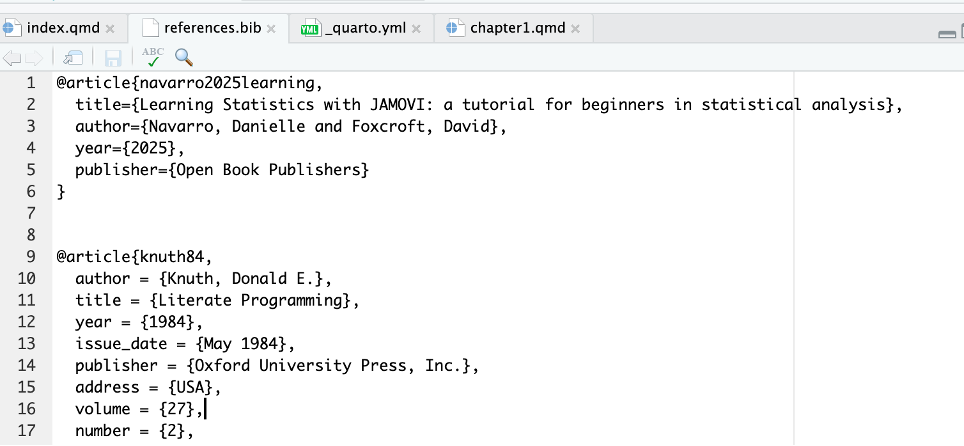
\includegraphics[keepaspectratio]{images/clipboard-3663053904.png}}

references.bib

\begin{itemize}
\tightlist
\item
  tiedostoon voidaan lisätä lähteitä bib text muodossa
\end{itemize}

\pandocbounded{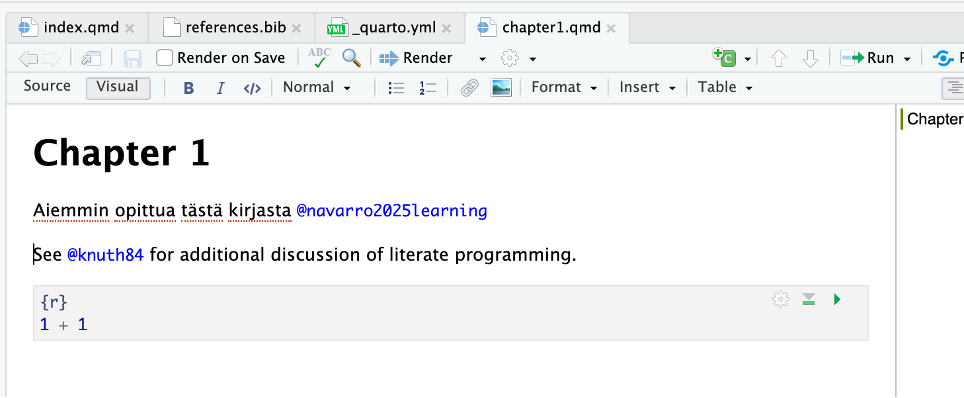
\includegraphics[keepaspectratio]{images/clipboard-1143546947.png}}

\begin{itemize}
\tightlist
\item
  lähteisiin voidaan viitata @ merkillä ja nimellä, jolloin ne näkyvät
  näin:
\end{itemize}

\pandocbounded{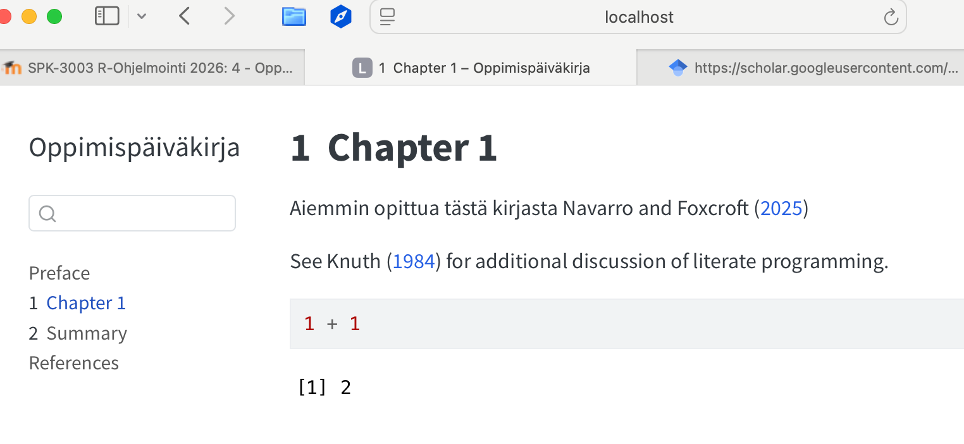
\includegraphics[keepaspectratio]{images/clipboard-12089599.png}}

\pandocbounded{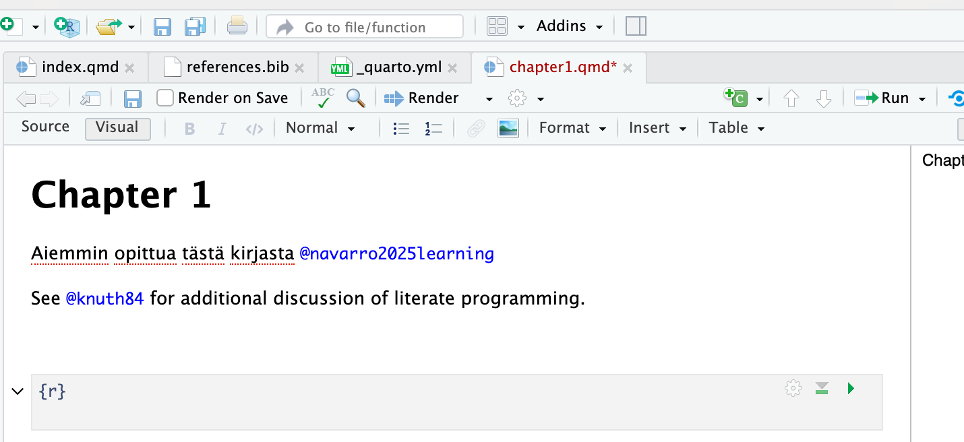
\includegraphics[keepaspectratio]{images/clipboard-486244988.png}}

\begin{itemize}
\item
  yläoikealla olevasta vihreästä c kuvakkeesta voidaan lisätä
  koodinpätkiä

  \begin{itemize}
  \tightlist
  \item
    se lisää alhaalla näkyvän harmaan laatikon, johon voi kirjoittaa
    r-koodia (voi valita muitakin ohjelmointikieliä)
  \end{itemize}
\end{itemize}

\begin{Shaded}
\begin{Highlighting}[]
\DecValTok{1} \SpecialCharTok{+} \DecValTok{1} 
\end{Highlighting}
\end{Shaded}

\begin{verbatim}
[1] 2
\end{verbatim}

\begin{Shaded}
\begin{Highlighting}[]
\DecValTok{2} \SpecialCharTok{*} \DecValTok{2}
\end{Highlighting}
\end{Shaded}

\begin{verbatim}
[1] 4
\end{verbatim}

\begin{Shaded}
\begin{Highlighting}[]
\DecValTok{4} \SpecialCharTok{/} \DecValTok{5} 
\end{Highlighting}
\end{Shaded}

\begin{verbatim}
[1] 0.8
\end{verbatim}

\begin{itemize}
\item
  Lisätyt koodinpätkät näyttävät tältä.
\item
  Jos haluaa koodinpätkän, jota ei suoriteta kannattaa käyttää komentoa

  \begin{itemize}
  \tightlist
  \item
    \#\textbar{} eval: false
  \end{itemize}
\end{itemize}

\begin{Shaded}
\begin{Highlighting}[]
\FunctionTok{install.packages}\NormalTok{(}\FunctionTok{c}\NormalTok{(}\StringTok{"swirl"}\NormalTok{, }\StringTok{"swirlify"}\NormalTok{))}
\FunctionTok{library}\NormalTok{(swirl)}
\FunctionTok{library}\NormalTok{(swirlify)}
\NormalTok{swirl}\SpecialCharTok{::}\FunctionTok{install\_course}\NormalTok{(}\StringTok{"R Programming"}\NormalTok{)}
\NormalTok{swirl}\SpecialCharTok{::}\FunctionTok{install\_course}\NormalTok{(}\StringTok{"The R Programming Environment"}\NormalTok{)}
\NormalTok{swirl}\SpecialCharTok{::}\FunctionTok{install\_course}\NormalTok{(}\StringTok{"Advanced R Programming"}\NormalTok{)}
\FunctionTok{swirl}\NormalTok{()}
\end{Highlighting}
\end{Shaded}

\begin{itemize}
\item
  Nyt boksiin laitettua koodinpätkää ei suoriteta, mutta näyttää
  kuitenkin hyvältä ja sen voi suoraan kopioida
\item
  Yllä näkyvä swirl paketti on R-kielen opetuspaketti. Sen avulla voi
  myös opetella kieltä.
\end{itemize}

\pandocbounded{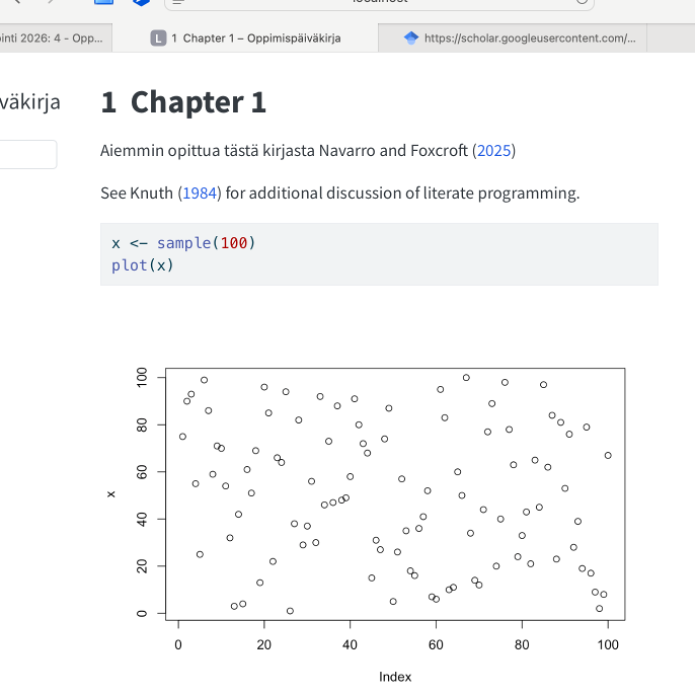
\includegraphics[keepaspectratio]{images/clipboard-4286453426.png}}

\begin{itemize}
\item
  koodi näkyy kirjassa yllä olevalla tavalla

  \begin{itemize}
  \tightlist
  \item
    harmaan koodipalkin oikeasta reunasta voi kopsata koodin
  \end{itemize}
\end{itemize}

\chapter{Osa 2 - R-ohjelmoinnin
perusteet}\label{osa-2---r-ohjelmoinnin-perusteet}

R-ohjelmointikielen kurssin toisen viikon muistiinpanot ja tehtävät.

\section{Apply, quantile \& aggregate}\label{apply-quantile-aggregate}

Ensiksi luotiin datafreimi data.frame() funktiolla

\begin{Shaded}
\begin{Highlighting}[]
\NormalTok{data }\OtherTok{\textless{}{-}} \FunctionTok{data.frame}\NormalTok{(}
  \AttributeTok{Group =} \FunctionTok{as.factor}\NormalTok{(}\FunctionTok{rep}\NormalTok{(}\FunctionTok{c}\NormalTok{(}\StringTok{"GroupA"}\NormalTok{,}\StringTok{"GroupB"}\NormalTok{,}\StringTok{"GroupC"}\NormalTok{),}\DecValTok{10}\NormalTok{, }\AttributeTok{each=}\DecValTok{10}\NormalTok{)), }
  \AttributeTok{Age =} \FunctionTok{as.numeric}\NormalTok{(}\FunctionTok{sample}\NormalTok{(}\DecValTok{18}\SpecialCharTok{:}\DecValTok{65}\NormalTok{, }\DecValTok{300}\NormalTok{, }\AttributeTok{replace=}\ConstantTok{TRUE}\NormalTok{)),}
  \AttributeTok{WM =}  \FunctionTok{as.numeric}\NormalTok{(}\FunctionTok{sample}\NormalTok{(}\DecValTok{1}\SpecialCharTok{:}\DecValTok{100}\NormalTok{, }\DecValTok{300}\NormalTok{, }\AttributeTok{replace=}\ConstantTok{TRUE}\NormalTok{))}
\NormalTok{)}

\FunctionTok{aggregate}\NormalTok{(Age }\SpecialCharTok{\textasciitilde{}}\NormalTok{ Group, }\AttributeTok{data =}\NormalTok{ data, }\AttributeTok{FUN =}\NormalTok{ mean)}
\end{Highlighting}
\end{Shaded}

\begin{verbatim}
   Group   Age
1 GroupA 42.80
2 GroupB 42.72
3 GroupC 43.70
\end{verbatim}

\begin{Shaded}
\begin{Highlighting}[]
\FunctionTok{quantile}\NormalTok{(data}\SpecialCharTok{$}\NormalTok{WM, }\AttributeTok{probs =} \FunctionTok{seq}\NormalTok{(}\DecValTok{0}\NormalTok{, }\DecValTok{1}\NormalTok{, }\FloatTok{0.9}\NormalTok{))}
\end{Highlighting}
\end{Shaded}

\begin{verbatim}
 0% 90% 
  1  92 
\end{verbatim}

\begin{Shaded}
\begin{Highlighting}[]
\FunctionTok{apply}\NormalTok{(data[,}\DecValTok{2}\SpecialCharTok{:}\DecValTok{3}\NormalTok{], }\DecValTok{2}\NormalTok{, mean) }
\end{Highlighting}
\end{Shaded}

\begin{verbatim}
     Age       WM 
43.07333 50.77333 
\end{verbatim}

Aggregate funktiossa ensiksi valitaan numeerinen freimi datasetistä,
josta keskiarvo (tai jokin muu) lasketaan, sitten \textasciitilde{}
merkin jälkeen \# ryhmittelevä tekijä, eli se minkä mukaan data
jaotellaan. \# data = kohtaan datasetti, \# FUN = kohtaan käytettävä
funktio, jota käytetään.

Quantile fuktiolla saadaan laskettua kvantiili. Quantile funktiossa
ensiksi valitaan data, josta kvantiili otetaan. Kohtaan seq( ,
,kolmanteen väliin kvantiili, joka halutaan)

Apply funktiolla voidaan käyttää haluttua funktiota datasetin
valittuihin riveihin tai sarakkeisiin. Apply funktiossa ensiksi
datasetti, {[}hakasulkeissa{]} voidaan indeksien avulla määritellä \#
mitkä rivit tai sarakkeet datasta otetaan käyttöön. Menee aina näin:
{[}rivit, sarakkeet{]} Nyt valittiin {[}2:3{]} komennolla 2. ja 3.
sarake datasta Ekan pilkun jälkeen laitetaan 1 tai 2. Jos laitetaan 1,
niin silloin jaotellaan data rivien mukaan. Jos taas 2, niin se
jaotellaan sarakkeiden mukaan.

\subsection{Teoriaa kvantiileista}\label{teoriaa-kvantiileista}

Kvantiilit / persentiilit

\begin{itemize}
\item
  x-Kvantiili kuvaa sitä pistettä jonka alle jää x prosenttiosuus ja
  ylle y prosenttiosuus havainnoista (y= 100\%-x)

  \begin{itemize}
  \item
    esim. mediaanin (50-persentiili) alle jää 50 \% havainnoista ja ylle
    50\%
  \item
    tai 90-persentiilin alle 90\% ja ylle 10\%
  \item
    Esim.

    \begin{itemize}
    \item
      Manuaalisesti saadaan haettua siten, että asetetaan luvut
      suuruusjärjestykseen ja etsitään oikea kohta. Esim 7 luvun
      sarjassa (1,2,3,4,5,6,7) mediaani on 4. Yläpuolelle jää 3 lukua ja
      alapuolelle 3.
    \item
      90.-persentiili sarjassa (1,2,3,4,5,6,7) asettuu lukujen 6 ja 7
      välille. Kun luku ei osu suoraan kohdalle täytyy se interpoloida.
    \end{itemize}
  \item
    kvantiili kuvaa siis alueiden rajalla olevaa pistettä
  \end{itemize}
\item
  R-kielellä kvantiilin saa etsittyä quantile() funktiolla
\end{itemize}

\begin{Shaded}
\begin{Highlighting}[]
\FunctionTok{quantile}\NormalTok{(}\FunctionTok{c}\NormalTok{(}\DecValTok{1}\NormalTok{,}\DecValTok{2}\NormalTok{,}\DecValTok{3}\NormalTok{,}\DecValTok{4}\NormalTok{,}\DecValTok{5}\NormalTok{,}\DecValTok{6}\NormalTok{,}\DecValTok{7}\NormalTok{), }\AttributeTok{probs =} \FunctionTok{seq}\NormalTok{(}\DecValTok{0}\NormalTok{, }\DecValTok{1}\NormalTok{, }\FloatTok{0.5}\NormalTok{), }\AttributeTok{na.rm =} \ConstantTok{FALSE}\NormalTok{,}
         \AttributeTok{names =} \ConstantTok{TRUE}\NormalTok{)}
\end{Highlighting}
\end{Shaded}

\begin{verbatim}
  0%  50% 100% 
   1    4    7 
\end{verbatim}

\begin{Shaded}
\begin{Highlighting}[]
    \FunctionTok{quantile}\NormalTok{(x, }\AttributeTok{prob =} \FunctionTok{seq}\NormalTok{(}\DecValTok{0}\NormalTok{, }\DecValTok{1}\NormalTok{, }\FloatTok{0.5}\NormalTok{), }\AttributeTok{na.rm =} \ConstantTok{FALSE}\NormalTok{, }
  \AttributeTok{names =} \ConstantTok{TRUE}\NormalTok{, }\AttributeTok{type =} \DecValTok{7}\NormalTok{)}
\end{Highlighting}
\end{Shaded}

\begin{itemize}
\item
  x = data/vektori, josta kvantiili otetaan
\item
  probs = seq(0, 1, 0.25) --\textgreater{} ekat kaksi numeroa pidetään
  aina 0 ja ykkösenä. Määrittää sekvenssin rajat. Viimeinen luku
  määrittää miten sekvenssi jaetaan

  \begin{itemize}
  \item
    toisin sanottonu 0,25 kohtaan laitetaan haluttu kvantiili

    \begin{itemize}
    \item
      0,25 niin tulee persentiilit 25\% välein
    \item
      0,90 tulee 90-persentiili ja 0,5 mediaani
    \end{itemize}
  \end{itemize}
\item
  na.rm = FALSE, saa tarvittaessa puuttuvat arvot jätettyä huomiotta.
  Tällöin merkattava TRUE, jolloin poistaa puuttuvat arvot.
\item
  names = TRUE, näyttää prosentit
\item
  type =, valitaan tyyppi, toimii ilmankin.
\end{itemize}

seq()

\begin{Shaded}
\begin{Highlighting}[]
\FunctionTok{seq}\NormalTok{(}\DecValTok{0}\NormalTok{,}\DecValTok{10}\NormalTok{,}\DecValTok{3}\NormalTok{)}
\end{Highlighting}
\end{Shaded}

\begin{verbatim}
[1] 0 3 6 9
\end{verbatim}

\begin{Shaded}
\begin{Highlighting}[]
\CommentTok{\#sekvenssi, 1. numero kertoo alkupisteen, toinen loppupisteen ja 3. numero}
\CommentTok{\#   sen millä välein sekvenssi jatkuu eli numerot lisätään. }
\end{Highlighting}
\end{Shaded}

\begin{Shaded}
\begin{Highlighting}[]
\FunctionTok{rep}\NormalTok{(}\DecValTok{1}\SpecialCharTok{:}\DecValTok{4}\NormalTok{,}\AttributeTok{times =}\DecValTok{3}\NormalTok{)}
\end{Highlighting}
\end{Shaded}

\begin{verbatim}
 [1] 1 2 3 4 1 2 3 4 1 2 3 4
\end{verbatim}

\begin{Shaded}
\begin{Highlighting}[]
\CommentTok{\#Repeat a vector ; 1. mitä toistetaan, 2. montako kertaa voi kirjoittaa times =, tai pelkästään numeron toimii molemmilla }


\FunctionTok{rep}\NormalTok{(}\DecValTok{1}\SpecialCharTok{:}\DecValTok{3}\NormalTok{, }\AttributeTok{each=}\DecValTok{5}\NormalTok{)}
\end{Highlighting}
\end{Shaded}

\begin{verbatim}
 [1] 1 1 1 1 1 2 2 2 2 2 3 3 3 3 3
\end{verbatim}

\begin{Shaded}
\begin{Highlighting}[]
\CommentTok{\#Repeat elements of a vector: 1. mitä toistetaan 2. each =, komennolla toistetaan jokainen elementti haluttu määrä kertoja }
\end{Highlighting}
\end{Shaded}

list()

\begin{Shaded}
\begin{Highlighting}[]
\NormalTok{l }\OtherTok{\textless{}{-}} \FunctionTok{list}\NormalTok{(}\AttributeTok{x =} \DecValTok{1}\SpecialCharTok{:}\DecValTok{5}\NormalTok{, }\AttributeTok{y =} \FunctionTok{c}\NormalTok{(}\StringTok{\textquotesingle{}a\textquotesingle{}}\NormalTok{, }\StringTok{\textquotesingle{}b\textquotesingle{}}\NormalTok{), }\AttributeTok{z =} \FunctionTok{rep}\NormalTok{(}\DecValTok{1}\SpecialCharTok{:}\DecValTok{4}\NormalTok{,}\AttributeTok{times =}\DecValTok{3}\NormalTok{))}
\NormalTok{l}
\end{Highlighting}
\end{Shaded}

\begin{verbatim}
$x
[1] 1 2 3 4 5

$y
[1] "a" "b"

$z
 [1] 1 2 3 4 1 2 3 4 1 2 3 4
\end{verbatim}

list() funktio tekee annetuista syötteistä listat. Voivat olla erilaisia
ja eri mittaisia.

\begin{Shaded}
\begin{Highlighting}[]
\NormalTok{my\_list }\OtherTok{\textless{}{-}} \FunctionTok{list}\NormalTok{(}\AttributeTok{a =} \DecValTok{1}\NormalTok{, }\AttributeTok{b =} \DecValTok{2}\NormalTok{, }\AttributeTok{c =} \DecValTok{3}\NormalTok{)}
\NormalTok{my\_list}\SpecialCharTok{$}\NormalTok{d }\OtherTok{\textless{}{-}} \DecValTok{4}
\NormalTok{my\_list}
\end{Highlighting}
\end{Shaded}

\begin{verbatim}
$a
[1] 1

$b
[1] 2

$c
[1] 3

$d
[1] 4
\end{verbatim}

Lisätään listaan uusi alkio Salmela (2026) tyyli

\begin{Shaded}
\begin{Highlighting}[]
\NormalTok{lista }\OtherTok{\textless{}{-}} \FunctionTok{list}\NormalTok{(}\AttributeTok{x =} \DecValTok{1}\SpecialCharTok{:}\DecValTok{5}\NormalTok{, }\AttributeTok{y =} \DecValTok{6}\SpecialCharTok{:}\DecValTok{10}\NormalTok{)}
\NormalTok{lista }\OtherTok{\textless{}{-}} \FunctionTok{c}\NormalTok{(lista, }\FunctionTok{list}\NormalTok{(}\AttributeTok{z =} \DecValTok{50}\SpecialCharTok{:}\DecValTok{55}\NormalTok{))}
\NormalTok{lista}
\end{Highlighting}
\end{Shaded}

\begin{verbatim}
$x
[1] 1 2 3 4 5

$y
[1]  6  7  8  9 10

$z
[1] 50 51 52 53 54 55
\end{verbatim}

Toinen mahdollinen tyyli lisätä alkio listaan.

\subsection{Pylväsdiagrammin
piirtäminen}\label{pylvuxe4sdiagrammin-piirtuxe4minen}

\begin{Shaded}
\begin{Highlighting}[]
\NormalTok{heights\_var }\OtherTok{\textless{}{-}} \FunctionTok{c}\NormalTok{(}\DecValTok{150}\NormalTok{, }\DecValTok{160}\NormalTok{, }\DecValTok{170}\NormalTok{, }\DecValTok{180}\NormalTok{, }\DecValTok{190}\NormalTok{)}
\FunctionTok{barplot}\NormalTok{(heights\_var)}
\end{Highlighting}
\end{Shaded}

\pandocbounded{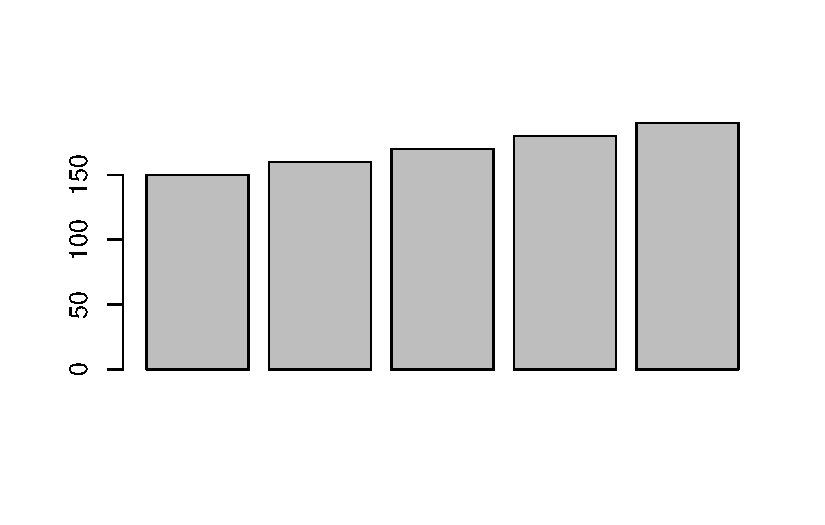
\includegraphics[keepaspectratio]{R_kurssi/Osa02_files/figure-pdf/unnamed-chunk-9-1.pdf}}

\subsection{Dataframen tallentaminen .csv
muotoon}\label{dataframen-tallentaminen-.csv-muotoon}

\begin{Shaded}
\begin{Highlighting}[]
\NormalTok{df }\OtherTok{\textless{}{-}} \FunctionTok{data.frame}\NormalTok{(}\AttributeTok{name =} \FunctionTok{c}\NormalTok{(}\StringTok{"John"}\NormalTok{, }\StringTok{"Jane"}\NormalTok{, }\StringTok{"Doe"}\NormalTok{), }\AttributeTok{age =} \FunctionTok{c}\NormalTok{(}\DecValTok{23}\NormalTok{, }\DecValTok{25}\NormalTok{, }\DecValTok{28}\NormalTok{))}
\FunctionTok{write.csv}\NormalTok{(df, }\StringTok{"new\_data.csv"}\NormalTok{)}
\end{Highlighting}
\end{Shaded}

\begin{itemize}
\item
  write.csv() komennolla: ekaan väliin tallennettava data, tokaan väliin
  luotavan tiedoston nimi
\item
  write.csv() luomassa tiedostossa piste (.) toimii desimaalien
  erottajana ja pilkku (,) sarakkeiden erottelijana.
\item
  write.csv2() käyttää suomalaistyyliin pilkkua (,)
  desimaalierottelijana ja puolipistettä (;) sarakkeiden erottelijana

  \begin{itemize}
  \item
    voi olla hyödyllinen, kun halutaan viedä suomenkieliseen exceliin.
  \item
    tosin excel kysyy csv. tiedostoa tuotaessa, että millä se erotellaan
  \end{itemize}
\end{itemize}

\section{Luento 2}\label{luento-2}

kysy havaintojen lukumäärä

\begin{Shaded}
\begin{Highlighting}[]
\NormalTok{nObs }\OtherTok{\textless{}{-}} \FunctionTok{readline}\NormalTok{(}\AttributeTok{prompt =} \StringTok{"Anna havaintojen lukumäärä: "}\NormalTok{)}
\end{Highlighting}
\end{Shaded}

muodosta tyhjä vektori havaintojen arvojen tallentamista varten

\begin{Shaded}
\begin{Highlighting}[]
\NormalTok{MyVar }\OtherTok{\textless{}{-}} \FunctionTok{numeric}\NormalTok{(nObs)}
\end{Highlighting}
\end{Shaded}

tee loop, jossa kysytään jokaisen havainnon arvo

\begin{Shaded}
\begin{Highlighting}[]
\ControlFlowTok{for}\NormalTok{ (i }\ControlFlowTok{in} \DecValTok{1}\SpecialCharTok{:}\NormalTok{nObs) \{ MyVar[i] }\OtherTok{\textless{}{-}} \FunctionTok{readline}\NormalTok{(}\AttributeTok{prompt =} \FunctionTok{paste}\NormalTok{(}\StringTok{\textquotesingle{}Anna havainnon\textquotesingle{}}\NormalTok{, i, }\StringTok{\textquotesingle{}arvo: \textquotesingle{}}\NormalTok{)) \}}
\end{Highlighting}
\end{Shaded}

talleta arvot datakehikkoon

\begin{Shaded}
\begin{Highlighting}[]
\NormalTok{data3 }\OtherTok{\textless{}{-}} \FunctionTok{data.frame}\NormalTok{(}\AttributeTok{Kurssipisteet =}\NormalTok{ MyVar)}
\end{Highlighting}
\end{Shaded}

tulosta konsoliin

\begin{Shaded}
\begin{Highlighting}[]
\FunctionTok{print}\NormalTok{(data3)}
\end{Highlighting}
\end{Shaded}

\subsection{\texorpdfstring{\textbf{2. osan
datansyöttötehtävä}}{2. osan datansyöttötehtävä}}\label{osan-datansyuxf6ttuxf6tehtuxe4vuxe4}

Tehtävänanto:

Tee ohjelma, jolla voit syöttää muuttujalle arvot. Eli ohjelma ensin
kysyy käyttäjältä kuinka monta havaintoa talletetaan ja sitten ohjelma
kysyy jokaisen havainnon arvon. Ja nämä talletetaan data.frame:en.
lopuksi skripti tulostaa datan. palauta R-skripti

Lisähaasteena voit tehdä niin, että ohjelma kysyy kuinka monta muuttujaa
talletetaan, ja muuttujien nimet, ja sitten vuorotellen kaikille
muuttujille havaintojen arvot.~

Tarpeellisia funktiota voi olla: readline() , esim: readline(prompt =
``Anna havaintojen määrä:'') data.frame() , uuden data-kehikon luominen
paste() , muuttujien yhdistäminen, esim. paste(``Anna havainnon'', i,
``arvo:'') for-loop, esim.~

for (i in 1:num\_obs) \{\\
\strut ~ \ldots.\\
\} names(data) , data-kehikon muuttujien nimet print()

Ratkaisu:

\begin{Shaded}
\begin{Highlighting}[]
\CommentTok{\#kysy havaintojen lukumäärä }
\NormalTok{nObs }\OtherTok{\textless{}{-}}\FunctionTok{as.numeric}\NormalTok{(}\FunctionTok{readline}\NormalTok{(}\AttributeTok{prompt =} \StringTok{"Anna havaintojen lukumäärä: "}\NormalTok{))}

\CommentTok{\#kysy muuttujien lukumäärä }

\NormalTok{MuutLkm }\OtherTok{\textless{}{-}} \FunctionTok{as.numeric}\NormalTok{(}\FunctionTok{readline}\NormalTok{(}\AttributeTok{prompt =} \StringTok{"Anna muuttujien lukumäärä: "}\NormalTok{))}

\CommentTok{\#muuttujien nimet }

\NormalTok{MuutNimet }\OtherTok{\textless{}{-}} \FunctionTok{character}\NormalTok{(MuutLkm)}

\ControlFlowTok{for}\NormalTok{ (i }\ControlFlowTok{in} \DecValTok{1}\SpecialCharTok{:}\NormalTok{MuutLkm)\{}
  
\NormalTok{  MuutNimet[i] }\OtherTok{\textless{}{-}} \FunctionTok{readline}\NormalTok{( }\AttributeTok{prompt =} \FunctionTok{paste}\NormalTok{(}\StringTok{\textquotesingle{}Anna muuttujan\textquotesingle{}}\NormalTok{,i, }\StringTok{\textquotesingle{}nimi: \textquotesingle{}}\NormalTok{))}
\NormalTok{  \}}

\CommentTok{\#luodaan datafreimi}

\NormalTok{datafreimi }\OtherTok{\textless{}{-}} \FunctionTok{data.frame}\NormalTok{(}\FunctionTok{matrix}\NormalTok{(}\AttributeTok{nrow =}\NormalTok{ nObs, }\AttributeTok{ncol =}\NormalTok{ MuutLkm,))}
\FunctionTok{colnames}\NormalTok{(datafreimi) }\OtherTok{\textless{}{-}}\NormalTok{ MuutNimet}

\CommentTok{\#lisätään havaintoarvot datafremiin muuttuja kerrallaan}

\ControlFlowTok{for}\NormalTok{ (i }\ControlFlowTok{in} \DecValTok{1}\SpecialCharTok{:}\NormalTok{MuutLkm)\{ }
  \ControlFlowTok{for}\NormalTok{ (j }\ControlFlowTok{in} \DecValTok{1}\SpecialCharTok{:}\NormalTok{nObs)\{}
\NormalTok{    datafreimi[j,i] }\OtherTok{\textless{}{-}} \FunctionTok{readline}\NormalTok{(}\AttributeTok{prompt =} \FunctionTok{paste}\NormalTok{(}\StringTok{"anna muuttujan"}\NormalTok{, MuutNimet[i], }\StringTok{"havainnon"}\NormalTok{, j, }\StringTok{"arvo: "}\NormalTok{))  }
    
\NormalTok{  \}}
  
\NormalTok{\}}

\FunctionTok{print}\NormalTok{(datafreimi)}
\end{Highlighting}
\end{Shaded}

\section{Funktiot: readline(), paste(), data.frame(), for loop()\{\},
as.numeric(), numeric(), character(),
matrix()}\label{funktiot-readline-paste-data.frame-for-loop-as.numeric-numeric-character-matrix}

\begin{Shaded}
\begin{Highlighting}[]
\NormalTok{nObs }\OtherTok{\textless{}{-}} \FunctionTok{as.numeric}\NormalTok{(}\FunctionTok{readline}\NormalTok{(}\AttributeTok{prompt =} \StringTok{"Anna havaintojen lukumäärä: "}\NormalTok{))}
\end{Highlighting}
\end{Shaded}

readline()

\begin{itemize}
\item
  R-kielen komento, jonka avulla ohjelma pysähtyy ja odottaa, että
  käyttäjä kirjoittaa jotain näppäimistöllä konsoliin.
\item
  Kun R kohtaa~readline()-komennon, se ei jatka koodin suorittamista
  ennen kuin painat~Enter. Kaikki, mitä kirjoitat ennen Enteriä,
  tallennetaan muuttujaan.
\item
  Tärkeää muistaa: Se palauttaa aina tekstiä

  \begin{itemize}
  \item
    Tämä on yleisin virhe readline()-funktion kanssa. Vaikka
    kirjoittaisit numeron (esim. 25), R tallentaa sen tekstinä (``25''),
    ei lukuna.
  \item
    Jos haluat käyttää syötettä laskutoimituksissa, sinun täytyy muuttaa
    se numeroksi~as.numeric()-funktiolla:
  \end{itemize}
\end{itemize}

prompt =

\begin{itemize}
\item
  On tärkeää huomata, että R-kielessä prompt ei ole itsenäinen
  ``komento'' samalla tavalla kuin vaikkapa print(), vaan se on
  \textbf{argumentti} (eli lisäasetus), jota käytetään muiden
  funktioiden sisällä.
\item
  Yleisimmin esiintyy readline()-funktion yhteydessä.
\item
  Prompt tarkoittaa suomeksi \textbf{kehotetta}. Sen tehtävä on kertoa
  käyttäjälle, mitä hänen odotetaan tekevän. Se tulostaa tekstin
  konsoliin ja jättää kursorin odottamaan käyttäjän kirjoitusta.

  Ilman prompt-asetusta tietokone vain pysähtyisi odottamaan syötettä,
  ja käyttäjä olisi ihmeissään, miksi mitään ei tapahdu.
\end{itemize}

as.numeric()

\begin{itemize}
\item
  muuttaa syötteen tekstista numeeriseksi
\item
  tämän myötä esimerkiksi laskutoimitukset onnistuvat
\end{itemize}

\begin{Shaded}
\begin{Highlighting}[]
\FunctionTok{numeric}\NormalTok{(}\DecValTok{5}\NormalTok{)}
\end{Highlighting}
\end{Shaded}

\begin{verbatim}
[1] 0 0 0 0 0
\end{verbatim}

numeric()

\begin{itemize}
\item
  Luo tyhjän numeerisen vektorin, jonka voi täyttää
\item
  Sulkuihin voi määritellä montako paikkaa vektoriin tulee

  \begin{itemize}
  \tightlist
  \item
    esim. numeric(5) luo vektorin, jossa 5 nollaa eli 5 tyhjää paikkaa
    täytettäväksi
  \item
    voi laittaa myös muuttujan sulkeisiin, jolloin paikkoja tulee
    muuttujan arvon verran
  \end{itemize}
\end{itemize}

\begin{Shaded}
\begin{Highlighting}[]
\FunctionTok{character}\NormalTok{(}\DecValTok{6}\NormalTok{)}
\end{Highlighting}
\end{Shaded}

\begin{verbatim}
[1] "" "" "" "" "" ""
\end{verbatim}

character()

\begin{itemize}
\item
  Luo tyhjän tekstipohjaisen ``vektorin'' / listan, jossa ennalta
  määritelty määrä paikkoja
\item
  esim character(6) vektorissa 6 paikkaa
\item
  Sulkuihin voi laittaa myös muuttujan, jolloin paikkojen lukumäärä
  tulee muuttujan arvon mukaan esim. character(Muuttuja)
\end{itemize}

\begin{Shaded}
\begin{Highlighting}[]
\NormalTok{datafreimi }\OtherTok{\textless{}{-}} \FunctionTok{data.frame}\NormalTok{(}\FunctionTok{matrix}\NormalTok{(}\AttributeTok{nrow =}\NormalTok{ nObs, }\AttributeTok{ncol =}\NormalTok{ MuutLkm,))}
\FunctionTok{colnames}\NormalTok{(datafreimi) }\OtherTok{\textless{}{-}}\NormalTok{ MuutNimet}
\end{Highlighting}
\end{Shaded}

data.frame()

\begin{itemize}
\item
  luo dataframen
\item
  \textbf{Sarakkeiden määrä}~määräytyy siitä, kuinka monta vektoria
  annat syötteeksi.
\end{itemize}

\begin{itemize}
\tightlist
\item
  \textbf{Rivien määrä}~määräytyy annettujen vektorien pituudesta.
\end{itemize}

\begin{Shaded}
\begin{Highlighting}[]
 \FunctionTok{data.frame}\NormalTok{(}\AttributeTok{Eka =} \FunctionTok{c}\NormalTok{(}\DecValTok{3}\NormalTok{,}\DecValTok{4}\NormalTok{,}\DecValTok{5}\NormalTok{,}\DecValTok{2}\NormalTok{),}
            \AttributeTok{Toka =} \FunctionTok{seq}\NormalTok{(}\DecValTok{2}\NormalTok{,}\DecValTok{8}\NormalTok{,}\DecValTok{2}\NormalTok{), }
            \AttributeTok{Kolmas =} \FunctionTok{c}\NormalTok{(}\StringTok{"Matti"}\NormalTok{, }\StringTok{"Jesse"}\NormalTok{, }\StringTok{"Katja"}\NormalTok{, }\StringTok{"Joni"}\NormalTok{)}
\NormalTok{            )}
\end{Highlighting}
\end{Shaded}

\begin{verbatim}
  Eka Toka Kolmas
1   3    2  Matti
2   4    4  Jesse
3   5    6  Katja
4   2    8   Joni
\end{verbatim}

\begin{itemize}
\item
  Yllä olevaan frameen laitettiin kolme vektoria, jotka kaikki olivat
  pituudeltaan 4 alkiota, joten syntyi kolmen sarakkeen ja neljän rivin
  datafreimi.
\item
  Sarakkeet pystyy nimeämään luomisvaiheessa (Eka, Toka, Kolmas) tai
  myöhemmin colnames() funktiolla
\end{itemize}

\begin{Shaded}
\begin{Highlighting}[]
\NormalTok{df }\OtherTok{\textless{}{-}} \FunctionTok{data.frame}\NormalTok{(}\FunctionTok{matrix}\NormalTok{(}\AttributeTok{nrow =} \DecValTok{5}\NormalTok{, }\AttributeTok{ncol =} \DecValTok{5}\NormalTok{))}
\FunctionTok{colnames}\NormalTok{(df) }\OtherTok{\textless{}{-}} \FunctionTok{c}\NormalTok{(}\StringTok{"Ikä"}\NormalTok{, }\StringTok{"Pituus"}\NormalTok{, }\StringTok{"Paino"}\NormalTok{, }\StringTok{"Ekstroversio"}\NormalTok{, }\StringTok{"Avoimuus"}\NormalTok{)}
\NormalTok{df}
\end{Highlighting}
\end{Shaded}

\begin{verbatim}
  Ikä Pituus Paino Ekstroversio Avoimuus
1  NA     NA    NA           NA       NA
2  NA     NA    NA           NA       NA
3  NA     NA    NA           NA       NA
4  NA     NA    NA           NA       NA
5  NA     NA    NA           NA       NA
\end{verbatim}

\begin{itemize}
\tightlist
\item
  Halutessaan dataframeen voi valmiiksi määrittää pohjalle tietyn määrän
  rivejä ja sarakkeita matrix() funktion avulla
\end{itemize}

\begin{itemize}
\item
  matrix(nrow = 5, ncol = 5)

  \begin{itemize}
  \tightlist
  \item
    nrow ja ncol määrittävät rivien ja sarakkeiden lukumäärän
  \end{itemize}
\item
  colnames() funktiolla saa sarakkeiden nimet määritettyä
\item
  c() komento yhdistää sisällön yhdeksi vektoriksi
\end{itemize}

paste()

\begin{Shaded}
\begin{Highlighting}[]
\FunctionTok{print}\NormalTok{(}\FunctionTok{paste}\NormalTok{(}\StringTok{"Hei,"}\NormalTok{, nimi)}
\end{Highlighting}
\end{Shaded}

\chapter{Osa 3 - Raja-arvolause ja
permutaatiotesti}\label{osa-3---raja-arvolause-ja-permutaatiotesti}

Osan 3 muistiinpanot ja tehtävät.

\section{Osa 3. alkutehtävät}\label{osa-3.-alkutehtuxe4vuxe4t}

Tehtävänanto: Kirjoita R-skripti, joka kysyy numeroa ja kertoo onko
numero positiinen vai negatiivinen.

\begin{Shaded}
\begin{Highlighting}[]
\NormalTok{Num }\OtherTok{\textless{}{-}} \FunctionTok{as.numeric}\NormalTok{(}\FunctionTok{readline}\NormalTok{(}\AttributeTok{prompt =} \StringTok{"Syötä numero: "}\NormalTok{))}

\ControlFlowTok{if}\NormalTok{ (Num }\SpecialCharTok{==} \DecValTok{0}\NormalTok{)\{ }\FunctionTok{print}\NormalTok{(}\StringTok{"Nolla"}\NormalTok{) \} }\ControlFlowTok{else}\NormalTok{ \{}

\ControlFlowTok{if}\NormalTok{ (Num }\SpecialCharTok{\textgreater{}} \DecValTok{0}\NormalTok{)\{}
  \FunctionTok{print}\NormalTok{(}\StringTok{"positiivinen"}\NormalTok{)}
\NormalTok{\} }\ControlFlowTok{else}\NormalTok{ \{}
  \FunctionTok{print}\NormalTok{(}\StringTok{"negatiivinen"}\NormalTok{)}
\NormalTok{\} }

\NormalTok{\}}
\end{Highlighting}
\end{Shaded}

Tehtävänanto: Kirjoita R-skripti, joka kysyy kurssin arvosanaa (0-100)
\#ja kertoo onko kurssin suoritus hyväksytty vain hylätty. \#Opiskelijan
pitää saada vähintään 50 pistettä.

\begin{Shaded}
\begin{Highlighting}[]
\NormalTok{Num }\OtherTok{\textless{}{-}} \FunctionTok{as.numeric}\NormalTok{(}\FunctionTok{readline}\NormalTok{(}\AttributeTok{prompt =} \StringTok{"Syötä kurssin arvosana 0{-}100: "}\NormalTok{))}

\ControlFlowTok{if}\NormalTok{ (Num }\SpecialCharTok{\textless{}} \DecValTok{50}\NormalTok{)\{ }\FunctionTok{print}\NormalTok{(}\StringTok{"Hylätty"}\NormalTok{) \}}\ControlFlowTok{else}\NormalTok{ \{ }\FunctionTok{print}\NormalTok{(}\StringTok{"Hyväksytty"}\NormalTok{) \}}
\end{Highlighting}
\end{Shaded}

Tehtävänanto: Kirjoita R-skripti, joka kysyy numeroa ja kertoo onko
numero parillinen vai pariton.

\begin{Shaded}
\begin{Highlighting}[]
\NormalTok{Num }\OtherTok{\textless{}{-}} \FunctionTok{as.numeric}\NormalTok{(}\FunctionTok{readline}\NormalTok{(}\AttributeTok{prompt =} \StringTok{"Syötä numero: "}\NormalTok{))}

\ControlFlowTok{if}\NormalTok{ (Num }\SpecialCharTok{\%\%} \DecValTok{2} \SpecialCharTok{==}\DecValTok{0}\NormalTok{)\{ }\FunctionTok{print}\NormalTok{(}\StringTok{"Parillinen"}\NormalTok{) \} }\ControlFlowTok{else}\NormalTok{ \{ }\FunctionTok{print}\NormalTok{(}\StringTok{"Pariton"}\NormalTok{) \}}
\end{Highlighting}
\end{Shaded}

\#parillisuus saadaan tsekattua jakojäännöksellä, jos 2 jaettaessa nolla
-\textgreater{} parillinen \# jakojäännös lasketaan \%\% operaattorilla

10 \%\% 2 10 \%\% 3 11 \%\% 2

\#esim. 10/2 jakojäännös on 0 ; 10/3 jakojäännös 1 ; 11 / 2 jakojäännös
1

Tehtävänanto: Kirjoita for-silmukka, joka tulostaa numerot 1-10.

\begin{Shaded}
\begin{Highlighting}[]
\ControlFlowTok{for}\NormalTok{ (i }\ControlFlowTok{in} \DecValTok{1}\SpecialCharTok{:}\DecValTok{10}\NormalTok{)\{ }\FunctionTok{print}\NormalTok{(i) \}}
\end{Highlighting}
\end{Shaded}

\begin{verbatim}
[1] 1
[1] 2
[1] 3
[1] 4
[1] 5
[1] 6
[1] 7
[1] 8
[1] 9
[1] 10
\end{verbatim}

Tehtävänanto: Kirjoita for-silmukka, joka tulostaa lukujen 1:10 neliön.

\begin{Shaded}
\begin{Highlighting}[]
\ControlFlowTok{for}\NormalTok{ (i }\ControlFlowTok{in} \DecValTok{1}\SpecialCharTok{:}\DecValTok{10}\NormalTok{)\{ }\FunctionTok{print}\NormalTok{(i }\SpecialCharTok{*}\NormalTok{ i ) \}}
\end{Highlighting}
\end{Shaded}

\begin{verbatim}
[1] 1
[1] 4
[1] 9
[1] 16
[1] 25
[1] 36
[1] 49
[1] 64
[1] 81
[1] 100
\end{verbatim}

\begin{Shaded}
\begin{Highlighting}[]
\ControlFlowTok{for}\NormalTok{ (i }\ControlFlowTok{in} \DecValTok{1}\SpecialCharTok{:}\DecValTok{10}\NormalTok{)\{ }\FunctionTok{print}\NormalTok{(i}\SpecialCharTok{\^{}}\DecValTok{2}\NormalTok{ ) \}}
\end{Highlighting}
\end{Shaded}

\begin{verbatim}
[1] 1
[1] 4
[1] 9
[1] 16
[1] 25
[1] 36
[1] 49
[1] 64
[1] 81
[1] 100
\end{verbatim}

\begin{Shaded}
\begin{Highlighting}[]
\ControlFlowTok{for}\NormalTok{ (i }\ControlFlowTok{in} \DecValTok{1}\SpecialCharTok{:}\DecValTok{10}\NormalTok{)\{ }\FunctionTok{print}\NormalTok{(i}\SpecialCharTok{**}\DecValTok{2}\NormalTok{ ) \}}
\end{Highlighting}
\end{Shaded}

\begin{verbatim}
[1] 1
[1] 4
[1] 9
[1] 16
[1] 25
[1] 36
[1] 49
[1] 64
[1] 81
[1] 100
\end{verbatim}

Kolme eri tapaa

Tehtävänanto: Kirjoita for-silmukka, joka laskee lukujen 1:100 summan.

\begin{Shaded}
\begin{Highlighting}[]
\NormalTok{summa }\OtherTok{\textless{}{-}} \DecValTok{0}

\ControlFlowTok{for}\NormalTok{ (i }\ControlFlowTok{in} \DecValTok{1}\SpecialCharTok{:}\DecValTok{100}\NormalTok{)\{ summa }\OtherTok{\textless{}{-}}\NormalTok{ summa }\SpecialCharTok{+}\NormalTok{ i \} }
\FunctionTok{print}\NormalTok{(summa)}
\end{Highlighting}
\end{Shaded}

\begin{verbatim}
[1] 5050
\end{verbatim}

\section{Permutaatiotesti}\label{permutaatiotesti}

\subsection{Teoriaa permutaatiosta}\label{teoriaa-permutaatiosta}

Permutaatio tarkoittaa järjestystä tai uudelleenjärjestelyä

\begin{itemize}
\item
  Esim. lukujoukko (1,2,3) tai kirjainsarja (A, B, C) voivat saada 6 eri
  permutaatiota eli uniikkia järjestystä
\item
  Mahdollisten permutaatioden määrä lasketaan käyttämällä kertomaa
  (merkitään !)
\end{itemize}

P(n)=n!

\begin{itemize}
\tightlist
\item
  missä P tarkoittaa permutaatioden määrää ja n alkioiden lukumäärää
\item
  Esim. kun 4 alkiota lasketaan 4! = 4 * 3 * 2 * 1 = 24
\item
  Tai kun 3 alkiota 3! = 3 * 2 * 1 = 6
\end{itemize}

Kertoma lasketaan R-kielellä factorial() funktiolla

\begin{Shaded}
\begin{Highlighting}[]
\FunctionTok{factorial}\NormalTok{(}\DecValTok{4}\NormalTok{)}
\end{Highlighting}
\end{Shaded}

\begin{verbatim}
[1] 24
\end{verbatim}

Permutaatiotesti on ei-parametrinen eli toimii millä tahansa
aineistoilla

\begin{itemize}
\tightlist
\item
  Datan ei tarvitse siis täyttää normaalisuusoletusta
\end{itemize}

Permutaatiotestillä saadaan laskettua p-arvo eli kuinka todennäköisesti
sattumalta saadaan sama tulos.

Permutaatioiden määrää lisäämällä sadaan p-arvo laskettua tarkemmin.
Viljamin videoilla käytettiin 1000 tai 10 000 permutaatiota.

Thulin (2024) kirjassa neuvotaan nyrkkisääntönä käyttämään 9 999
permutaatiota, koska tällöin p arvo ainakaan usein ei asetu tasan 0,05
vaan sen alle tai yli

\subsection{Permutaatiotesti ja
bootstrap}\label{permutaatiotesti-ja-bootstrap}

Permutaatio tarkoittaa yhtä lukujoukon tai R-kontekstissa vektorin
järjestystä. Kun ne järjestetään uudelleen, saadaan toinen permutaatio.
Esimerkiksi lukujoukolla (1,2,3) on yhteensä kuusi eri permutaatiota.
Tilastotieteessä permutaatiota käytetään etenkin permutaatiotestissä,
jonka avulla voidaan määrittää p-arvo. Permutaatiotesti on siitä, hyvä
työkalu, että se ei oleta aineiston olevan normaalisti jakautunutta, eli
sitä voidaan käyttää käytännössä millä hyvänsä aineistolla.

Esimerkiksi, jos kahdelta ryhmältä on mitattu koesuoritus ja halutaan
tietää, onko ryhmien suoritusten välillä tilastollisesti merkitsevä ero,
niin ensiksi lasketaan suorituspisteiden keskiarvojen erotus. Sen
jälkeen sekoitetaan ryhmätunnisteita siten, että ryhmät jakautuvat esim.
9 999 uuteen permutaatioon ja lasketaan jokaisen permutaation kohdalla
ryhmien keskiarvoero. Sitten verrataan, kuinka moni permutaatioiden
keskiarvoeroista oli yhtä suuria tai suurempia kuin mitattu ero. Mikäli
alle 5 \% permutaatioista oli suurempia tai yhtä suuria kuin mitattu
ero, niin p-arvo on alle 0,05 eli tilastollisesti merkitsevä ja
nollahypoteesi voidaan hylätä.

Bootsrap on hiukan vastaava menetelmä kuin permutaatiotesti, mutta se
eroaa siten, että siinä sekoitusvaiheessa alkiot arvotaan satunnaisesti
uuteen ''otokseen'' siten, että osa saattaa esiintyä useamman kerran ja
osa ei ollenkaan. Eli kun permutaatiotestissä jokaisessa permutaatiossa
on kaikki alkiot mukana, mutta vain eri järjestyksessä, niin
bootstrapissä on hiukan eri kokoelma alkiota valikoituneena
alkuperäisestä otoksesta. Yhdessä ''otoksessa'' jokin alkio saattaa siis
esiintyä vaikkapa kolme kertaa ja jokin ei kertaakaan. Samalla tavalla
kuin permutaatiotestissä tuo satunnaistus toistetaan esim. 10~000 kertaa
ja bootstrapissä ideana on arvioida kuinka hyvin alkuperäinen otos kuvaa
perusjoukkoa, jota uudet satunnaisesti luodut otokset ikään kuin
kuvaavat. Sen myötä bootstrapillä voidaan arvioida luottamusvälejä eli
sitä, kuinka todennäköisesti mitattu suure osuu määritellylle välille.
Yleensä luottamusvälit arvioidaan 95\% tasolle, joka tarkoittaa, että
jos mittaus toistettaisiin 100 kertaa niin 95 kertana luottamusvälit
arvioitaisiin oikein ja perusjoukon todellinen arvo olisi niiden sisällä
ja 5 kertaa taas ulkopuolella.

\textbf{Permutaatiotesti:} Sekoittaa ryhmätunnisteet (luo
nollahypoteesin rikkomalla yhteyden tiedon ja ryhmän välillä).

\begin{Shaded}
\begin{Highlighting}[]
\CommentTok{\#permutaatiotesti }

\CommentTok{\# tehdään kokeilumielessä aineisto, jossa ryhmät selkeästi eroavat toisistaan }
\NormalTok{group1 }\OtherTok{\textless{}{-}} \DecValTok{1}\SpecialCharTok{:}\DecValTok{50} 
\NormalTok{group2 }\OtherTok{\textless{}{-}} \DecValTok{51}\SpecialCharTok{:}\DecValTok{100}

\CommentTok{\# luodaan dataframe, jossa value on ryhmien arvot ja rep() funktiolla tehdään labelit rymhmille eli 1 ja 2 }
\NormalTok{data }\OtherTok{\textless{}{-}} \FunctionTok{data.frame}\NormalTok{(}\AttributeTok{value =} \FunctionTok{c}\NormalTok{(group1, group2), }\AttributeTok{group =} \FunctionTok{rep}\NormalTok{(}\FunctionTok{c}\NormalTok{(}\DecValTok{1}\NormalTok{,}\DecValTok{2}\NormalTok{), }\AttributeTok{each=}\DecValTok{50}\NormalTok{))}


\CommentTok{\# lasketaan ryhmien keskiarvojen ero }

\CommentTok{\#         yksinkertaisesti GrpDiff \textless{}{-}  mean(group2) {-} mean(group1) }

\CommentTok{\# Viljamin parempi tyyli, jolla saadaan haettua tieto dataframesta myöhemmminkin  }


\NormalTok{GrpDiff }\OtherTok{\textless{}{-}} \FunctionTok{mean}\NormalTok{( data}\SpecialCharTok{$}\NormalTok{value[ data}\SpecialCharTok{$}\NormalTok{group}\SpecialCharTok{==}\DecValTok{2}\NormalTok{]) }\SpecialCharTok{{-}} \FunctionTok{mean}\NormalTok{( data}\SpecialCharTok{$}\NormalTok{value[ data}\SpecialCharTok{$}\NormalTok{group}\SpecialCharTok{==}\DecValTok{1}\NormalTok{])}

\CommentTok{\#Luodaan datasta permutaatioita ja lasketaan permutaatioiden keskiarvoerot }

\NormalTok{Nperms }\OtherTok{=} \DecValTok{100}\NormalTok{; }

\CommentTok{\# alustetaan numeric() funktiolla muuttujaan oikea määrä paikkoja permutaatioille }

\NormalTok{PermDiffs }\OtherTok{\textless{}{-}} \FunctionTok{numeric}\NormalTok{(Nperms) }

\CommentTok{\# for loopissa sample funktiolla luodaan Nperms kertaa uusi permutaatio labeleille }
\CommentTok{\#   eli 1 ja 2 sekoitetaan uuteen järjestykseen}
\CommentTok{\# sitten lasketaan keskiarvoerot uudella permutaatiolla ja talletetaan PermDiffs muuttujaan }
\CommentTok{\#   indeksoituna [i] }
\CommentTok{\# tämä toistetaan Nperms kertaa }


\ControlFlowTok{for}\NormalTok{(i }\ControlFlowTok{in} \DecValTok{1}\SpecialCharTok{:}\NormalTok{Nperms)\{}
  
  \CommentTok{\# shuffle labels }
  \CommentTok{\#     sample funktio arpoo otoksen lukuarvot satunnaiseen järjestykseen eli tekee uuden permutaation }
\NormalTok{  PermLabels }\OtherTok{\textless{}{-}} \FunctionTok{sample}\NormalTok{(data}\SpecialCharTok{$}\NormalTok{group)}
  
  \CommentTok{\# lasketaan ryhmien keskiarvojen erotus Nperms määrälle permutaatioita}
  
\NormalTok{  PermDiffs[i] }\OtherTok{\textless{}{-}} \FunctionTok{mean}\NormalTok{( data}\SpecialCharTok{$}\NormalTok{value[ PermLabels}\SpecialCharTok{==}\DecValTok{2}\NormalTok{]) }\SpecialCharTok{{-}} \FunctionTok{mean}\NormalTok{(data}\SpecialCharTok{$}\NormalTok{value[ PermLabels}\SpecialCharTok{==}\DecValTok{1}\NormalTok{])}
  
\NormalTok{\}}

\CommentTok{\# Histogrammista voidaan katsoa onko havaittu keskiarvoero suurempi kuin }
    \CommentTok{\# 95 \% satunnaisista permutaatioista }

\CommentTok{\# abline() komennolla voidaan piirtää pystyviivat histogramiin }
\CommentTok{\#   abline(a,b) funktiossa a = vakio eli x{-}akselin leikkauskohta, b = kulmakerroin }
  \CommentTok{\#   pystysuoran viivan voi piirtää abline(v=a) komennolla, v = vertical tässä kontekstissa }
\CommentTok{\# todellinen keskiarvoero saadaan piirrettyä lisäämällä se abline(v= ) komentoon }

\CommentTok{\# kohta, jossa 95\% permutaatioista on pienempiä saadaan quantile(x , 0.95) funktiolla }
\CommentTok{\# se talletetaan OneSided muuttujaan }

\NormalTok{OneSided }\OtherTok{\textless{}{-}} \FunctionTok{quantile}\NormalTok{(PermDiffs, .}\DecValTok{95}\NormalTok{)}

\FunctionTok{hist}\NormalTok{(PermDiffs, }\AttributeTok{breaks =} \DecValTok{30}\NormalTok{,  }\AttributeTok{xlim=}\FunctionTok{c}\NormalTok{(}\SpecialCharTok{{-}}\DecValTok{20}\NormalTok{,}\DecValTok{60}\NormalTok{))}
\FunctionTok{abline}\NormalTok{(}\AttributeTok{v=}\NormalTok{GrpDiff, }\AttributeTok{col=}\StringTok{"green"}\NormalTok{)}
\FunctionTok{abline}\NormalTok{(}\AttributeTok{v=}\NormalTok{OneSided, }\AttributeTok{col=}\StringTok{"red"}\NormalTok{)}
\end{Highlighting}
\end{Shaded}

\pandocbounded{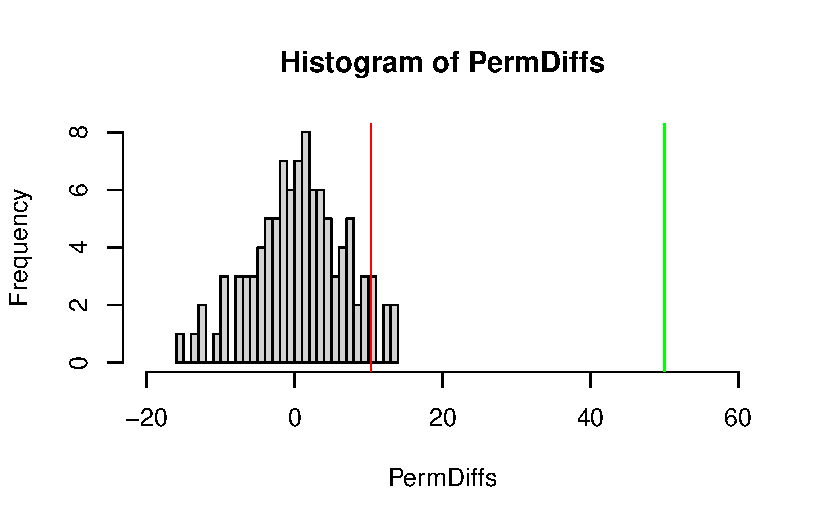
\includegraphics[keepaspectratio]{R_kurssi/Osa03_files/figure-pdf/unnamed-chunk-8-1.pdf}}

\begin{Shaded}
\begin{Highlighting}[]
\CommentTok{\#myös voidaan manuaalisesti etsiä kohta, jossa permutaatioiden keskiarvoero on sama, kuin todellinen }
  \CommentTok{\#   ryhmien ero, ja katsoa onko kuinka iso osa permutaatioista sen alle }
\CommentTok{\# sortataan permutaatiot sort() funktiolla }

\FunctionTok{sort}\NormalTok{(PermDiffs)}
\end{Highlighting}
\end{Shaded}

\begin{verbatim}
  [1] -15.72 -13.00 -12.52 -12.20 -10.68  -9.84  -9.56  -9.32  -7.68  -7.60
 [11]  -7.48  -6.36  -6.20  -6.12  -5.84  -5.48  -5.20  -4.44  -4.36  -4.32
 [21]  -4.12  -3.84  -3.52  -3.40  -3.16  -3.00  -2.96  -2.80  -2.76  -2.60
 [31]  -2.04  -1.88  -1.84  -1.68  -1.44  -1.36  -1.32  -1.28  -0.96  -0.76
 [41]  -0.48  -0.48  -0.40  -0.08   0.08   0.16   0.28   0.32   0.36   0.68
 [51]   0.72   1.08   1.20   1.36   1.36   1.64   1.68   1.84   1.96   2.52
 [61]   2.68   2.92   3.00   3.00   3.00   3.24   3.28   3.36   3.40   3.64
 [71]   3.80   4.24   4.28   4.32   4.64   5.00   5.52   5.60   5.76   6.16
 [81]   6.24   6.48   7.00   7.20   7.36   7.56   7.72   7.88   8.12   8.60
 [91]   9.20   9.32   9.96  10.12  10.32  10.84  12.16  12.24  13.72  13.72
\end{verbatim}

\begin{Shaded}
\begin{Highlighting}[]
\CommentTok{\# tässä tapauksessa kaikki permutaatioiden keskiarvoerot jäävät todellisen keskiarvoeron alle eli sen }
  \CommentTok{\# mukaan ero on hyvinkin merkitsevä }
  \CommentTok{\# sen vuoksi myöskään Viljamin tapa laskea p{-}arvo ei toimi, koska ei indeksistä ei tule yhtään osumaa}
  \CommentTok{\# toimii silloin, kun permutaatioista vähintään 1 on yli havaitun keskiarvoeron }
\CommentTok{\#p{-}arvon laskeminen }

\CommentTok{\#SortedDiffs \textless{}{-} sort(PermDiffs) }
\CommentTok{\#FirstIndex \textless{}{-} min(which( SortedDiffs \textgreater{} GrpDiff))}
\CommentTok{\#Pval \textless{}{-} 1 {-} FirstIndex/Nperms}


\CommentTok{\# geminin ehdottama tapa laskea p{-}arvo }

\CommentTok{\# sum() laskee TRUE{-}arvojen määrän (TRUE = 1, FALSE = 0)}
  \CommentTok{\# eli laskee niiden kertojen lukumäärän, kun permutaatioiden ero, on suurempi kuin havaittu ero }
\NormalTok{Osumat }\OtherTok{\textless{}{-}} \FunctionTok{sum}\NormalTok{(PermDiffs }\SpecialCharTok{\textgreater{}=}\NormalTok{ GrpDiff)}
\NormalTok{Pval }\OtherTok{\textless{}{-}}\NormalTok{ Osumat  }\SpecialCharTok{/}\NormalTok{ Nperms}

\CommentTok{\# gemini myös suositteli lisäämään 1 sekä osoittajaan, että nimittäjään, jolla vältetään}
\CommentTok{\#  tasan 0 p{-}arvo }
  \CommentTok{\# tasan 0 p{-}arvo on teoreettisesti mahdoton, koska alkuperäinen havainto on oikeasti yksi permutaatioista }

\NormalTok{Osumat }\OtherTok{\textless{}{-}} \FunctionTok{sum}\NormalTok{(PermDiffs }\SpecialCharTok{\textgreater{}=}\NormalTok{ GrpDiff)}
\NormalTok{Pval }\OtherTok{\textless{}{-}}\NormalTok{ (Osumat }\SpecialCharTok{+} \DecValTok{1}\NormalTok{)}\SpecialCharTok{/}\NormalTok{(Nperms }\SpecialCharTok{+} \DecValTok{1}\NormalTok{) }
\NormalTok{Pval}
\end{Highlighting}
\end{Shaded}

\begin{verbatim}
[1] 0.00990099
\end{verbatim}

\begin{Shaded}
\begin{Highlighting}[]
\CommentTok{\# t.test(arvot \textasciitilde{} ryhmä, data = aineisto)}

\FunctionTok{t.test}\NormalTok{(value }\SpecialCharTok{\textasciitilde{}}\NormalTok{ group, }\AttributeTok{data =}\NormalTok{ data) }
\end{Highlighting}
\end{Shaded}

\begin{verbatim}

    Welch Two Sample t-test

data:  value by group
t = -17.15, df = 98, p-value < 2.2e-16
alternative hypothesis: true difference in means between group 1 and group 2 is not equal to 0
95 percent confidence interval:
 -55.78567 -44.21433
sample estimates:
mean in group 1 mean in group 2 
           25.5            75.5 
\end{verbatim}

\begin{Shaded}
\begin{Highlighting}[]
\FunctionTok{t.test}\NormalTok{(group1, group2)}
\end{Highlighting}
\end{Shaded}

\begin{verbatim}

    Welch Two Sample t-test

data:  group1 and group2
t = -17.15, df = 98, p-value < 2.2e-16
alternative hypothesis: true difference in means is not equal to 0
95 percent confidence interval:
 -55.78567 -44.21433
sample estimates:
mean of x mean of y 
     25.5      75.5 
\end{verbatim}

\chapter{Osa 4 - Tekoälyn käyttö ohjelmoinnin
tukena}\label{osa-4---tekouxe4lyn-kuxe4yttuxf6-ohjelmoinnin-tukena}

Tässä osassa asiaa luennoista, joissa käsitellään tekoälyn käyttöä
ohjelmoinnissa. Lisäksi osan 4 tehtävien muistiinpanot.

\section{Ohjelmointia tekoälyn avustamana, luento
26.03}\label{ohjelmointia-tekouxe4lyn-avustamana-luento-26.03}

\subsection{AI:n käyttö}\label{ain-kuxe4yttuxf6}

\begin{itemize}
\item
  koodin kirjoittaminen
\item
  debuggaaminen ja koodin arviointi
\item
  koodin selittäminen
\item
  koodin optimointi
\end{itemize}

\subsection{AI-työkaluja}\label{ai-tyuxf6kaluja}

\begin{itemize}
\item
  Yliopiston suosittelemat (tietoturvan vuoksi, etenkin currechat)

  \begin{itemize}
  \item
    Currechat
  \item
    Copilot
  \end{itemize}
\end{itemize}

\subsection{R-koodin tuottaminen}\label{r-koodin-tuottaminen}

\begin{itemize}
\item
  yksityiskohtaiset promptit
\item
  englanti voi toimia paremmin kuin suomi
\item
  tarkat tilastolliset termit

  \begin{itemize}
  \tightlist
  \item
    esim. reverse coding items/variables
  \end{itemize}
\item
  kerro mitkä ovat data framen/tiedoston nimi \& kerro muutttujien nimet

  \begin{itemize}
  \tightlist
  \item
    skripti toimii suoraan
  \end{itemize}
\item
  Ole tarkkana, että skripti tekee kaiken minkä pyydät
\item
  ole skeptinen, AI tekee oikopolkuja
\item
  jos vähänkin epäilet, niin pyydä tarkennusta
\item
  Kehitä skriptiä iteratiivisesti -- pyydä lisää ominaisuuksia /
  tarkennuksia; pyydä vaihtoehtoisia tapoja ratkaista asia
\item
  Jos virhe, syötä se AI:lle ja pyydä korjaamaan
\item
  Tee tehtävät huolellisesti

  \begin{itemize}
  \tightlist
  \item
    jos et itse ymmärrä niin todnäk ovat virheellisiä
  \end{itemize}
\end{itemize}

\subsection{Skriptien optimointi ja
organisointi}\label{skriptien-optimointi-ja-organisointi}

\begin{itemize}
\item
  For-loop voi olla hidas, löytyy muitakin mahdollisia toteutuksia esim.
  replicate/apply

  \begin{itemize}
  \item
    ei vakava ongelma, koska laskentatehoa riittää
  \item
    kannattaa tehdä skriptejä, joita itse ymmärtää
  \end{itemize}
\item
  kommentoi tarkasti
\item
  Tee funktioita

  \begin{itemize}
  \item
    silloin voi soveltaa muihinkin aineistoihin
  \item
    automatisoi mahd. paljon
  \end{itemize}
\item
  esim. viimeistele visualisoinnit
\item
  kerro tekoälylle suoraan muuttujien nimet, data-frame nimi yms. niin
  koodi toimii suoraan
\item
  Tee erillisiä skriptejä

  \begin{itemize}
  \item
    yksi, joka tekee preprosessoinnin
  \item
    toinen, joka tekee tilastoanalyysit
  \item
    kolmas, joka tekee visualisoinnit
  \item
    ja pääskripti, jossa tehdään kaikki/tarvittavat vaiheet oikeassa
    järjestyksessä
  \end{itemize}
\end{itemize}

Salmela (2026)

\section{PreProsessointi funktio
tehtävä}\label{preprosessointi-funktio-tehtuxe4vuxe4}

Tehtävänanto:

\begin{quote}
\emph{Tee funktio, jolle voi antaa 5 argumenttia: data-kehikon,
muuttujat joita ei käännetä, muuttujat jotka käännetään (reverse
coding), muuttujien minimin ja maksimin.}

\emph{Funktio sitten muuntaa asteikon ulkopuolella olevat arvot
puuttuviksi havainnoiksi, laskee summamuuttujan, tarkistaa poikkeavat
havainnot, tekee tilastotestin summamuuttujan
normaalijakautuneisuudelle, raportoi sen tuloksen selväsanaisesti (onko
vai ei, mikä oli tulos), piirtää kuvan jossa kolme kuvaa vierekkäin:
summamuuttujan histogrammi, summamuuttujan Q-Q plotin, summammuuttujaa
vastaavan simuloidun normaalijakauman Q-Q plotin.}

\emph{Sovella funktiota HSQ-aineistoon (Humor Styles Questionnaire)}

\emph{palauta 2 tiedostoa, R-skripti ja pdf, jossa neljän
HSQ-summamuuttujan jakaumat}
\end{quote}

Tehtävän ratkaisu:

\begin{Shaded}
\begin{Highlighting}[]
\CommentTok{\#ladataan data }
\FunctionTok{library}\NormalTok{(readr)}
\FunctionTok{library}\NormalTok{(dplyr)}
\FunctionTok{library}\NormalTok{(ggplot2)}
\FunctionTok{library}\NormalTok{(patchwork)}
\NormalTok{HSQdata }\OtherTok{\textless{}{-}} \FunctionTok{read\_csv}\NormalTok{(}\StringTok{"HSQdata.csv"}\NormalTok{)}

\CommentTok{\# HSQ käännettävät muuttujat \textquotesingle{}Q1\textquotesingle{}, \textquotesingle{}Q7\textquotesingle{}, \textquotesingle{}Q9\textquotesingle{}, \textquotesingle{}Q15\textquotesingle{}, \textquotesingle{}Q16\textquotesingle{}, \textquotesingle{}Q17\textquotesingle{}, \textquotesingle{}Q22\textquotesingle{}, \textquotesingle{}Q23\textquotesingle{}, \textquotesingle{}Q25\textquotesingle{}, \textquotesingle{}Q29\textquotesingle{}, \textquotesingle{}Q31, }


\NormalTok{affiliative }\OtherTok{\textless{}{-}} \FunctionTok{c}\NormalTok{(}\StringTok{"Q1"}\NormalTok{, }\StringTok{"Q5"}\NormalTok{, }\StringTok{"Q9"}\NormalTok{, }\StringTok{"Q13"}\NormalTok{, }\StringTok{"Q17"}\NormalTok{, }\StringTok{"Q21"}\NormalTok{, }\StringTok{"Q25"}\NormalTok{, }\StringTok{"Q29"}\NormalTok{)}

\NormalTok{selfenhancing }\OtherTok{\textless{}{-}} \FunctionTok{c}\NormalTok{(}\StringTok{"Q2"}\NormalTok{, }\StringTok{"Q6"}\NormalTok{, }\StringTok{"Q10"}\NormalTok{,}\StringTok{"Q14"}\NormalTok{, }\StringTok{"Q18"}\NormalTok{, }\StringTok{"Q22"}\NormalTok{,}\StringTok{"Q26"}\NormalTok{, }\StringTok{"Q30"}\NormalTok{)}

\NormalTok{aggressive }\OtherTok{\textless{}{-}} \FunctionTok{c}\NormalTok{(}\StringTok{"Q3"}\NormalTok{, }\StringTok{"Q7"}\NormalTok{, }\StringTok{"Q11"}\NormalTok{, }\StringTok{"Q15"}\NormalTok{, }\StringTok{"Q19"}\NormalTok{, }\StringTok{"Q23"}\NormalTok{, }\StringTok{"Q27"}\NormalTok{, }\StringTok{"Q31"}\NormalTok{) }

\NormalTok{selfdefeating }\OtherTok{\textless{}{-}} \FunctionTok{c}\NormalTok{(}\StringTok{"Q4"}\NormalTok{, }\StringTok{"Q8"}\NormalTok{, }\StringTok{"Q12"}\NormalTok{, }\StringTok{"Q16"}\NormalTok{, }\StringTok{"Q20"}\NormalTok{, }\StringTok{"Q24"}\NormalTok{, }\StringTok{"Q28"}\NormalTok{, }\StringTok{"Q32"}\NormalTok{)}



\NormalTok{PreProsFunktio}\OtherTok{\textless{}{-}} \ControlFlowTok{function}\NormalTok{(data, }\AttributeTok{variables =} \ConstantTok{NULL}\NormalTok{, }\AttributeTok{r\_variables =} \ConstantTok{NULL}\NormalTok{,  }\AttributeTok{min =} \DecValTok{1}\NormalTok{, }\AttributeTok{max =} \DecValTok{5}\NormalTok{, SumMuut, }\AttributeTok{Otsikko =} \FunctionTok{deparse}\NormalTok{(}\FunctionTok{substitute}\NormalTok{(SumMuut)))\{}
  
  \CommentTok{\# r\_variables kohtaan sarakkeet, jotka käännetään}
  \CommentTok{\# variables kohtaan muut }
  
  
  \CommentTok{\# Tarkistetaan, onko r\_variables annettu ja onko siinä sisältöä}
  \ControlFlowTok{if}\NormalTok{ (}\SpecialCharTok{!}\FunctionTok{is.null}\NormalTok{(r\_variables) }\SpecialCharTok{\&\&} \FunctionTok{length}\NormalTok{(r\_variables) }\SpecialCharTok{\textgreater{}} \DecValTok{0}\NormalTok{)\{}
    
\NormalTok{    data[, r\_variables] }\OtherTok{\textless{}{-}}\NormalTok{ (max }\SpecialCharTok{+}\NormalTok{ min) }\SpecialCharTok{{-}}\NormalTok{ data[, r\_variables]}
    \FunctionTok{message}\NormalTok{(}\StringTok{"Käänteiset muuttujat käännetty."}\NormalTok{)}
\NormalTok{  \} }\ControlFlowTok{else}\NormalTok{ \{}
    \FunctionTok{message}\NormalTok{(}\StringTok{"Ei käännettäviä muuttujia, ohitetaan kääntö."}\NormalTok{)}
\NormalTok{  \}}
  
    
  
  \CommentTok{\#merkataan asteikon ulkopuoliset arvot puuttuviksi }
  \CommentTok{\# katsotaan mitkä arvot ovat liian pieniä TAI liian suuria}
\NormalTok{  virheelliset }\OtherTok{\textless{}{-}}\NormalTok{ data }\SpecialCharTok{\textless{}}\NormalTok{ min }\SpecialCharTok{|}\NormalTok{ data }\SpecialCharTok{\textgreater{}}\NormalTok{ max}
  
  \CommentTok{\# Korvataan nämä kohdat NA{-}arvolla}
\NormalTok{  data[virheelliset] }\OtherTok{\textless{}{-}} \ConstantTok{NA}
  \FunctionTok{message}\NormalTok{(}\StringTok{"Asteikon ulkopuoliset arvot poistettu"}\NormalTok{)}
  \CommentTok{\# tarkistetaan poikkeavat havainnot MAD{-}kriteerillä }
  
  \CommentTok{\# luodaan datafreimistä vektori, johon voidaan käyttääm mad() ja median() funktioita}
  
\NormalTok{  numarvot }\OtherTok{\textless{}{-}} \FunctionTok{as.numeric}\NormalTok{(}\FunctionTok{unlist}\NormalTok{(data[ ,}\DecValTok{1}\SpecialCharTok{:}\DecValTok{32}\NormalTok{]))}
  
  
\NormalTok{  mad\_value }\OtherTok{\textless{}{-}} \FunctionTok{mad}\NormalTok{(}\FunctionTok{na.omit}\NormalTok{(numarvot)) }
\NormalTok{  median\_value }\OtherTok{\textless{}{-}} \FunctionTok{median}\NormalTok{(}\FunctionTok{na.omit}\NormalTok{(numarvot))}
  
  \CommentTok{\#Jos poikkeava havainto niin ilmoitetaan löytyi poikkeavia havaintoja, jos ei niin päinvastoin}
  
  
\NormalTok{  threshold }\OtherTok{\textless{}{-}} \DecValTok{3} \SpecialCharTok{*}\NormalTok{ mad\_value}
  
\NormalTok{  filtered\_data }\OtherTok{\textless{}{-}}\NormalTok{ data[}\FunctionTok{abs}\NormalTok{(data }\SpecialCharTok{{-}}\NormalTok{ median\_value) }\SpecialCharTok{\textgreater{}=}\NormalTok{ threshold]}
  
  \ControlFlowTok{if}\NormalTok{(}\FunctionTok{length}\NormalTok{(filtered\_data) }\SpecialCharTok{\textgreater{}} \DecValTok{0}\NormalTok{)\{}
    \FunctionTok{message}\NormalTok{(}\StringTok{"Löytyi poikkeavia arvoja"}\NormalTok{)}
\NormalTok{  \} }\ControlFlowTok{else}\NormalTok{ \{}
    \FunctionTok{message}\NormalTok{(}\StringTok{"Ei poikkeavia arvoja"}\NormalTok{)\}}
  
  \CommentTok{\#tehdään summamuuttujat eri huumorityypeille}
  
\NormalTok{  SummaMuuttuja }\OtherTok{\textless{}{-}} \FunctionTok{rowMeans}\NormalTok{(data[ ,SumMuut], }\AttributeTok{na.rm =} \ConstantTok{TRUE}\NormalTok{)}
  
\NormalTok{  data}\SpecialCharTok{$}\NormalTok{SummaMuuttuja }\OtherTok{\textless{}{-}}\NormalTok{ SummaMuuttuja}
  
\NormalTok{ntesti }\OtherTok{\textless{}{-}} \FunctionTok{shapiro.test}\NormalTok{(}\FunctionTok{na.omit}\NormalTok{(SummaMuuttuja))}

\NormalTok{p\_arvo }\OtherTok{\textless{}{-}} \FunctionTok{as.numeric}\NormalTok{(ntesti) }

\ControlFlowTok{if}\NormalTok{(p\_arvo[}\DecValTok{1}\NormalTok{] }\SpecialCharTok{\textless{}} \FloatTok{0.05}\NormalTok{)\{}
  \FunctionTok{message}\NormalTok{(}\StringTok{"Shapiro{-}wilk testin p \textless{} 0.05, Summamuuttuja ei siis ole normaalisti jakautunut"}\NormalTok{)}
\NormalTok{\}}\ControlFlowTok{else}\NormalTok{ \{}
  \FunctionTok{message}\NormalTok{(}\StringTok{"Shapiro{-}wilk testin p \textgreater{} 0.05, Summamuuttuja on normaalisti jakautunut"}\NormalTok{)}
\NormalTok{\}}

\CommentTok{\# Summamuuttujaa vastaava simuloitu normaalijakauma }

\FunctionTok{set.seed}\NormalTok{(}\DecValTok{123}\NormalTok{)}
\NormalTok{SimuloituJakauma }\OtherTok{\textless{}{-}} \FunctionTok{rnorm}\NormalTok{(}\FunctionTok{length}\NormalTok{(}\FunctionTok{na.omit}\NormalTok{(SummaMuuttuja)), }\FunctionTok{mean}\NormalTok{(SummaMuuttuja, }\AttributeTok{na.rm =} \ConstantTok{TRUE}\NormalTok{), }\FunctionTok{sd}\NormalTok{(SummaMuuttuja, }\AttributeTok{na.rm =} \ConstantTok{TRUE}\NormalTok{))}
  
\NormalTok{Simdata }\OtherTok{\textless{}{-}} \FunctionTok{data.frame}\NormalTok{(SimuloituJakauma)}

\CommentTok{\# luodaan muuuttuja, johon tulee vain annetun summamuuttujan nimi}
\NormalTok{Labs }\OtherTok{\textless{}{-}} \FunctionTok{deparse}\NormalTok{(}\FunctionTok{substitute}\NormalTok{(SumMuut))}
  
\CommentTok{\# Piirretään kuvaajat ggplotilla, qqplot, simuloidun jakauman qqplot ja histogrammi }
\NormalTok{ p1 }\OtherTok{\textless{}{-}} \FunctionTok{ggplot}\NormalTok{(data, }\FunctionTok{aes}\NormalTok{(}\AttributeTok{sample =}\NormalTok{ SummaMuuttuja )) }\SpecialCharTok{+}
    \FunctionTok{geom\_qq}\NormalTok{() }\SpecialCharTok{+}
    \FunctionTok{geom\_qq\_line}\NormalTok{(}\AttributeTok{color =} \StringTok{"red"}\NormalTok{) }\SpecialCharTok{+}
    \FunctionTok{labs}\NormalTok{(}\AttributeTok{title =} \FunctionTok{paste}\NormalTok{(Otsikko, }\StringTok{"QQ{-}plot"}\NormalTok{)) }\SpecialCharTok{+}
    \FunctionTok{theme\_minimal}\NormalTok{()}
 
\NormalTok{ p2 }\OtherTok{\textless{}{-}} \FunctionTok{ggplot}\NormalTok{(Simdata, }\FunctionTok{aes}\NormalTok{( }\AttributeTok{sample =}\NormalTok{ SimuloituJakauma )) }\SpecialCharTok{+} 
   \FunctionTok{geom\_qq}\NormalTok{() }\SpecialCharTok{+}
   \FunctionTok{geom\_qq\_line}\NormalTok{(}\AttributeTok{color =} \StringTok{"red"}\NormalTok{) }\SpecialCharTok{+}
   \FunctionTok{labs}\NormalTok{(}\AttributeTok{title =} \StringTok{"Simuloidun jakauman QQ{-}plot"}\NormalTok{) }\SpecialCharTok{+}
   \FunctionTok{theme\_minimal}\NormalTok{()}
 
  
  
\NormalTok{ p3 }\OtherTok{\textless{}{-}} \FunctionTok{ggplot}\NormalTok{(data, }\FunctionTok{aes}\NormalTok{( }\AttributeTok{x =}\NormalTok{ SummaMuuttuja)) }\SpecialCharTok{+} 
           \FunctionTok{geom\_histogram}\NormalTok{(}\AttributeTok{fill =} \StringTok{"lightblue"}\NormalTok{, }\AttributeTok{color =} \StringTok{"black"}\NormalTok{, }\AttributeTok{bins =} \DecValTok{10}\NormalTok{) }\SpecialCharTok{+}
           \FunctionTok{labs}\NormalTok{(}\AttributeTok{title =} \FunctionTok{paste}\NormalTok{(Otsikko, }\StringTok{"jakauma"}\NormalTok{), }\AttributeTok{x =} \StringTok{"Keskiarvo"}\NormalTok{, }\AttributeTok{y =} \StringTok{"Frekvenssi"}\NormalTok{) }\SpecialCharTok{+}
           \FunctionTok{theme\_minimal}\NormalTok{()}
  \FunctionTok{print}\NormalTok{(p1 }\SpecialCharTok{+}\NormalTok{ p2 }\SpecialCharTok{+}\NormalTok{ p3)}
  
\NormalTok{\}}




\FunctionTok{PreProsFunktio}\NormalTok{(HSQdata,  , }\FunctionTok{c}\NormalTok{(}\StringTok{"Q1"}\NormalTok{, }\StringTok{"Q7"}\NormalTok{, }\StringTok{"Q9"}\NormalTok{, }\StringTok{"Q15"}\NormalTok{, }\StringTok{"Q16"}\NormalTok{, }\StringTok{"Q17"}\NormalTok{, }\StringTok{"Q22"}\NormalTok{, }\StringTok{"Q23"}\NormalTok{, }\StringTok{"Q25"}\NormalTok{, }\StringTok{"Q29"}\NormalTok{, }\StringTok{"Q31"}\NormalTok{), }\DecValTok{1}\NormalTok{, }\DecValTok{5}\NormalTok{, selfenhancing)}


\CommentTok{\#Piirretään kuvaajat yhteeen pdf tiedostoon }

\CommentTok{\# luodaan lista, johon on tallennettu summamuuttujat }
\NormalTok{kaikki\_tyylit }\OtherTok{\textless{}{-}} \FunctionTok{list}\NormalTok{(}
  \AttributeTok{affiliative =}\NormalTok{ affiliative, }
  \AttributeTok{selfenhancing =}\NormalTok{ selfenhancing, }
  \AttributeTok{aggressive =}\NormalTok{ aggressive, }
  \AttributeTok{selfdefeating =}\NormalTok{ selfdefeating)}

\CommentTok{\# while komento varmistaa, ettei pdf:n kirjoitus ole jäänyt auki aiemmin }
\ControlFlowTok{while}\NormalTok{ (}\SpecialCharTok{!}\FunctionTok{is.null}\NormalTok{(}\FunctionTok{dev.list}\NormalTok{())) }\FunctionTok{dev.off}\NormalTok{()}

\CommentTok{\#pdf komento avaa pdf:n kirjoituksen }
\FunctionTok{pdf}\NormalTok{(}\StringTok{"Summamuuttujien\_kuvaajat.pdf"}\NormalTok{, }\AttributeTok{width =} \DecValTok{14}\NormalTok{, }\AttributeTok{height =} \DecValTok{5}\NormalTok{)}

\FunctionTok{try}\NormalTok{(\{}
  \ControlFlowTok{for}\NormalTok{ (i }\ControlFlowTok{in} \DecValTok{1}\SpecialCharTok{:}\FunctionTok{length}\NormalTok{(kaikki\_tyylit)) \{}
  

  \CommentTok{\# napataan listasta yksi huumorityyli kerrallaan}
\NormalTok{  nykyinen\_setti }\OtherTok{\textless{}{-}}\NormalTok{ kaikki\_tyylit[[i]]}
  
  
  \FunctionTok{PreProsFunktio}\NormalTok{(}\AttributeTok{data =}\NormalTok{ HSQdata, ,}
                 \FunctionTok{c}\NormalTok{(}\StringTok{"Q1"}\NormalTok{, }\StringTok{"Q7"}\NormalTok{, }\StringTok{"Q9"}\NormalTok{, }\StringTok{"Q15"}\NormalTok{, }\StringTok{"Q16"}\NormalTok{, }\StringTok{"Q17"}\NormalTok{, }\StringTok{"Q22"}\NormalTok{, }\StringTok{"Q23"}\NormalTok{, }\StringTok{"Q25"}\NormalTok{, }\StringTok{"Q29"}\NormalTok{, }\StringTok{"Q31"}\NormalTok{), }
                 \AttributeTok{min =} \DecValTok{1}\NormalTok{, }
                 \AttributeTok{max =} \DecValTok{5}\NormalTok{, }
                 \AttributeTok{SumMuut =}\NormalTok{ nykyinen\_setti,}
                 \AttributeTok{Otsikko =} \FunctionTok{names}\NormalTok{(kaikki\_tyylit)[i])}
\NormalTok{  \}}
\NormalTok{\})}
\FunctionTok{dev.off}\NormalTok{()}
\CommentTok{\# Tämä sulkee pdf:n kirjoittamisen }
\end{Highlighting}
\end{Shaded}

unlist()

\begin{itemize}
\item
  muuntaa datan matriisi tai dataframe muodosta takaisin vektoriksi
\item
  esim.
\end{itemize}

\begin{Shaded}
\begin{Highlighting}[]
\NormalTok{ numarvot }\OtherTok{\textless{}{-}} \FunctionTok{as.numeric}\NormalTok{(}\FunctionTok{unlist}\NormalTok{(data[ ,}\DecValTok{1}\SpecialCharTok{:}\DecValTok{32}\NormalTok{]))}
\end{Highlighting}
\end{Shaded}

\begin{itemize}
\item
  unlist() komennolla pois kehikkomuodosta ja as.numeric() komennolla
  varmistetaan, että tallentuu numeerisena
\item
  numarvot \textless- as.numeric(unlist(data{[} ,1:32{]}))
\end{itemize}

! huutomerkki tarkoittaa loogista ei operaattoria, \&\& ja if
lausekkeessa

\begin{itemize}
\item
  esim.

\begin{Shaded}
\begin{Highlighting}[]
\ControlFlowTok{if}\NormalTok{ (}\SpecialCharTok{!}\FunctionTok{is.null}\NormalTok{(r\_variables) }\SpecialCharTok{\&\&} \FunctionTok{length}\NormalTok{(r\_variables) }\SpecialCharTok{\textgreater{}} \DecValTok{0}\NormalTok{)}
\end{Highlighting}
\end{Shaded}
\item
  huutomerkki tarkoittaa komennossa !is.null(), sitä että kun
  r\_variables muuttuja ei ole tyhjä niin ehto täyttyy --\textgreater{}
  ts. is not null
\item
  \&\& merkki tarkoittaa JA eli sitä, että molempien ehtojen täytyy
  täyttyä, jotta if lausekkeen ehdot toteutuvat

  \begin{itemize}
  \tightlist
  \item
    kahta \&\& merkkiä käytetään lähinnä if lausekkeissa, muualla yhtä
    \& merkki
  \end{itemize}
\item
  Tai puolestaan merkitään \textbar{} pystyviivalla, if lausekkeessa
  kannattaa käyttää kahta \textbar\textbar{} ja muualla yksi
  \textbar~riittää

  \begin{itemize}
  \tightlist
  \item
    eli merkitsee if lausekkeessa sitä, että jomman kumman ehdon
    täyttyminen riittää
  \end{itemize}
\end{itemize}

\section{Visualisointitehtävä}\label{visualisointitehtuxe4vuxe4}

Tehtävänanto :

\begin{quote}
\emph{Oheisessa data-setissä on tutkittu lääketieteen opiskelijoiden
visuaalisen asiantuntijuuden (professional vision/perceptual learning)
kehittymistä osana dermatologian kurssia. Diagnoosien erottelu-kokeet
tehtiin kurssin aluksi, keskellä ja lopuksi (Session:1-3, pre-mid-post).
Oppimista mitattiin kolmella muuttujalla: \%-oikein, reaktioaika,
confidence-rating,}

\emph{Tee R-skripti, joka visualisoi tulokset, eli oppimisen/muutoksen
kurssin aikana (pre-mid-post) kolmen outcome muuttujan suhteen.}

\emph{Tutki dataa lisää, kokeessa oli 47 eri diagnoosia. Mitkä
diagnoosit käyttäytyvät samanlaisesti? Klusteroi diagnooseja yhteen ja
visualisoi oppiminen. Missä diagnooseissa opiskelijat tekivät eniten
virheitä? Luokittele vaikeat/helpot diagnoosit ja visualisoi oppiminen.
Ideoita/esimerkkejä voi katsoa artikkeleista (data osittain eri) tai
keksiä ihan uusia tapoja.}

\emph{Palauta R-skripti ja erikseen kuvat pdf:nä.}
\end{quote}

\begin{Shaded}
\begin{Highlighting}[]
\CommentTok{\# Skripti tulostaa PDF tiedoston, jossa on kuvaajat kaikille outcome muuttujille sessioittain,}
  \CommentTok{\# kuvaus siitä miten diagnooseja on jaoteltu klustereihin ja kuvaajat oppimisen kehityksestä }
    \CommentTok{\# klustereittain}

\CommentTok{\# oppimisen muutokset kurssin aikana pre{-}mid{-}post }
\CommentTok{\# 47 eri diagnoosia, mitkä käyttäytyvät samanlaisesti}

\CommentTok{\# klusteroi diagnooseja yhteen ja visualisoi oppiminen }
\CommentTok{\# missä tehtiin eniten virheitä}
\CommentTok{\# luokittelet vaikeat ja helpot diagnoosit ja visualisoi oppiminen }

\CommentTok{\# "Correct"         \%{-}correct}
\CommentTok{\# "respRT"          decision time, ms}
\CommentTok{\# "Confidence"      confidence rating, 1{-}5}

\CommentTok{\# Jokaisella on 47 vastausta per sessio ja 2 eri moduulia = 282 vastausta}

\FunctionTok{library}\NormalTok{(gridExtra)}
\FunctionTok{library}\NormalTok{(grid)}
\FunctionTok{library}\NormalTok{(readr)}
\FunctionTok{library}\NormalTok{(ggplot2)}
\FunctionTok{library}\NormalTok{(patchwork)}

\NormalTok{PerceptualLearnData }\OtherTok{\textless{}{-}} \FunctionTok{read\_csv}\NormalTok{(}\StringTok{"data/PerceptualLearn/PerceptualLearnData.csv"}\NormalTok{)}
\CommentTok{\#haetaan data}





\NormalTok{oikeinbydiagnoosi }\OtherTok{\textless{}{-}} \FunctionTok{aggregate}\NormalTok{(Correct }\SpecialCharTok{\textasciitilde{}}\NormalTok{ SelectedDiag, }\AttributeTok{data =}\NormalTok{ PerceptualLearnData, }\AttributeTok{FUN =}\NormalTok{ mean)}
\CommentTok{\#}


\NormalTok{keskikvartiiliväli }\OtherTok{\textless{}{-}}\NormalTok{ oikeinbydiagnoosi}\SpecialCharTok{$}\NormalTok{SelectedDiag[oikeinbydiagnoosi}\SpecialCharTok{$}\NormalTok{Correct }\SpecialCharTok{\textgreater{}} \FloatTok{0.763} \SpecialCharTok{\&}\NormalTok{ oikeinbydiagnoosi}\SpecialCharTok{$}\NormalTok{Correct }\SpecialCharTok{\textless{}} \FloatTok{0.8613}\NormalTok{]}
\NormalTok{IQRtekstinä }\OtherTok{\textless{}{-}} \FunctionTok{paste}\NormalTok{(keskikvartiiliväli, }\AttributeTok{collapse =} \StringTok{", "}\NormalTok{)}

\NormalTok{vaikeimmat }\OtherTok{\textless{}{-}}\NormalTok{ oikeinbydiagnoosi}\SpecialCharTok{$}\NormalTok{SelectedDiag[oikeinbydiagnoosi}\SpecialCharTok{$}\NormalTok{Correct }\SpecialCharTok{\textless{}} \FloatTok{0.6884807}\NormalTok{]}
\NormalTok{vaikeimmatTekst }\OtherTok{\textless{}{-}} \FunctionTok{paste}\NormalTok{(vaikeimmat, }\AttributeTok{collapse =} \StringTok{","}\NormalTok{) }

\NormalTok{helpoimmat }\OtherTok{\textless{}{-}}\NormalTok{ oikeinbydiagnoosi}\SpecialCharTok{$}\NormalTok{SelectedDiag[oikeinbydiagnoosi}\SpecialCharTok{$}\NormalTok{Correct }\SpecialCharTok{\textgreater{}} \FloatTok{0.9159686}\NormalTok{]}
\NormalTok{helpoimmatTekst }\OtherTok{\textless{}{-}} \FunctionTok{paste}\NormalTok{(helpoimmat, }\AttributeTok{collapse =} \StringTok{","}\NormalTok{) }

\FunctionTok{quantile}\NormalTok{(oikeinbydiagnoosi}\SpecialCharTok{$}\NormalTok{Correct, }\AttributeTok{probs =} \FunctionTok{seq}\NormalTok{(}\DecValTok{0}\NormalTok{, }\DecValTok{1}\NormalTok{, }\FloatTok{0.1}\NormalTok{))}

\CommentTok{\# 10 persentiili = 68,85 \% }
\CommentTok{\# 90 persentiili = 91,60 \% }
\CommentTok{\# keskikvartiiliväli =  76,30 \% \textless{} oikein \textless{} 86,13 \% }

\CommentTok{\# havainnollistetaan vaikeimpien diagnoosien kehitys sessioittain}
  \CommentTok{\# haetaan selectedDiag sarakkeesta vain tietyt diagnoosit ja katsotaan miten ne meni oikein per sessio}
    \CommentTok{\# se onnistuu subset() funktiolla }

\NormalTok{vaikeat }\OtherTok{\textless{}{-}} \FunctionTok{subset}\NormalTok{(PerceptualLearnData, SelectedDiag }\SpecialCharTok{\%in\%}\NormalTok{ vaikeimmat)}
\NormalTok{kehitysVaikeat }\OtherTok{\textless{}{-}} \FunctionTok{aggregate}\NormalTok{(Correct }\SpecialCharTok{\textasciitilde{}}\NormalTok{ Session, vaikeat, }\AttributeTok{FUN =}\NormalTok{ mean)}

\CommentTok{\# tehdään sama helpoimmille ja keskikvartiilivälille }

\NormalTok{helpot }\OtherTok{\textless{}{-}} \FunctionTok{subset}\NormalTok{(PerceptualLearnData, SelectedDiag }\SpecialCharTok{\%in\%}\NormalTok{ helpoimmat)}
\NormalTok{kehitysHelpot }\OtherTok{\textless{}{-}} \FunctionTok{aggregate}\NormalTok{(Correct }\SpecialCharTok{\textasciitilde{}}\NormalTok{ Session, helpot, }\AttributeTok{FUN =}\NormalTok{ mean)}

\NormalTok{keski }\OtherTok{\textless{}{-}} \FunctionTok{subset}\NormalTok{(PerceptualLearnData, SelectedDiag }\SpecialCharTok{\%in\%}\NormalTok{ keskikvartiiliväli)}
\NormalTok{kehitysKeski }\OtherTok{\textless{}{-}} \FunctionTok{aggregate}\NormalTok{(Correct }\SpecialCharTok{\textasciitilde{}}\NormalTok{ Session, }\AttributeTok{data =}\NormalTok{ keski, }\AttributeTok{FUN =}\NormalTok{ mean)}


\FunctionTok{print}\NormalTok{(}\FunctionTok{ggplot}\NormalTok{(PerceptualLearnData, }\FunctionTok{aes}\NormalTok{(}\AttributeTok{x =} \FunctionTok{as.factor}\NormalTok{(SelectedDiag), }\AttributeTok{y =}\NormalTok{ Correct)) }\SpecialCharTok{+}
  \CommentTok{\# Piirretään keskiarvopylväät}
  \FunctionTok{stat\_summary}\NormalTok{(}\AttributeTok{fun =} \StringTok{"mean"}\NormalTok{, }\AttributeTok{geom =} \StringTok{"bar"}\NormalTok{, }\AttributeTok{color =} \StringTok{"black"}\NormalTok{, }\AttributeTok{width =} \FloatTok{0.5}\NormalTok{, }\AttributeTok{na.rm =} \ConstantTok{TRUE}\NormalTok{) }\SpecialCharTok{+}
  \CommentTok{\# Lisätään virhejanat (Standard Error)}
  \FunctionTok{stat\_summary}\NormalTok{(}\AttributeTok{fun.data =} \StringTok{"mean\_se"}\NormalTok{, }\AttributeTok{geom =} \StringTok{"errorbar"}\NormalTok{,}\AttributeTok{color =} \StringTok{"red"}\NormalTok{,  }\AttributeTok{width =} \FloatTok{0.3}\NormalTok{,}\AttributeTok{na.rm =} \ConstantTok{TRUE}\NormalTok{) }\SpecialCharTok{+}
  
  \FunctionTok{labs}\NormalTok{(}\AttributeTok{title =} \StringTok{"Mittaustulokset sessioittain"}\NormalTok{,}
       \AttributeTok{x =} \StringTok{"diagnoosi"}\NormalTok{,}
       \AttributeTok{y =} \StringTok{"Osuus vastauksista oikein"}\NormalTok{) }\SpecialCharTok{+}
  \FunctionTok{theme\_minimal}\NormalTok{())}


\CommentTok{\#  Määritellään sarakkeet, jotka halutaan y{-}akselille}
\NormalTok{y\_muuttujat }\OtherTok{\textless{}{-}} \FunctionTok{c}\NormalTok{(}\StringTok{"respRT"}\NormalTok{, }\StringTok{"Correct"}\NormalTok{, }\StringTok{"Confidence"}\NormalTok{) }\CommentTok{\# Vaihda nämä omiin sarakkeisiisi}


\CommentTok{\#  Suljetaan mahdolliset aiemmat jumiutuneet PDF{-}yhteydet}
\ControlFlowTok{while}\NormalTok{(}\SpecialCharTok{!}\FunctionTok{is.null}\NormalTok{(}\FunctionTok{dev.list}\NormalTok{())) }\FunctionTok{dev.off}\NormalTok{()}

\CommentTok{\#  Avataan PDF:n kirjoitus }
\FunctionTok{pdf}\NormalTok{(}\StringTok{"VisualisointiDiagnoosiTeht.pdf"}\NormalTok{, }\AttributeTok{width =} \DecValTok{8}\NormalTok{, }\AttributeTok{height =} \DecValTok{6}\NormalTok{)}

\NormalTok{kuvaaja\_lista }\OtherTok{\textless{}{-}} \FunctionTok{list}\NormalTok{()}

\CommentTok{\# for{-}looppi, joka piirtää kuvaajat }
\ControlFlowTok{for}\NormalTok{ (i }\ControlFlowTok{in}\NormalTok{ y\_muuttujat) \{}
  
\NormalTok{  p }\OtherTok{\textless{}{-}} \FunctionTok{ggplot}\NormalTok{(PerceptualLearnData, }\FunctionTok{aes}\NormalTok{(}\AttributeTok{x =} \FunctionTok{as.factor}\NormalTok{(Session), }\AttributeTok{y =}\NormalTok{ .data[[i]], }\AttributeTok{fill =}\NormalTok{ Session)) }\SpecialCharTok{+}
    \FunctionTok{stat\_summary}\NormalTok{(}\AttributeTok{fun =} \StringTok{"mean"}\NormalTok{, }\AttributeTok{geom =} \StringTok{"bar"}\NormalTok{, }\AttributeTok{color =} \StringTok{"black"}\NormalTok{, }\AttributeTok{width =} \FloatTok{0.8}\NormalTok{, }\AttributeTok{na.rm =} \ConstantTok{TRUE}\NormalTok{) }\SpecialCharTok{+}
    \FunctionTok{stat\_summary}\NormalTok{(}\AttributeTok{fun.data =} \StringTok{"mean\_se"}\NormalTok{, }\AttributeTok{geom =} \StringTok{"errorbar"}\NormalTok{, }\AttributeTok{color =} \StringTok{"red"}\NormalTok{, }\AttributeTok{width =} \FloatTok{0.3}\NormalTok{, }\AttributeTok{na.rm =} \ConstantTok{TRUE}\NormalTok{) }\SpecialCharTok{+}
    \FunctionTok{labs}\NormalTok{(}\AttributeTok{title =} \FunctionTok{paste}\NormalTok{(}\StringTok{"Mittaustulokset:"}\NormalTok{, i),}
         \AttributeTok{x =} \StringTok{"Sessio"}\NormalTok{,}
         \AttributeTok{y =} \FunctionTok{paste}\NormalTok{(}\StringTok{"Keskiarvo ("}\NormalTok{, i, }\StringTok{")"}\NormalTok{, }\AttributeTok{sep =} \StringTok{""}\NormalTok{)) }\SpecialCharTok{+}
    \FunctionTok{theme\_minimal}\NormalTok{() }\SpecialCharTok{+}
    \FunctionTok{theme}\NormalTok{(}\AttributeTok{legend.position =} \StringTok{"none"}\NormalTok{) }\CommentTok{\# Piilotetaan turha selite}
  
  
\NormalTok{  kuvaaja\_lista[[i]] }\OtherTok{\textless{}{-}}\NormalTok{ p}
\NormalTok{\}}
\NormalTok{otsikko\_teksti }\OtherTok{\textless{}{-}} \FunctionTok{textGrob}\NormalTok{(}\StringTok{"Visualisointitehtävä"}\NormalTok{, }
                           \AttributeTok{gp =} \FunctionTok{gpar}\NormalTok{(}\AttributeTok{fontsize =} \DecValTok{20}\NormalTok{, }\AttributeTok{fontface =} \StringTok{"bold"}\NormalTok{))}

\CommentTok{\# Tulostetaan otsikko omalle sivulleen}
\FunctionTok{grid.arrange}\NormalTok{(otsikko\_teksti)}


\CommentTok{\#tulostetaan sessioiden mittaustulokset }
\FunctionTok{wrap\_plots}\NormalTok{(kuvaaja\_lista, }\AttributeTok{ncol =} \DecValTok{2}\NormalTok{)}

\CommentTok{\# tulostetaan oikeinvastaamisprosentti diagnoosittain}

\FunctionTok{print}\NormalTok{(}\FunctionTok{ggplot}\NormalTok{(PerceptualLearnData, }\FunctionTok{aes}\NormalTok{(}\AttributeTok{x =} \FunctionTok{as.factor}\NormalTok{(SelectedDiag), }\AttributeTok{y =}\NormalTok{ Correct)) }\SpecialCharTok{+}
        \CommentTok{\# Piirretään keskiarvopylväät}
        \FunctionTok{stat\_summary}\NormalTok{(}\AttributeTok{fun =} \StringTok{"mean"}\NormalTok{, }\AttributeTok{geom =} \StringTok{"bar"}\NormalTok{, }\AttributeTok{color =} \StringTok{"blue"}\NormalTok{, }\AttributeTok{fill =} \StringTok{"blue"}\NormalTok{, }\AttributeTok{width =} \FloatTok{0.5}\NormalTok{, }\AttributeTok{na.rm =} \ConstantTok{TRUE}\NormalTok{) }\SpecialCharTok{+}
        \CommentTok{\# Lisätään virhejanat (Standard Error)}
        \FunctionTok{stat\_summary}\NormalTok{(}\AttributeTok{fun.data =} \StringTok{"mean\_se"}\NormalTok{, }\AttributeTok{geom =} \StringTok{"errorbar"}\NormalTok{,}\AttributeTok{color =} \StringTok{"red"}\NormalTok{,  }\AttributeTok{width =} \FloatTok{0.3}\NormalTok{,}\AttributeTok{na.rm =} \ConstantTok{TRUE}\NormalTok{) }\SpecialCharTok{+}
        
        \FunctionTok{labs}\NormalTok{(}\AttributeTok{title =} \StringTok{"Oikeiden vastausten osuus diagnooseittain"}\NormalTok{,}
             \AttributeTok{x =} \StringTok{"Diagnoosi"}\NormalTok{,}
             \AttributeTok{y =} \StringTok{"Osuus vastauksista oikein"}\NormalTok{) }\SpecialCharTok{+}
        \FunctionTok{theme\_minimal}\NormalTok{())}



\CommentTok{\# Luodaan sivu, jossa kerrotaan, miten diagnooseja klusteroitiin }
\NormalTok{otsikko }\OtherTok{\textless{}{-}} \FunctionTok{textGrob}\NormalTok{(}\StringTok{"Diagnoosien klusterointi"}\NormalTok{, }
                    \AttributeTok{gp =} \FunctionTok{gpar}\NormalTok{(}\AttributeTok{fontsize =} \DecValTok{18}\NormalTok{, }\AttributeTok{fontface =} \StringTok{"bold"}\NormalTok{))}

\CommentTok{\#  Luodaan leipäteksti}
\NormalTok{teksti\_sisalto }\OtherTok{\textless{}{-}} \FunctionTok{paste}\NormalTok{(}\StringTok{"Diagnooseja jaoteltiin kolmeen eri klusteriin:}
\StringTok{                    }\SpecialCharTok{\textbackslash{}n}
\StringTok{                    }\SpecialCharTok{\textbackslash{}n}\StringTok{ 1. desiliiliin ja 10. desiiliin sekä keskikvartiiliväliin oikein vastaamisen osuuden mukaan.}
\StringTok{                    }\SpecialCharTok{\textbackslash{}n}\StringTok{ 1. desiiliin kuuluvat alle 10 persentiilin alle jäävät, 10. desiiliin 90 persentiilin ylitse}
\StringTok{                    }\SpecialCharTok{\textbackslash{}n}\StringTok{ menevät ja keskikvartiiliväliin 1. ja 3. kvartiilin välille asettuvat. 1. desiilissä ovat siis }
\StringTok{                    }\SpecialCharTok{\textbackslash{}n}\StringTok{ kaikista haastavimmat diagnoosit, 10. desiilissa kaikista helpoimmat ja keskikvartiilivälillä }
\StringTok{                    }\SpecialCharTok{\textbackslash{}n}\StringTok{ haastavuudeltaan keskimääräiset diagnoosit. }
\StringTok{                    }\SpecialCharTok{\textbackslash{}n}
\StringTok{                    }\SpecialCharTok{\textbackslash{}n}\StringTok{ 10 persentiili = 68,85 \% diagnooseista oikein}
\StringTok{                    }\SpecialCharTok{\textbackslash{}n}\StringTok{ 90 persentiili = 91,60 \% diagnooseista oikein}
\StringTok{                    }\SpecialCharTok{\textbackslash{}n}\StringTok{ keskikvartiiliväli =  76,30 \% \textless{} diagnooseista oikein \textless{} 86,13 \% }
\StringTok{                    }\SpecialCharTok{\textbackslash{}n}
\StringTok{                    }\SpecialCharTok{\textbackslash{}n}
\StringTok{                    }\SpecialCharTok{\textbackslash{}n}\StringTok{ 1. desiiliin kuuluvat eli vaikeimmat diagnoosit:"}\NormalTok{, vaikeimmatTekst, }
                    \StringTok{"}\SpecialCharTok{\textbackslash{}n\textbackslash{}n}\StringTok{ 10. desiiliin kuuluvat eli helpoimmat diagnoosit:"}\NormalTok{, helpoimmatTekst, }
                    \StringTok{"}\SpecialCharTok{\textbackslash{}n\textbackslash{}n}\StringTok{ Keskikvartiilivälille kuuluvat diagnoosit:"}\NormalTok{,IQRtekstinä)}


\NormalTok{leipateksti }\OtherTok{\textless{}{-}} \FunctionTok{textGrob}\NormalTok{(teksti\_sisalto, }
                        \AttributeTok{x =} \FloatTok{0.1}\NormalTok{, }\CommentTok{\# Aloituskohta vasemmalta (0{-}1)}
                        \AttributeTok{just =} \StringTok{"left"}\NormalTok{, }\CommentTok{\# Tasaus vasempaan reunaan}
                        \AttributeTok{gp =} \FunctionTok{gpar}\NormalTok{(}\AttributeTok{fontsize =} \DecValTok{8}\NormalTok{))}




\CommentTok{\# grid.arrange asettaa ne allekkain. heights määrittää tilan jaon (otsikko vie 1/10, teksti 9/10)}
\FunctionTok{grid.arrange}\NormalTok{(otsikko, leipateksti, }\AttributeTok{ncol =} \DecValTok{1}\NormalTok{, }\AttributeTok{heights =} \FunctionTok{c}\NormalTok{(}\FloatTok{0.1}\NormalTok{, }\FloatTok{0.9}\NormalTok{))}

\CommentTok{\# tulostetaan oikein vastaamisen kehitys vaikeissa, helpoissa ja keskitasoisissa kysymyksissä sessioittain}

\NormalTok{datasetti }\OtherTok{\textless{}{-}} \FunctionTok{list}\NormalTok{(vaikeat, helpot, keski)}
\NormalTok{kuvaaja\_lista2 }\OtherTok{\textless{}{-}} \FunctionTok{list}\NormalTok{()}
\NormalTok{nimet }\OtherTok{\textless{}{-}} \FunctionTok{list}\NormalTok{(}\StringTok{"Vaikeat"}\NormalTok{, }\StringTok{"Helpot"}\NormalTok{, }\StringTok{"Keskimääräiset"}\NormalTok{)}

\ControlFlowTok{for}\NormalTok{( i }\ControlFlowTok{in} \DecValTok{1}\SpecialCharTok{:}\FunctionTok{length}\NormalTok{(datasetti))\{}
\NormalTok{  p }\OtherTok{\textless{}{-}} \FunctionTok{ggplot}\NormalTok{(datasetti[[i]], }\FunctionTok{aes}\NormalTok{(}\AttributeTok{x =} \FunctionTok{as.factor}\NormalTok{(Session), }\AttributeTok{y =}\NormalTok{ Correct, }\AttributeTok{fill =}\NormalTok{ Session)) }\SpecialCharTok{+}
    \FunctionTok{stat\_summary}\NormalTok{(}\AttributeTok{fun =} \StringTok{"mean"}\NormalTok{, }\AttributeTok{geom =} \StringTok{"bar"}\NormalTok{, }\AttributeTok{color =} \StringTok{"black"}\NormalTok{, }\AttributeTok{width =} \FloatTok{0.8}\NormalTok{, }\AttributeTok{na.rm =} \ConstantTok{TRUE}\NormalTok{) }\SpecialCharTok{+}
    \FunctionTok{stat\_summary}\NormalTok{(}\AttributeTok{fun.data =} \StringTok{"mean\_se"}\NormalTok{, }\AttributeTok{geom =} \StringTok{"errorbar"}\NormalTok{, }\AttributeTok{color =} \StringTok{"red"}\NormalTok{, }\AttributeTok{width =} \FloatTok{0.3}\NormalTok{, }\AttributeTok{na.rm =} \ConstantTok{TRUE}\NormalTok{) }\SpecialCharTok{+}
    \FunctionTok{labs}\NormalTok{(}\AttributeTok{title =}\NormalTok{ nimet[i], }
         \AttributeTok{x =} \StringTok{"Sessio"}\NormalTok{,}
         \AttributeTok{y =} \StringTok{"Oikeiden diagnoosien osuus"}\NormalTok{) }\SpecialCharTok{+}
    \FunctionTok{theme\_minimal}\NormalTok{() }\SpecialCharTok{+}
    \FunctionTok{theme}\NormalTok{(}\AttributeTok{legend.position =} \StringTok{"none"}\NormalTok{)}
  
\NormalTok{  kuvaaja\_lista2[[i]] }\OtherTok{\textless{}{-}}\NormalTok{ p }
\NormalTok{\}}

\FunctionTok{wrap\_plots}\NormalTok{(kuvaaja\_lista2, }\AttributeTok{ncol =} \DecValTok{3}\NormalTok{)}

\CommentTok{\# Luodaan sivu, jossa kerrotaan diagnosoinnin oppimisesta }
\NormalTok{otsikko2 }\OtherTok{\textless{}{-}} \FunctionTok{textGrob}\NormalTok{(}\StringTok{"Oppimimisen erot klustereittain"}\NormalTok{, }
                    \AttributeTok{gp =} \FunctionTok{gpar}\NormalTok{(}\AttributeTok{fontsize =} \DecValTok{18}\NormalTok{, }\AttributeTok{fontface =} \StringTok{"bold"}\NormalTok{))}

\NormalTok{teksti\_sisalto2 }\OtherTok{\textless{}{-}} \StringTok{"Kuten edellisen sivun kuvaajista nähdään, vaikeimmissa diagnooseissa }
\StringTok{                    }\SpecialCharTok{\textbackslash{}n}\StringTok{ oppimisen kehitys oli suurinta ja helpommissa pienintä."}

\NormalTok{leipateksti2 }\OtherTok{\textless{}{-}} \FunctionTok{textGrob}\NormalTok{(teksti\_sisalto2, }
                        \AttributeTok{x =} \FloatTok{0.1}\NormalTok{, }\CommentTok{\# Aloituskohta vasemmalta (0{-}1)}
                        \AttributeTok{just =} \StringTok{"left"}\NormalTok{, }\CommentTok{\# Tasaus vasempaan reunaan}
                        \AttributeTok{gp =} \FunctionTok{gpar}\NormalTok{(}\AttributeTok{fontsize =} \DecValTok{12}\NormalTok{))}

\FunctionTok{grid.arrange}\NormalTok{(otsikko2, leipateksti2, }\AttributeTok{ncol =} \DecValTok{1}\NormalTok{, }\AttributeTok{heights =} \FunctionTok{c}\NormalTok{(}\FloatTok{0.1}\NormalTok{, }\FloatTok{0.9}\NormalTok{))}


\CommentTok{\# Suljetaan PDF:n kirjoitus }
\FunctionTok{dev.off}\NormalTok{()}
\end{Highlighting}
\end{Shaded}

\chapter{Osa5 - Versionhallinta, Anova ja
Regressio}\label{osa5---versionhallinta-anova-ja-regressio}

Tässä osassa kahden luennon muistiinpanot.

\section{Luento 09.04: Versionhallinta, organisointi,
kommentointi}\label{luento-09.04-versionhallinta-organisointi-kommentointi}

\subsection{Versionhallinta}\label{versionhallinta}

\begin{itemize}
\item
  dokumentoidaan skripitien versiot ja niihin tehdyt muutokset, hyötyjä:
\item
  helpottaa yhdessä työskentelyä
\item
  virheen tullessa voi palata edelliseen versioon
\item
  jos tulee yhteensopivuusongelma toisen ohjelman tai paketin kanssa
  voidaan käyttää aiempaa versiota
\end{itemize}

Git, Gitlab, Github

\begin{itemize}
\item
  skriptit kopioituna pilvessä
\item
  pull -\textgreater{} ladataan uusin versio pilvestä
\item
  push -\textgreater päivitetään muutokset pilveen
\item
  HY:llä käytössä gitLab
\end{itemize}

Skriptien ja datojen organisointi

\begin{itemize}
\item
  Skriptit, data, kuvat yms omissa kansioissaan
\item
  Nimetkää järkevästi/erottuvasti
\item
  ÄLÄ koske Rstudion tai Quarton automaattisesti tekemiin tiedostoihin.
\item
  eivät ole turhia!
\item
  Poistamalla tai siirtämällä saattaa aiheuttaa vahinkoa
\item
  Ajan mittaan kertyy paljon skriptejä, dataa ja kuvia yms. joten
  järkevää järjestellä, jotta löytyy helposti jatkossa
\end{itemize}

Skriptien kommentointi

\begin{itemize}
\item
  Kirjoita kuvaus mitä tekee, miten toimii, mitä haluaa inputiksi, mitä
  tuottaa
\item
  jokaisen rivin / osan alkuun kuvaus mitä tekee
\end{itemize}

Skriptien parantelu AI:n avulla

\begin{itemize}
\item
  AI:tä voi pyytää tekemään kommentoinnit ja kuvaukset
\item
  Voi myös pyytää tehostamaan koodia
\item
  Skriptistä funktio, itse tai AI:n avulla
\item
  yhteen tehtävään spesifi skripti vs.~yleisesti toimiva funktio

  \begin{itemize}
  \item
    jos samantyyppistä pitää toistaa niin funktio on kätevä
  \item
    tai skripti, jota voi muutamalla muutoksella soveltaa uuteen
    aineistoon
  \end{itemize}
\item
  Tekoälyä voi myös pyytää tekemään promptin, jolla voi generoida
  skriptin
\end{itemize}

Klusterointi

\begin{itemize}
\item
  Klusterianalyysi, cluster analysis
\item
  kmeans() funktio
\item
  ok myös miettiä itse perusteet klusteroinnille
\end{itemize}

Salmela (2026)

\section{Luento 16.04: Anova \&
Regressio}\label{luento-16.04-anova-regressio}

\subsection{Tilastotestit}\label{tilastotestit}

Mallin valinta

\begin{itemize}
\item
  yleensä useita muuttujia -\textgreater{} lineaarinen regressio /
  lineaarinen sekamalli
\item
  kokeellisessa tutkimuksessa perinteisesti ANOVA / toistomittausANOVA
\item
  Korrelaatiomatriisi, jos paljon jatkuvia muuttujia
\item
  T-testi, jos ensin tehty jokin mallinnus tms.
\item
  esim. kontrolloitu muut vaikuttavat muuttujat, häiriömuuttujat
\item
  Mallin / mallien rakentaminen
\item
  Päävaikutukset
\item
  Interaktiot
\item
  Satunnaisvaikutukset
\item
  astetta monimutkaisempi
\end{itemize}

\begin{itemize}
\item
  jos lineaarinen sekamalli, lniear mixed effects model
\item
  Linkki -funktio ja residuaalien jakauma

  \begin{itemize}
  \tightlist
  \item
    vielä astetta monimutkaisempi
  \end{itemize}
\item
  jos yleistetty lineaarinen malli, generalized linear model
\item
  dentity, log, logit \ldots. normal, gamma, poisson
\end{itemize}

\begin{itemize}
\tightlist
\item
  linkkifunktiot vasta maisterivaiheessa
\end{itemize}

Yksi vai useampi malli?

\begin{itemize}
\item
  Esim mediaation testaaminen
\item
  Lähtökohtaisesti yksinkertaisempi malli on parempi, monimutkaiset
  eivät välttämättä konvegoidu
\item
  Muuttujien ja mallin rakentaminen teorian pohjalta
\end{itemize}

Mallien sovitus

\begin{itemize}
\item
  likelihood
\item
  REML (restricted maximum likelihood)
\end{itemize}

Mallien vertailu

\begin{itemize}
\item
  malli vs.~nolla-malli
\item
  monta mallia, selitysosuus / AIC
\end{itemize}

\subsection{1-suuntainen anova}\label{suuntainen-anova}

\begin{itemize}
\item
  Testataan keskiarvoeroja silloin kun ryhmiä on enemmän kuin 2 ja
  voidaan ottaa huomioon muitakin muuttujia
\item
  Varianssi aineistossa voi aiheutua

  \begin{itemize}
  \item
    Ryhmien välisestä vaihtelusta
  \item
    Ryhmien sisäisestä vaihtelusta
  \end{itemize}
\end{itemize}

Varianssien suhde

\begin{itemize}
\item
  Anovassa verrataan ryhmien välistä vaihtelua ryhmien sisäiseen
  vaihteluun
\item
  F = MSbetween / MSwithin
\item
  Testataan F-testillä
\item
  Anova taulukko

  \begin{itemize}
  \item
    SS = sum of squares = neliösumma
  \item
    MS = Mean squares = keskineliö = varianssi
  \item
    df = degrees of freedom
  \item
    F-arvo = anovan testisuure
  \item
    i = henkilö
  \item
    yms tsekkaa kaavat ja opetttele laskemaan
  \end{itemize}
\end{itemize}

\subsection{Faktoriaalinen anova}\label{faktoriaalinen-anova}

\begin{itemize}
\item
  2 tai useampia faktoreita

  \begin{itemize}
  \item
    jokaisella 2 tai useampia tasoja (level)
  \item
    mitataan kaikki kombinaatiot
  \end{itemize}
\item
  Puretaan vaihtelu / varianssi osiin:
\item
  Kokonaisneliösumma koostuu

  \begin{itemize}
  \item
    Faktorin A (ikä) neliösumma

    \begin{itemize}
    \tightlist
    \item
      rivit
    \end{itemize}
  \item
    Faktori B (ryhmä) neliösumma

    \begin{itemize}
    \tightlist
    \item
      Sarakkeet
    \end{itemize}
  \end{itemize}
\end{itemize}

\subsection{Useampisuuntainen anova}\label{useampisuuntainen-anova}

\begin{itemize}
\item
  3 suuntaisessa 3 päävaikutusta

  \begin{itemize}
  \item
    3 kaksisuuntaista interaktiota
  \item
    yksi kolmesuuntainen interaktio
  \end{itemize}
\end{itemize}

\subsection{ANCOVA}\label{ancova}

\begin{itemize}
\item
  kun halutaan ottaa jatkuvia muuttujia mukaan
\item
  kovariaatiksi jokin jatkuva muuttuja
\item
  Esim ikää tutkittaessa voidaan pitää se kategorisena tai jatkuvana

  \begin{itemize}
  \item
    Ikä kategorisena

    \begin{itemize}
    \tightlist
    \item
      2 suuntainen anova, ikä faktoriksi, interaktio mukaan
    \end{itemize}
  \item
    Ikä jatkuvana
  \end{itemize}
\end{itemize}

\subsection{ANOVAN oletukset}\label{anovan-oletukset}

\begin{itemize}
\item
  Varianssit ovat saman suuruisia eli homogeenisiä
\item
  Aineisto on normaalijakautunuttta
\item
  virhevarianssi on normaalijakutunut
\item
  QQ plot
\end{itemize}

\begin{itemize}
\item
  Anova suht robusti
\item
  Sfäärisyys oletus
\item
  jos toistomittaus niin eri tasoilla sama varianssi
\item
  Mauchlys sphericity test
\item
  Jos sfäärisyys oletus rikkoutuu, tehdään Greenhouse Geisser korjaus
  vapausasteitiin ja niiden kautta myös p-arvoon
\end{itemize}

\subsection{ToistomittausANOVA}\label{toistomittausanova}

\begin{itemize}
\item
  usein kaikki koehenkilöt mittaavat monta tilannetta
\item
  Anovan solut eivät enää toisistaan riippumattomia
\item
  Toistomittaus-analyysi
\item
  Otetaan huomioon, että sama kohenkilö tekee monta tilannetta
\item
  tilastollinen voima parempi
\item
  varianssi vähenee, koska sama henkilö tekee useita tehtäviä
\item
  otetaan huomioon yksilölliset vaihtelut tiltateiden yli
\end{itemize}

R:llä suuri määrä eri paketteja Anovan tekemiseen

Nekliösumman tyyppi

\begin{itemize}
\item
  Tyypin 1 neliösumma

  \begin{itemize}
  \item
    R-studio käyttää tätä oletuksena
  \item
    järjestyksellä on väliä
  \end{itemize}
\item
  Tyypin 2 neliösuma

  \begin{itemize}
  \tightlist
  \item
    interaktio jätetään huomiomatta
  \end{itemize}
\item
  Tyypin 3 neliösumma

  \begin{itemize}
  \item
    Tätä käytetään useimmiten tutkimuksessa
  \item
    otetaan huomioon kaikki efektit
  \item
    järjestyksellä ei väliä ja interaktio otetaan huomioon
  \item
    kaikki efektit kontrolloituna
  \item
    car paketti
  \item
    Anova(res, type=3)
  \end{itemize}
\end{itemize}

\subsection{Puuttuvat arvot Anovassa}\label{puuttuvat-arvot-anovassa}

\begin{itemize}
\tightlist
\item
  jos yksikin arvo puuttuu anovassa koko koehenkilö hylätään
\item
  pyri varmistamaan, että kaikilta koehenkilöiltä saadaan kaikki
  mittaukset
\item
  jos yksittäinen arvo puuttuu voi korvata / imputioida keskiarvolla
\item
  imputointi = puuttuvien arvojen korvaaminen
\item
  jos enemmän puuttuvia arvoja voi kokeilla MICE alogoritmia

  \begin{itemize}
  \tightlist
  \item
    multiple imputation by chained equations
  \end{itemize}
\item
  Paras tapa: käytä lineaarista sekamallia, se sallii puuttuvat arvot

  \begin{itemize}
  \tightlist
  \item
    automaattisesti sallii puuttuvat arvot
  \end{itemize}
\end{itemize}

\subsection{Post Hoc testit ja
kontrastit}\label{post-hoc-testit-ja-kontrastit}

Anovan jälkeen parittaiset vertailut -\textgreater{} post hoc t- testit

\begin{itemize}
\item
  P-arvojen korjaus \& efektikoko
\item
  Tukey, Bonferroni, Holm, jne.
\end{itemize}

Tai kontrastit (painotetut neliösummat)

\begin{verbatim}
-    Usein etukäteen (a priori) tideossa mikä efekti kiinnostaa

-   Testataan vain se -\> enemmän tilastollista voimaa, koska vähemmän vertailuja
\end{verbatim}

\begin{itemize}
\tightlist
\item
  Voi olla lineaaeisia tai quadraattisia tai jotakin muuta
\end{itemize}

\subsection{Anova vs GLM}\label{anova-vs-glm}

\begin{itemize}
\item
  GLM = yleistetty lineaarinen malli
\item
  voi olla mikä tahansa linkkijakauma, mikä tahansa aineisto
\item
  Lineaarinen malli GLM:n erityistapaus, jossa oletetaan, että yhteys on
  lineaarinen
\item
  Anova on lineaarisen regression erityistapaus
\item
  usein voi tehdä anovan sijaan regression ja saa identtisen tuloksen
\item
  Joskus anova on tulkinnallisesti helpompi ymmärtää
\end{itemize}

\subsection{Mallit Anova \& lineaarinen
regressio}\label{mallit-anova-lineaarinen-regressio}

Mallien sovitus dataan

\begin{verbatim}
-   Anova
    -   aov()

<!-- -->

-   regressio

    -   lm()

-   lineaarinen sekamalli

    -   lmer()
\end{verbatim}

\begin{itemize}
\item
  Mallien tarkastelu

  \begin{itemize}
  \item
    summary()
  \item
    anova()
  \item
    library(car)
  \item
    car::Anova(res, type=3)
  \item
    car paketin anovassa voi päättää sen tyypin, tyyppi 3 paras
  \end{itemize}
\end{itemize}

\begin{itemize}
\item
  Mallin rakentaminen

  \begin{itemize}
  \tightlist
  \item
    vainpäävaikutukset
  \end{itemize}
\item
  F arvo on t-arvo toiseen (F = t\^{}2)
\item
  plot() funktiolla voi piirtää sitä sun tätä
\item
  emmeans paketilla posthoc testit

  \begin{itemize}
  \tightlist
  \item
    emmeans()
  \end{itemize}
\item
  sjstats paketilla efektikoko

  \begin{itemize}
  \tightlist
  \item
    anova\_stats()
  \end{itemize}
\item
  :: kaksoispiste notaatio tarkoittaa, että haetaan tietystä paketista
  tietty funktio

  \begin{itemize}
  \item
    esim. sjstats::anova\_stats
  \item
    sjtats paketista haetaan funktio anova\_stats
  \end{itemize}
\end{itemize}

Salmela (2026)

\section{Toistettava ja avoin tiede
(luentovideo)}\label{toistettava-ja-avoin-tiede-luentovideo}

OSF = Open Science Framework

\begin{itemize}
\item
  \url{https://osf.io}
\item
  yksi paikka johon julkaistaan tutkimusten skriptejä ja dataa
\end{itemize}

BIDS = Brain Imaging Data Structure

\begin{itemize}
\item
  tietty tyyli, jolla dataa järjestellään neurotutkimuksessa

  \begin{itemize}
  \item
    Kansioidaan kuvat

    \begin{itemize}
    \item
      anat
    \item
      fmap
    \item
      func
    \end{itemize}
  \end{itemize}
\item
  OpenNeuro

  \begin{itemize}
  \item
    \url{https://openneuro.org}
  \item
    Avoin tietokanta, josta löytyy neurokuvantamisen dataa
  \end{itemize}
\end{itemize}

Salmela (2026)

\section{Erilaisia aineistoja ja niiden erityispiirteitä
(luentovideo)}\label{erilaisia-aineistoja-ja-niiden-erityispiirteituxe4-luentovideo}

Aineiston esikäsittely iso-osa tutkimustyötä ja tilastollista päättelyä

Kyselyaineisto

\begin{verbatim}
-   yleensä vain numeerista tai kategorista

-   siivous helppoa
\end{verbatim}

Kokeellinen tutkimus

\begin{verbatim}
-   Useampia trialeita eli koekertoja –\> kymmeniä / satoja vastauksia

    -   Ei kannata ottaa kaikkea tilastotaulukkoon, vaan pitää preprosessoida

-   Saattaa mennä niin monimutkaiseksi ettei onnistu pelkästään R-studiolla, vaan vaatii erityisohjelmia

    -   Esim. EEG kokeissa, fMRI kokeissa, geenitesteissä yms.
\end{verbatim}

Tekstiaineistot

\begin{verbatim}
-   Haastattelu

    -   litterointi tekstiksi

    -   laadullinen analyysi ja luokittelu tai sisältöanalyysi

-   Tekstitietokannat / corpus

-   R-studioon löytyy paketteja

    -   <https://content-analysis-with-r.com>
\end{verbatim}

Internet / Some / keskustelupalstat

\begin{itemize}
\item
  Nykyään yleinen tapa kerätä aineistoa

  \begin{itemize}
  \item
    vaatii myös eettisen ennakkoarvioinnin
  \item
    ei voi vain suoraan vapautuneesti käyttää
  \end{itemize}
\end{itemize}

Pelit / sovellukset

\begin{itemize}
\item
  Peliyhtiöt keräävät ja analysoivat

  \begin{itemize}
  \item
    käyttäjien vastaukset / reagoinnit, käyttöaika yms.

    \begin{itemize}
    \tightlist
    \item
      Samoin muut sovelluskehittäjät
    \end{itemize}
  \end{itemize}
\item
  Organisaation käyttämä oma sovellus / ohjelma

  \begin{itemize}
  \tightlist
  \item
    Esim. teams, kalenteri yms.
  \end{itemize}
\end{itemize}

Salmela (2026)

\section{Replicate funktio for-loopin sijaan
(luentovideo)}\label{replicate-funktio-for-loopin-sijaan-luentovideo}

Skriptien tehokkuus ja selkeys

\begin{itemize}
\item
  videolla korvattiin for-looppi replicate funktiolla
  permutaatiotesti-skriptissä
\item
  Ihmettelin, että miksi p-arvo lasketaan Viljamin skriptissä mean()
  funktiolla
\end{itemize}

p -arvo laskettiin videolla seuraavalla koodilla, jossa
CorrelationsPermuted muuttuja sisältää vektorin, johon on tallennettu
permutaatioiden korrelaatiot ja Correlation muuttuja sisältää
alkuperäisen kahden ryhmän korrelaation

\begin{Shaded}
\begin{Highlighting}[]
\NormalTok{pval }\OtherTok{\textless{}{-}} \FunctionTok{mean}\NormalTok{(CorrelationsPermuted}\SpecialCharTok{\textgreater{}=}\NormalTok{Correlation)}
\end{Highlighting}
\end{Shaded}

\begin{itemize}
\tightlist
\item
  Jos mean() funktion sisään asettaa loogisen ehdon niin se ei laskekaan
  annettujen numerojen keskiarvoa, vaan sen kuinka suuri osuus
  tapauksista täyttää ehdon
\end{itemize}

Esimerkiksi alla funktio laskee, että luvuista 1-10 50 \% ovat yli 5.

\begin{Shaded}
\begin{Highlighting}[]
\FunctionTok{mean}\NormalTok{(}\DecValTok{1}\SpecialCharTok{:}\DecValTok{10}\SpecialCharTok{\textgreater{}}\DecValTok{5}\NormalTok{)}
\end{Highlighting}
\end{Shaded}

\begin{verbatim}
[1] 0.5
\end{verbatim}

\begin{itemize}
\item
\item
  Eli koodi mean(CorrelationsPermuted\textgreater=Correlation) laskee
  kuinka suuri osuus permutoiduista korrelaatiosta on suurempia tai
  yhtäsuuria kuin alkuperäinen mitattu korrelaatio.
\end{itemize}

Se toimii laskee siis saman kuin koodinpätkä, jota käytin omassa
permutaatiotestissäni

\begin{Shaded}
\begin{Highlighting}[]
\NormalTok{p\_arvo }\OtherTok{\textless{}{-}} \FunctionTok{sum}\NormalTok{(}\FunctionTok{abs}\NormalTok{(PermDiffs) }\SpecialCharTok{\textgreater{}=} \FunctionTok{abs}\NormalTok{ (ogcor)) }\SpecialCharTok{/}\NormalTok{ Npermutations}
\end{Highlighting}
\end{Shaded}

\begin{itemize}
\tightlist
\item
  Kun summafunktiolle sum() annetaan looginen ehto se laskee yhteen
  kuinka monta kertaa ehto täyttyy.
\end{itemize}

Esimerkiksi alla sum() funktio laskee, että ehto täyttyy 5 kertaa

\begin{Shaded}
\begin{Highlighting}[]
\FunctionTok{sum}\NormalTok{(}\DecValTok{1}\SpecialCharTok{:}\DecValTok{10}\SpecialCharTok{\textgreater{}}\DecValTok{5}\NormalTok{)}
\end{Highlighting}
\end{Shaded}

\begin{verbatim}
[1] 5
\end{verbatim}

\section{Skriptistä funktio
(luentovideo)}\label{skriptistuxe4-funktio-luentovideo}

\begin{itemize}
\item
  funktio luodaan function() funktiolla
\item
  Funktion sisältävää skriptiä kutsutaan source() komennolla

  \begin{itemize}
  \tightlist
  \item
    source() komennon jälkeen funktiota voidaan käyttää normaalisti
  \end{itemize}
\end{itemize}

Salmela (2026)

\section{Skriptien ja funktioiden kuvaus
(luentovideo)}\label{skriptien-ja-funktioiden-kuvaus-luentovideo}

\begin{itemize}
\item
  On hyvä tapa kommentoida ja kuvata selvästi tekemiään funktioita
\item
  Heti skriptin alkuun kannattaa kirjata otsikko, kuvaus, argumentit ja
  käyttö
\end{itemize}

Yksi tyyli selkeyttää otsikkoa on laittaa risuaitoja sen ympärille

\begin{Shaded}
\begin{Highlighting}[]
\DocumentationTok{\#\#\#\#\#\#\#\#\#\#\#\#\#\#\#\#\#\#\#\#\#\#\#\#\#}
\CommentTok{\# Otsikko }
\DocumentationTok{\#\#\#\#\#\#\#\#\#\#\#\#\#\#\#\#\#\#\#\#\#\#\#\#\#}

\CommentTok{\# KUVAUS }
\CommentTok{\# tämä funktio tekee sitä ja tätä }

\CommentTok{\# ARGUMENTIT }
\CommentTok{\# mitä argumetteja funktiolle voi antaa }

\CommentTok{\# KÄYTTÖ }
\CommentTok{\# miten skriptiä käytetään }

\CommentTok{\# TULOSTE}
\CommentTok{\# mitä skripti tulostaa }

\CommentTok{\# Kuka tehnyt ja milloin viimeiseksi muokattu }
\end{Highlighting}
\end{Shaded}

\section{Matikka-aineiston
käsittelytehtävä}\label{matikka-aineiston-kuxe4sittelytehtuxe4vuxe4}

Tehtävänanto:

\begin{quote}
Tutkimusavustajan tehtävät jatkuvat. Matikkatutkimuksen aineisto on
kerätty ja oppilaiden täyttämät vastauslomakkeet digitoitu. Ohessa
zip-tiedosto, jossa aineisto. Ohessa myös tiedot tehtävistä (tehtävän
vaikeustaso, 1=helppo, 2=vaikea; oikea vastaus a-d). Tee 3 skriptiä.
Yksi, joka koostaa yksittäiset tekstitiedostot data-kehikoksi, eli
poimii tiedot erillisistä tiedostoista. Sitten yhdistä nämä kaksi
data-kehikkoa (poimitut datat ja taustatiedot) ID:n perusteella, ja
koostaa tiedoista tarvittavat muuttujat (ensin tarkistaa mitkä tehtävät
oikein, sitten laskee \%-oikein keskiarvon). Toinen skripti, joka tekee
aineistolle ANOVAn (koulun x luokka x sukupuoli vaikutus \%-oikein) ja
raportoi sen tulokset ymmärrettävässä muodossa taulukoin/sanallisesti.
eli kirjoita muutamalla lauseella löytyikö merkitseviä tuloksia ja mikä
tuloksen aiheutti. Kolmas skripti, joka visualisoi tulokset
(keskimääriin \%-oikein +/- 95\% luottamusvälit, koulu x luokka x
sukupuoli).

\textbf{Huom! Tehtävällä vastausaikaa 27.4. asti.}~Tehtävä kuuluu osiin
5 ja 6. Voi olla haastava tehtävä. Skripti 1, datan koostaminen yhteen
usein hankalaa. Skripti 2, anova, yritä löytää merkitsevät efektit ja
keksiä mistä syntyvät (kontrastit, parittaiset vertailut). Skripti 3,
piirrä siistit kuvat tuloksista.

palauta 3 skirptiä ja tuloskuvat pdf.nä
\end{quote}

Materiaalit:

\begin{Shaded}
\begin{Highlighting}[]
\NormalTok{Taustatiedot csv}\SpecialCharTok{:}  \StringTok{"data/MatikkaAineistonKasittelyTehtava/DataTaustaTiedot.csv"}
\NormalTok{Oppilaiden vastauksien tekstitiedostot}\SpecialCharTok{:} \StringTok{"data/MatikkaAineistonKasittelyTehtava/MatikkaLomakkeet.zip"}
\end{Highlighting}
\end{Shaded}

Vastaus:

\subsection{Skripti 1}\label{skripti-1}

\begin{Shaded}
\begin{Highlighting}[]
\DocumentationTok{\#\#\#\#\#\#\#\#\#\#\#\#\#\#\#\#\#\#\#\#\#\#\#\#\#\#\#\#\#\#\#\#\#\#\#\#\#}
\CommentTok{\# Matikka{-}aineiston preprosessointi}
\DocumentationTok{\#\#\#\#\#\#\#\#\#\#\#\#\#\#\#\#\#\#\#\#\#\#\#\#\#\#\#\#\#\#\#\#\#\#\#\#\#}




\FunctionTok{library}\NormalTok{(readr) }
\FunctionTok{library}\NormalTok{(tidyverse)}
\FunctionTok{library}\NormalTok{(dplyr)}

\CommentTok{\# Puretaan tiedostot väliaikaiseen kansioon}
\NormalTok{zip\_polku }\OtherTok{\textless{}{-}} \StringTok{"data/MatikkaAineistonKasittely.zip"}
\NormalTok{purku\_kansio }\OtherTok{\textless{}{-}} \StringTok{"data/MatikkaLomakkeet2"}
\CommentTok{\# unzip() funktiolla saa zip tiedoston purettua haluaamaansa kansioon }
\FunctionTok{unzip}\NormalTok{(zip\_polku, }\AttributeTok{exdir =}\NormalTok{ purku\_kansio)}

\CommentTok{\# luetaan read.csv() funktiolla taustatiedot csv tiedosto ja talletetaan se Tausta muuttujaan }
\NormalTok{Tausta }\OtherTok{\textless{}{-}} \FunctionTok{read.csv}\NormalTok{(}\StringTok{"data/MatikkaLomakkeet2/MatikkaAineistonKasittely/DataTaustaTiedot.csv"}\NormalTok{)}



\CommentTok{\# Haetaan lista kaikista tekstitiedostoista }
\NormalTok{tiedostot }\OtherTok{\textless{}{-}} \FunctionTok{list.files}\NormalTok{(purku\_kansio, }\AttributeTok{pattern =} \StringTok{"}\SpecialCharTok{\textbackslash{}\textbackslash{}}\StringTok{.txt$"}\NormalTok{, }\AttributeTok{full.names =} \ConstantTok{TRUE}\NormalTok{, }\AttributeTok{recursive =} \ConstantTok{TRUE}\NormalTok{)}

\CommentTok{\# Luodaan funktio, joka lukee yhden tiedoston ja poimii tarvittavat tiedot}
\NormalTok{lue\_oppilas }\OtherTok{\textless{}{-}} \ControlFlowTok{function}\NormalTok{(polku) \{}
  \CommentTok{\# Luetaan tiedoston sisältö (oletetaan, että tiedot ovat riveillä tai sarakkeissa)}
  \CommentTok{\# Jos ID on esimerkiksi ensimmäisellä rivillä ja vastaukset sen alla:}
\NormalTok{  sisalto }\OtherTok{\textless{}{-}} \FunctionTok{readLines}\NormalTok{(polku)}
  
  \CommentTok{\# ID on rivillä 5, sukupuoli rivillä 7 ja tehtävien vastaukset riveillä 11, 13, 15, ... , 29}
\NormalTok{  oppilas\_id }\OtherTok{\textless{}{-}}\NormalTok{ sisalto[}\DecValTok{5}\NormalTok{] }
\NormalTok{  sukupuoli }\OtherTok{\textless{}{-}}\NormalTok{ sisalto[}\DecValTok{7}\NormalTok{]}
\NormalTok{  vastaukset }\OtherTok{\textless{}{-}}\NormalTok{ sisalto[}\FunctionTok{seq}\NormalTok{(}\DecValTok{11}\NormalTok{,}\DecValTok{29}\NormalTok{, }\AttributeTok{by =} \DecValTok{2}\NormalTok{)]}
  
  \CommentTok{\# Luodaan yhden rivin data frame}
\NormalTok{  res }\OtherTok{\textless{}{-}} \FunctionTok{data.frame}\NormalTok{(}
    \AttributeTok{ID =}\NormalTok{ oppilas\_id,}
    \AttributeTok{T1 =}\NormalTok{ vastaukset[}\DecValTok{1}\NormalTok{], }\AttributeTok{T2 =}\NormalTok{ vastaukset[}\DecValTok{2}\NormalTok{], }\AttributeTok{T3 =}\NormalTok{ vastaukset[}\DecValTok{3}\NormalTok{], }\AttributeTok{T4 =}\NormalTok{ vastaukset[}\DecValTok{4}\NormalTok{],}
    \AttributeTok{T5 =}\NormalTok{ vastaukset[}\DecValTok{5}\NormalTok{], }\AttributeTok{T6 =}\NormalTok{ vastaukset[}\DecValTok{6}\NormalTok{], }\AttributeTok{T7 =}\NormalTok{ vastaukset[}\DecValTok{7}\NormalTok{], }\AttributeTok{T8 =}\NormalTok{ vastaukset[}\DecValTok{8}\NormalTok{],}
    \AttributeTok{T9 =}\NormalTok{ vastaukset[}\DecValTok{9}\NormalTok{], }\AttributeTok{T10 =}\NormalTok{ vastaukset[}\DecValTok{10}\NormalTok{], }\AttributeTok{Sukupuoli =}\NormalTok{ sukupuoli, }
    \AttributeTok{stringsAsFactors =} \ConstantTok{FALSE}
\NormalTok{  )}
  \FunctionTok{return}\NormalTok{(res)}
\NormalTok{\}}
\CommentTok{\# Suoritetaan lukeminen kaikille 8400 tiedostolle lapply funktiolla }
\CommentTok{\# Tämä palauttaa listan, jossa on 8400 pientä data framea}
\NormalTok{lista\_tuloksista }\OtherTok{\textless{}{-}} \FunctionTok{lapply}\NormalTok{(tiedostot, lue\_oppilas)}

\CommentTok{\# Yhdistetään lista yhdeksi suureksi data frameksi kaikki\_data }
\NormalTok{kaikki\_data }\OtherTok{\textless{}{-}} \FunctionTok{do.call}\NormalTok{(rbind, lista\_tuloksista)}



\CommentTok{\# 1. Poistetaan teksti "ID: " ja kaikki välilyönnit}
\CommentTok{\# "" tarkoittaa, että korvataan löydetty teksti "tyhjällä"}
\NormalTok{kaikki\_data}\SpecialCharTok{$}\NormalTok{ID }\OtherTok{\textless{}{-}} \FunctionTok{gsub}\NormalTok{(}\StringTok{"ID: "}\NormalTok{, }\StringTok{""}\NormalTok{, kaikki\_data}\SpecialCharTok{$}\NormalTok{ID)}
\CommentTok{\# Varmuuden vuoksi poistetaan mahdolliset reunavälilyönnit trimws() funktiolla }
\NormalTok{kaikki\_data}\SpecialCharTok{$}\NormalTok{ID }\OtherTok{\textless{}{-}} \FunctionTok{trimws}\NormalTok{(kaikki\_data}\SpecialCharTok{$}\NormalTok{ID) }

\CommentTok{\# 2. Varmistetaan vielä, että Tausta framen ID on samassa muodossa (pelkkä numero tekstinä) ilman välilyöntejä }
\NormalTok{Tausta}\SpecialCharTok{$}\NormalTok{ID }\OtherTok{\textless{}{-}} \FunctionTok{as.character}\NormalTok{(Tausta}\SpecialCharTok{$}\NormalTok{ID)}
\NormalTok{Tausta}\SpecialCharTok{$}\NormalTok{ID }\OtherTok{\textless{}{-}} \FunctionTok{trimws}\NormalTok{(Tausta}\SpecialCharTok{$}\NormalTok{ID)}


\CommentTok{\# Poistetaan tekstit kaikista vastaussarakkeista, jotta pystytään vertailemaan niitä oikeiden vastausten kanssa }
\NormalTok{sarakkeet }\OtherTok{\textless{}{-}} \FunctionTok{c}\NormalTok{(}\StringTok{"T1"}\NormalTok{, }\StringTok{"T2"}\NormalTok{, }\StringTok{"T3"}\NormalTok{, }\StringTok{"T4"}\NormalTok{, }\StringTok{"T5"}\NormalTok{, }\StringTok{"T6"}\NormalTok{, }\StringTok{"T7"}\NormalTok{, }\StringTok{"T8"}\NormalTok{, }\StringTok{"T9"}\NormalTok{, }\StringTok{"T10"}\NormalTok{, }\StringTok{"Sukupuoli"}\NormalTok{)}

\CommentTok{\# lapply ajaa gsub{-}komennon jokaiselle listatulle sarakkeelle ja poistaa sieltä turhan tekstin }
\NormalTok{kaikki\_data[sarakkeet] }\OtherTok{\textless{}{-}} \FunctionTok{lapply}\NormalTok{(kaikki\_data[sarakkeet], }\ControlFlowTok{function}\NormalTok{(x) }\FunctionTok{gsub}\NormalTok{(}\StringTok{".*: "}\NormalTok{, }\StringTok{""}\NormalTok{, x))}




\CommentTok{\# Yhdistetään Tausta ja kaikki\_data yhdeksi dataframeksi siten, että se jaottelee ne ID:n mukaan }
\NormalTok{yhdistetty\_data }\OtherTok{\textless{}{-}} \FunctionTok{left\_join}\NormalTok{(kaikki\_data, Tausta, }\AttributeTok{by =} \StringTok{"ID"}\NormalTok{)}


\CommentTok{\# poistetaan tyhjät välilyönnit ID:n lisäksi koko muustakin datasetistä trimws() funktiolla }
\NormalTok{yhdistetty\_data[, }\DecValTok{2}\SpecialCharTok{:}\DecValTok{35}\NormalTok{] }\OtherTok{\textless{}{-}} \FunctionTok{lapply}\NormalTok{(yhdistetty\_data[, }\DecValTok{2}\SpecialCharTok{:}\DecValTok{35}\NormalTok{], trimws)}

\CommentTok{\# Luodaan uusi sarake \textquotesingle{}Pisteet\textquotesingle{}, joka laskee oikeat vastaukset per rivi}
\CommentTok{\# Vertaa sarakkeita T1{-}T10 (2:11) sarakkeisiin Oikea1{-}Oikea10 (26:35)}
\NormalTok{yhdistetty\_data}\SpecialCharTok{$}\NormalTok{Pisteet }\OtherTok{\textless{}{-}} \FunctionTok{rowSums}\NormalTok{(yhdistetty\_data[, }\DecValTok{2}\SpecialCharTok{:}\DecValTok{11}\NormalTok{] }\SpecialCharTok{==}\NormalTok{ yhdistetty\_data[, }\DecValTok{26}\SpecialCharTok{:}\DecValTok{35}\NormalTok{])}

\CommentTok{\# Lasketaan onnistumisprosentti (koska tehtäviä on 10)}
\NormalTok{yhdistetty\_data}\SpecialCharTok{$}\NormalTok{Pisteet\_Prt }\OtherTok{\textless{}{-}}\NormalTok{ (yhdistetty\_data}\SpecialCharTok{$}\NormalTok{Pisteet }\SpecialCharTok{/} \DecValTok{10}\NormalTok{) }\SpecialCharTok{*} \DecValTok{100}

\CommentTok{\# Katsotaan tulos}
\FunctionTok{head}\NormalTok{(yhdistetty\_data[, }\FunctionTok{c}\NormalTok{(}\StringTok{"ID"}\NormalTok{, }\StringTok{"Pisteet"}\NormalTok{, }\StringTok{"Pisteet\_Prt"}\NormalTok{)])}

\FunctionTok{head}\NormalTok{(yhdistetty\_data)}

\FunctionTok{mean}\NormalTok{(yhdistetty\_data[ ,}\DecValTok{2}\SpecialCharTok{:}\DecValTok{11}\NormalTok{] }\SpecialCharTok{==}\NormalTok{ yhdistetty\_data[}\DecValTok{26}\SpecialCharTok{:}\DecValTok{35}\NormalTok{])}
\end{Highlighting}
\end{Shaded}

unzip()

\begin{itemize}
\item
  unzip(zip\_polku, exdir = purku\_kansio)
\item
  purkaa pakatun tiedoston haluttuun kansioon
\item
  ekaan argumenttiin tulee purettava tiedosto ja exdir= argumenttiin
  kansio, johon tiedosto puretaan
\item
  read.csv()

  \begin{itemize}
  \tightlist
  \item
    lukee .csv tiedoston ja sen voi tallettaa muuttujaan
  \end{itemize}
\end{itemize}

list.files()

\begin{itemize}
\item
  tiedostot \textless- list.files(purku\_kansio, pattern =
  ``\textbackslash\textbackslash.txt\$'', full.names = TRUE, recursive =
  TRUE)
\item
  listaa annetun kansion sisältämät tiedostot, jos ajaa ilman
  määrityksiä niin listaa kaikki projektikansion sisältämät tiedostot

  \begin{itemize}
  \item
    Olennaisia argumenttejä Gemini (2026)

    \begin{quote}
    path: Mistä kansiosta etsitään? (Esim.path = ``data/lomakkeet'')

    pattern: Millaisia tiedostoja etsitään? Tämä käyttää säännöllisiä
    lausekkeita (regex).

    Esim.pattern = ``\textbackslash\textbackslash.txt\$''etsii
    vain.txt-päätteisiä tiedostoja.

    full.names = TRUE: Tämä on kriittinen!

    Jos tämä onF ALSE (oletus), saat vain tiedoston nimen (esim.
    ``lomake1.txt'').

    Jos tämä on TRUE, saat koko polun (``data/lomakkeet/lomake1.txt''),
    jolloin voit antaa polun suoraan funktioille kuten \textgreater{}
    readLines() tai read.csv().

    recursive = TRUE: Jos kansion sisällä on alikansioita, tämä asetus
    käskee R:n ``sukeltamaan'' myös niihin ja hakemaan tiedostot
    kaikilta tasoilta.
    \end{quote}
  \end{itemize}
\end{itemize}

regex lausekkeet

\begin{itemize}
\tightlist
\item
  lyhenne sanoista regular expressions eli yleiset ilmaisut
\item
  tietynlainen hakukieli
\item
  Voi etsiä, poimia tai korvata tekstiä sen avulla
\item
  tiedostot \textless- list.files(purku\_kansio, pattern =
  ``\textbackslash.txt\$'', full.names = TRUE, recursive = TRUE)
\end{itemize}

``\textbackslash\textbackslash.txt\$''

\begin{itemize}
\item
  \textbackslash{} --\textgreater{} (Escape-merkki): Kun laitat pisteen
  eteen kenoviivan \textbackslash., ``kumoat'' pisteen
  erikoistarkoituksen. Kerrot tietokoneelle: ``Tarkoitan ihan oikeaa,
  tavallista pistettä''.
\item
  \textbackslash\textbackslash{} --\textgreater{} Koodissa on kaksi
  kenoviivaa, koska R vaatii yhden kenoviivan ``suojellakseen'' toista
  kenoviivaa, joka taas suojelee pistettä.
\item
  \$ -\textgreater{} dollarimerkki tarkoittaa rivin loppua eli
  list.files() etsii vain tiedostoja, jotka päättyvät .txt
\item
  saman voi tehdä ilman regex logiikkaa lisäämällä fixed = TRUE
  argumentin
\end{itemize}

\begin{Shaded}
\begin{Highlighting}[]
\CommentTok{\# Tämä etsii kirjaimia ".txt" ilman regex{-}logiikkaa}
\FunctionTok{list.files}\NormalTok{(}\AttributeTok{pattern =} \StringTok{".txt"}\NormalTok{, }\AttributeTok{fixed =} \ConstantTok{TRUE}\NormalTok{)}
\end{Highlighting}
\end{Shaded}

{\def\LTcaptype{none} % do not increment counter
\begin{longtable}[]{@{}
  >{\raggedright\arraybackslash}p{(\linewidth - 4\tabcolsep) * \real{0.3333}}
  >{\raggedright\arraybackslash}p{(\linewidth - 4\tabcolsep) * \real{0.3333}}
  >{\raggedright\arraybackslash}p{(\linewidth - 4\tabcolsep) * \real{0.3333}}@{}}
\toprule\noalign{}
\endhead
\bottomrule\noalign{}
\endlastfoot
\textbf{Merkki} & \textbf{Merkitys} & \textbf{Esimerkki} \\
\textbf{\texttt{.}} & Mikä tahansa yksittäinen merkki (paitsi
rivinvaihto). & \texttt{k.t}~löytää ``kat'', ``kot'', ``k-t''. \\
\textbf{\texttt{\^{}}} & Rivin alku. & \texttt{\^{}Moi}~löytää vain
rivit, jotka alkavat sanalla ``Moi''. \\
\textbf{\texttt{\$}} & Rivin loppu. & \texttt{loppu\$}~löytää vain
rivit, jotka päättyvät sanaan ``loppu''. \\
\textbf{\texttt{*}} & Edellinen merkki toistuu 0 tai useita kertoja. &
\texttt{ab*}~löytää ``a'', ``ab'', ``abbb''. \\
\textbf{\texttt{+}} & Edellinen merkki toistuu 1 tai useita kertoja. &
\texttt{ab+}~löytää ``ab'', ``abbb'', mutta ei ``a''. \\
\textbf{\texttt{{[}\ {]}}} & Merkkiperhe: mikä tahansa sulkujen sisällä
oleva merkki. & \texttt{{[}abc{]}}~löytää a:n, b:n tai c:n. \\
\textbf{\texttt{\textbackslash{}\textbackslash{}d}} & Mikä tahansa
numero (R-kielessä tarvitaan kaksi kenoviivaa). &
\texttt{\textbackslash{}\textbackslash{}d+}~löytää luvun, kuten
``123''. \\
\end{longtable}
}

\textbf{Taulukko 5.1.} \emph{Regexin perusaakkosia. Taulukko on Gemini
(2026) :n tekemä.}

readLines()

\begin{itemize}
\item
  sisalto \textless- readLines()
\item
  lukee annetun tekstitiedoston ja tallentaa sen riveittäin vektoriksi.
  Eli rivi 1 tallentuu omaksi alkioksi ja rivi 2 omakseen jne. Sitten
  voi hakea muuttujasta indeksin mukaan halutun rivin. Esim.
  sisalto{[}3{]} palauttaa tekstitiedoston kolmannella rivillä olleen
  tekstin.
\end{itemize}

lapply()

\begin{itemize}
\item
  lista\_tuloksista \textless- lapply(tiedostot, lue\_oppilas)

  \begin{itemize}
  \item
    lapply() funktio ottaa ensimmäiseen argumenttiin annetun listan
    (tiedostot) ja suorittaa sille toiseen argumenttiin laitetun
    funktion (lue\_oppilas) jokaiselle listan alkiolle.
  \item
    palauttaa listan, jossa on funktion tulokset
  \item
    apply() funktioperheen jäsen, jonka erikoisominaisuus on, että
    käsittelee listoja ja palauttaa aina listan
  \end{itemize}
\end{itemize}

do.call()

\begin{itemize}
\item
  kutsuu tiettyä funktiota
\item
  kokoaa annetun aineiston. Eli esimerkiksi ottaa listan ja asettaa sen
  kerralla yhdelle funktiolle. Gemini (2026) kuvasi näin: ``do.call() ei
  itse osaa toistaa asioita tai käydä läpi listoja rivi riviltä. Sen
  sijaan se osaa ottaa~kasan laatikoita~ja antaa ne kaikki kerralla
  yhdelle funktiolle''
\item
  kaikki\_data \textless- do.call(rbind, lista\_tuloksista)
\item
  tässä do.call funktio syöttää rbind funktiolle kerralla koko
  lista\_tuloksista listan
\item
  rbind()
\item
  lyhenne sanoista rowbind
\item
  Liittää annetun aineiston rivit yhteen
\item
  2 vaatimusta, että toimii

  \begin{itemize}
  \item
    Annettujen taulukoiden sarakkeet täytyy olla nimetty samalla tavalla
  \item
    Sarakkeita täytyy olla yhtä monta
  \end{itemize}
\item
  Esimerkki rbindista
\end{itemize}

\begin{Shaded}
\begin{Highlighting}[]
          \CommentTok{\# Taulukko A}
\NormalTok{          oppilas1 }\OtherTok{\textless{}{-}} \FunctionTok{data.frame}\NormalTok{(}\AttributeTok{Nimi =} \StringTok{"Anni"}\NormalTok{, }\AttributeTok{Pisteet =} \DecValTok{10}\NormalTok{)}

          \CommentTok{\# Taulukko B}
\NormalTok{          oppilas2 }\OtherTok{\textless{}{-}} \FunctionTok{data.frame}\NormalTok{(}\AttributeTok{Nimi =} \StringTok{"Pekka"}\NormalTok{, }\AttributeTok{Pisteet =} \DecValTok{8}\NormalTok{)}

          \CommentTok{\# Liitetään ne päällekkäin}
\NormalTok{          molemmat }\OtherTok{\textless{}{-}} \FunctionTok{rbind}\NormalTok{(oppilas1, oppilas2)}
\NormalTok{          molemmat }
\end{Highlighting}
\end{Shaded}

\begin{verbatim}
   Nimi Pisteet
1  Anni      10
2 Pekka       8
\end{verbatim}

\begin{itemize}
\item
  cbind() eli columbind liittää yhteen kolumneja

\begin{Shaded}
\begin{Highlighting}[]
          \CommentTok{\# Taulukko 1: Perustiedot}
\NormalTok{          nimet }\OtherTok{\textless{}{-}} \FunctionTok{data.frame}\NormalTok{(}\AttributeTok{ID =} \FunctionTok{c}\NormalTok{(}\DecValTok{1}\NormalTok{, }\DecValTok{2}\NormalTok{), }\AttributeTok{Nimi =} \FunctionTok{c}\NormalTok{(}\StringTok{"Anni"}\NormalTok{, }\StringTok{"Pekka"}\NormalTok{))}

          \CommentTok{\# Taulukko 2: Tulokset}
\NormalTok{          tulokset }\OtherTok{\textless{}{-}} \FunctionTok{data.frame}\NormalTok{(}\AttributeTok{Pisteet =} \FunctionTok{c}\NormalTok{(}\DecValTok{10}\NormalTok{, }\DecValTok{8}\NormalTok{), }\AttributeTok{Arvosana =} \FunctionTok{c}\NormalTok{(}\StringTok{"L"}\NormalTok{, }\StringTok{"M"}\NormalTok{))}

          \CommentTok{\# Liitetään ne vierekkäin}
\NormalTok{          yhdistetty }\OtherTok{\textless{}{-}} \FunctionTok{cbind}\NormalTok{(nimet, tulokset)}
\NormalTok{          yhdistetty }
\end{Highlighting}
\end{Shaded}

\begin{verbatim}
  ID  Nimi Pisteet Arvosana
1  1  Anni      10        L
2  2 Pekka       8        M
\end{verbatim}

  \begin{itemize}
  \item
    cbind on siitä huono, että se ei tunnista nimiä tai ID-numeroita
    yms. Siksi left\_join() on parempi, koska sille voi määritellä ehdon
    jonka mukaan se jaottelee yhdistettävät taulukot
  \item
    Rivimäärän on oltava täsmälleen sama
  \item
    Järjestys on ratkaiseva eli asiat jaotellaan kylmästi järjstyksen
    mukaan. --\textgreater{} siksi left\_join() ````
  \end{itemize}
\end{itemize}

left\_join()

\begin{itemize}
\item
  Liittää kaksi dataframea yhteen
\item
  yhdistetty\_data \textless- left\_join(kaikki\_data, Tausta, by =
  ``ID'')
\item
  kaikki\_data ja Tausta ovat datafreimejä.
\item
  by = --\textgreater{} voi määritellä minkä mukaan tiedot järjestetään
  uuteen datafreimiin. Tässä tapauksessa yhdistettiin ID:n mukaan,
  jolloin tiedot asettuvat siten, että aina yhdellä rivillä on saman
  ID:n sisältämät tiedot
\item
  Yhdistettävissä datafreimeissä täytyy siis olla vähintään yksi sama
  sarake, jonka mukaan tiedot voidaan järjestää. Kuten ID oli
  tehtävässä.
\end{itemize}

Suositus myös ajaa \texttt{nrows()} datakehikoiden yhdistämisen jälkeen,
jotta näkee onko rivien määrä säilynyt samana.

{\def\LTcaptype{none} % do not increment counter
\begin{longtable}[]{@{}
  >{\raggedright\arraybackslash}p{(\linewidth - 4\tabcolsep) * \real{0.3333}}
  >{\raggedright\arraybackslash}p{(\linewidth - 4\tabcolsep) * \real{0.3333}}
  >{\raggedright\arraybackslash}p{(\linewidth - 4\tabcolsep) * \real{0.3333}}@{}}
\toprule\noalign{}
\begin{minipage}[b]{\linewidth}\raggedright
Ominaisuus
\end{minipage} & \begin{minipage}[b]{\linewidth}\raggedright
\textbf{cbind()}
\end{minipage} & \begin{minipage}[b]{\linewidth}\raggedright
\textbf{left\_join()}
\end{minipage} \\
\midrule\noalign{}
\endhead
\bottomrule\noalign{}
\endlastfoot
\textbf{Luotettavuus} & Matala (perustuu sijaintiin) & Korkea (perustuu
ID-tunnukseen) \\
\textbf{Järjestys} & Pakko olla sama & Järjestysksellä ei väliä \\
\textbf{Rivin monistuminen} & Ei koskaan (antaa virheen) & Voi tapahtua,
jos avain ei ole uniikki \\
\textbf{Puuttuva ID} & Mahdoton käsitellä & Täyttää
\texttt{NA}-arvoilla \\
\end{longtable}
}

\textbf{Taulukko 5.2.} Geminin tekemä taulukko\ldots{}

\texttt{gsub()} funktion käyttö\ldots{}

gsub()

\begin{itemize}
\item
  tulee sanoista global substitution
\item
  etsii tietyn tekstin kohdan ja korvaa sen uudella tekstillä
\item
  kaikki\_data\(ID <- gsub("ID: ", "", kaikki_data\)ID)
\item
  Skriptissä korvattiin ``ID:'' teksti tyhjällä ``\,'' , koska
  yhdistettäessä left\_join() funktiolla ID sarakkeiden sisältöjen
  täytyy täsmälisesti vastata toisiaan. Aiemmin toisessa oli vain
  numerosarja: esim 12345 ja toisessa ID: 12345. Poiston jälkeen
  molemmissa oli vain numerosarja.
\end{itemize}

trimws()

\begin{itemize}
\item
  poistaa välilyönnit

  \begin{itemize}
  \item
    Tausta\(ID <- trimws(Tausta\)ID)
  \item
    varmistettiin, ettei ID soluihin jäänyt välilöyntejä, jotta se
    varmasti täsmää toisen datafreimin ID sarakkeen kanssa
  \end{itemize}
\end{itemize}

\begin{itemize}
\item
  mean(yhdistetty\_data{[} ,2:11{]} == yhdistetty\_data{[}26:35{]})

  \begin{itemize}
  \tightlist
  \item
    laskee osuuden, jossa annettu ehto täyttyy
  \end{itemize}
\end{itemize}

\subsection{Skripti 2}\label{skripti-2}

Anovan oletusten testaus

\begin{itemize}
\item
  qq-plotin piirtäminen

  \begin{itemize}
  \item
    plot(malli, which = 2)

    \begin{itemize}
    \tightlist
    \item
      which = 2 tarkoittaa nimenomaan Q-Q-plotia
    \end{itemize}
  \end{itemize}
\end{itemize}

\part{Tutkimusmenetelmät 1 - oppimispäiväkirja}

Tähän oppimispäiväkirjaan lisään etenkin hyödylliseksi kokemiani
muistiinpanoja Jamovin ja r-

kielen käytöstä ja opiskelusta. Lisäksi saatan kommentoida, mitkä asiat
tuntuivat vaikeilta oppia ja mihin täytyy perehtyä tarkemmin myöhemmin.
Pidän pääpainon kuitenkin omasta mielestä hyödyllisissä
muistiinpanoissa, joita uskon voivani tarvita myöhemminkin. Iso osa
muistiinpanoista on kuvankaappauksia luentodioista, joihin olen sitten
lisännyt omia huomioita tai asiaa, joita videolla on kerrottu.

Tilastollinen testaus perustuu suurelta osin hajontaan

-~~~~~~~~~~~~~ esim t-testi, eroaako keskiarvo nollasta?

Jakauman muoto

-~~~~~~~~~~~~~ Vinous / skewness

o~~ Jos 0, niin täysin symmetrinen

o~~ Negative skew

§~ Enemmän pieniä arvoja häntä pieniin arvoihin

o~~ Positive skew

§~ Enemmän suuria arvoja  Häntä suuriin arvoihin

-~~~~~~~~~~~~~ Huipukkuus / kurtosis

o~~ Piikikäs (leptokurtic), positive kurtosis

o~~ Normaalijakauma (mesokurtic)

o~~ Tasainen / flat /platykurtic), negative kurtosis

Jakauma ja tiheysfunktio

-~~~~~~~~~~~~~ Tiheys = frekvenssi jaettuna palkin leveydellä

Noudattaako jakauma normaalijakaumaa?

-~~~~~~~~~~~~~ Tehdään tilastotesti

o~~ Shapiro-wilk test

o~~ Kolmogorov-Smirnov testi

o~~ Jos tilastotesti merkitsevä, p \textless{} 0,05, niin jakauma
poikkeaa normaalijakaumasta

-~~~~~~~~~~~~~ Jamovi  moretests moduuli

-~~~~~~~~~~~~~ Shapiro-wilk ja Kolmogorov-Smirnov testien toimivuus
riippuu aineiston koosta, voivat olla liian liberaaleja/konservatiivisia

o~~ shapiro-wilk parempi pienellä aineistolla

o~~ Kolmogorov-Smirnov parempi isolla

-~~~~~~~~~~~~~ verrataan jakauman muotoa normaalijakaumaan  Piirrä
Q-Q-Plot

o~~ verrataan jakaumaa teoreettiseen jakaumaan tai kahta jakaumaa
keskenään

o~~ jos jakaumat samanlaisia kaikki pisteet osuvat suoralle viivalle

o~~ !{[}Kuva, joka sisältää kohteen teksti, kuvakaappaus, viiva,
diagrammi

Tekoälyllä luotu sisältö voi olla
virheellistä.{]}(data:image/png;base64,iVBORw0KGgoAAAANSUhEUgAAAaMAAAFpCAIAAAC+hNBxAAAAAXNSR0IArs4c6QAAiFlJREFUeF7t3XegLUd1Jvp35062YUyQweRgsoiSECCCEJJACJQDkkDkZDAmM8Y2NmE0GDAYMDkjwAIhIZQDEjmIKCSiwORkgg2MmTzz3g8+XPTb55y9e/fu3ulU/3Fu397V1VWrVn21Uq3a8X/+z//5f+pVKTB3Cvy/v7p27Njh79w/3ucH04Vl68V82tPyK0jUJ8Wnqau08F9M81YtWylQKVApsJIUqEi3ksNWG10pUCkwFQUq0k1Frlq4UqBSYCUpUJFuJYetNrpSoFJgKgpUpJuKXLVwpUClwEpSYOmQjq+EO/h//+///X//7/9dSYrWRlcKVAosHwWWCOkSc7Bz585/9a/+1b/+1//6X/7Lf+m/UO9f/ItfNnKMPzs+/pYO7+UbgtqiSoFKgcEpsERIB9eIcnr8k5/85PLLL/fXPdQLDcaE5PhpgQE7gw/Run8gw1euletuXWJXYsh+KTQtSUPBHFHusssu++hHP/qDH/zgWte61p577nmLW9wi+mwku1zhraCb+/xE2614tyRD2aYZayOG18jhicO9wIm5dJHD0ArMfetb3zr55JNh3FOe8pRrXOMa73jHO7773e8iExRrrpxRckeC7EuxtZlCExlo1QuMSHMrKpuXdXdjdxY4QEvVmGJfGn8zKLmWSHvVz1/84he77747Ue7f/bt/d/3rX/9nP/sZ7BvRDrKEkvKAnQtEukZgroLdoEzTS+VjYG6BIkDnri0VsmzsxUqsIoPaAZZIey36KTXWwJx33nkf/vCHH/jAB97oRjfyJHDmhqeCiPfjH//4H//xHwNzAPG6173ula50pebqOt6015mh64uDUmBETh/0W4NWvk1U2t6xqfdFrrRwKZAu/A3CYnf7/ve/f+GFF0K6vffe+0EPetD/+B//g2JLfEOF//k//2dEuc985jPPf/7z/+2//bdQD/wdd9xx++67r9cDiMV4Nyg318p7p0BFut5J2qywd2DqvcLhkG7x2itiQS4wlzA6Xd1ll13uec97PuxhD/vGN77xkY98hCYbh0NwUAElPbzVrW517Wtfm1Hvpz/9KfkOGmZQe6f+oMxXK68UqBSYAwWWRaaL5xTeZVWPJvs3f/M3/+W//JcnP/nJoDCGufxVmKCX6OLf/u3fftzjHneHO9zhAQ94QFFyq0w3B9YZ4hNVphuCqqXO3oWA3itcc5kOrkWs++pXv/q5z33Of//7f//vQI1y6u//+l//qxA0LlcjR6a7whWu8O///b8XcOevMhTbZiTKoBxTK68UqBRYLQosXnsNikc5ZaF705vedOmll8K4r33ta+KHb3e721FLI/GVBT+vBB+Lxtr7arBaA1lbWylQKTCGAsuivUYc+2//7b+9733vu+SSS8h0/+bf/BuWuH322QeEEdwizTXhLKIfTHzSk5504xvf+MEPfnApU7XXFWX6qr0OOnDtlc0IFls1ZjjPcu/yyhL5XuORQFMaaPZ+ffvb3xZEQj+9znWuQzP9r//1v0K9jSSAdKx1fgrSPeQhD/EkaFiRbtAJM1zlFemGo62aWyJdolOV3wp3yvzqPQ3HcEi3eO01A8Ael04yt/Go3uY2t7npTW9KXuNk2BTmitKa8SgANyij1MorBdabAsUilBQbm3Y2OlZCIMrsW36yLB7pmgsIXCPfEe7iiCjmufF0LDUsP7lrCysFlpYCZR9FJtR47dX0ZGsyT6HeSngCF490ZeBHFM9C93FWxn8+c6hN4aXlsNqwSoFloECBtsTnB+9G1Mmi1Z566qm2MNG3gF0JZV2GXmzVhmVBulC5/A19i9Vmokw3xqawzNSvbasUWDgFYvwhmsGs008//YQTTvizP/uzl7/85d/73vcS35oWFh+FYlJvnHbaafET+om5fOG9mNiApUA6RMwO1nI1n2w0UgYBc5UeRqzLtRLi9MSx2YYFMnYj/BAG6N1WPSh5w5lNniz3g363c+UafOaZZ77gBS8AYR/60IdO+tUlbh+WxaakAETz96yzzgKIRx555F577eXJpn0cedi+Vc2pPea+fYW/wYT27yxVyaYMWKbHUrWwNqZSYIQCSwvWCdj6whe+IM6BG9DkoqVedNFFMgllS5InrHLu7UZ/+9vfftRRR93nPvdJVvBVyQu5FDJdnRKVApUCi6UAwPqnf/qnwBkhLjuOinfVDZMc7BPYf9/73ne//fbzJPESI6rVYnsx5usV6ZZ2aGrDKgXmRAFoxatwgxvcwC7yhK9Cupvd7GbXvOY1oZ5fPaGxvuUtbzn8V1e8EB6O8c/OqemtP1ORrjWpasFKgfWlAOns2GOPfdSjHnWVq1zlt37rtw488EDJhK561asmOB/McbayzdFbg3HFQbEqJFmK3WDTEisCMzGbccFWiqc97WmWo0c+8pFF2J62wlp+mSlQXPArJEFsSs+hdT30GW8K3IqAnjO6kePosFKlmUeSoV3xildMuiBK69ve9jYYd8ABBwijiyEv32o5Ii2LtWfCDhbPKtO1J28tWSmw1BQogQfxX2+Eg01donlIbsi+CHuT7Df/nd/5HV0Fah/4wAc4YUlz97rXvch31Nv4YVcuvKEi3VLzbm1cpUBLCjRjMrzSBomCcZHOcgCpmyRA45qAetJtvPa1r733ve9NmlOAlKdM0uW2bNXyFKtItzxjUVtSKdCdAkGf+EMT/JHo1DY1BiUTL5J8t/57wQUXvOIVr6C0HnroodCNNKcqOJgKe1dI27RzljKtCDHLB+q7lQKVAnOgAHiKre3jH//4pz/96Z///OeUzeZpziOq64hcVrKSJKeGM5dPPPHEg351ke88CcytojQX4lekmwMT1k9UCgxLgQT3fulLX3IgwbOf/ey/+qu/et7znvfNb37Tw63ArtmgCGgwToiJPV7Oq7IbzFkuhx12GGiTOY1sGGmu9zRNw9KlUXtFurmRun5oVgo0pZJZ61qv96Or8pCKBbFf9fOf//wZZ5xhM8OPfvSjJG0s3d000DfarkgGqivb3Ete8hIaq6CTZGcKzG364gpRsSLdCg3Wtm5q0+K+ckaiQUeuaJRwjf+UQY3PlPeADpusJBPJFb8EFfVjH/sYuDz66KMdK+rd8uLqKq2F8hXpBmXCWnk/FBhvY+rnG/Oqpfe+BI/if7AnvyR2BHbQany3cnqyF6mon/zkJ1/96lc7z4AXItu/cor8vAgzxXcmYvfGulYJ6ZrdW4NFZoqB3d5FN0JDnqwcVRLPMaKD99KXVLLnnnte+cpX5ogIcnEmSN+9aVBIWhLFFjK6ee973/uqV73q4IMPttkrWKkeN8nL1KT2SDjLokZhRMbf6r8rL9N1APVFDUn9bqXAiJmsTEvPe+FkUAWbaJ3OVInD1L6ue9zjHtm2temqkLCSHKDs/PiXvexlXBBq8DxSXiJUemneMjDAKu0Gy0JUqJ9UM3U32DKw0fzbsOoG8kKx2Mh6ARQzAkiRxX72s5/ZsqpmvtSSEDiQVyYRmCOyEf1ko3vRi1607777PuIRj/BucjH10p4mvs+fQ/LFgvKrpL0uilj1u5UCK0EB4EVXBVVXutKVklUph+01EcfMV4aI4C8QpLQKTCEDgrnsi1gnOa7Z94p0K8HDtZGVApMpAMUiqSW8ztXcI1H0IXIfRKMMUVrZ5uz0OuaYY/gu8nq/0tzkRs+rREW6eVG6fqdSYGAKBNpiZWvaefLZ5hGukE5ACZjjaWWbi8GOiBc3xcDNXEz169mrxdCyfrVSYNEU2FQiC+pFk83m1g9+8IN//dd/DeZIc9kqKwTPr8XTuqkTY9Gdm+n7FelmIl99uVJg+SkQ+INoOcSLNPfmN79ZhnRxc6ANApZDrFNy/WBOpyrSLT+j1hZWCsxEgfhSIR3B7eKLL37xi19897vf3S4IGCcMJXJc81pLU11Fupl4qL5cKbDkFIiAxk3BDPeJT3xC3Nwd7nAH21rBWQxzBdcShrKWAl2V6ZacS2vzKgVmogDYSionoEaa+8u//Mu73e1uziEQYpINEnFTFKV1XWGuIt1MbFRfrhRYZgoEtkTJCQ/+4he/+MIXvjDhwR5SY4N0TWjrK4B5OWlStdflHJfaqm1EgSHsYlFLEx586aWX8rSCOVvEyHdxQRSMK0prUV3XUrJbJaRrjs0QzLGN5lbt6tJQIILVxqtzAzNNYFwOMPzc5z4n39yuu+7KBZGsnM2MdZHjmleU2X7nV78d7EaZlUG6Qvp+x6Ab1epblQI9UqB3IGB9c1Fav/CFL5xwwgm3vvWt//AP/5Aol90RaflGjBvBux47uAxVrQzSLQOxahsqBYagwKaCVbcPAc3s6PJX5mFp1u90pztxQZDvivNhe8oKFem6cVR9q1JgeSnA4fDtb3/7+c9//k1ucpOHPexhCRgm0y1nWs350LEi3XzoXL9SKTA4BQhr4uYgGhfEM5/5zNvf/vZcEKQ8T/glVvSc1r6otnRItz1F676Gs9azDSkQF0SOvCHNgTm7ICitj3nMY3LkTf42g4S3IZWWDukybBXvtiEv1i53o0DMfEQ2Lgi2OUrr7//+71Nas3V/ac+C6NbZzm8tHdKVnlSw6zyo9cXtQ4FIBpTW3/qt3xJQInvw7W53O+HBcU3kRGpXiZXbPpQZ6enSIR2AS9RP/EfbXOTetnxZO96GAoGz7Gn91Kc+ZU8rF8TDH/5wEXOJKdnOLohlRzpjUwJ/CN6RwNuMei1TKbCtKEAUyEE5sgd/+ctffsELXnCjG93oCU94QjnYsGpFTX5YCpkuQ5Jg8R//+MfnnXfeS1/60ne9610//OEPk1ImP20rPq6drRQYQwHTgRxHmuOC+MxnPiNuToYSSivgyxGIJcNwTvmq02cpkC5CuPH4yle+8ta3vvXv/u7vbnzjGzuj1zm77kswZGX9SoFKgdhzqDv+MsN94xvfsKf1lre85YMf/GAAVwS9TbdAbGfqLR7pIq/FJPfVr34V3j3wgQ909KRDdu1GdnZRjKkbLQ7ldI8qpW9nDl7Lvm+1MSvGa39zwA2l9T//5/98s5vd7A/+4A/osJ6PHES93hu8phr6xSNd1qiMELfRQx7yEGNmOPmSrnjFK/7jP/7jP/3TPzW7lPI5GSSupXU942OqgayF14MCYe/C4UUIyHN/o41SXb/+9a/bun+Na1yDCyKzwIyoq/5WbDAU0k3r1Vae8+FqV7vab//2b0eT/fu//3tjSSzPkxgaysB/97vfPeWUU0499dQzzjjj+9//PmFe2GQ1RqzHbG/TizLnM/NX3RSV+ZIln0fOhf+pOI6mLh6GANmXvvSlr33ta5/85Cel1bzOda7ztKc9jUBQZLdp510bUg9UJk0duXr/1m8ok5CO2a+yFgVugk0lP0xLl4JiEgeCNjU4cJd34rGPfazTyEVFemKk3SQd/gUXXPDnf/7nDBOMsh6yxR5//PFx1Fa8m300V7SGFQ2qKPJayA7dPvShD73nPe/5yU9+coMb3OA+97nPzW9+c1OJcmNpF02izM9+9jO2bJ7W//Af/oMpAxl7lOZ6rGpaRhru0zvhxbStKeXTrMBZc1ddLKbGjzUhquXIWG78YqAwf4HXWWedZYsygx0pr9QcgS6rt/rv/KvrkEMOkU/12te+ttQ0+VBFus4DuuovDjdPhqNMuLqwruX8Ax/4ALX0sssu++lPf3rJJZdQX/baay+C29/+6uKjI+75ac8992ShMx1KIqbhGrkGNc+qvYa3jBbDAVwLKsmdwFZKqczJQwYj0tZWjFgkPmOmvCgTA3y/+90PfiXhfQgd2T4yvJ+M9F3ucpfb3OY2v/d7v5dzy9dgPGoXthUFMilIZE3t+5vf/OY//MM/mFDmEYBjw/n4xz+OLLZAeG5O+Qm3n3vuud/61rcqzLVkmFmRLkNFfj7//PNPP/1092RvO++e8pSnPOlJT2JKS8aYMU6DGF8hmsv4nXzyyT/60Y/kYLjhDW/ouXEtUmEgtfyFnr4bBPS3mmNbDnkttgwUiPIR1hVQZZpgZiwdmSAOVghoNrkpZpkAYgFHkFfdcS1HcyakiyXOZbV5wxveQKgGTO973/ug3v7777/HHnucdtppl19+eRTSMQ3K4IEqtomTTjrJwAuGBHmuT3/608HKEZHNKxsTqLbscy1WKbBwChT9xg27cxbsGJ0Z4BhtCGuCEGCZ/+62227m0Q9+8APzC/bFbE2l/d3f/d1VVNgXQvxZ7XSRyC688EI3MjgbmHe+85277LLL4x//eHljDM/3vvc949SUyzb2s1jW2FkT/Qjs2F9B55WudCV+9JJ2pmmDC4BiCMCq2O677x5xr9rpFsJJy/DRFZr2RaBzw1bDBfHRj36Ucnr1q1/dpq7f+Z3fyaZ9sQfirkyrZz3rWTKU2AhhLnC5Mt0cfvjh17zmNRXbeDT1MozFsrXhl7Ed3dqEq4ob4T/9p/90latchZ+UeU4KwH322UfSmGxyYLz74z/+40jjEzFoU1E8H9rYSIWTkOvJT37y9a9/fSmkA7sTv9Ktv/Wt5afACtlqY2zBq6bMn/3Zn7HNhXsPO+ywRz/60cxzbDh8r5Z5S/5znvMcT574xCde+cpXFmXiXc/BX+JJO0/hrQZ0gQvGcJ/urr1GenKRqtCd3ZSayQ0qCOh617seInKeGhUY5N7K0waAjFkMds1rhdh3+bGgtnDhFMhECK6ZF+wz3/nOd7KD1d+PfOQjNngpQHW96U1vyq333Oc+VyjJU5/6VDBniok4oc8CPuVVUmdHywHtjnSxnUUIR3pu77/4i78Q77P33nvzh7LW8UtYfGx7KELZRMAuhr9/jgZd+YjQlsNQi603BYpYEAOLiZBTCiklBLfk73EP3RQgKyStJrlB9mChBexC7DMeKuatBDkktnTinFpvwrbvXXekA0LoHnmN1UDsmzGwChkVmizzHMmOtQ4IZvlq36ZaslJgzSiQxb5Ye2JjoXte4QpXME38N8osnwPxjRlO9ylJr3jFK4TNM8sAO6CWEKumJbqNnrRmlOzcnS52umIOQ/2EDQfIcjx4qG+BMpDNVJq9j0q103Ue9XV9cWlVuTC/v1oIrcgBwhV+8YtfkAzIbuINLr74YsIdwe3+97//QQcdRGmVPdhP5AZ+2EyxGLsz17YyXvcysguUE4f7dBekQ03ktlVLxDZvaVKbZvdCiQaKrZQxlS/8gAMOIO5FAOzx8rmcUi52r3gkqu+1RwqvXFXLiXRFockcYYY78cQTBQPLXsHNesQRR5gjjrkxocSQ3va2twWC9kiIjbfHEcxh8jmfBTEc3EzkqOE+3UWpzALFTGBp4jOSVM5l17F9KoK2XR4aOU4lz61UE7vXoUAoMhxdOjSpvlIpMEKB4nwojEoU4IJgxZZlVmTcJz7xCUGjYoZZtw899FC50c2j173udZRWJ3uJ1gJzxbVajH0jN5XsbSjQRaYzbAnhIX4bBoJb3ECwL9tdc3lS8qQXn3qbNrUpEy0gRlwynY3QzBlRlntXk9u0p5ZZBgoslUyXKVD01kwQoCb0ym4i1u0opEBNmBTHHU4mIjgLghwnrSZjt18zoUoun41EHkKNXaAAMdynp5bpmu4FkY3yjggx4f92Y0ignpUKAubGyFm74F3GtcduNOGsMFPFuGWAm9qGmOQKt+c+SMfYwudggrghJfz85z83L0wfD7kgnAUhclgsqr/KJ7Fw4Ds1jFyV1O0pMLVMV5DO+EWIg2IGzEYFOyUMnqVJxIlfRTYKHhZFLCFq73a6pkwn1KjY6cJk7ftfS64TBZZHpmsiXXDKFGDJAXAcrGJH6LAmiOlz4IEH/smf/AnjnV0Q17rWtSitYI6U4NciFW4lIhQM7XcQe5RIpm3YcJ+eGukybEU/zc373//+E044wX4sC5StLYJOjNY555xD3ANzYEiZJF3oC4Yq0k3LQ9uh/FIhXeJCTBY3rG9Egc9+9rPCSiiq4kjoOgQC0tx+++3nxpE3NCS7I2zwSnhdEd/GDFxFuvZcPbX2WtAq/laWMn9lB2RMFTksHab4oHvf+94k8GxqsTS50qC+YK5992rJSoE5U6DJ5ElixsdKFJDtwpYhLog3vvGNoO3oo482WY488kjiGxHPRlebKbkgvJKgudLsOmt6GcEuSFdgKz4HchyxnL/cPXMDdOOEVcZOCeNn33ING+5lqGoly0+BeA/SzrjjXMJH7PEiEyQMi6lHqh75NfnxbIdwspdZw59GdTWhavKxgUa5O9JFhzUw3EmsDxYuY2nM3MtBormkcUPLKuG+gt1A41erXR4KRJcMwAXyzAgymoh6DjoPo8/6y35tmojHEjfHrs3TytozcjJU6ddwpqvlId0cWtId6WKhi+fh7ne/u/38F110kfG77nWvy9rKJEGlJauzROhGHa05jGX9xGIpEMuaNiQCDqjZ5ODGnnynekI9Tyz5FB25srlfHWDov2CONAcWQV5SlkVdTW1Vde1rTHc+4xnPmKUuI2FcZQTkPOKL4Gm1Rw/kOQhCyi12h6OOOoqgFy9tj3gXJki18nfiHlnweqx/FprUdxdFgQUyQHEOJOksCCPKWfLf/e53Z72XXc4TM+XYY49l1HYgFLGAv45kkHczQbLLqCDdxB4VeO2R5hM/2uO3Rqoa7tO/BIvO7Y5JwghZoFgfKLDcrMbP1giGCWPGG2uDiye9Z7tv+l4dBMcNkvx02lOXwc4Duuovztn3GoRqEi1aTsQ6GyFe+9rXsscBOFKbU1kJAZZk04GnVTEuCDBnAsa2k7+JPC27XDd+YuRzFelaMm137TWYEggzMBYrUjpN1hhbssjk3K82MLPWJTKoAlDLIanFVoUCzZUVexfAoqiyxH34wx/mcNAXljtRwXyvIkhEmchmZkbYug/mBNllahS1d2SaDCfjrAqR+2rnhBMexn8m6wnrw5lnnikZQ0mHbxHz0K4JqGfHMiteEg32aHcYkenIkrZDV5muL7ZY0XrmJtMFm4qaGWUzcVeJhhMux6lqG3/y/fDaUW6gm3ATIPhHf/RHJIPouYleyH6vgmtFFx4/EC2LTTuaC4TX4T49k0xneJIRUHyQQBMKrNQmbqixMuILlbTJX5kSQlnFuml5rpZfTgo0JySuDk5RS3kVKDHAi7rKSG0WZBORv8nOZLI87nGPo8bmOOok+Cn7vSLf1WkyxKDPJNOlQUbdWGbtikobBGSnYIslask/kxWvxyFUW7I24S12uirTDcEcg9Y51erdknPmINM1pbm0CucDLMv8F77wBYc/2JmP+c0Im77JdNx0sA/qkQZYdYh1XBMKbLoRotnNNvSpMl17Ft1B02xfemPJyPABsvwKgAwkS4Tg75e//OWEdoeAxM7akl/btCdIxyBiqfyP//E/8khU7bUN3ZanTHtTensxZw5IFwIWTvZFHaGQktecyJ4NXgpQazgfbn3rW9/+9rf3UDQCOU5ebim4swsiLzZrawNtI8NXka49P8+kvWbIY6qLKJ6wSWK85yT2pDOJ3NcjzLXvXi255BQo+tpWN0vY/mJQI83FXsxILSstRCM3CJsXLe9G3JWDIHC+Ta+scg960IPAnLVZjwJzBcEL6DeJsIQdX+kmzYR0xSPBHsG7BNRcIr9FEXOu2+H/+c9/3i6xAogrTana+IEoEC7a9Broi31VG8By4X9/xVqVFR1mEe7IetQalms504Gd/zbDrTZKtU0i9NXIWs+vBWemrs60KPF0r3zlK88++2we9Pie6Ko5jPJmN7uZMCJivNUvgZF9SXYj2is7nQ9F/u/rE53JUl9sQ4HM6iIfbfpKMYq1HNO5aa9hs7IXwmnuUsvh+WSoLWcM6OCd73zn7GnVtqTV7DFRY9Ve23BaD0gXvdW4fuxjHyOrg7awL78S85noIQMsgWo5f7clv7ZpfUW6NlRa5jJrgHSF/y+77LLnPe95Ig1ymKHnQqzciCd1HLVUFzkLIjA3HtynGrKKdO3JtSOGgw5XRPe4yXPuZM71iGAFAZkq8rC50HX40KavNJHuj//4j3kkqkzXF23nU89KI10gJsEG+Jw0x1AjVs69NZ5OI074Fre4xaMe9Si2OfzPC1EUjirTjWGwUGmIazo7XdSNOFJBWDnuK8kbEmiSTDVKRoZ3zzyBA3pcyoYgRK2zUmBaCmDy6KTZF/SQhzyE28FG70hzD3jAAwQeFCV32spr+X4pMJ1MF6RLABG/qthgAUR5YrytbBAtcXP+m03OTHV3vOMdE3rSY+6mKtP1ywfzr21FZbpigWl6TsONLu44x1GLn3/oQx8qtzAfha1BTethtdON57ThZLodbGoduNyg2u8iV2rSz7HEcT/xMbHKkd79arAlIPT8mGOOOe6444pbvS+nREW6DqO2VK+sKNKhIbRq8nOeWPvFl9jSb+0n3FFaA2p+bc7einQrg3QxT2RlI9YlHNwlZ7Rsgo7/4IGlripzxhlniBF/whOeINAkFtnwRC/zrSJdL2RcYCWriHThXhpMDgwIE+avhf/1r389sBPBTnWNYW6jxaYi3aKQbjo7XVnQDLaxtI7Z6SJuSI4mP93nPve50pWuZNQ9FFly0EEH2RnDLeunJNRf4Lyqn64UmJECga3AHLX0ggsueOtb33riry43L33pS0UOc4s5etjCH2v1jF+sr/dIgZ1OYOtWXVYzljh4J57I/lOhQxCN+IYh3HC0k+mM+h3ucIfhMnH6utMXASuzyHBKfjcS1bfGUCAy3Yhyt7H8VGM6VeFpRycNxvMQ7W1ve9vrXvc6q7jdEdJt4nMJmmxoddAXto+peqsO9uuaK1+Ztjvjh6bH2qaqargRnFqmS7uL6pH/cqg7JceuF3jnxBwKrPG2vd8TPyng+abC/FRUqIW3GwWafN9mDsRLMHLNTrRSYdqA1aXUZuAmtbHJJI5KGQloRZWW2dGmwbO3rdbQkgI7n/70p7cs2iyWUYy/yRhzsVvW3v72t3/nO9+xtxnGSSpN0LvlLW/J156VsLnKdfjixldUGFGxynS90HPOlbSU6ZrAEa6baiNEG2vgmI435a9ipLPZUbgcE01SkqRVVBlzgWJhu07ZJbapwFVlujEEH2556CjTZbSMblKhUFFFEjkHxEE5p5xyiqQOuEFgEbOFkla/7IVWslrr5gwo9XOzUKA58TBwjiKQhcyR7dI0YWbRBUlsAeb8TSKT7BKr11JRYAfb6rQNykoViX3ju4a5OKfy61SLcMvGaECyNtGLiaX2SEjmHr6sYNqShost1k3ayhIbdbJN+7t9ZaTmRIZmb4N4AynnxBU4+q6c+QABHQt1xBFHHHLIIbxwOdp10+ZV3+v4URtOptux1SmTWzUoEGPADDl11eLmhDcD73xy6xuGoE7mjMs4YR0usffeew8BQEE6kZmcKpBOrGZFujaTf0nKdMOg+SNdIDXmFwl78LzD2rMdiKttr732orIQF0wEqiuGH5/wsSLdopCui/aasTfAjiL//ve/755t7nOf+5xsXFwQII9pNumbrHvU2OQdVGwqwN7UxjFCppYL+5LM7dqMlaNAGMzfBI6wzPC6Chd1eSJIfo899hBcdfTRRzPdUC9mOWlv5YizWg3uItNlXQrAkeB4WgmGCTcpC7WYI+jmOak+em5LVIrMWJwYY96qMt1qsdpIa5dfpmvKj0zSdgE961nPuvTSSwluFBpiHYPd4x//eJsdE1mVHZDjV/Qq0y1MpgvDdbtEsSXrnMVNzLDIEqgnyoRSyd0uXtx9zkWM/N/mK1ghC2Pwcfxb4ap6VQoMRIESM5CTPGmpeDvpf3wRz9v1lYU5ccJFERmoPbXazhToor0GtuBXrHL+a0079dRT7YYhxNn398IXvtCeGJm53vKWt9gMGwGtjfaqJH5SJ2aiAmdXWZsXh7ADrrTEVBs/OwXCjS6buGWge8c73sFi4zgIT/C5HMI0Vmt5jr5L+rmigkR2a6nHzN7UWsNECkyNdM2xTOIt32CewweGnFjnQF+xJk60tBtMYB07HU9Fm91gseLRC/wVpyInBKRrzzFt7HoTyVELbFsKBKfKFTqANtGaL3nJS2z2EiLKNgfayHFHHnkkX//+++/PYmMVx+ElwKBMkPBzvZaEAjulsezWlEhqccCz1DJePOYxj/FEmvWrXvWqPKFCKEWTs244Iakc+TrmW4EqFZ577rlgjr6w7777svKGdYpUGAZK4RgH8SI9whHalbe6DeVC3moqelM1YKpRbv+VplqE5ZKa7JOf/CRWtGDTW63WVA1hdNj78MMP32effcrOVoDYPCCiqYVsbG3Mf1N1eeKs6au21NNj86Zt2HCfnlqmazY9mqaLMC+XupVNgmnbAG2NgFPiP/BKDved2IGY5JQElHy4/Fn4Kb78EoaeT2fVzfaMpJTI/cRPTEv0Wn5bUWBEoMNOJLgzzzxTCAHGjnkuGUpscRVggDgKBBeaNpaRekZExarPLoqpfgkQM15WNqHhxDcuCMElMtZJ31QYgmTXlMK2+lYx/Uq6b7sFAS2LZCTH8laQLl5dFkA2Qdut3WcRnrEj9fXtRoGm/JKI92zwyhKLr/Bz1vKy6GbpDWBFOnOV81v9lKuoHduNpEvb3+4yXRar+FXFBrPaPuMZz3jDG97gXgilIxD9V4iJBCfhkolYntpYfLOlxhIafgpQhqtSj/uYAjk9qMzuw2p1wZxI5FqgSYGiB+CcbOqiJQTa/MQwR5qz54HtOOd+BfJEGsg4mwOqyypeCbvkFOhopzPAgRVeV/zBEQGhKKpyqUsyDOD4qgCWiEqx4wpgkYlIlDpz4gRhzREkIpVKDpzQsayonBVyGuNCx4+5kftw1113LTi45ESvzSsUmHZxKsLUVC9uVTirNcbDdQLlRMLTTC+//HJh8KwoMtDRTjQV6zIE42phVfjcli9GumKYKz7W1DZ+cNuUac8eEz/Xvqq1L7mD9jdLJw2zVS4IxTCnKtZZN80xiAbaZlRiHPG6zRW23RDZsFoOoAgOFvkuYcPJgvenf/qnUoMdf/zxEQDbfGiWLtd3e6FA1Jwypi3rTPn2eDHmKyqJS41oxqn1mte8xmYv+EV8S0QBb5iF3H9hHGijnWTXFwtydn15vTglmk3KRzftUcHWlv2diJtjvtX5E1s1vnOF7V8c7tOTlcrxrQzMpX2k/ac+9alPfvKTZXB673vfS5Nl6Qh4JcqkfTfCEE3Myn1hlGQ8zsOyBad9/e1JX0uuKwVwS+wq3At/+7d/y74M2qirnvhrucW3Edz8xDjjkIDb3/72173udcFcgcimcFpMVOtKsZXuV0ekC6YU2y3nwCtf+UrBwzjje9/7HncV7VIOrze/+c1WxQ7rWDPSeKOMlgpjN9GMqrSuNAsusPEBu7i2ojcUv0TW5njDoF72cStDZcHS+bV51VV2gePY5tM7n/a0p7UpN1Km6B25EXBEiOMiYMKwt4GFTsARo8Z73vMeoeQSjWSD9ERuSAH8xPSGnxyXaXvZpvJ51OGsulQPCoWovYn1d+hpfWUgCpRhnXbUpiq/6VeKeuFXmgHwYpsDdlEUcFSTV2mvYugETh1wwAFeTGBTuUr9IyrL+EZO1YXx9K/aa0v+7CjTZVwj07lnVotPgNWP/SIDKaeNEJMcphNn1kbpbGMrE3Qu19Nhhx22yy67RL8YHy7XptqW5KjF1p4CYd2mbeQ617mOlVLHyW7crEwuLvAXQzA/mwJ3v/vdk2S4vLgpxFRWXFr+6SjT6U+RvwCTjF0ATnAJRnGMCB+8NZACywObzDZ+bXNUUmFBHBOAi2Zatto011Jl4GBkOk7YKtMtLZNt2rCFyHQF5nw9YSLf/e53+SLsheBt4GAVI2WFZo/bbbfddt99d4s3RwRNRYBngbmotE0hrqnipLNVpuvGjT1KuyMN6CjTpZasYOAGrrHaihzmCY1N13Nhbqwbt7rVrUooeZtupEzMcLkvQmI32tW3KgVGFsi4sHApP8NJJ510+umnW6FZS6zNHA6PfOQjxa67ePNtbj322GPxcFluE6A+gmVNObGKdcvJb92RLmJ8cnJJ6kCqksLE0XA2hLF6vPjFL37Vq15F7OexarPKjUBnApLDQMXHupwUrK1acgoEevIXO1l3c+xDkI7hJXkVqa7EOsYWqOeK9pr7WJnLpp1Io81lu6BbhbmlZYad4kI6NK45zJgA08RIh1G46hPWe4973OPAAw+kEQSqIuhNvErN5Waj6hqWVWfOBrvooov4QKr2OpG2S1VgntprvpV9WoUPsaudPAwsOdYr8MeyfNe73rV48+OdyIo7RiMZ0WTHFx6RB2cclInf6lB/G92rQ7VtXhnu0zu42Nu0oFlGa+IiwDdZ6HJ0iCXRkCeiUnKbIGAgKTe5eln3ErSJRy3FIodJjnSNYGIv9U9Lk1p+WgoUZpiKuTf6E8Z8t4lQ5UW8yuEgXTaD8vve9z5rpN04CfnEUfIqssqFw4sushXSFU4rfF5KbtWpaEJTdbllB6el/5jyfTWvQ5OG+/R0SBecCsCNYFZZLWMEwTqEO/zkoAmOVE9KiFwvSFSRrgMbLdUrc0C6ssomadgPf/jD97///awrxDf3UuawysnBYxMYdrVYkuYc/ySOpPB2nA8F8nKzkYEr0vXFWgMiHTVzqlZqSkkkbcgdZY1RuCMwzZ3udKekJAxj0Qscbm1f6mMf+9gIfb1gXFo7gnSSIzpCu8p0Uw3lYgsPinTNZThLL5589atfzfngPnFzGBKXZp+1Vfn+97+/bdq0hOgihc02UmnjbCymwCrTzchUwyFdK9tZs/XGEtMkcFfU+F/+5V9KVfjWt75VUta/+qu/ogsDO7hm16r/EuiEnmy6Eg5hX5iRyvX19aBAgbkoobGoCAywJAM4QJalOtshIo6xLBP3koqumU4xymaArJhfNlKpxyV8PYZgCXsxHdIVdSB+q5NPPplZ95nPfOYb3/hGOZpIdpIPA7vnPve5nPccss9+9rOFJmUJbW7w6oUQFSt7IeOaVRJ0s9YGobhQMR72w5YeuhImEqktYBc1RYRwpL+RkwyLlFFQb+PNphrupuWDmGtG85Xozs6nPOUp7RsaFkkYMIyz0fXggw8WPi7ZA3uHhx/4wAfYd4ly0sax7HK8Bo+ycrb/0MSSwdz4Xm1EY1cW9NTvJya2oRaYhQJloZp21CaWD2/4G/YI8GFOJ5wwHMfQHOEuCmzQbc899xQtkPW46Y4o7RwjuKVJTaFvq8ITGz8tSYdY73tv5LSdGqL8dDJduKQI//5rT6tm8boycEidZPOg6znPeQ6BDr2yZmbxrBL+EONX69yUAgV0uB0AHDerUCRrM9YVFWAzdbTa7HL1X5rHfe97X3HvBfua1Y5or6XyjfpsYfKNZYaApDr67SmwgxOqfemUDOTb//C85z3vCU94wk1uchNSHo/VJZdcInj44Q9/OJgTdZl0da6yvb9HsIurF7yyJVOcOc5YlKtHYtqhXGD5zPwIX+2bkfLFdrbVi1mPbRN817veRclwH32WGc4l9BKL5pgbJW1YpBBIRVG2eYXJ860OjWzfnRlLlhbOWM/I61ONSL+fHq626WS6jLrWxKybUEz/zV+CGzaixsbQW2AxkcM9wtxw5Kg1rwEFMlElIJE3GMwBMohmRUz4CMmOrkqIY125173u5axOR9CxfoDC5gxvsutazvw1GOipujAd0jWrNvzALklsyn4aHFPCylM4Cm/llalGpRZuQ4GiISawqXl5wsNAakve4PgiUl5KEpFV8qcr7yF1JDrHyHq8Feq1aVgts4QU2ClFcPtmFUkeflkbpZ9LlhsbXR1uLYCOIx/r4CTxmd/4xjccGGb95K/oHenSkuqRaD92y1ay2K2m5Y2Ub8Kc/8bzkCuuBvaTD37wg/Au+kQeKub5DW5wA9IctvTfom0kcKpQqakYTtvCeZK6kLHHjy5zfzt3c4c4o6lexgHJlfTtb3/bfn5u1kSQRHZLasyorrGjCTrnn82hSkWlneqLmxaudrrZabjYGmYxgTUhCYRZbi2ryaoUEMQecqaLDbAe47rwnl9z2smjHvUo/oeJ+mmZ8DHOLOFV7XTtB2VqpAsn4RuqQXz2ZY2Nrlq+rQwW5M+S5qRHjEv9Fenaj/FyluyGdMUjgaMSp2nF5XaQYK741iLvxwXB0wrs7Ed0gTkrrpSxNvMw3iHLmJCAor6UmyUkY0W69oOyQ7hv+9IpGf4IeBWkK0QP2JW/RbouJaf93ESZ7s///M8FuFTfay+EnVslsyBdYI6N2HJ7wgknSO4fU13hyUhwWZUBnLSaf/InfyLdf2Hg+NMmdrZbIydW21eBinTtKTmdR6IMfLyuURPysUh2RaZLAeyYrWMpvJb6f3ta15I9UiDpXclxrMM8/mHFYrwr/80xhsrIQ+ch+S6yXhuY67G1taqFU+A3yZSaXLLVfUG0LJ6BsBG3V/7b9Lc21ds2X+lQJg2r19pToKyvEWe4Fwx9SZaZ4KcIdIEz6q0CHnLCuqG0ZrtOvcZQYIGoNNy4TCfTFalt4+I50sQCgiMurQUSsX56bSiA2ZIY0elx++23HyeD/2ZnfoHCIuKBPKdAXPva185y2FyD14YgtSMTKTA10gXsYqcLe9EOigs/22v89TA/NTNDTGxNLVApMJECkebwGNsIl6vyJagT8NktI4jETS7pvAQGH3nkkbKHxb7cdJpN/FYKVKtLS0Itc7EdDqKeqn2WxJJn2KZC6gM+s++VXhCHV3JwxrUPAa9+9avzveIV9/524LPSvPJ65MeyG+wv/uIveCSOO+64GF9m+cRUpKiFZ6FABnFaP1XKG2hcJ8LpRS96ESbEWjhQ1PqznvUsf+2OwI1xUPhJmonE2TXZYz3AayCPxCzDOuO7w43L1EiXJQ4DCQ+WnE6gSZHyYqHLdlcIGGvdEUccceihhzYPyuxMi4p0nUm3hC92Q7owW2wj7373u9/xjndYWbkdMJsF9elPf/rNbnazaBjJlq581NXiil1CUnRuUkW69qTb+aQnPal96ZSMCmDZJK+xgOy11168+KJVHA9MTbCjUPbN29zmNrIb4j9mFMe/ZkXNwMwiczXfda9+WkxOAyhZm2apf1pS1PIzUqD9YDVLBrxsyCHQ5QiIOB/oqrZdx+lfPP5NMT+s2/6jM/Zu6NfXpiNDE0r9O5/4xCdO9ZkmVIGwa1zjGpJAOB7YXgsnY1pRf+9XFwOwfOvMKCKHmUuytE6rqow0rEi2RRzIbjBIZz135uxwou9UJKqF21AggxgVoU358E824bjcXHzxxV/5ylcIdFEycOPhhx9OV1WseGBTc77VvGZkxTYNnk+ZQsb5fG7or7Rkhg7NmNojUQTmbJD2N6dkEvFAnieCOe2E9ZDEB+ZkrNYsD+Pdr6tQh0Ha5q+EZ6IWMM/ZyvqhD33ITi9IZ6ljLcFmHBHsJNwORedoEm2jHDfcjNrmg7W03Z8a6QqLlJStkkPYLG1TDnSjQbhwnod8HXb4gz+djwe2wtzS8sFyNqwwjJvop2DuxBNPfMlLXuKgEqc1JQEJ1nKysJRz1t2CdJ7HEVHC65r/TbHl7HVt1RAUmFp7LY2I2Iy3rKvMZDK72pSD84hvnGJC0k877TTMZCs1HOwlJH0r7dVZJxpQtdch+GO4Oltqr4oVIy92AnBnnnkmrsvz2GopsPIGywhrfW2DXy0/PVzfe6y5aq8tiTm1TNc0fOCqZKOTY11+CER/05ve9JrXvOb1r389p5htho985CPpsBgR0kV7bdmsWqxSIPa18hebSdx/6aWXJlFwzHbFryrjpiOcEslUSVcpsJECO2ids9AlOqlN1KQ5zlauCfElHnIR0FuhWxK9JmtTm/V2TGOK/pt1rMTTOZxMPB1/SI2nm2Uo5/xuBnGMZ6BpEWaMozrIlv6Wt7xFuFw5lTXh6+zCd7zjHR/3uMfRHtKL8Zw28dNzJkXnzw3kV1ngajHcpzvKdGVsQmswxxcB45LfladfthwmFQyaZHadx7K+uM0pkCMgGHzPO++8s846K+EjATLMxlTCOszfuv/++7NgVFvwNueWMd2fSabDWAnOxH+MdNKECSemRDzwgQ8k311wwQWPfvSjd91115yXPrvvtcp068THWwlWWTtxi87SFfjuzzjjDGk1ky09efyBnfwle+yxByGO+4uFTlxntNpi1BuvHIwXJ1eFzlWmaz9SOx3u1b50KRkhE2Nlz41jgx1uff3rX1+csF0TZLo73OEOguk+/elPcxRgxzb8N7EZRbItkyTxdPFIgNThRN+JbasFpqVAMaVn1Jr6Zp7gGUGaXBCcXZbP+F6L4UKBvffe+7DDDsNgQtan+vrIp6d6d9kKD8HzQ9TZkm7Dfbqj9lr4Mi07//zzub0e/OAHM5ck27XIYQKdILuPfvSjsRP32IcZ7X0tiV6LzY0CJRAkIxtXQ2Q6rgaiXESwpDvMLkNKq2PU2ewId8kxUblibuO1ih/qiHSlq5gM/wmdI8dFuAN5MczhPJslPMn6HEacBe9G4HUVyV3bPEKBQBiLGy7Klbil8InNXpTWxJTE6xWttqTJSRaTXE0ey8q61ZXys7BiHceVo0D3rISFXSyn3Kx0VZZjkSXxvbrcQMDrXOc67pMhNrw1ngu3+jXxBK7clK93q62+tSQUMI4GNEujm2zXD/AR2RzuhbWkxskih6OUSdCSV2ivfBEQMH1pSnwJQxlzLUn3azPmRoEd3/zmNzvAs/bFwxCe4xoTtn6LW9zCuST8Es5IZ7ATWGdBfsYznsGI1j6XiTpjZ23KgM0nBTE1AOubBnL1iDI55phjapRJh6Fc1Ctl2TO4VkQmXUki2D1KNNIll1xCiKMWWERF0tnpxaEfLVWcsCwSd7vb3dzzSJTEc+3FtPYlF0WfNt+tHok2VEqZHcllOO1VkA6tY0DhFhAHwISMWVmIYzw+6qij9txzTwCUeKioHhOvEhdarDYbsU8lFekmUnKZCxSk08iXv/zl733ve91kO1cu95axuLwsafKU2G8jEB3YidakPSQApRzC2ZT0l7njPbatIl17YnZEOh+I2IULk3HTE5Kd3BKMxEANI0qjZEEOy7YxGAc9wVxqG+H7X6Ly/9/SV5Du2c9+tnQpVaZrP+oLL5k1L65zWupLX/pSZ9mQ1PKkiVmJnqOiQrfHPOYxu+++ezghzwurlB5FGxoIAhZOt5EGDNTNBQq8w326lZA1ZoATaGKvNQUE3AjgJMfZrnDve98b2HGciYRqk2A9PYxbDVt//etfh5g5ACWcPcazNhx1lo2zV7c9AaC0Pza1xAD7KwaTyBZjSFyrxS8Rm2zxw9Jhs6VfJYnQzE/1qhSYSIGdf/RHfzSx0FYFsq4CMkFPJ598slx1Ft44H+IvE30CBJlUJm4FyyqtKrvTLrroIjaar33tazxrUVI29UJEa45QUOPpOg/iHF4sclbGMVlwXLnx0MKWU9LjmshP0QM8sfIpI5rkgAMO4IKI7F9Ac6T9BVK3yfo3RDeHqLMlmw336ZlkusJVVA/mZHsSQVsSJYY72ezEPY3vZHQNhbEvdj/99NPBIsFQ1gD7HPk0vD6ydBcRbzi6tByYWqwlBaJnhTekupFajmHXxTxnLcw4KpMFMkkPc9nTmhQSgoT9DZ9sBXMtG1OLbUMK7LCcdu52pDCvO1CC8ZjNGNLZq3DwwQfbFyEaQGoTXPuHf/iHBL0S7rTxc8Xz8LGPfYxA99CHPlT+WOj55je/2b4LK3leCYsXZPQWrUf4nh3+Pn300UeXCdO5R/XFIShQVkTcgt9OOeUUKUlYJ6ITuAjv2TENy8SOJKVwMbdhLc+ls256tIrRdsSyUeTH7bAKVjtde3adSXsteoSVeZdddnEyDpe/XOdf/vKX2exosjL9E+64X+NB26pZ0UMVkNVOQPxd73pXjM5de/nllzPN2NIYI07TIxH1J9qrqCtKTd0N1n7U518ycxK02cRqQ7TxjXJanvuv0TSOlsk73/nOcM2Ailvy12rHMBIjRpnbTcNfsztVe519cBe4SAz36Zm010hY/ubwTbxo0/VjH/tY4tjzn//8z372s03Fc6s+5HnC4sFijhZTodrIax7G8JcrjO6vrReOhjrnnHPkt4CGCjcDFGYf7FpDXxTIeEWil/eBk8ooJ0LYTVwQ7hk6DOIPf/hD9tkkKclPcdznpsj+gcgRaa6vBtd61pICXZCuqSTiNittVA8E8tcK/PjHP158iSCpj3/84yCsDeHiU4tLrvhqzQQ1M0WHxbOkB14pQef+6hLEJ7ql4GCbb9Uy86RAhiwLoWWMdGY3dMDLOLqhuirjhi2CZ0mEsBHPgpexbq6RTYyrYDfPcVz1b+2Uv7BDH0pMQBiRjRmDOjs9TIlTbZbA3IzNFBDZJiaGDWfll6KHsKY84FMP5deLjlWMz65wtv+aHpIIKEmKtM3D193XmIMOQzn0KwWqDC6RjeeK1GYNy6pGdktazei2jHSucFdE+GnXsOHUn6EJ1bn+3rvce4Xtuzbcp3cUgahlawriBFb81+KcNJzWahiXeKgs2l/4whdYXtjswseFcUe+VcKPOVvpvBK15wz2t771rX5yhmzJ5ZnwuigyxfD3nOc8x26w+93vflFgt/pKyw7WYj1SoHCLlDaSL1122WUqt4wxOIgTZoMjxNFbs6PLk3333ZczKqaMEeW05bAON1V6JEu/VfXe5d4rbN/f4T6946tf/Wr7dhQcCdvFhgLjomuEO0dqS1hAsGnTAnkxEGYzGesb2RDH2wgpUO6e97znTW960yKsNd2vKsxmIJ5feQTskahIN9VQzqGwgTOyHFbvfOc7CXRAzVjzpWZdfMADHmB8rY5F5A+TjDSsJcaFkebQqaX6xBBdHqLOlkQb7tPTIZ12FPlLlMBrX/tayzJmxcef+9znOBCa+qPCFBPapf0SbTAo76qH0sqnIU6FA+42t7lNNj+OKDJpCd3Hr8997nOdol2RriUzDV2srGcxvFqNnBJ30kknxR6X/Q8Zuzvd6U7kd0KcJxn9IqoX7XWr1XHTXgw3T4Ym2sb6F9iXtfz0dB6JLLmJD8CdJTsYmc7K7HlCQ3MTu/KY4JKMbjArvjlvMbfJgyJlMQCFkmrYlNcDfKm8/Zo/f37dnl/MVMnyFsYIliW4BNvEASWTcFkCwwMbuaUO7vZkod57vcOe/PaVBnTCx4zK7otjtHB2wa+CRNh3jK+gqK5uckWTbdbTvG8Kd/HM0l7JdNVO134chyu5URaDZYx0xH8bYLL9y9dJdtYwYrhVLUa68U1qiXcLFEZ6J+kC+7KWn54a6XAqjDOuwMuaHLOx+zgcEiCSSBF/beXhFWWRCQ5uxa+FsgVGS/R8XikI27RSu69I1/sEm7HCrFUZJpFAYsht4IdxfBEc9OwbIswtTr7CKW/PH7zLwjZ+dlWkm3Fcpnq9It1v5CzcyX32spe9zL7UWO6wLHbMLlfQllzYtJV99tlH1HvUlvbkLgC38ZUq07Un4/xLZpIYa6E/DlESUBmdNK4Jequ9fTJoAjteV39bTqqKdPMcypaDMkSThvv0TptSp21xWbQJbuKEuUqtzyDP87322osP4UY3upFjJQTTEevuda97ScxZFNitejLyPKLBxIYlnEX4AvcF30iNp5tIsaELFGHcli/7AgNzxii2XS5XDMMIiyXGLGadG9mGZzpXPucXF9iXtfz0dB6JDHbcEYQ4QZ6AjGsV+yZo4JBDDiHE3f3udz/ooIP+4A/+gKpiA1BTdd1qcW65aM+Z2+rnWlLA3IBo2eDlHt6R6dguYsb1BMalKpHDvPbsHgq3rLwWqxSYnQI7bVPtVgtuxtYJdhdDIJGcIxCFDmQ/Q0zOIofxNCkvuUx6XyuqTNdt7Pp6qwxoxHwyfpyqLkPDNhfgi1iHMbLjxZX/JgV/X41RT7+19diwDlUtsC9r+ekuMl2R7PCrcDaIRqCjvWL0YmBmkUEv1uiygTHCYIchr68sLQUir2VYJZfmYxXs7S/znBWOSSG+qWzgxyrS0oihcxN9doEzamlJWhs2EAV28I51rhqnhl9V4iQwljJBA/b0qJCjjZmG9+1hD3uYrVpkurhlZwe7jR6J5z3vefZI1CiTzuPY+cUoqkQzOTUllbGzFbQlDw3pXrVxwbPbCpNMKLgd/iUMs7jaJzagJdusE3QusC9r+ekdluKJfLZVgYJ0uNlKfuqpp1q9bXS1gLPROKlTdkx7ueJ1bQaIdP5iUzAsUSYyREE632qzE2OWT9d3mxQo8wHAvfjFL7Zvv+iwTY3VK9a/4447js0uiRt+5W36zZkSbahaka4Nlfoqs5ZI19FOF1ZG2WxrJbLBGuc22dlj6ZbIhH+Nd0IwXfZL9KK6ZiI1ZTrQpvKPfOQj8b1mhFrOir7YYjvXk43PdihLFJiQEcORMYq4F3scIY6Dnnuq89B0fnE7j07te5MCHe10YeWijdJSZVgEc7yxRxxxBIcscwwfBYM0HExqitnpXtl9dhr2UkMZTRBmfEGY4Lic7xXnQ1wTubcKkvGzJzqc0Asz9NKRWsn2ocBOZ2h26234NYFytnCLHqCoYuvsoEj2sQQZeFiW927f2lRpyldKPJ2YvhpPNzt5W9bQFJ9FjYgpkarEw7jjGTFcRsfuCOK2Lcy77bZbxP9BYW7QyltSpq9iC+zLWn56xxe/+MXOY4MiuNnCLi2PHCSOeRUROlJb5L7xWZumbUCEu2qnm5ZuvZQvGBePqkM8eFqd9pu1jb1C0HiRvq1D3BHCj2xunYNhYYFTtBfabrWi9175+AoXSMbhPj0r0oVkeP0Nb3iDJMDYOlmzS1AVQU/8lDI9gl1Fujmz/sYZGI6UKpUbStQIB1TUVUHjjnbzq+H2PL7XYtUd2v4w3DyZP8EX2Je1/HR37dXYo0h2+bBJ01NoqdxwlvdcAk0kNBZPJ8JgYrKKbpwU7TUeiaq9dqPhVG+VOeBGBCWkkw0/sZOQzijb+CyvjFAShotYNrLmbfS8DzGdhqhzKvr0WHiBfVnLT++wjaHz8BRTHabH4jg+wFeWbtyfayOjd/5oUYKK9vqCF7yA51dijBplMgtVW74bk4XCwsJPOOEEi5kISg8TL8l8IYLy1re+9UimuU0nT+8zqvcKW9JkiGIL7Mtafnqn3andxikqqneJcqwwpKo4ZBM2lSB4dpzskI0A2O1DY96qMl3vJJ1YYdmxLxU+I50VzojHwcpyx1hh47MRL0YM477V0PfuQRqCxyYSZKACC+zLWn56h+iQzkMVsMvW7ot/dfG7QT0JnTy3RcxkkDdY1Gj2vfZlphmx01WZrvMItnkxo1zkd4j27W9/2/EjhjsbbPxKoHPu5dWvfnWHUhPoyi6IOFu3GvfeZ1TvFbahz0BlFtiXtfx0x3i6MrpRUnD82972tuRb/9SnPnXFK16RFnP55ZcLs5KMLJOhL5gbiLFqtVtRIDAXUc75HiKKHNzxute9jrfd82yAEVJnN56IpT333LO5JWb8nAlLLHBe1UHfPhTorr2GR5O5xAnT/j71qU8VYfDd7373sMMOO/DAAwWLkvVy5M0YFWYWWkd7tRENtlaPxCyU3PTdjFqR5pQhyjkdifcpwJc1LBmnDbTkXaWevDVxeeuXMdYJNBfYl7X89EwyXSjiryADHjesb9MrpTUnK97udrcj5X3iE59ow/G9z9Ja4YwUCEgZwVxJMJfsclnhUn+gyn5+yUtSPs+rFD8j/evr/VJgJqTTlKztOagQ9zPSQbpk3+SS45oQPe8+8fGZGP12oNbWOwWKnGVkmSNycTKQ1h1QmX1dyWGTG5J1knfVwe19LGqFfVFg56Mf/ejOdWXdhnFkOiqk5CUCqcyHSy655MY3vrFF/vzzzxf/Ye89M3airjp/a9MXi/aatAKJ3ur3E9utthAwyxJJzUIlYk5ACWnO+V5ueB785W9F7Wz+s7bd5S53YaFzE6Ne+1HolyX6rW2BQ19cQAtpwwLJONynd0gMOws1tSxIZxpg+qc//enmxt/8zd+w0JkJ1vkHP/jBIoeDQX11Y8T3+sIXvtD2jCOPPHLM8WOz9HFbvVu0ToL5eeedxwKbeBFXNrRm976/bLIueRwQXxobMDdC/zZ41xdLZIz6rW2B4x7r56IasEAyDvfpLkhXgKaMhPaxUosfJsGR3USuSHtHjhNdRdSi2ihZkW5RjDvVdw1lNFPbvE455ZSMdRaqeB78Cu+MsmiSRz3qUSyzENB/Y76Im2JR13DzZM492p5IN8TwleV2Ju3V8NMf434lvl3lKlfJCEnfJLvsrW51K8qs/yZ6fohuNH2v0V7nzJFr9rkonqjq77ve9S7BQ6xy2biaUc74+ku95ZqQoUQgkQI55bLHxWyEsOGfidc6DUfv82Ui9UqB3snY8tO9f7dZ4Y5LL720wwcwOo3V8YN0nHB/GL14HnKAgHVe5IH4A10d2R7U4aPllaq9zkK9Td/NIpEEc8bOwImYO/vssxlAA3DNt1LAevanf/qnzHZBxmktdFN1YWMbNn29d3SYqpE9Fh5IplsUfRb13aiSGZedFJAOI+R9Szo7joASm/mZqyXj/MpXvmJTRLb3f+Mb32ABdEk2yzuRPRIdPjT+lch0H/vYx4pHovdPbIcKsw4BOy6IbOqyx8tGl5wLAdRyApy/xjEXqxyZXSBREkont3DAro1oMC3rp/xE0WCdBmtaErXp+xB1LvN3/38y3Wc/+9k2bd1YJss47jcTzA3KjkX+rne9KzUW95swjNnUHx4Jm4T61StHZLoXvehFjOJyHVePxLRDGdaHUxLP8J6DNrsgPDSgkE4MHVAzrJYrA5rKo7pe73rXk1/a1oiybLafRR2kv8h07T8xLR2WrXyV6foakSLT7eiMdJpiGiQr2ZlnnmmqHH/88er1JKd8mi1vetObRBQffPDBhIUe460q0vXIB4jJmyT/0kUXXZRUSxHQjKC/sT886EEP4lxKrvwYKFJGM0qY5IiGO76FLbXRUklFul5GfFFLxaK+W5bhXzLqRI1gTIHs36bX2PLNwVqsPB7CO9OGcCeqzn9hYhvtY5bG1HenpUCgylvMDq5iaTVYAK74mrjR5R8swBf4a9rmCizGOdvmmraptXylwIwUmMl2FmjD2U50laWdqc5siQpptsh8Z/5Qc0wnZp1+FdhelrhaSQbFYPEvxRBRpKcMrhUr+x+MqXXL6pUtE8k5WPTZmDKmuirxKwXmSYGZkC4NNR8Ejtpj//KXv/yNb3yjnGUXXnjhSSedJLuJyA8/5YSBqbSbeZJgO38ruif/qbUKnJW8coG5hAfBNaY6xSK7RQws99uZerXvK0SBnY985CNnby5RjieORCADrROOuWIZsB2EuP/++5PmMkkSjzr7t5o1FN8rnK3xdB1om+XHbmVinT2tNjxEgvPXwPnriaMhOB/iYw3MdfjQjK8UhJ2xnhV6fQg6D1FnG5Iu6rvNtu3A323aulWZKM/Z5p0T2kXY5aiUvALj/EQu6FF7HfFI/PVf/7UjqarvddpxjLLpLftYCeMWJ+eRi9fJSGVlIs0J/4aDUWCj2077odnLF5169qpWoobqe+1rmH5jY2Fsnr1S1YlIEKMgyI7WE3NP1n9ThfMO2PUYT7cR6USZHH744TXKpP1QZgWyOHEZCRJ2T7q34SFqaXNTV6FqxrQiXXsidy5Zka4z6UZe7AfpilDgVONEz4k4ZdguSOSGmCC7ekW6vkaur3rEAFl75ClhUXUvQoi1LnEkTUQzgp4sBN2aPa0yXS/jvigtclHfbS7MvzzAcBYiBuze//73ixx2VDvxrTkx/MTQQ1LoV+upMt0sQ+Zd2qgREST8t3/7txYnpyYZIzBHoGN22Er6rjLdjGSfSiLu0dpTmr0oxFnUd5sE3/mIRzxilvHTB9rNOeecYyOEvEkmDEOP0Hk3uRi2h+unT9OznKst66ecAkMwxyzEWc53kxaY0ipPumSC++67rwGCdy7PxZHEHrdUjV8Pj0QIG/vAxGsI+i9qWHv/bnslo9B5Jt9r4T856ein8tBFXigbJHMwaBSi9o0rY7zVK0WmC9LZ9xrfa7evDMFSy1lnxG1Es9MLzFkh3BPq7Y5wOnjyNfA/IKbnTcmumCkW2K8O/LPA1m766TXowpKQtAMlu8fTBeayQAko4b/LgYqcdFL95CLQxSHb3h3R7MMC1aUlGdHZm9EEqWxvYJs744wzHOGGvHbp+Wt0LE5kugsuuMDRX1kGZ/90raFSYHkoMJP2GpiDZQ7Esz8c0omnE7bilBwT6ZO/usQucIxO5Utqak9m5oh80aRdZDoHjxJDqvY6hqsMU/JogTkWVXJczvooO8DQ3DhyoIutc8qaVWpjbQuEv/XQXpF0savIokZwUd8NwcPJ3WW6X7//qyB7Ap2d/OLsbSpyL/mwGZW/Jk92jLUUOFMs28jlzuPryIcWSKzlWZc6tKSQHagR3CitZDfZltjjkkEzFgbkTTbN7ACr1O5A6vrKMlNgB7FrxvZBJWEKpkdSbLtK2HBRWrOZoc38yW4Kf0mItpdJ4f3whz88Ul6prQh9pi5l+cUvfjGx0SGzNZ5u41CiVaQ5kUA0U+vQscceS9DmdZVGEOoljsSLboR829Zy6KGHloepMHDZZvhm5KWtXo8FdoEN6KVf6cICe7GoT/f+3ZZiU5Npd8KRWUYxRu74HJLBkVjnLwOQm3gqKETRQNt0OEhHIWUjl9dT2AplqrggRpra1F6lFWpT/yydXa13Q41EMpKvZdYyHDe5yU3kJrFjzwARtxlSCePOgrjqVa9qn8ntb3/7Aw44wIq1aU8XSN6qvfbCe4sawUV9t4l0O3LydOcr4gDZinmOCy8aEJGBchSw46w45phjFCiC3lbfKoKbGShNgCQoxDr670Me8hCUij7rXehGfkziIKESIlqe+9zn3uhGNzrooIOyL71zX9bpxRxqk3XIcNgFgVY5dNygJG5OAQD3sIc9LMFA2c/fFN/KyrlwearKdL0w56IQp/fvLkCmi7AmnafMJeQvcW3yqjvg1dmvYrWckkcVCvpMxKCQI0B2wxve0PTj1jAnKbDB5tI9D+WDOvHEE8Er7ZsbhEAXj0R7EvTCOstZSaTsGAHsz3vHO95BdbXkcBzRXrXZghTZmaznv/axIG9JwLkpX/bOrFORrsp0U5FrjBGgl3qmrWSBzFM+PZMEFNuZv1LROf9QInW4lrzb97vf/dyXtD8TBbqIY7mSyhE1Nx6plwJmMnmEnJgTSCGj8mUX2rTDsE7lQ7fEBvtLfEt4sKEhtcktHH0/CeZypFEzoVZCUnKtE1lqXyoFZkK6iFo5ZoWVJ4mF6a3Jj8K+xkInoKEYvLcit/lJ6JDI0yX6IbpqCptym+58AKyPe9zjHPfz5Cc/mSyZCbzApWMZOAmds7T4i26snPa0Ulof+tCHGh2pFlx+Klu+LBJ2tuTc8RC5AtwyjGNtwxAUmCm7eqZHBATigzlGezXfsq0yOhQ5wn1J1e2+eUWggG7s5a7TTz+dAAK2EqkXgbF5lZ+8JeaLKd1NCU4eKbw9/xuaW2zAHCOsw25orDw8FFUGAbQK3fy1HWKPPfag9SNUTv/anhSrvd4OFJjV9wpoIkzZSwTyiFekM4cfSowhH6f5xuLm2ir6N1jmRYY2QV7SeTLtRYFVrXrMQEJHio1IHCW6pUQObywzxOKwhHU2fdPZ6WUnMvojCBcEL7aNX4RrQ0MANzR3vvOdWRjueMc7onkOANlUY216JBbe6zWQN9egCwtng6LqTduSWbVX34M4gTOuUogmnboRfcUrXvGa17wGTjHbRZ8a0zLlzTdqb+JRSsnE6G201qWA56l2mzNQlP0sy6jBjQP6+a8pp567iZHBDZhDNCEm/jpunAUgh4FFfB4h4zan6rQTqZZfcgrsFGTQuYmZY6aNixIkMgs25ZBp27PoTfvttx8LUebS+K+UuVqECzcyPtl3Af42FdYUiHkuuUxIhZta9Dr3biVeRISmrUAyVHtaiXUgDDWaUdxKImO2f1mWxOVsKilv2uuJw9eNVu2VpoB1t68s1VtlQVpIq3qnYcsRbN/Z3tfX0uXuMl2BFXUx0plvQttMHnLcVa5ylX322efe9743VZQNbqO8sLHnv3b4/XMsfqYlPUu0SnsybcOSqBQvquFgnvvQhz7kL0E4+YQL32SpiHTsPtFzyyAOl3Efc7MNh7V2uXcK7OSY61BpkLJMnpxsLf7ek0yhCBQ2kwt244TtcDZYE903XYuKTMfuToTcbjJd6FMyIAA4tjnBjIRrq0s28Cd9FuKnGH3W5jmEorrywwb+el/n27NTPj1RLmhf4fKXXD+ZbslpXth7hxwkHdpq2qhC+O7ll18O2rgjCG53uctdIuj5iUnINLvkkkv22muvQw45JHOyg2iaCJVN1dLIj+SXl73sZYRHX+n2iQ7dX4ZXYjeI7MYGd8opp4hq5F0FedyspDZmOA7WQhPkck9G3m233fz1VnFtL6o7C4faOXc868rCl5Yee917XzpAxPjuzIp0SYAh/O29732vKcfIbdrYZp9dlmpPiC8A4uATtAWSes+QsW2RLhOmrAFobrs+2ZlZ09ojgI6Eq4AdrAceeKCb4tLJLogxi0ePc6BNVRXp2lCpxzK9A1PvFQ6IdEIQOpAyE4aMEHP4+eefT7YSuFAaGqdePAbKFD23w7e2eiWBewB0+8h0IS/i5yZYL27uO9/5DucPsY4NwUDEcspB9IQnPAHqJd4wsna2DOfdHseiW1UV6brRrfNbvQNT55bM/8Uu7G6aRXBLnIepdbe73Y2WmmNeGYOIFYK5TLbAnNm1VaTI/Du8cl8MqOUv8S35r8rJXieffLJYaxmruFOtLlGOFKa9Msl5xcPgWkz+CWxcBphbuYGoDV5pCnRBuubKQIiwsUFIKtXJRLIt7N3vfvdrX/tawXRvf/vbRefDwcWavVd6eCKIBZgikRHoLB5WFAuJNKUSMTnyhvhmmRHWI9pGAVmzlJQZIXtImlfFuFXnh9r+bhTYKSfSVG+aNtnaZc7w9L3lLW8RhS9amC1chqXYxeXGECDCHcE0LrauBDdM9aGJhYuEwve63vF0EdOQnf/nAx/4gN0OCHvWWWeJEIZucI2d1MUX4aKucoLb/MBBRKwr9oSsT4u1iI+MaWnSxLFemwKLpf921l53cJt2YCPzh3f1wgsvlDRJngwbIVTiZGtbI4gY97nPfdA0qZzuf//7S+JUDOEdvrXVK8VOJzWxLZxr7HuNm9USYiHhBUIQ/03uFmHVBsJN7AZuLC2OoxREEml6I/WCmz0OROeqqp2uM+m6vbidka6L9hqzERHDvlTiA5gzxzwUoE+ys3c1wXQCiRmJeANj1Os2NtvtrRFlM5CUwGDZSemqyVPiv2gL73JIqyt+Bj998YtfZLmjzMZZtJHySwJz221ka38XS4EuuUyyc4tJjqkItGUumWkUKCKGmJLicjUthXo19abMvd6vopf1XvM8K9SLLBJJ2VJu0gbBwPG6RkBO6pFid4t8BPsMSjJfFZibZxfqtyoFlpMCXWS6CAUmlWmWDeTm5E9/+lMJ0exyTdycJ25MOdgXGFosoi//10M0JM0+4nITK6e/aBtftpJJBRhkzIuR6ai0Vhol3cffuvwdX48WbhTGNxXPF9XZygk7Wdk6UB/hxDHQkpwvlSP1uAUos3e/+91ZiBJZ4mQWpiUBKCLyE1Hc4UNjXikeCbZCHgl69Erv8I+YhqSMABwLRGYrh0A5q4VVhN6aY26opfwMzn/w172OJ6sCRwQcJGJzRNz2trfNerPk/F2E/X4ZYyG1tRRkFrXqFwF/IcRZho/uYP2Zth0Fs3hdBZRw/3EI2FsuOR1PrvkG/liLHAh/4xvfmHXchIxiNe2HxpcvHgluEA04+OCDV3Q3GICOJe7ss8+254T6Cbls5CIvi0wEXlAvRgAAZ8sqOnvogAhPIBpTnVUHNdwoQKYDgisB+sHiVZf304UF9mKBn+53Rg9a20xIp2WyoUmaRNYwwe5xj3sQ6Dy01fx973ufrebkC1vEsMIQmtTaIF00fSE7lg2u1WxjyMPos0Tm+FXdSKJ59NFHJx4416ayW0W6QafNxsoXCDcL/PSciTzL57por82pJW5OEEkCuJjkYjZyeQLmuF+HkObS4WY8XYLIlm16F4EFQUYc0PEtxIUdtLr00kvp+wkMVjg5l7KpToFAnp8IyLzbIkiKqS7ui/RdPXFlLLneWjB6UdrcLHNm5N0q0/VIzOGq6mg7y9RyJZcGpYlyWhCQ0krJokOtkyGmwxgE4OJb8HrZ6uAmua0UcJPdchRSCEVRzX+DXHmR6hqhOMeEJw1JJOXQPF9JC8vnOjS4vlIpsK4U6Ih0hRxFLY2EkudmbBLSrYRkMdzQxh/KqyDRCAiLHOcJV4OLnzRQZUcdyyb13/4tHgbmNs+TWMlb7rOpy4s2t8q5xCqXQJO0vBC5Eny4oaw1rzoFdtg72XsfMveGNh8UO90rX/lKHomDDjpoqbQ2zeNb4PBxbBArm3N/pBuhdV500UUUVf4EuOZhzhWCbhJkUku//e1vQz1Yxt9q17B+MX1yUHC8Aj7lKenN3XVNIjfXlaGJ3wvPVI9EX2TspZ71rmQQpJsPyZYc6Yhdtqa6YokDXkyZhDKJD+AaVIJccSwkJtF/99xzT3va6Kfnnnvu5z73OQnmsuEklqBoqUoW2XAl4GwMM1Sk62WmrDob9EKEiZXsfNCDHjSx0HIWKB4J/l/oMB+PxFbiankeVAJJAkTOO+88mimMg2jgjBwn6Yu/gbmo+dlPEuMaJ4PcpTbw2zJs+zBXTyIT4+RxZV9E5OU14O+1MeMudjjWgBPmgDCz2unm0MSFf6JohTGrbdSRm963eEK1WWH3jHF8DvEwhCOLk9R9xD2XGpjk/FfCBUgnp6kzpyO7xdgXG5x6trnpc+HMUBuwohSoSDd54AJtcErYYNymwaAS1JIQEBUlc5wLZgn95T0QZ8PiRo4DUg4eTL5SZjsintfjdoCG/kv0o9XKfEWau/3tb+9X9UTWi2s1zp+KdJMHrJaoFNhAgZ0PfOADV5QsRXvNbjChLQPF06nW9iyiFtuZo1R5FaBYU5fUEmqpCGpne0dd1R7w58yaHEgYv+pd73pX0dReFH8DAanbhx56qIBE9HduJJmODn7f+96X0pquRQsuwuBUSspUhRfFAFV77YXyKzHWvfR0lkp22H40y/sLfLd4JF71qlfxUcKIIXyvvsIZ6phHe3iDbhDK0ZFJchnJS8jIO9/5Th7VpI3jWDjiiCM4TNNCHlgNg2LJfu6elOdFWZpjg4OStpTwruoCF0RCgjdunptKmlsJ7q8eiV6mz0qMdS89naWSqr1uSb3CQDKMyl9A5nJRMEl2AbXIXN4HgiQ+Omme8CfYEewG6ikmGi4b8mO8g24wTuxINnuBTnuEZfGLp1UZz5OEzn2TiRdr9p6Fyeq7lQILp0CX/HSZcstzBRF6v1QbFRK6Aayk8KWZepIEcNkl4gYCEsT8FFeph9mQD7AiBuaE6ZSPyJYDp/2XC8KRu4IBxcqlQNndVXqUr+RKmYlX79QYqMJm1wb6ROdqw1cTSZ3x6vyV+uJ8KFBlunEyXUQ2eiiYy3YFEAa/eBIioEXysuuWyJZ052DRPUNe5knxmaaqPPE3fgYJYFz77LMPK172hxVHhzILXwY7N6Al73auv75YKTAtBVbbI2EtBRni6ZKfLjgyLQm2Kp+q/OU0gGLi4/yXKirjHktcEdlIZ/wJfuJgzRZgh3m7EhGyEbDSZjDnFA67I8CcA4YKJqZ88HHjuz32ri8qrXE9ldrrNLg7bE5a0f5gxGiLr371q3kkHNMTj0S/DJrIXqKcfVo8CcQ3wb0U1ch0/lJCiWOiQ6RdAoiQDjIS6yKjRY4LeOUG0rnngmD7k+5F3EmT/tGDShcK2OX13ns3xNBHoBui5jnXGZqvR1+mIl37Lvc719o3sn0LS507SBbtP7BUJQvSOVsWuAyEdIGqJsQk3LfpG92IQWWGFISKqU4wndc/9rGP2Q8rnZ+4uVTVBLii4TapXZFu/rxXkW4izVcI6aqdbsJoFgnLTWzP0T1jUMuTjHccqcGsjRqo5wQ9Lwq7+8hHPiINPaWVu7YgZrH6TWSvWqBSoFJgWgpUpJtAsRFFMujWXO0jvgXvIp01PXFFGEyKeedSc0EIIaa0KpYd/tnvVa9KgUqB4Siw8/jjjx+u9qFrzjas7PAfbo/Eb1T9fzYCRmorslvRcFOyKdKXrQ7EN0or85zNXrvvvnspWUTCPClq70ZLRAfbxND037T+dbJtrVNf2jPD8nNahxZWma49A/y6ZBHTgmgF75rwl+dQLOk2Y5sjzYE5m2Hjysjri7J0TN3t+kKlwCpToCLdTKO30Rk6othGP+Vmvfjii3lauSASfQIEE0LcYXWaqcX15UqBbUmBnQ94wANWt+PRXu3EEk8nUwj4WGxfmk7YhKcANbsgbC52ppdLa6MQ5QDcEnqSh0Uq3BT+VgUT10njW6e+tJ8ay89pHVq4pDJdh560H8jhShbAkt8pblkwR2+FcYmbY63L8yStCzIW81xRhCMqNq/h2lxr3ooCK8qEdUA3pcByyXRbLaFb8VyR6XgkFi7TpfHgKbHEQppFk9jTakPFne50pySki3O2SHMjjt0m5BXQbIp7K8HEKyEHTTSPZihXoi+9c8XyQ3yHFi6XTBcpRjdKqFoRc3ofzn4rzMRIcFyOaiXNCQ8Gc8xzSRDAZpfkmhtzam4U4jZ90m+bp6ptI/Ju9WSqahdVeGJ3yqqzqBYu/3cnrhZL1YXlQrqQpohFidFt5opYKtqVxgTm0mzOVv/lgrD5xJ5WMJdi0VUj0G3sRUukWyxvTUSHlRA/R8wF4zu1nPw2dKtacuPQzei3/p33v//9+61xltqwXRRS9ixBtjbA5yznTdHBh1JYscV6JIrSmrBhOZDFzcE4+/w1Mlnqim47C30W+G779nfQLObcr+2pk86ZyIN+rgOPLZ1MR7+zVf4973kPgJCCXL5ypq6E127VvQ7d7msYyvxP1Ii/l19++dlnnx2lNV+htxZZdYFN7bfLY0Shvj5U66kU6JECS4d0+nbZZZcxacnBCyxsJ/jWt7719a9/PfG32Ynlb1JdJiStaI5zxpGIcjG6aQnBTbbh888/P3FzzUGac8N65I9aVaXAelBgWbTXYEH+SsF0/etfn3AH0ail4EOWpGtf+9pJIpKguQhKOTWVtihZpt1gcwaUIF00bs3QTnFzoJl5LgdEpEelVSm/onxTOjJnIg9Brqq9DkHVedbZgQmXRaaLXBZ7HHSzH15IGinp7/7u7yT7zQFaTQX2xz/+seMXSH9OYHBwV0kGNx8oQehmChPt1BiZ/qQnkaeTvAmUI3s2h38+bZsnw9VvVQqsCgUWjHRF8KH98UKwzcWo7wbYwTi7929wgxtAuqIqBtTY8iTgfN3rXvfCF77Q2VrFFjYHuqclcTIkdI5QSWm93e1uR2/1U4HdrRwpc2hk/USlQKVAkwI7jzvuuMVSBF5ABMCRK4KbG9h3+umn+y8pKecHJuKkFLje9a5385vfnO1fNuAovEOcgjhCnMCcCxxnRxel9dxzz91jjz2KC6Jkr1ssYfv9etVe+6VnrW0WCnTQXhdsp0uYiKO2TjrpJKk+aKNMcle+8pWdkXrBBReAkv33399/oypG+4ug5Eiaa/3qcmg0zdG5gje84Q3T/yGUxKaJLYDrIkhq8BlnnGELBNucT2cLRIZwiGbMwhy9vLsGnVqDLvQylNutksXLdAEFASW0VG4HyAVW7C6QoVfC9HJMasCuqQ/GFZsd/jwS173udYcevIK2PqSRzoEFc2xzYC7yXXb1D92MhdRfZbqFkL1+dFMKdJDpFmynywLLUwnjIJ29q4S197///c6KdjYNKBFP96UvfcmxW5HmorrmrZymWiSp8t8hmKMp08Ud4Xzrd7/73aJJIF2cwmlhhzEYosG1zkqBSoEmBRaMdGlKTPu5+CJohTRWYAfyJAIROczTGldm8XhGvCqayER8mVhgK7YoPpNmgUsuuYRyzUTIhgias2utMlalQKXA0lJgx1lnnbU8jYvbYWN7IGB8FAmgywXm8uQNb3jD1a52tXvf+94p1nx9RBbLWxEMp+p1GsY7zDdC0jz11FMDczkyAjTnQxurbTZgqi8uW+Forx1IN8+OtLTBFU18nm2r3+qXAtNO4eWSROLTjL0fipUrNEpgx1T0CutHHozWGZ9pBMkxVeXX7PEqqArmSHOU1tjmtCdp5lLPphW2nHtTdarHwpnzba4xfeyxPTNW1aYj07LQjE2qr09FgZYj2GEQlwvpginJawREyhU0iZ1uKsKlQnQp6ZICT0UL3rS2QkfvKh/kJTwKKDnnnHPEzTnDsLyoVZHsNl7TNnUh5Yfjrfl3Z5360p56bSZFmzLtv7iKJXcee+yxS97uMbpGyWUi38nv//7vb4pf0bnso6B12lAhGpmyyaW7VbUpHxmt8Ae84xs577zzwJwzDIscV2JKlpyGWzUvRGgzDTqsovOnyUo0sneytOl1mzK9N6xDhcO1c+lkuo3UaXoepqUdwgGjf/iHf2COfNvb3iYU+fWvfz1Hx1YKbKZ9cX1EwFSDFAMCSnbdddd73OMe2eMVOS4C41bXtK1dYPmJ0tAC21Y/XSkwOwV2HnPMMbPXsqgaItOxnXGAbirTJcBNqjsO3JztoKk/+MEPbnKTmwjBK3sqykqSmyQmKRKiREwnn3zyrW51q3ve854els1egdGVRroi2A63ls6TN9ajF/Ok2LJ9a7gRXAGZrvNgxL/hdTId8IKGOd4hO/Cjn6byprrqYXyp+Uk0X/a0grn4dkvhyHRbXZ2bXV+sFKgU6J0C64x0xQLFihcnaSQ195tapoqj1ovZivvVr371ne98p921lNaAZuS4XE2BaESy632caoWVApUCs1BgHbRXLtExHgnU+d3f/d2f/OQn9tLCMilSbGygisar0IQ8QcuJ5oudDszxtCrpAMMSMReAa1J8K3l7ODl8lvEeebdqrz0Ss1Y1OwWGmzXrLNMVILvSla50yCGH7LfffrvtttuRRx6ZTJl+zeatENffnOmV51wQZ555pnQpjmolA1J+E+NSrhGUnH2Maw2VApUCw1FgnZEu2iuQYpiT7IQoZx/FzW52MwJaZLdiaCs3wS/pP3lpwRzbnMKelL0ZQboCjsMNTK25UqBSoEcK7Lzf/e7XY3VzrmrE91oMc6UZnsQqV6Ti2OBKATXEzxBPq+trX/uauDnZ7u573/tGxGvuMCsy4MSeDieHT/x0+wJrpr227/jyl2zPP5sanTftYPs6F0Wf4Vq4zjJdBLSgYXTP7JTIKIamHiZizr2/knqS5q55zWuS/lKsCXNN1XVRrFC/WylQKdCBAmuOdChSMimVpa/4WIsc5waifec73xE3d53rXIfSGnAsMSWFsiOVdKB4faVSoFJg/hRYB+01vlc5h8fvZm0StwjJXgmoOZjilFNOAXOHHXZYU72NRtwUqlsqsMPJ4T1ySdVeeyRmv1W15J/2qmvRY/ptZ7+1tex1h4+ug0zXgTolOC5SW2CObY7Smli5jQJgkQSj8Db9sJved8tH0GEIZ3klLY8WvwbXLKRYtndbDsdUzW5ZZ/tiU319sYV3Hn300YttwSxfjw2OTGf/w1QyXQEy7ggwJxGTzWTOrEisSdOWF6lnjWWfDuvELEM28u6IvDxjzb33pd/mzdi72V/viz7DxR701cKNtFph7RUXxr5m32sih7OttYlNW90DOD9xUPC02rrvDAoBd6pKSF0ZyI2qayi4sdrkv9vq1zZNGq5MSbiy6Sdmnz+z1BC6TaWCjflcj/Mk3NXeHjILEdq/O8Kc7V8sqmsvbJZmhNpNU89U7Zlz4R3vete75vzJvj6H3Mk5/Pa3vx3SJcS3zbQp+PWjH/3ILgg7KCLNYWu15dfY79LUot81saz8lF+z7V97Imb21cfZ69HmuI8L3o3U2SM6TNXaTBXJTTUsS9TsV5u+ZJaOx1YFkpHQsNo5M3vDeqkhFGsy+VZjuunn2hCnTTszU5rpIwvqtXl9fJm+GrnxKzskCp+9fYuqATui+Hvf+15iHeqL8i3pSbZqUkiZ0QJJ8tbZQRE3axMORmZC+W9zUFODBvziF78QnAxtzQ0TY3mOB9NsBMnRHM3E9E3iDMdbY7iiSEzBlIRnz85FbfpS1q2t4CBDrFWS6RtcWJzVrk3ls3dhqxqKGIVWFlSJefBe2pZrfPOaUtiMjQx9EOeOd7zj3nvvnXDUea5V3dq/2kiXxRnQ/PCHPzT2LSme+R+Xq22wQAoWAIKWK2QBOzeG2QG18p04idEO2Vve8pZqi0G323j0+Jbu6B313LY2Aq+2pdcjbVuIguajkqH+/d//vUPBb3zjG9ull4k6I93agFH5xKbfCkdhJEugAHKpvewdTKDSjG2bcWQLU7nB6hdeeKEmyX3NQt1yBNsQp2Ujc+YnZcjVI4ZOxOuWzdu02GojXenSorgwE8CJiGYstjNjZxmMId7lb3nZy1526KGHOn47DDpCq3Shx2kwsRdZaYhLrAcSo4LgAw44YP5IN0Z68pPT1l/3utc5ivOBD3yg/y7cItEcNW0T+KlJIqK0sP3YzT7WYRWMlJwXURdAbfs2jGePvurZ+JWdRx111ETWXPICqBPj8TyvHC6R5fSb3/wmsBOLZ3OF7O3IlV8XeyWfKDT5+Mc/LvOo5pWsfBFLc4VN83duVxT/n/70p065tCWZWDfPscu3xowOupHNtY16SFSPSSSvzL+dpbWBGP+VlecTn/gENrOJO/Jmm1YVjm1TeKsyoYBPpyVNq04vKDEg0q10lEmIG8F+IZfBjp2O2UKYyy677GKozJOoxou9UCYzliLmyHCKxqa0mj8N0wzEIRH87Gc/+73f+z0oHKEpIufQV1GTN/1Qho+GqHmIxi/vv8WYOHTbxtRfms3SIrkszVq8QUycba7euTEwtyh1alpg3SHT5LTvLFv55jrQku4jYnzearOeFEUvhTNdTYPikfCwpb1vDmSMnkjZYbBzRWQbIVGbXg/UVG2LZV3bBvrEptWO73LoYxCNqRZSD0nHXgmmLMPgkqfQjbzJ1tm+PcMN9Eam6jyawzVyHZCuM1k7v1jGI6xfjF+R54cbrakanJZEVhpB9lJPwb6FtDmSncb05bmbij5bdbmsBFEMR5aHlkvpVC1pU7jZ2ugNWcbGDG4HlG/TklJmCFIMx4crj3RhxKKC9bi8jBn1kTEu6+rC7dbNNocUMbgUrbBMjJRcINIV0UkzhpgzEyftRKTLurWQtrVpfFnGJhYuY92y5AKLDYh0nDgL7FjnTxdEK4zoyXxEqib3Z2CabSj/Hfmpc09neXGrNjTXg/kQbaQXRVyapXeDvtsk0XyWzzbdKS3phsLD4UibxrcpM1wLlyiavw0hyupULCZsKKyzfAKMF9HXRhbhNsbaqcqUdmZRzUeDszH6pkD5qX2/Jpb8tSo15T8ROdNHrxaVp4jDw7HXxh5ldNIGJIr5P81z097qNJFWnQuEGhxNpTFJ1Nq5wh5fLEHpnBJjAtSbDNJk1x5bsnJVrR7SBcuCLNztDm/9+c9/LnKYFy/RAEWqKpA3FZC1KZxhTjPKPajl5dQSluzhJsZUKFcALqTgmii4XOpZCMsG17RH8HC2Wy2VnhhyATsxQxnK4Qa0Pf0NWfZro5gAHWyP4QvebYpuKl/sQKd37Zm2PTWmLbnTCTLTvrPY8gEXQ44LjTdpzoY24R3ZnM8hlQJFYBm0tYJLwmpw9stf/rKdEt/61rfImJph70TvJp50aqpqCx3kGXXCt8xUCfUs8u/cBLomyGqAzRuCwr74xS9aHtCqDNyg49Wm8lDY9d3vflco4rWuda2W+6nbVD5jGcvDj3/8Y8Gbn/nMZ0Rx4v+rXOUqad5IzcsAcKVJc+OxMeRdPZkuCyxc42h38773vc+Eedvb3ka+c2XD03wo6yuBV7Br461TE226cjKshn3wgx8EwU2hb0YW34qPx6yWgfvAojOAZKbyt2ivEaPmQ6hm43PqLsn30ksvFUZ34IEHEoHl3YogHBNEv7TqUJvGgLnTTjvtC1/4QnGsd6inx1diG3GY53ve8x6jJi22TS8GFOplE+Qy0K3H/vZe1eohnRE1tA58wI6CJx/ykIcIPX384x+/6667YgWbn1ju4nDsnVgbK4y9yV9pAu5whztc7WpX06Rb3/rWUWMDynNoxlafQCsNMF0/9alPkZvskWyWnDPM5XMJsv/85z+vPQhlg8Tuu+9OIkaunPKxWGFE28Jd5N8rXOEKsjZkY8kyXOF8UvltbnMbbHb1q1/dHglI19zkt5F6i6XnMtAtbfgNY7XXpedcEvPli8EvEtP3vvc9o85a8f73vx/emTAmyfnnn28dpgR9//vfJ09lRg3aVOTDeZHsbLe6xjWuoW3+i/OSLyBze+hmNPtYGCsrfBrg721ve1s71UPAjaa6Qak00rz8l+WBEq1txHDhr26yi26etNq01yGXYcVUhKbii5gbibb6UFQHYcwO87RIuHfF8BomTMvrtRUFVkCmy6SN9B6Yy4YEk8RuGKYKYh1rBSbAAUpCGbYMZbIa9yjVh4hpDCSNedgV+yCGy+yli2nMDW5wAz/NWfdJe9I2V5QaW+jtBiuG/wUus6GVBmRnuBtLVFJdmbQLbNjICmFjn6Ur49sj/8zewXir8Xa8JWTPm970psG4pXLpzN7T3mtYAZnOKEYSMbSQDv8R30CJrdcEeGpjjDuQhRrLfvzJT36SsZavgHPK3/BrL8JCqB/8wnDlTEVfMVdpzS4wR6gkEQQN57PGFvEt07KZJdF/SzOWZNmPeaFYCZM7rywb86HYmK9omwFFq2z/Wnh7mg2IKTMwJwHBVa961Vvc4hYxoURgL4ULUixV+xfYmBWQ6SKXuUQkAC+Wdcm5nva0p4l5vvKVrxwLt+E36iDmqU99KlfsG9/4Rq5G/JoAt8yrHlcJgMt1eNlll3EdMhInA6hR9F92k7322outPdJfk+F6bMBIVfmWv0FbvhFeYJirkTEUpkC/RJiqO/l0gKMMSvg+sudUtQ1duOy1GhnEob87sf7Ibv4yIzLR7LnnnpSbkmqltHaBAz2xC4sqsDJIh0BmiEGli5HdHvSgBxlm/wVnmTDQB/A95jGPkQKIhYXQR7EtU6sX+kY2VBUJjk1QWAnnl5iSaK/w5Stf+Qq/BMWnBMT28t2JlYSzI2lqIfCFcZwztPhAcGpIjO5CZm/zoyQ4jggDp9nEE6uXX41dDBQTOzt0gbBTyLUM7Wn2N0GItBakw/8UGgtbCixkWIceix7r33n44Yf3WN1AVRnFBEkS60AY3ZCnlUhFgDJVSHMnnngi+Lv44ovBHKDhmQJGJg/LXY+WsiI6mavUZCYSBh1f0WsYR4biFPPEYuvJSBBWL4xYJuFGgRHrR3/x3Wtf+9qIgBR8wZmr/kJkuZG5JnJWxvznRll1NJKzlQAO7/g3hZuYrtyIybYy/4ZtyrRaa52wYOC0Nln7B+L8Um0oYxaIqbKS8Utg8gJzfirWgBEC9sJ4M/ZuGdqw84gjjpixG3N7ndwE5swQgxrN1H9NG9a6l770pfhS1l9TKGKCh8KJo9tG5p+9ncXo6yYLfo7s0RhRTnZr+ISQDjrs17/+dV+nWWSM+7UWj+lLPpT+uqKF+a+mcuBw5nBNJFtsLwTpQNIQxPLgxkKFUBYGcrpMcCNBYYtqYTrl6wBF7MvNb37zmBEXK98hl9EUl/6hD30Iv2kbHUKwjngmiys+jIdnDKYslp4dWKXfV1YG6SKz4DZBYXxPNFNzgzRHLhCmwEdh4I03cY94xUwGaOIPHWiAi3gVhZHzV8pGy6zvuveXZlEOgum3De1rK1pYxDpiL3LlvsznfvmpTW1RWtEnQjcHunGMaaIpCLfvZpuPTlUmsGKhSiNj6V8s0qX96IPtjaM1HpsZTaSLVhF79JhuLpCeUxF/oMI77C4YqOp+q40YEgXNlJA03GomitIpjve6172e+cxn0s588W53u9t973tfnikyHc0oYgIm6F1+LsJa2MvE2Njf3j0hgdemntKSyEWFj+2/1NChqpZfzFfGFy7YEe+5K1tcIptMfL19SzqUDNh5MeM7EUc6fKLDK5uyWYltHs/kC6Rn77OvA+kWbwBu2eiMU2CLsAbIjDqje1L+hgMYej7ykY+cddZZZCu6ZDaHNU3yLb/VplhmZmmS+ZDDXuP9jAFlUBxp08hSpkigzWYHUKaqp2XhUCYfHXOFXEVpbTZmgdOy9DGi3ALHsUm60DPkwvO5qLGeNNetjO+mV8uxm6rYpBH+9e9T1TlQ4ZVBuvQ/SIcF4xMwzMwohPkgC/erG8e/OtVJMRY9/x1a6Qif+ZtEOollK1b/Bc7Y5qe1MLJwE4AGYqn2+G5o0Kq0M4M7UKtGqi2r1FagUKTgdKdA3nyat3ERSgNCn1ifS0TnwuXfudFklg/tdJDaLO8v8F0jzWbHPMdycdFFF4E5Dkd2H7uy+CUYWdi5czOQ5DLS97K+DScrlSnXpkebikhlVrSpodvgtq+5SbHhiLZVL8bII010a4p17bvWjXTNtzb91qZtnv1bnWuYJ0E6N/LXQtJb3/rWGatY1OuEFGBn77rYjkc84hG8ik984hOJ9FmlI9tbAyEdrbZ3k9kIUxZ9bVAhLozeXmia/9Asc9ua1Fj+dq4EiKxEIzPuqyrTFdlEjAIXp2gA+X8k7bI1QkwvvZUbnp0O0vFLbJrAa/4oMPsXp5LpZv9chxpWiPWXvKlL3rzwxko08tcy3Vve8pYODL3wV4pOIUaMnU6cEbCjxrpKEFmiFua8XWFQylSZri/yVpmuF0quENLNyQDcC1k3VsK/DsjsjxEqLKqOQ5aimh3j/npSNuEP1IDtU+0Yp17zp+1DkNrT1aLADvuoVqvFTbHZksK7ml0THBFwrfRlUHvZoii2qUxXTITDtap3CWhTWWBuQxZoHiFXsQxsJGPv3W8zUishLq1EI0Pt1ZbpEtthdydpbmOAwhjebcNqS1KmTMvm/Gxu5l14N2dHqHRt47Rp1lwkx1nGZWJTN34x1qhm0MnESmZpYX13IAqsPNJhwZy3snGqbLp0D0THHqvNPpBy0dCT0I3ZMR5kE68kGV245qgx3WKzm6OTGN0RlGnubPFTgsATEjjclWY0F5J8q0QRd+7vcG2uNbehwM5DDz20TbllLlO8Eyu92EY0K+JDgbBfZRL45amyubL5l3VyZF9XRI8hhqm5hOQTCd4OEsXh45oWgwLlpZIyiLkJmhewUzIm14JBI+Xbd3wrKjUtA+XgnlI4u5sDgt36276FKTnQaE7bjLUpv+PNb37zSnemyAKF9Ve3O5neEibbwxvIy24QPcqWqWte85rMkaJnBNPQ2W3zLpCnTIB+Ux0wVBpBh41PUkmzWPlvqTZfEaftJoGKl19+uX3mrqmCFgusy9egO/aru4rQmi4HX5J+XRnudcL79a53PRvvFUCrxFROHPGNndq4KKY9oUCakcPnaAxaoo9c/PooqoldWMeNRXbgDMR4FekmDutUBXYecsghU71QCw9KAbkJJCCT+sl0sqtXRjmbQEQIOjFAJI1PSyIvSZ+9vVKnJGlVaU9TKsl9kY+aclkUsaKOjWBZU03LnM/VhNGcWyidDNjl+D7jjDMUkG0holAqL/U0yeWnqLpB3sC0yMdzzz3Xdhe1lR3+eQuOQBMJ7Jx1qft2vOi7//pbTvhNI5t9L0+a6F+63AT90shmg0O0DIQGQFUIe8EFF7gRwwTpTj/9dL/maI6sRlt1tjSsA89UpOtAtDGvrIP22i9FFlubyZ8EUBJASqgpT4H5LyhaWk25Kj0nYpD45DqW7Ei6nuhTmb25MuezLzL/DUhF7zP3ovw2f81PqafE5WQOezH7eTOf/TcFHGgLm2THcg90yDv2ohSRMFsy/W1O13w6teVbQR8RQhJe8imRklKmDAEokW/VgQl+dVgiIsBTH7ISADv0QY28ki4UFCu9KA0okZV5kq/kRTWkSQX0AS6BTiY4TSI7azNS66YuE6gRX7okWeES5FRINIK2gfJcFbYWO61+OdYLb8HKNaBIB0XemfGmOQ3MCoIDwc0cgyPmmD0e7qlsJnayy5lC2fTmnpgDKQJbuQJGCshqZVoWWPFTQqnd+MmLQbfY10xslxsyiytCXKpVmOCmkcn16Cclk1Ejx9xItSB5THBQ+eStVL9iBUHSNm9prQrJRAUFPC+QEWYIhT2H6R//+MdBvMRcqGENAKm77bYbRYQy66yMCE1eJxiWrB465dM5CVNt0YJ9UZl8N6AWMrryq1Zl+2DkSnKrhzmkSQF4R2ONQBrXUDobpPOupnoreJruuFQiQWzpbHkxmDj+Wrl5sZwNLkSu2uvUAxTaZUJO/fKkFzLJY5Uzx0g05AiZCwqsmD/mlbTGUI8oZANcspP7byQU94xK5CAKJulDJWAISOUUREKiQ3K9Jd8vpcxPRCRfpB1LeAUdCGsmp+e+6wbQqEpyU3tRYK7ZDqpki/EEcGgJ9KF7msyQKFijVfmEMv5L7PIXBKhBVfYpU8kdwaEwQSkJoj2B5lAsAFfI+9GPftSvcg6qJEf/5XRHzaPd+xAQFB9Ou5eKNceKqxaJvKiD1ga/ahtM9F1PJOmV2ZDWz96HGqQ24qHP6bVfVehDKAm2HElDbFSz1UJ52itCsdNphleQgkztXm2UXFTSWeURLYHrmqFTaYbO6oVqg5Wlg5N4of7eAwXKJK0yXQ/U7LGKyFlFnYzgEFnA5IzOlali9gIv2Q1gBGQx/SJxAEdI5MYpkaY6xDHfIqeQg9iYSC5Ok9hjjz1AFRMbc5ufwIEaTE4TmIxmJkM91kDZz52zR5X233POOQdQwgKZshitVO4Tajbbc2wgJGJbBAoq9Am4AEouueQS/4W5vqWYAxDkmIEI0MHnihzapKHGQys1qw3KwAj/zQHYPhF5ihqrALxzD1agTNqQXwmhycyKRE6Ssxgo7zAj+i+wS+Ybv2YtsSSkL/6r8VDJR/XRF5kLZLHWHn3MK+4LVCl53nnnMSDqESr5IsBFVcUsRfqOVjlaxFcsJGlhvRZCgYp0CyH7dB+N1jkiRTqv5653vau/+++/PxMSnDID6YxEDA+Z9sy9O9/5zo5khDVmI7Aw50EMTdA0NrHvcY97gDniTKYuPLrjHe8IDtjaTfIPf/jDpu7BBx8MEyHdPe95T6IKyUg9VGlQSMsmxzWT8fk6zNWY+9znPmb4PvvsoyoN8xUVqsdBH9oGBOWFJgySoQLc5W/oknU4CjWYi/fZlXi6wD0JLvJg3tWqYFy5VKKA8tqz77770nkhjg7uvffehFlNCmaR1FCJERC5UAYyAneLCuwjgjEjsJMqSVKLohplOW22iqj/gAMOULn+el3bCHH+kpEVu8td7gIogbuOT+ubno5FaulJFFiNk60n2TTW9vdMreT1JLkUxdlMo+t5Thbz0JyM5Y5AQeUEK2YyzYsI5qEyOSrXQyKbwqolX8AaMo5XSrVgJfcmMCmMSGK6qselPJQ0gQM3aiiOxYic3gJM9NlsyyNVgQboBkfABJcCOCAraYYwGuCbExqbmcFHRtFbqk2O1SitEW/9zeciwwYW06RSQwr4i0TQDWypB8BxZOe8kZSnfvoKOqTanAFGevWun1Jz6owpNk8Cqe6RJUDvRnfoue7Btz4aHRQ488wzid4WAIhpaYnKXOi2tly7lB2rMt2ktWAJfg/nRI4oV0SbXJmoRTQjRp122mnMZ/7SoQCfOQwpYBzJQvm8660Y0QKjnsSWlyd+AlsUWPVQyhwoDuZAYUo2r6KBpkKA6FezWkn/JdYFMc35k046ifpMiowBMVLSSL/KE79qMJguX9TseEW8Qt7U2nyrWUkhS6kWDNG7fVovtAEkxTgQOqR8nAkhcuCsSd48KVfcxzrrxhISUp999tm+gkSERJUwIIJ4jaQpn3LKKU47IVYXpB4hYP3vHChQkW4ORJ71E0WaaFaUqRjNrjk/zdjb3e52tFdalYviJq00xS1wFr9qsCMG/rgRUkl0ZDXHb8hKtd9++6mBXkZHpsnSl+FmZn7eSghFnqgq4lIkIAWAEQHHXxDDMAdnzX9aLW0uxx761giOpI+RuZTxeuRW/9Va/00j+Td8OsdiufLF8qIbr0S0BNZqoEJqvO4QM+MyDq5pQJArleS/6V2pc2T8Crk0EmERR7UuN0cddZSvRBolwx5//PGID/UIzsCOiL3YIyhnZcRVfr9qr11E7UykvsZ9fAvylZEyI0+CdCZwEUxoT7RIWhuph8czDkfTmOboL1U0wOe/OU86wBTYUo85HE2TZsdBwSjmL72M8T7aqw/lW8GXNCB6cVTmhFnwGJB0oFLOsWa3YtrTNiVjni9kbHYwso92BpVYHj2Jqu74epovoZVDk8kv58YqqcKY6nIB9OBRErKCOaJljqnMT0HS4GxTC/Y5DQvklZDAaNlF6wwmqgRt/RTioLZLq/givAjZSdNu2DT1AvwpT0YuFOvCdvWdGShQZbq+8GqQeoqetalY0Xxonsf0Zv5ztppprHJ0K9qTG0BgpnEscHeyoxOyKI9+ol6xH+EfrzfFKzOZkR5MJNjCFOWLgDhcrhDHBIaS1MCgTDnWlsimNrOdVZ5ICOACUtm8BW09ATQsZbzDrGYeKlZEpGZ30hggwtKvzeSygDL89S5VVGGiq2ZrCZ+Dn7SQRQwRLr74Yt+iPgeFPaEsay06kCsBZfJBRGrLTfl0AC5PNEA9IU6zWHBQAeipVZRi9HHZyKENVHU/oRInr+4ndJGXA5UgY77Y4zI5CNutY6U7DzrooHXs14B9mgObRrEyRaGS6cFvUD5qjpk8ZpEguxy67IkgBpDBe6iwaU+KgTWi6hQz8fhYiRsQgYinsKnuJ6KHYnRJfljEInOJCKNwRTmNYsjkBCMIULBJAfUTjoot30ehFUkNtME4EpM2e0uzfddbYkQAkFcooaqFGoDAV4AORDbzNUAvYK7WEotG4ukiKnrXJ9jaYIpiAmV0EJpHTQaFbnzFBRBLTJwXSWEqB7JutF8jtUedfDKq8hxNEIHcyhccaNMSLYws7IneoRVoJgnqDmmUX8V/CbbZI+EvEvmuK9s2dJbzWj2xh6pff12kUSsH+S4jOwcWGnACrFTVhdQ7HBi4Ui1ffGOHYNOmWBFpAiSRvAhB5lJ0tMx8z7PD31wy06JCKmbaJ0lfBBmzLmqad03Uciqjn6AGrBQm4icAEenJ5CR6qDA+inzLpXBMezBUefXkuc+xvnsRZGiP2rI/34uQhfQEzuIASYXKwxS1KQCqFDb51axOqErhVX9Ev5ErjVG4ODfTcV+HXPARfPiuhqV+8hr4Ux71lPRfXYNZXvcJYKqp/otuPh1FW2MitSUuL55i9ypREn0QUG3ESWOhd4BSVSqPQwOCWw9Uq18ZkZgRrD3qj8tYDV7PYG1lmlw8Z69jCyrSdR/V+SBdZrj5lulU4C+GnhjUCj7GxB44y/PIeu5BTExmavAw9q+8mLea5jYPM+fzuczSPIn9qyi5xdtb7HRBwBQLIObrkRBj+4shLyEjbnw6jUmITPl0c2xSf9oToM8nvAvCPIy2mG6md/lv6i/3vpifUkl6mg0VBdlLg1MgmmZIl+6kDfHn5KcMRyFjGpBXmoNSzILd2a6+2YkCZbZW7XVq+g2BdCONyKTKJM90/c3S1EjN1GxJgKbMyQKCgZJU6NfAXyZn5mTzrUzRchXIy7sjSJQ6U2Hz68G7YFyzKs/jzUgzmgiSyjcdiTQ+rwSAcnkeJ2nwNzchVNqTMoUgpZJUWJpdCqdAfhrpuJoDW2XJSX/zSqBzYyNTRn+DmM0mNSkzNf/VF6ahwG8mzmtf+9ppXqxl+/S6jmBK+W8T15o4VSZ5EakKopWJXd7dFByb5VPbxllX5vn4wR6pamM9zScFJvpiIIIVpCvy3VbVNkW8MX1vdrkUKwhV5Moi642sHxtrbtK2gOnG8e2LGtuwnmlXi+p7nZpJsj73e400olRuOCN/NT+ncLTIAoIRZDLtcz+CMsHBMiFLmU3ZZeT1rQjUrGRatpua6BteSAgxIpS9YpvWGXGs2fdNizW7XChZ0CqkLtRrysUbV4uNtC0vtlxCZifO2tfQgd922oG49nRZmw425bXxgz3y62JRqQNfThyyJimmkj3bCFYjkDTyrfw3y0yprawxYxqT8kNQYyK51qxABxpWmW7ZeaA5qE3pYCuNaQn7M1Gkmn+bp1onms3bCmGL0D3/vtQvtqFAlenaUGn1ynRY9FavkzO0eIH0WeCnZyDYcr3agYZVpluuIaytqRSoFBiCAhXphqBqrbNSoFJguSiwU9LE5WpRbU0fFOgg3vfx2ZWpY4H0WeCnV2Z4JjW0Aw2rTDeJqPX3SoFKgdWnQEW61R/D2oNKgUqBSRT4/wCk+x7kCUrFJAAAAABJRU5ErkJggg==)\{alt=``Kuva,
joka sisältää kohteen teksti, kuvakaappaus, viiva, diagrammi

Tekoälyllä luotu sisältö voi olla virheellistä.''\}

o~~ jos pisteet osuvat vinolle viivalle kuten kuvassa  jakauma
normaalijakautunut

-~~~~~~~~~~~~~ Box plot \& violin plot

o~~ box plot

§~ mediaani, 25-75 persentiiliväli (IQR, Inter quartal range), 25 --
1,5* IQR, 75 + 25 * IQR

o~~ Violin plot

§~ näyttää miten muuttujan jakauma on jakautunut alueelle

-~~~~~~~~~~~~~ !{[}Kuva, joka sisältää kohteen teksti, kuvakaappaus,
muotoilu, diagrammi

Tekoälyllä luotu sisältö voi olla
virheellistä.{]}(data:image/png;base64,iVBORw0KGgoAAAANSUhEUgAAA1oAAAEMCAIAAABSiFAKAAAAAXNSR0IArs4c6QAA14RJREFUeF7t/Xe0HMd55w9PvgE5kAAIEkQOBBGYADHnIOagLFHRUQ67ksPuvue8+88eH/vs8dp71pZlyVayLIpKzKSYxZwjCBIEQORA5AzcMOn3qXq6a/pO7JnpSfdWsznomVtd4anqp7/1xPDRo0dDoVA4HOYz8EOqlc9sNssFn/KLfOXIZDKmTCQSGRwcjEajpmTgXeqUCr0k6pQ+235aClgKGF4HNxPmNnKOcDYkLxLF5fXBV675GXZvfjR/yv2kb9MvBfVekGspls1k9B/5kLrV12w4or5Sckilqp1Cao+4WdCvV0PAoJZf4BX671gLm/bfyU4pCV/iEZPPPODHQ9X6Q6AP/Tt8+PDOnTstFmz9lNgeWApYClRPAXkNs6GFlW3evHnEsjLBboLx9EUWFh/JhrynQW4gOFUGdCf4L5vWp8IA3BQKRV0g6MyHeYm5iNGdp2IyjSLwsPpptXdYCowECkT/x//4H80ZpwD83J7PbP60mDCdTsNDX3rppbfffvvss8/m64jlpGY67JaoOSvTtmIpEBQFeGaFlb3//vsPPfTQhRdemEwm+TpSnuUi4Euz/WL09f6oJIhaipjNZpxT/RIxgM8VOmYjgjHdc2jF8vOQQ9c84jChlQ4G9UQPv3q8Otu80bVGOljq+URzvWfPnuE3AXZElgKWAiOEAsLcMHo5ePCgdwM8UobvwWqOmliN3Kh6S5BBAUHBgmiHtWAQPXuW0wE2Wg2sKnEvpFIDCwVLSuVDfsxTJ4+QWbDDtBSogQLR//7f/7vwrLyjhrq8t4ha2kgE80SDzlOrmxSsinkHe+h169YdOHDgggsusNLBEfgiqXPJ2dstBVpOARiasLLt27evXbv2yiuvhJVhBjMsBFT56CsPjAke838OmSwxFwwp/CcoUP9VWQnKpVgFyq9yUbw3cq/n1EJHPsSIcaQcVjo4Uma6+nG2nXSwzBCGBd+sforsHZYClgLDiAKiNR5GAxI0ZWwCS16I9K7YmY8UvcQxwggkA9rc0EGVyujQgwVdlxTHSFD/VU5tnjjkwvxpBKHAYbXe7GCaToHWKItLDbMRe5qmk9Q2aClgKWApMEIpUBkwFmqOwXG5w5H/ifuI66nseJk42mKXtEaDbMSH7l8c3bTol0foTNhhWwpUSQFHWVzlXX6L+xf1iYYF9cq+ffuwv7bKYsXgRp4FtN+FZctZCrQlBYyyeNu2bXCzq666avgoixsjZXP0vwoOSkAZo212gaXSQQs0HCJPLKb8zfMwUXeIrthROLflmmlEpxohWGnh+6iFTTdidlpbZycpi1tLqeHXeiP4wvCjkh2RpYClQEMpUNymcKjkznUGcd2IPR1ysWBOicwfRadsXEhcLOlYGXrNDRs6NFu5pcDwoEB7KYuHB03bZxTiqWND9rTPjNieWAqMTAqUUiLnUcOJi6tjVmsPYyUZNKrfjEA/5X0oiRN0CEJyGUiMGi1EytkMGlvCkUlxO2pLgSopEP1v/+2/VXlLFcX9y3iNsnj//v3Ws1hI7J96paZEkr4IKKy/tiom3ha1FBiRFMhTFg8rz+JGKIuN0M+V8cGuWDgOzwqTOIEzFNIpSJTO2Fyb1RXRwDGsPIrTrrBwiGuxlh8KQx05S7IRSqEWvkFa2PTwWzNWWTz85rTyiHiECIFL/DM+LSKsTC9bwlLAUqBhFCjnYmLUulmVjwCOdeTo0ePHjg8M9Pf19w0M9icHjif7+wf7MwP9mb6+ZP9AaGAwlEmH04OhdDJ0oq9/IDnAz4OZFOaHCkrywf6XT4GAbr6Thg3OVmwpMBwoYJXFw2EWi45BUj8T84wLKZCXoHDYjtwOzFLAUqD9KFDe6RgxIEAuHk/0jho1aeJJ48dPHDVq9OjRo3p6ert6Rnf1dveMjvSOiozujfd2hbq7QpF4KNodjsZDo3p7ehM90QTZjtOgQESJOlCN8kzRoHAECQXbb85tjzqJAmHCPhftb53Qwb/JmpRMpVKJROKBBx7AHe+v/uqvEGgNl9itNa4GUe8KcaqtghuhHjSEpCR6OXLkyLRp00TeXkNt1bZuy1sKjFgK8JTByrq6ul555ZX777//b//2bxHPx+Px4aDtkuh+tR5F75TY0Hxi05JR+l70wpG333nruRee7evrV1aBkUicEzlfekCrjkclUyrnXyScScRG9fVlUunMQPr4zHmnXH/TNZPGnjyYHXT0yk4/wxFtSwhUHDm4UN4dgS+5wCv0v5Ra2LT/TnZKSbCByIkK0YWVDnbKJFbXT2ZaouA+88wzjz76KBeNYBDV9cmWthSwFLAU8FBA5aRTm9RQJBohNx1Ab3Bw4IEHHhwYGPjE+SsXLFq4bNmyBQsXzl+46KJLL+odHd+0ae2SxYvOXrr8nOWLly89/cyFp56zdMkF51704Xvr3njpVZhcOp0aObDPLiVLgWApEP3rv/7rYGv01uYf1JskddaVxBDQP/UKZ1AErrFY7J133jl06NCKFSuMT0njptvWbCkwwilgXEmGYZK6OpSuhXJFJ9wg1n05sWE4HAuvX7d+1Xvv/tVf/tWCeQvmzZu3cP78uXPnzJwz47TT54UiSFoHPnXHp2bNmTdj3txTZ02bM2fqrLkLZy2acfzg4S1bNp4++9REd6/jceJkpcPJxElxMqJgYiM2//W8j+pkCy1sus6et+Ht1pWkDSelgV3yPjxsuK3tYANpbau2FLAU8EkBCRqoDxcE5jBmJKp+W7NmzSmnTO/t7R1IDaArHsANLoyHyEAohC9J6vCxw/2pI8nkieyJI6G+w6FUMpQ6gSZ52dKFu3ftOrjvUE+sF/2xm95Y/JDtYSlgKeCLAvZp8UWmzirkNRBEKDjccqd21mTY3loKDA8KlMpF7Od3J9dIJhTGtq8vFOJTJTbWEQXdODCR0Nat27fv2HX5lVedGDiO0R/mTelMOhvBO4Ry3aFI72AyluganY2k0tQQjofCPaFEV6i/b8b8udOnTF+zek0olMIOEauoaCQayuJCF8uGxJGuDtnm8Jg+OwpLgUoUaC9lsSSps3EHZdbqkZAbZfEHH3xw/Pjx8847D1yoWHD1jimVlpD9u6WApYBDgeGsLHZAVfH0Ip7kckMKaBWtjgMYgv+k1BlOKtdfUJr6GwBRgcLB5CDmg6++/vqqVR/cctvt8UQ0Ho6D7KLRuIpCk43EwrFduw5s2bR7xYrzo6FwLMbtiVCoF6tDMF8oFunpGvPobx9btvzMUaN78MGLhGMASaUppnYVy3BkZfy0ymLLkkpRoF2UxRaL2DVqKWApYCnQsRSoDgu6Mjkx3wMOcnIZ01JBHN04ldAO7EIMhBMnTrzw/PPnrTivJxFKZyJJFYw6nFb5RiLZbBfFMtgBZkPxaCwc7s5me0MhflSYMhRHnRxatPyMRGLM+6tXE18rnaRmHZm6Hl/ojp0k23FLgdoo0ChlsUGgxpnZJMaQXww0rEcGVtuY7V2WApYClgI+KVCKQQkHG2Hsq3zowKJ/VToJjQKJBxgLAewyeHt0K9IBB0VuiMwwlfpwzYc93YlPXncpmmAAIyGmw5mwej+pSILqUInrwgNIA6MRrWEOnwiFjunYNKFBpfkIXXbVFc8/9+yJo0eJoSHKEHtYClgK+KdAlCB//kv7KSmwD/cFsVoT5CdMUwWMcqPf8Vf5Xbiq17P4/PPPlxtHGKvNp249w/cqi48dO2aVxX6Wri1jKZBHAcO+hF95mZIXcJhH1assXrdu3RVXXAErG8khVN38cBoOSrI5/ROMX8WF0Sk0U+k0oRl/9ctfL168YNGiOenB/miIoNIhjAaR8KlymUw0Et6xc/fmTZvOX3muTll8PBQ+qoWLvSrpSFR5lUyZMumVV1+YMGH89FNnk9oEjbEzm9RilcV1P9v1vI/qbLyFTdfZ8za8vanKYkF47Pa44CGHaXItDDEPJkpJ70wbdNiGRLRdshSwFBiBFADPcRCzibGbbSoXZserBVcjUFLoay2IBzFBoFVaYaz4OCPqE9aP7C8Si/HRlUgAnQmYv3TJ0kxyIBI+Ec4ex88YOKg8QVQsGtcRRCmOAXmCKNEUq0nRNoghjAl7R/esWHneM88+M9B/vKsrgReKc2ftwbN9jdEWshQYHhQIXjoooj7wH0GiiHjX3d0NKCRDBtzz8OHD/IKZiPxiNs3Kg0yz148++mjv3r1WOihrq54tkVc6iCvJueeea11JhscTa0fRNAqIqE/C93/88ccgQtKNwLhkE4vTG6yMQyJ6cng3vTt27BDpIJthoxVpWs/brSFcRjLqjGj7QTREjtUgHiQCtX/84x9PP+WU8z/xif7+PuVTHNNOJziLaOs/cF0kEtqxc+emjds+sfITDvrOJEKZLh2xhtDTaJOULHBUb/crL79y6qkzJ06aPDCYjjIl+oVkpYP1L4l63kd1tt7CpuvseRve3jzpoLQE2tu5c+fTTz/98ssvP/TQQ5s3b4ZpAkp+97vfvfTSS48//viuXbtgrGarDYdlvvkEQRqbwjako+2SpYClwMihgCA8bC1gXK+99tovfvELouLB3GBTwsp++9vfwtwoYzKDcwsZNSAR3EwlXtNocuRQrMxIVZY4hQLR/uJcnFYp6QgHAxKMx1avXn3w4MFLL7ssEiN2DPI/XIcTSpscAeeJM4iOiqBqR1aIZJF70+o7AWioJ5NG5pjSIsQpU047c8GS559/EcgZzaQSET6B71p+6zFYtzNiKWApUEiB4FmV7J4feeQRWOFVV101ZswYkqT19fXBOvnl8ssvh5m+8MILYEHZVYvVoGiWESWaIHl2Q2DXq6WApUBrKQCYI/UwCA/GNXPmTJKqA1zeeuutrVu33njjjYAZQGF/fz9cS8xj6K3gP9igFktZhwaZQKyFlAeIsh/MRsPZGNdav64MykmkuXDhwtNOOxUCJhK9GeUyPCoTSiiBYrQ/EyYeNcJCBQM1mtSXymBQvJWV63EkDUIMDSpRYviSSy//cN3691av7enqzvSfIAKhsj5U8kn1urHihtY+ULb1dqZA9C//8i8D7J88bxyzZ89esGBBjz7Ik3bmmWc+/PDDV1555fTp04F9bAfHjh07efJkaVqUL7BU2SZK3MEAe9WhVdUDiCGp6N+RZyDesMriDl0DttstpIDwpWnTpi1ZsgQ+Bhx88skn586du2rVKpjbjBkzTj/99HvvvZfrCRMm8JShAxEVB6oP8CLKYkCkAMR6nuUWUiDIpnVIGW846FQyybvgww8/RDpw2223jR039vjxvkS8O5uJRaKYEqEiTmVCSeVFrGSs0Z0792za/NFKXEkQ+YVjKYUpMR/MhNL9oWwqi8sx5okDx0eNm7Dv8KFnnn0JoyPs1rFBxAlItPkynJEwF97xBjWJLaRbC5sOinrtU09TlcVAEIDIxIkTYaBsyMCCIL/x48fz5AtF2FLLBlou+P3999//53/+57/7u79DpiiqFvHjax8K2p5YClgKjDQKyEvo5JNPJiQeFwgCJ02axIYWXce4ceOwfgH2wcGOHDnCX8GCXLObRaf8N3/zN3fddResTBxQOvKoIcJg6VtUiBgVCRBcpsPFAPBwuNaCPtTus2fNAmqDDqEhJMe9REWWDvFPPJxNRLJ8OloszAiJIaOFhFgLKpcUrYBOggijyb4oF9HBvoH95644F1nkmvUbukb3hmJEq3Y1xUqhLF3pyDmxnbYUaCgFAlYWi/KXh09QHSkxOK699lquUamQiZIL41kiPwon5U8nnXTS6NGjDWps6LBt5ZYClgKWAuUpIDtSWBkWL3v27AEOXnTRRexyEQSC/ATqGTEMhi58FUEgfAyeZnKFdx6dXchUQ5jBkrcoFKiAoD6JKZiNJeKvv/Lq5g0bb7v1NkU6wsWgAVYwj2Iq6YjCgqGecKgLcSAFNPxTRUhiQrK7TGQwFSHZnTYiVEEM+yMhvJIxQkrNmzHzgvNXPPHYbwleCHJEk69RoOma6J1VY0POzpsn22NLgSApELCyWHZhmNGwb37vvfeee+45zAfZT8MZn3jiiaVLl6JVIaDAhg0b0CZzLbEJp0yZgjaTA07KVnvlypUmKmGQY+20uuqRkMssQHZJUmeVxZ02+ba/raeAWLAA7HAr/ulPf4oRy/Lly2FNKItPPfVUFCA8Yq+//vrixYuRGortIECQZw0OhiUMcRIuu+wy8Sap51luPiFEmOfvKBQJDrnPjRCjgvRo92IdFQbnj65E35Gj991339lnn730rOVJJUmNK82vkvbhawJQ0y7IOqEJ9xFZcNfOjzdu3Hb+yvOJUZOOpJJhBRxjqoz2V1ZAMQXWjEZimUh8/LhxLz///MRxY6dMn8rUqNeS01NVp+6VinbjOaXbuf76G36blrLK4jadmDboVvOUxQxWsCAohATEX/ziF8844wzZJWNzs337di42bdoEkwUOYmdDSYnUwLXXHLsNiGa7YClgKTCiKSD+bbt3737llVduvfVW4CBfEQqCBbF4g3dhmIvWGLWGhEQA9sH9RDHCL8gU+aVD7V5864q1yG/I6VgIGjtBQZbadi+rHIpRCkGj4yfWrls3MDh4ySWX8Es8TkwZlWlEB58G/R0LhY4gAtQVa2hoEt6pC9LSdcUzSo+scCJiP6yPIsSdIfEJcDCBM/HJEyeee/by3z54X6avHzktiJK/6VMEgjlRofvVGieN6IfdDh4KBKYsFsgJrwTewQp//vOfE2IGMxosAn/2s58h87vpppvYZP/7v/87oPDqq6+W8ka5zFdQIwoXo2HprP20XUyWApYCw4wCwoLuvvtuhFgoN/7P//k///iP/4jW+JprrsHK5Xvf+x5iwhtuuAExobjQiR+xGEbDx2CDQpCOY2WSY9jfmQ8HXbs8EbOpJHQaB6qv6HEV28d9uCsxODD40osvXnnFFaPHjU0nUzhmOwZ+Gty5Ge2QqqqQgR6hHRFqiEeYjWUjXWibMwgaYgpAKu9h/JFjSuSXjakI4enQDZ+8LhrLPvLw/WFeS3p6VBpjEiGrSNY5bbFAQ3tYClgKRP/iL/4iKCpIAhIePfZ+8+fPx7ELESCalFmzZsExR40ahSPe1KlTkReiPoZXytbZcFK+rl+/Hm4rymJ6JZ59QXWv4+qpZ+xWWdxx02073IYU4BlErQFHmjdvHrYusDW84pALioIYRSeOJt7ggsajn00vyuJLL710mCepcwMDmrlz9Lta66oUwxp+6W86BGMirn5JxB964IE9e/be8ak7kNul0B0DyiKEG4Ptg81AgXF9SgISgFwa0esuwlBv2nDeinMUYFSwUlCidixR6K5baaHD2AlywZslFIlFpkya8ORTT8yfM6+3d5SgUwHnCgLmv1k0aBU1cue/c4aZsrgNOUOnd6moq25g0kFBddIGfiF4ihF/AU46Z84crsX/Tn5HvSLGHN5bDPSxDsWdvs5s/y0FhgcFhEdhBQgTY0+Ljhj2xbZW/EjY6xIzQULo58DQCN6+ehChZ/5F8qaEdko6qK7j0cP79j333PMKC8aiJCxWuUOISOhgQUoiI1BCQX2rV3KXExNmsjoSmaOHxneYEzhH/jtgnwpVTdiZ1GByzhmLZpw+8/EnnggT14LCaI2dd1TpFdr5WHB4PH12FM2nQJDSQR40bGvE/loOicvPBT+ypRbVMFhQPcgeCb3oWeAJuJjs379/xYoVJnxrPRKy5lMz2BbrGbuRDtq4g8FOiq1tpFGAR0lUGcLTxC8EBYiog2UPbB5VYXH8Cekg3GxkSAfzVoR2HlZ7feSAoipWDsVKJYvbMIKAbOgHP/jhaTNOw89GhZBWRpfKuNyolQ0e00JFkQ6q/MYf79yB3TlvB9cW3imoTRIRRlAF0g2yHCsZIW4lmWw/biVTTpqCon/61GkTp07R2eocGaH868F+otIWQWbHH1Y62PFT2OABNFY6KI8z/BG0Z2xojA+Ll2NKTicjSrTiwAbPu63eUsBSoHYKSFJd8QgRZxGudYQ85WgiloKWiRn6it0hIWFEvicXGWz7IhHS9kUTiZdfeeXAoQN3fOpTiAYVVoSACjGq/3E00b4mjsWhg2lyAlcjKTSyBJWtDrGjBnEq44meC/V/OpRMhQaPHj8y5dTTly8/69e//rVyaha/5vKmgtaQsPZnxd7Z2RQITFksZPAm6JSHWWCfOQzrbMT2pbOnwvbeUsBSoP0oYPa0suOVrawYPVsmVnS6ROqW80eBXCp+TDbR3XX06JEnnnpy2dlnjxk/DmWukgsK2hNTQwkhqECiyOhKQTPjg8ztSBYT4XCXToCnbtA3R9JEsY71JhKj+fLJ666Pd3U//cQTODBjp6jN1R1VtPTfIsD2e+xsj1pAgei3v/3tAJv16jdFIph3mLa8JfnRKIv37dtnlcVCpTwSVTVNXmUxcQfPOecc451TVT22sKWApYCXAuapLPp48qMoi3fs2IGymCgqI8CVZMgCcVSujtbV8SmGKoODSYL0PPHkkx/v2vWVr3wFEqnAqI5Hh/Y0QXQnUHBofeiYERlqZfHOzZs3n7fiPA3QlaxWoJz+ksN0ChGqb6RIxqE4mh5Mx3u6xo4efc899y5dfOaYCeNxao7ituLRFAsgtcri8k96Pe8jy0PajQINVxb7HLBXcezzFlvMUsBSwFKgHShg2KhVEBedDgFmzknW4WQKaSrGfb09PeRxJj3x7bffLrFmiQejVMMOAlQKJA3ylKhOef66R7E4MFqIqPKRSBBqYtY6MX0koiD2g3FOtFVcx6OhdGbx8mWz5sy+74EH0oNkQ8bvWBs0uuaDOWg4LAwH2+ExsX3oRAoErCz2QwK7yfBDJVvGUsBSwFKg8yjgJLhzzPtIM4AvoaQeJQwtkXqI0SOuOVoiJ2BQoTCtsZWUwlri5xxlFbnIDUNJFL8kMg5lQITJUDapsxnriDESspADs8XBwetvumnvvv2rVr8f70qgWdZSyGKIsPMobntsKRAMBQJWFud1yj/ys57FhfPpn3qF91plcTDPh63FUqAaChhlsXgWj0BlcZ7DrpIC6uTOuPcSVvb3fu/3EA26dkQ6DZ2DBHUomhLCOcez+OOP8Sz2KoslYLUCjypCoU44omrQFwZGas1xJBolKtDBg4deffXVs846G3hK2AsKeT2L812Nq5n3divbCKvWet5H7UYf2592URbbmbAUsBSwFLAUGJ4UEFynD7FX5oJEfy+++CLZXEjcR0IXSUBghp/DblpBLIrisg4e8meRKXIJ/sOnRFLQceEVLuaqIWfyTbfcRH68Rx99TEU5tBEih+f6s6OqnQLtJR3cuHGjdSUxk1kPwzLSQZKrWleS2p8Pe6elQDUU8EoH4WZIB0XvUc+zXE37TS9bKM9TQ1XOuwToRhCIJw1eIz/5yU+IO4vVoHFocy5UOELJElcu4J9IB3ft/Fi5kpx3nlY0E/dHlMEgO60X9h5OeGr3J8l1oj9OO23GQw89OP2UU6ecfBIRsLWcUooZS8Km07ABDTZCOtiAbvqtctg+Pn4JEHw5Kx0Mnqa2RksBSwFLAUuBQjgmMjrUsuxI165de/PNN4MLea+LaNAJPQuwE7eQagJAO47AYdIcaxhoXFfyEKHRF4sLMhEQM6HZs2cuX778kd8+Im7MjiDSzp+lgKWAxO20h6WApYClgKWApUBVFNDytAJvDKXEVTlCovHIYHIglUo++ugjl1126ekzZ6KozUtAIEphnbdEJS3Oc/X1xIIRzCi2hfpaRZkh4qCL+PLEgVLaHHKtE6NwXHXVVfiyrF79fiIRQ3g5VLVcFQFsYUuBYUWB6Le+9a3GDci/jNfrSoI6wCapU+yrDusW60rSuFVta7YUKEWBEeJKYnAb7hgS0tk93cgxoMRwNh5NPP7Uo4Rg/MIXvxiOxNRvYUIN6vAwxonEMQPUpoAuOpT6daRvdZHOKmnijh0fb9y86bzzVqA4VgrmCMFklINwDvh53Uc80FLKSIPklBk1qqcr0X3//fefe+553d2JdAq9s/THgz87fIlbZXGHT2DDu2+VxQ0nsW3AUsBSwFJgeFPAwWo6E10qnBkMpzxnOhnKpJVTRzSZCW3csfWV19+8+PIrert7k6lUJBoTK8HiKlon0oyWOAIZldzROR2JoNYKSxwbgGAOvEkqPIGkBaQXfxN1iPmglhCet+KcCRMmPProowogptP1bLyH91zb0Y0oClhl8YiabjtYSwFLAUuBACggQr1oNhPPndlYhl+ymVS6r3+gJxp/6omnx4+fdMG5K4/1D8SiMWR6kjBEYFm+fMJogg3oy6G4HKjL+Xx4nI9zl/nSynwHZQSLCAip+MYbb/zggw9Wr/6guzuOyjgAitgqLAU6nAJWWdy+E1jPntWrLD5x4sTZZ59tk9S170zbng0XChhlMRpSPIsvvvjiYZmkTgR0IL8ojsMZzmyU1HzqkzOUHkiO6u15f/WaF5557ve+9g2Us6ow1n4CB52jQJDnWvgZGxmtK1Y3kbwEZfFOPIu3iGexar+otsvPOtKIMDtp0oTdu/e88847Zy5eEovHMhnlZTzU5NBPZW1axiqL23Ri2qZbVlncNlNhO2IpYClgKdChFNBKXJ1URCuMyQOiTrnIhgYz3dlw+sjx5x999OqLLjh58qRQ32A8HvWKBls+bhAhKuLrrrv28OHDr7/xOpDdYNCaUWbLB2U7YClQJwWssrhOAtrbLQUsBSwFRhIFtImeVt+qdB9kBQ6Rd4RPMtFxEY2ExvSueved/hPHzl9xbig5EEoNKOoUM+xrCdVAfsS3QVsyduyYiy666LlnnxscHIjFoqlUStKlWETYknmxjbacAtH/+l//a+M64V/daTyLDxw4YD2LZUb8U69wBvPCUFtlceMWua3ZUsBQwKssJkndcFUWi2RQB4GOKPzHJ2mDkRqqOILh/mPHfvyTH196xWUzFp2RHewPJbpCyjivbmXxxyYMdV3KYjqeSdPVMF7Qs2fPIm1dJpOdM2f2wEA/URKF69bDe9vhcbDK4naYhXbug1UWt/Ps2L5ZClgKWAp0EgXw5EXJms5k09lQMp0ZTKXSIMRY5J4HH+ydOHH5yvMH+gcyie50OJqNxgkWA/waaj7YssEqO0YdXIbP22697YUXXti370Bv7ygVhlALCFvWM9uwpUDrKFBSOhiIwNz/cyXR6jG+3r9/v5UOBisdtK4krXu+bMsjiwIjxJXEYVCOly9xYdQPSjQYDW/bvuOh3z7yqU9/ZuqUkzORqHLZVVFj9D8mLqD6WrUrycc7d+FKcu6559bpSmJWpOQpmThh4rZt29avX7906RIS65E6ZXhIBwN/8Py/zYdT04GPpeUVynNopYMtnwjbAUsBSwFLgWFHAR1KECyFKfrjjz525qLFi+bPU/aFmZSKOi1p5DxxYdpn/EoMEQ2RWnrDho/WrVvf3d0tAsL26aHtiaVA0yhgXUmaRmrbkKWApYClwHCkgBKKZnu7E+++s2rX7t2XXHoZgyS8XyQSy422LRWwgvxmzpyxbNnyxx97DBN2QK31JhmOa9SOqTIFov/lv/yXyqVqLeFfvCyuJFZZ7KW0f+oVzo91Jal1zdr7LAVqp8CwURZ7crw5fsQqsRwRAHN5ih1nEoiVTpNxJMLffnPPb+bNnbfyvLMHU2mlO3Y1wm7w6briDipl8WZRFispRr0yPA1PGVI6zcsnM2XKlFXvrcK/+PTTTwcRdroFYT3vjlKrvxF1+nzSWti0zx52UDGrLO6gybJdtRSwFLAUaDEFHA2v6HmdU8WVUcmCnZxw/I5VoFYCq1TEoZdffuXggUNXXH65wmrexHCusrhafbEL2BxSeMSLQUgaXYWwBpfhyZMnLlmy5Jlnnjl27FgikbBB+1u8/mzzraCAVRa3guq2TUsBSwFLgfalQBb32twJ/lOhpwnNwgmow0ZwIJLlRzx0CdqSGhwYPHjoyKuvvHzVlVeOHTNqYDAV0xnpzDkE0PnEchp4Sio7AZdi0SfZ7aoSDUrUlYJDexYrAWGG3iIjvOiiC0GBTzzxBK0IHLRCqfZdobZnDaBA2ymLiTuIOkCexhH+QNbDjIyyeO3atcePH7dxBxvw7NgqLQXyKWCUxTt37sT0hSjHnZikDiCYSw2MwtcBcCqQtIJk2ZTKQ0KZLE64hBvMIk577rnnDh08ePPNNzPeWCSm/qiTl4imWV1LGOpiauN8sCh+yM4LQEsjVdyJ8K5du7ds2XLeueehhnYhoq8VCOAbMhwF87S1o+eTJHUEHYzFYgxk6dKlo0eP7uigM/W8O0rRtBF1+po/i8t9kslfMass9kcnW8pSwFLAUsBSIKTEZkNPF6MpeJcIZWOhcDoU6cdjJBaN7t61e/Xq1ddcfQ3J6EBUAuW83rm5ax8+uxo9CvA0R75E0aeEcWgNBuOqjMvmEHtG4sskk4MrV648+eSTH3nkEdV/G4DQPggjjALRP//zP2/ckP3vJ8SVZNOmTcQdtNJBZ2NcRzRUrysJcQfPOussaw3TuHVua7YUMM8sDxrYYseOHZ0rHTRa0qFCwoirskE2Fw+FU1mV6zeSzoQfffTReCJx5ZXKapCEH24Ou6GLIh8IlkR0khZESROlPRUdkLdD+OOPHVcSEopU5UlS+BoSLOgFfHrWlB80cJDhzJgxY9KkSfzYoaDQ/5vX/5PbiDp9tt7Cpn32sIOKWelgB02W7aqlgKWApUBbUMCBcMqK0FH8gtAy/KqchnsHB0FQiTVr1qxbt+6qq66kx8BDESpWL73T43VuU1jN1/j9lfJVlbYXxKd48uTJyCPuu+8+0fILIhRhoc96bDFLgQ6lgHUl6dCJs922FLAUsBRoEAW0iaCOKeMI6KQdcJ62K0wnFSJMJHpTyewTTz5+wYUXTJ8+LZlMK5M+z20N6lyDqkWmC/jr7e298sorAX9krgMOihBRUcMnQm1Q52y1lgKNp0B7KYtRr1hXEjPp9TCgvLiDVlnc+EfJtmApoECDURZj+tJWriRV8BMNfXLSMIXwgEUZdWpnEBK5pZIhgkzfd9/9R48e/fSnPw1kUr4XBG0pJbHzoyzW8FNcPLSW1sGgRlmMK8m555wblLLYgDyhjAgCU6nUqFGjAIUPP/zwggULxo4da8xsqiBgqx+FRnS1EXX6pFMLm/bZww4qZpXFHTRZtquWApYClgLBU0CiN5c/XCyno7sMOZELYhaYToey6Wz2+EAqEg+tWfvRxs2bbrrppmg0PDiQigIP69PeDgWh/npaaURFkiMXu8XYCOIKg8p4+fLlmA+iMhaiWThSmcy2ROdToDKD6Pwx2hFYClgKWAqMXApUi2ZMkJccvCPCYDaaJbJMNpTKJuNdoRMDJx546L7Zs2fNnj0zlUonEp58dLVSunrrvKG+LiZ/ypCLyr0RLAjykwsh12c+8xn8GglMDUAcGBgQgaW1IKxMTVuiYykQ/bM/+7PGdd4/G/ImqbOexTIj/qlXOIPeuIPWs7hxK9zWbCngpUCesvjCCy9sn7iDfviJo55VKMvFZtrPVwciVDnqlMwwm0lE4kjOjhw+8pU771ShBzNplaQOTbIK61xiRfhTFms/4uLK4l278Cw2ymKJSu1LGlk4cIP55E+ubtoBguDCwcFBURk//vjjhCEcN24c82hK5l204SPgZ66r7XYj6vTZhxY27bOHHVTMKos7aLJsVy0FLAUsBVpLgfywg9qZOBwPhyOZdFes643XXvngnVVf//JXSPKrUtdFEBzq3CG+4Flrh1a89TzAQUhqECGCCY6f/OQnfX19/MJ7FHcTgZJeOaIVGbbjjNo+VU8Bqyyunmb2DksBSwFLgc6hgGCd2lGLqGT5SBOcL75v5/Ynf/vYbTfdNHHyJNTEgECVJaQiEKxYoG3oKYAP5AcivOGGG9Bc3XXXXRgUCg29wFHUx1Z21TZTZztSFwUapSyulvWYMNR4Fp9zzjn2AatrVjXbwkUOjiZJ6vAstiStk6T2dkuBihQwymJJUtfByuIhQ5XgMZFQNDJ46NAPvv9v555zzsoLL0ati1xQEsApsFgd4CtSWnLZKaVzMc9iSVLH20F7FterLK44lQL+0BGfd955ZK7D5GbWrFmICbu6uvRgHYTdtnw18I4FXqGfKZAyLWzafyc7pWQZE1grHeyUSbT9tBSwFLAUaDwFDE6TxMOOYBDDwUxoMHXPr++Zfsr0yy6/UjLJKdymrAl1YuJc1/I9PAqSzhUfhTEvzHWh8cMt3wI7avDfLbfcAiJ84403sCZEZOgNPVOt4KPVA7LtWwqUpED0T//0T2UbVFikOQtdJPNswnjwNm/ejDMX+z953uxRMwWMdJCEAexriZtgN1g1E9PeaCngkwJe6SBxB9tKOuhnCNqxQrlzqAxxXjiYTIXisQd/8cs9e/fe+eUvh8jnFotqAZ2jJuZGLbJzwKP8xZyu24cXJuZ1R0NLJRR0pIwqwIsbBVts9XZ97Fc6KO8UcxQOvBQz9Gp+jbsx+O+kk0465ZRT/uM//oPPadOm8bbC3dgkLGlD1tqILjWiTj9rUi3JKiXPPqsdmcXK4LrWSwe9M13mAR6ZM2dHbSlgKWAp0GwKCGzTauD0YDIzmAzFYk/e/+Du3bv/6A//KNw7SsUfTGdCA0klMjSHK1KoPl6MqUJrYL0V1lGXVFMtkhBVmvG+FDkFOuKFCxfefPPNGBGywcatpL+/X9xKmjw1eUi31Ncm98o2Nzwo0Ho46KWjeRSb/5gNj+m0o7AUsBSwFAiGAipDSIYIMpFE7JH773//gw/u+NSnQ2N6FUjs7g4loqF4FOeSHHxzoVEdEKlu9Dd05PW/R+SVlEgkkBFeqo+f/vSnaLEQDYIRQYQKv9p0xsEsOFtLiyngKItb3AudIEiUxbiSnH322VZZXOeM5LmSWGVxnfS0t1sK+KHA8FAWG3tBpTCOR39z7z1r1q792te/NmH61MyJvnAsTtSZUDobihF8hrx1ynxQxHqia9a2hLUc4kqiddQ5rbFI+ERZvHXr1nPOruxKYlBgKThYA0yU9CRz5sxBXvjb3/4WtxI0yHjp8drC6bhpiLCGntcyE8XuGZlNB0W99qmnrZXFsrtq2uPUPrNie2IpYClgKdBWFBD7PwXKopEk6Zdjkf/85d2rP/zwy9/42sSpUwYHBiK9PVh6Z9KAQYJPq5x1SrHs2hAKKAxMxFcjqnQoGix8EUjKiK+++mqCEWJH+N577xGqWrTJ9v3VVsvYdqY2CjRWWSyWDf57VlVh/9XakpYClgKWAvVQwMvK5HpYIgAZWgqMk8kMDA78/Je/WLt23R//yTdPmTL12GB/uKurP5NORsIpkhSrz0garxNOj1ux64pcD7HrvbdB7xHxIOHz2muvveiii+6++25iCYkeud4e2/stBdqAAtE/+ZM/aVA3eGy8HBP9r2hS5MLbKMUk7iBhpayyOJDp8CqLrWdxICS1lYxYChiWJYxLMBP8zXw1lBEWh7iIuIOYvlxwwQXtk6TOz/TReVSfsWh0z+7d995z78GDB/EdmTh+wmA61R1LDGbSxPzTOeSQCEqgGQSJhdLAKkQA3l4JyM4pi92/ye+7Je6gD2WxzFGZ8VaLFykvIkAJ5gqJ5s6d29PT88gjj/AVxTG/c4hCuaFHtT0PsDMjs+kACdgmVbVGWcy2ad++fW+//TYPDMexY8d+/etf33vvvT//+c/XrFnDNovlJc+P2WoPyw13mywC2w1LAUuBGigAd4JZ7dmz55133hlAWxohOW/mgQceuOeee0hfBn8TDsbvwsc6kYlJzxkXgq7u7m5Q4M/u+nk8Ef/aV786afz4gYF+oBAoMEaqumyIADM4UESz+lMlr1O6ZYkqow+T7bgGYjs1aK9mVZXPrMQ1t+TzRiGOUEnEHPiRnH/++bfeeuuDDz4IKGT2oZvU1okLwCcdbLHhTYEGSgc//vjjf/mXfwERfuITn+AR2rFjxwcffHDJJZecfPLJZAQfO3asd2/tzUpiXUnqX3NmI0tYBOydrStJ/SS1NQwPClQl5BAQgDTo3/7t3+BghEQFGoKWfve73wEFYGITJ04cM2aMoEBxgBNjMqSDxB1sW+mgCDgd8OViWXoOpqHbP/jBD6ZOnfr5z3++q7s7mU7FiTKosBlqYWR3ylFEThUX0A0N6AlCXaNoUFC1kg6ifHaTArs9zPA7WUlwJeHtUDEriXd0RRdtVWvAUMkrthAZIe+y008/HUR46NAhvExkDWgBZ+1EKP+UNa7mik/3yGy6Ilk6rkAA0kF5wMxjVnFlHD58mDDusEvZMyFI5xceGGxv582bd9ppp/GLPP9eaorfvj0sBSwFLAUaRAER4+UdpUCDJK5FFggKhJtJMSSF6AcJPgcrAw0IFhSlsLeedpYS0TcJm6cgTiQCNxYU+9JLL/34xz9euXLlV7/6VdQ7gJuYgC/tMFxIJaUyzk9XXL8nSf01BL928uS+0A36IC3mpfbXf/3X2Dj9+7//O7IPaMiPwTdva7QUaDwF/No6yMMgTESk5eyNSoFCKXnFFVdcd911yvksFCLPD6oWttfvvvsuonUscL0xPCnD7mrv3r2EOZXy9giQAu38WgpwmLYqS4EyFBBmJeHiRIRjUo0psOMxCsyTLVEM/cYNN9wAIpRN7Pr163ft2vXWW29h+vLhhx8KApCnjHvZ92IYc+TIEThkO81IThYo4DWVTmlRHMaOaaAtWPbRRx996qmnrr/++muuuYbOM/B4LKZYubgLD0004lUPO8NslESsnajo6YvCyrEYhEI8/LnPfW7SpEn/+Z//iTYGm0Kz5WjTrttuWQoUo0D0m9/8ZnnKwOAE/xnwx1eeATij2P95pYZSFb8gFBw9ejSwDwi4YsUKfsShAfPbZcuWsbd+//3358+fLz5ZcCIeoe9973tPP/302rVrJ0+eTMpwKrcgpp4VC/XE6tmrLFaSABsxtR6y2ns7mQKsf17hbE0NEDRITiwCCwcnwHHChAnbtm0DAi5atEi4FrpU2BRc7vHHH0dGCK8TcxeKIV17+OGHX375ZVACUYsbrT0sOSGOCV8BRnN/iEaisAiN+eJA5B/96McouL/4pS+esWiRjMUwc52MTjN2+detQf1s3gpD2qkRGAqDympfFfPGUcGwJe7grj1btm5BWRyJ6A5p+F10+HmAvrBMRe2Wn2UunYRQ4nF85pln8vX+++/nesaMGbJzCJzfBtJzP6NrENE6runaOtzOd5VZk47tYNESsoEGrgHpnnzySZS/GP+hTXjzzTfhdzyWaE+87lTeSkTIh8BP4CC759mzZ2NnAzPFcPCjjz7iGibLs8RdNAFfhtWy1vmF8sJD25mmTetbbXQQAQCMCUkGvF5sB0Vq27Se24YsBdqHArL+jx49+vzzz7PzhIkh3kNZgTyMBwRIl/eilSeFT7a+MCgsodFdLFmyhGt416mnngrrmzJlygsvvDB9+nQ2sQKhBIiQ0EwikmA72LKHLu9BFygnAQJ14GhAbTQaYzgbN2z47ne/O2nixD/8wz8cP378YDLpNdpxpJ6lJ1IZFBquUjd3UVUpl2XHy1A3qyQRvCh279ojYajlreGflTWipKwNWTMy73xiBEVSY4Ss27dvX7x4sVgaWAuo9mECtieybr2HlyYllcVyg+g7fvWrX2FfDHdD1ASGA+HBDRGJe6WGeY8cX2XDLb+zIwdQYmDBNXphJIX8wjVPEckfAYhEckK5jOxQfvf/ANsJthSwFLAU8EMBONITTzzx+uuvg4FQUMB29u/fLy6i3C7q0bx65DXPj7zU4Xjy+n/11VfhhHAqlMLyJ/MJnLryyithZRdffDEF+FNRoaOf3lZTRgz49OnIyxjIYDaUVAk+5AS7hHELRtKWCREyMJXCTSQajbzw3HN3/+xnF37iE1/9ype1AU+GKDOFIqiiMM+rPXZ6q1v39CZ37X842h5R6lE9V2hQ0p1ICBrnU9qp8ch7I5qv1VbnYGV3kQD+0Hr90R/9EUaE+B4BClkzIia0h6VA+1OgnLKYdSzbYnbSX/nKV4CAqEu+8IUvsJMG0k2bNg0VSSn9o8BBIm9xuyh/ieFO1CgemFWrVlEDskDRZooRoeyiNmzYgNde53oW+0SxTRD40xOjLOaFB84WuYXpYRP60P6r3/Zw5FCAlQ8yI9YVHAy4xqsaIzkuCHqFag9oCBwsFOTIY8K9SNnFexSQB5sCTXKBoBFXErSEIkFUCEXroyWEarPiDrruHI5Th4CnVCgMFqRD2ilYHEEUmALwskUHEEb6jh796U9+/M5bb335y18+67zzMukUp6wHigIe82GdW5FbxrUeFMDpOpro5nWqEs/pc5kpaqug1o5nsUKuUlUmizzw4127tm3detbZZ/Fq8cS1KVJ3RWWxzGnenX7uKj8Q4bq9vb283RBkYkiAAg2RIW83kWjWz3Xrr8HnXBQWG5lN10yutr2xDEqp4EoiZoJIBMVgljWN/heeCMjDVlqWuNcpJI8EPAliOAiLvPHGG9EXI2U866yz2I7LEyJ/4rMJATzbdnoa2jEz9zXvgBvaPVu5pUDTKACrAfZJrAOuQYTwLlS9SPsciFPClILCM2fOFE0xjOvCCy/EKBBECBAEUPKaxAamqK65aUNTAE7nB/HE6ouGsgmUrlkVGVCHd1V/zibTyWg4un371u/80z+hvvnrv/yLGTNnhlKkGlEoS/xhina7eCJiDTm9tyh7Qo0o6zpEIqhH5cgIVXVayS0iwzpEg2U65nM/X7QGQZPiakkAjc9+9rNXXXUVfpMkOJbybeZaVNf82JuHJQXKwUHRdBBaiW0xfsFiLo13CGyUX4y2t5SdH0Ip4CCiQdTBsmPGgo1gXYgGeWBgoBDUuow0bVXJ66qFO7ymjdQ2ZClQSAHxAwX8oS+Wv4Ln2NPivgZG5Ct/LWrmJb4C6EYAf3AtivELQsE77rgD+zAeKMGXggbqlzDVN3dAKBAhZzSU6QlllRZbIyiFqth39w8Mjkr0vPzyi3ffddfSpUvu/PJXesaMJQ+JDiSt8KBGggL8CkBhSYSX/4fSkNL34CScofQmBy2loTqRpu8+1FRQBITsGXj9EWQXrRoLjDiOLCHemGXCcdTUmr3JUiBICkT/+I//uEx98FCYHQYx6Eqwj4ZvYkf42GOPISAkjTecscy9giYFf8BAOXhO8CmRAFfmT1JA8CLqlZGQpK4JmMwoi8WVZOnSpXmNNqEPQa5TW5elQH0UEEsJOBiqXnxBBBdysMv91Kc+hdjPPBHeC1Hw8QnX8ppKc80rnz/BA40BmZTkE1aGgTXqQtQgjU9S51jWKfQkdnUKRiEa1KgunNYAMZxOhhJxpSP+9a9//sqLr9zwyesvvOxyDRLT4XhMzAs1kNQyORNceijNiwjlctLBHEoTZXENh6K89nQxlJRKeI3Qc0yVVBjqs1QYaq0sLokLawPl9bNEqUE0ZoA/pp5XJy9KZCj33Xcf3uj4HlFGFlIN9FEIuUbS1tbakLtGZtMBEK7Nqiiz9hzbwVIlZGeM3xzGECiLWdBYoRGkFHWJmP35UfKKmlKecAlwlbewxKyH2oCDxnaw5gemhcRvRJ9rq1NeYMazWGwHhVW1kD62aUuB1lIAOHjGGWcQIg6exnuagIKXXXYZO14xtPXCCOFaprdadpbTpVDYsDLZ2RpQKKxM4CCexd6gLQ0au+szbARnQCq1UVe/RzJJFeQhBhbc/fH+X9z1U2DsFz73efbzoWyafqNgBlw5QsGITkEseee0fnnIoY0JcwRx3JTND25gGi2LLLg1D7tJTUV4kXpTaP2wek3oIiIm5Ouu3U5Wkmo9i02gnCGdbwAnNJsB7y6Ca3bjNP3QQw+xGKA8iw2NGauuhQCrQUvRVtv+FBDOZg5vhytIB2X7KzlFsBfEcFB0LiiL0ZvUsKBL7dtkS41lIXAQ48KmuOO1bOLq5AJCw/KVMNnyhiOmD37cRjoofEox2NbtMltGd9vwCKaAWfDEmkEFQfRTxHs8IwTbA9hh7JUXXdWQytyY98gUfQb50cBBvEmaIx3UQjvHocPR8yJl04mEldIlFI1HQ2s/evfuu34w7eQpX/zcl0aNG5caHKAEcDCi3KJdfbLr/VFK9laFdFCQXpVCQkXhItJBFYkQ6SCBfpQryVlnaU+SKqSDPnfAFZmqz6fH1COCQIm5RhobYtAgjUbGibkU7ia1JVxoId8emU37nPQOKlZGJFTOdlCEdhxoh//xH/8RcTdR+H/605/eddddqIzFF7iFS6SDJiDYrhbF9T6bCHS+jO+gz8ZtMUuBVlKADSc20N/5znd+/vOfw8r4hKdh7E/UGLol2Upa2b/a26bbypVYWw3qnL/RZF82dQLEkUnHoqHnn33q/nt+dsmlKz792U+HopEMAAXFTqKLqINh8hGrGDRO0BhXJqrlg0NPI9Ab6tVbwqvDQafOkFTuE0Cdo0Q2NfNXsXTU6C53KiGlAoZOr5xKHMtBkzHZP7ncYDsm6k6pWwNRnphKYLaSZ4HmsJIiBs3XvvY1YhuRzg7hsTidiKTT/1BsSUuBxlEgTNgX9SwWrEjzC9toQiihHSZ9O5awojFhoWNzIwY39a9m0WxSG4nhMbP4xje+0aEuJj5JUQKTmQ31EE2KkeeZRSCt5P2eNxFMEwwI+xX82giCdeedd4rcwkxfEEvK7P0tOwuCnLaOBlOAR4ZtLbmRCA0ob2J5IiQ5r7y2856yanskAiEqfO211whD8xd/8RfwTMneVG1VvstTcyYUJkZMWuuIY9lQKhMJHe4f6OnuifQPPHzvfRs/2vDlr3156qmz1Z9U2EHlRizBZxxTQ1cR7PbS9TAe8mQXDkEcf6WnuXTzCo/Kb44aWmFUxaDEY0WHvFEvERXyRuFXfcprhc5FCIWD+p2kKaqAhoSgWhIVvLtq1YsvvPCNr39d7DVR3pchUY7gSEAZ7JDDicifd7twSJ88vOLsCEOWNSaFRbHG7w8++CDBLz/96U+jtIFLi1u6zxXis1jF7tVQYGQ2XQOh2vwWY2vh7v1y/Y0SM7NU7yUQF6pGECFwEIMbURATWpNDP+yB4QDhyyNbWazj8XtiKCh2rQ8htTnEVinvyJtECouyuNCVpPDeKn8xrbsKqjZf/rZ7lgL6CeLBIcUwrAzDQV7MbJaAgBzyiIkmpE6eJpDC2A42QVnssAzlOALmwt4OBBUZTA2OTow6cmz/fb/6Zarv+JfuvHPi1NOU0lJHFNT4MQ8gOYyneDSZXNk8ROiKBsXKTw5hVwI19Q+C/RSYkMzHbh3adyV3j4tMVUo6wVIGm6q3g0pSp1xJziJJHfBO8GqJw8shVW+GSgdVTzSIpSGpQhBb4HDH1CyVG3HgggULWH5k9uIXgq/xhvX/Mg28k/55w8hs2j99OqVkGRZXIdAMkIJAM0ScJjcdoBCzm+PHjxOLnws/TiSdQqB26KeLBYWhinGM2AQ5pn6G9Sknbfb3RS2xPXjS0a2YFFIuT6zjqZb3iGmjcQKPdpgQ24dhRQFBaYRBJSsdLmtIZYgyAzfjEKUHuLB8qIR2JYc8hkj7CN2F8CnKLr43NmrLlk0/+Od/njxxwp1f/eqYyVOI6BDB27iY90beY6xxZTVjLSyseJOS60kuOa0NhWVFI8glBR+qQNNpxZDQH6uTgNNp/SnOLQIlnXrNRQ4CenBgTv/rYjuvW7PwTFFIm5OCSm2tAnLrFrnQwK1Wf+iStPJKX0QDJogQDTJJa770pS8hI8RogbXXYPlxNbNpy45gCjiuJHmA0UAQ0aGQUIQUc3ySlx1c+Morr5C/GEsI9MXO5q6YmNAn7JBnRjZPI9yzWO3ro1HFPxXe06dmjU6GTlc8KPttr7xQ3aEVIo4yRgcRk/ffho0bMIoigq52+NO8mWJ5NQ6pq+gXdZvnD2JaZCY/MCHxCH4S7dAbTgHeu+xpkcoQCg5WhjIXVsYFug7iCOaJBmsWEworM4FmmuBZrBKQhJFroilGJ5Dp7gq/+cb7D9/7q4suOA+1OGrcwWQ2hkJc8Qc+EBJyKvdfcR92mLegMHOKKrnS4SniShaG7lPzavUwLsWDtN5KdNeCGxH7acmfor5WKzufjivJ1q1byFmlmaS+t/SpmSaVmVa8bE35KZt7tYzQGWzNk16JTurv8ppTyD0SYQeCnAWfEt6k5MUhcAdqN6NN9lObLWMpUBsF8l7w3krC2FbLSs2r2hiZYXn2wx/+kBCsBE3wmvSJ4liiSechP1n3VcFBsR185plniAomtoOF8WhqG3wz7/LPTRxtiBP8RQf60hlF2TNrvznhUJRKKTIOnRy4XI64Oc3L0E16OMwedPTosQ89eP+Bgwe/9KUvqu2vPggvYfQ4VRJHcWfhnPplojJHaTllhdw2VbZii1sKNIQCsJS/+7u/w8Hzmmuukc2S8CjcPPEsFtsY+dH/g1zYUXgXXBHBD3Dz29/+doNtB3kOiSyIEwnRu7oGB9M93dH33l91769+cfsN15153sWh5HHCI8Z6epV0LIJ9ISeFldo4HIqHQ3BvTm1HOPQoJh80ul/RW2jNs+b+miXkmICyKETcl0kp3kCmZK3KyKpG1U5U7AoVr3Mkd6JtoGRUdQrBoZQ0B9/TKTT7b7351suvvPx7v//7mBUqJqnS2aktrreofvUMeSPBsPQWOP9QG2YtE+SIRAktnm9g2JAlqCuV9yMLg0GxDr/3ve+hcPvmN7/JIiQATdFXqnRGNvmN61j5mn2+0BvRvRY23YjhtLbOMraDxV/ksuzQp8AcWaCY2hCgC9tBDvY0chBg02x3ZKW2dpCd27rGguFUOhONhGOEZYwiI0R/wEU0GsP7rzsWG3LKj3E5E86Z6OoZcia6e0ePVZyuq5tgj6jCuEtOYDx38Vn9yb0J9T+f8QS9RN+jYpdVG0+ic6fK9rxjKSA8jTcuejoJCMwBH+OaxLL8VeIIdtr4BIoRR5pwYBmw4LPPP/Xzu//tjk9dc+Z554b6j/L8wxZ0PMF0WMEssKCcXmhYbNBF8KBweIfPl2T3OumwUr7HEjE+FNJSojh+UCeezAp8ReORaEIxMtybu7pi3eozztco5pzd8e4hZ6J7VM9oqurq7QXa9XaP6oZ3wceiXd1yY+7s5kep0NTQBbuLU2v+GUNeGu/q7lInslUQp+JkTTkE3IgDEwsP832CopO5BBMsJCy1BaBpSsdtI8OcAiWlgyKNBxGyQAkrA68k5Y7I/AQFEpWaCxCLfM2DhlY6WHGnZSgmLyrMR9569/0P1m+MdY1OpjCgUXvsTIY89OWZlLs9HlqK9xrb857ennXr1vcP9C9auIidsGuMU47tuSxf66NVwVy9iBNi0e6USnXfN2vmqSvOXZ7JpOLRuJE7DvNnxQ6vkykgjxi2Lh988MEnP/lJBDPwLgYk9jBwM2/6kHo2t82VDqop0TqEcCwWf+m11194/ulbb752/rwz0wPHw6EudoPa/lj7HSvBnL7Q8Wi0L3BMCQizfBYcvqCR8Ich0sEMTUTSG7dsf+udD2LdPel0v0KfNDwIKHUUwYIp6ZeW5eVuJ+CNVjwMaVtJDFX42/ju3bvIj7rkzCWiAi6r4zBKE9Fn6Na8h3KszsZjkeRA3+SJY88//9ze7t5sJhoGWDd3cyvCY5YiMY+2bdv2uc997qSTTjIhML1vVcWQR6R0sBGiQZ8PeCOabjkTLSMdDL/99tuyzvJ6KVCPxYqp9U9+8hPye+JQYnyjUET+yZ/8CRtrMY8NUFlMoJmvf/3rHaosLpzpUstuqLI4nE6l44n4//3n72/6eN+0mfP7B4kUoVQ42hVvCCbzuZikfmant6cXXQ3mgz5v1LY+wpHFB9FJMaA1MBiDY46e3r/344nje/7sT36fTXoqmYqquA8+q7fFLAWaSgEva4IP/uhHP8I8htwkPB0SrwQ4ePXVV2MJI90SzlNPFw0cfOGFF771rW81XlmMD0QKcduzLzz/0iuvf/lLX5s+dVJ6MBSOZdm3oWbgIdZ+Z1ph66Qj9j6ukULHkWqeZmLcKFxnlMXpzGA4Fn348d89+NvnFixeNpA6Go0OKuCX6Q3hHzzUp9kX5tTgEdGdqCZ4HxWAu+LTJaPQ3FN30vimyFaXbUA0dOLovmOH9/71X/7ZpAmTCT0UDqM6V74s+jAV1LMcKtzLYpN3KOVIW4LnOy4mvFhxN2Z95rmYNAIOthDxtLBpn3BQrZ+yMmMC2iPTBQ41cInUWjXPC7tcEnLmVVALHFRPg0aEJCAhciZiQmGUYtIHD505cyaal6KhGWRP43OyKSzARWwHOxoOVrXIvNJBJG7xROz//ctPJp06e9ais/qTmZibT97df9eyKBRhM0Qjwx4xFxWsYkUahuaAoGGNCmJmQ2PH9Lz/3ps7t370+c/cOmH8WJZClEC3zd1SVxyCLWAp4KWAYUc4q8El4WbYwMg+Fs6DyhjFsRe3+X+QC+ncXDiIEiAViydeefnFhx979PN3fu2MObNJOMLjGOsKpRQQ1BFoioYRdLs+BA4KaKxi9RTCwUw4Frn/sZfXb95/5bU3Hj52OB5PIoONRXuxgsmX/OU3VGAobTqpMxenlYi3Clam4aC8zyUkgsPMqCqVSiZi2SMHPn7miYe/+Udfm3LSZJyboxFiT3rhoAKiVRCjjqLgP1wzUcQRTAfreQwYvE5I5mXq861aVUcaUaefDrSqXcE2fnpYBg4CAcnTBhuRqEY+a2tmMVHwot1FkCcGqXKUizv4h3/4h0W7KBsRxiluUGxTMBYEseGFx6rlU0TcAubylMVCxKpoJEtfPIslSV2enLyZdKy5LRm19yhVlRDH85Arh7o33/4w3j32pKmnDfSn1YYWIOfEXlAAXAVnqPJEXyxssMobpTwbaNaAOrEFIloDtaG8Zjuwf8+uI4f3n7VsaW9vAv0TJo9lHpuaiWlvtBSonwLmQZML8SCBRcLN4GNsnSWcPrpjYFz9zZkmxLMYk2uvDjqQ+r2VaHgUX7dmzSO/ffT2T39m8bx5xwYGu+JR9bjqF95QOScUMKjI6HmHbuWqfq/perS8TTqGMTEMYe2WfVu2HTjltPnpNNwjmkkjAwunkoCwbLLcGSrz11SaysNlby9aeSiZ5vdMMuVUnkpTCV1G5Rw7cvjI+nXrL7nsCuwN2e1iYjN0jmrRzNQ8y7xnCUzNSxCHd5yOecmK5MVw1wa9E6t6U9c8usIbW9VuVUMo7KS837FbAAvydLftKGTx0EN0g+wuTD/LQOGSahHukaQj7Fp+/etfk5iE1DqoWr773e/+wz/8A3aviAxlpdapW6lqboZrYcCe0g1niUqlZHk6nZOTV17FmQkpo5amnWJUBMyDsdMlTlKGcuIVqDz5tGJI6aJJG6BTy0vY2OE6NXZcw4kCd999N3ESsH75v//3//6///f//tf/+l/kKSGagbDIjmJlyjWVSIm7P97z85//8rrrbjhz4cITyg4St5JMBBM4J9CeyPpc8FdUJuL90a/QpPSicFx7B3h7IMjDf0V5sRDgRoFG/ql04kcc6Aln1VtppW7WnzplimZlKkNLmC4qzqakoo6LtBlaU7GgeDLxSr3tttu4IDGswtbkY7Ev2XZiQPKmQ2iFhqEjnH7oJF2lw2ZTUYacJeGgQEsBhddee+0XvvCF22+/nbw6ZF1ky3vaaaehlmafLWngG7Rraadl0JS+ZJG2Ys+kZa4KBWoDQnVqi74mnvod4tp9i+GRioODbQ0KH5KcupaNTaGKbcRSICgKXH/99Xfcccctt9xC2savfvWrcDY0xQQdpH6JQe1fixRUl2qrB4gDZyZAyS9/8cvLLr3yrLOXDaIgVlaPPLsAKu04TOY6VAwqEo2cZfWewmBqOYbAJteQMB0JpaPEogrhoJFSF048VSfIoIQaLHI6oQgrFSt1e8HvbvRBb1NqkrVaywmnijgTPYor46yRCrVQbug9rEDJcMhL9vDhw6Rslaw55kVud931E7meGgz9sRfsCCwog6WrdFiuyy+h6B/8wR8UEkjgncBBDuLL4O7EJ7oVlCynnnoqqc9go0ggeXgBhYW6XRGo+ie9KIu3bNkCjF2+HJfVjlQW+x9vnrIYPSw55V9/Y3W8d/TkqacMqDQJyqWjIAuIUfE0/ELb3MheWrqhnJ2VO148tm/v7qOHDyxbuhjvTFF6W9tB/1NvSzaTAnnKYmJmScAs+BgOJcQgxBgc82gQIXtoY/pSTw9FH42yGEfRximLhUU/8vDDPJO33Hpzf7+yq1Mh/pQAXz2tWrsgp6BAlxv74cp+ygyhkZO7GB6hosyEI+s37Ni779is2QvIwQHWwv8szF5XaRacmAnir1b0VJoRZfJYskCZewv/pJ1IaJQ4O26Fqmal4ACqDp44unnDmjMXLRg/rjeL77UDBasefz0LxnuvSFgwZmBl3n///SxLFiq/iL1XtW9Vn72q6k3ts04/xVrVrp++mTKmk94LVKMdBAcZC4uHhWQGVWrTW1w6aJYdF14bQeNKAqcToaCVC1a1tkoXFpYtDkp6i+/l4AG1UU01+kWirNBdT2P1kkG8oGSENYsRqumALWspEDAFvExQ3q+YDIICgYO0xJu4zZXFYqHHp2TVe+vNN9evW/eFL3xelJ9dxCpVJh3CQNRD6jqQCDNx9Qxe3bHGi0V2lk6A6ZKQzTMxFFUQVKG8iOIQyo3XZRAakdIe4Qj8+n+YnWVQ+13xeS48BfiJvzVxXj3mzy3DgvSHvQTSQd6twMGVK1fec889GGuJzxNHp4iuA35u26m6PDlOO3WtXF98drukspglaGwHf/nLX/7Lv/wL9oL/+q//Sgh1PsWzRNaoLNOOQPrtO3mOoaDXmN1wpdaxJ8/+XNsy6lhfmou2LyVtzywFSlPgrrvu+v73vw8rw4KQC8wH3333XXzXBA62ORNDEIjgDdCK9xYQ9sUXXrjyiisSINokhnr8rmx+9ZOpEZg2/y3uJTzE8MSoIHJ5fbVCQKyXi5/CDFzzRN1oGD9mCZIqzEG4luqJsj/WPSl/ahdldpuKySjNbVUywHLCRvlbvsmN7HT1ICM9KmuLiw1bHSSBRQjWBxFeddVVXBCuyGjq2nx9DmPG41UyGOceg3/a/0J2Gl4xX9HJKq4s1o+GOpQraTK5c+dOro1DMU5PN954I5mdnO1nXlYgYQb68L8+vJ7FI1FZTISwaPT1N1cleiaeNG364KDWW4k0oGXYq3D6VEDYRDy2f9+uo4f2W2Wx/+VtS7aKAl4+Th8wR+EXeBdyQQ7sXm6++WYCMZjuVcW1ig5KlMXwTFQoCHiC9SxW2UVUwLwomZfhrxecf0E8Fte+/eJ65vBcgwKdF1UO1ZWaB8/DruupOF9uayiCVY6TsAprw21RjPCwfV6/aduefUdnzl6YxI/XAY5emFim+kpx9yv2bGgBEfsNMWhRP4E7QYjZgRPHNm1ct+K8c0b1xgk048pTq2yjAcUFAmLV8Pjjjy9YsADDhsYZUNW/5msjQKvaraq3XrmagX1sxgQUdsrBvsIoiwW2FZU0l5QOMlqJvEBwwRtuuOHzn/88riSf+tSnuLjiiivgcd64DGZerTQ7oPVhdCYB1Vd1NaVgaGHM2qqrtjdYCrSEArCpm266Ca84+BjHZz7zGZIXYxWNnbXZOrczB8M0MDk4iHHenn371nz44YUXXjh+wkQViUCCqGnTDs3p9TUiNiVqw4sjrlW5koxEBH95p7YTNmfOUiWvXLFJI16+KkXgFnTFKqK1J9B0C7ey1a2vNlR2SHw3gODChQuffPJJxtNZxmrVTUAnlPaKAPUWo5OOvA6Xonf093//90v9TQKmoxcmgBZmrQRDIi87WZ5IZILT05lnnom8sDB9SN523OdEG+kguHvESgffeHNVvHfC5KnTBwYHldtb5S26T+rWVqwIJGVyE/HogX27jh3ev3yJdSWpjbD2ruZRwLAjEa6A/JCrPf300+iIX3zxxVWrVsHQ4HIE1ReOaT5r7qKRDsI2A5cOElU+EYsThQRx0cUXXkgQbaLjiFZXQsfrgC6cKmapqBfUNxWLnpOvvgx/S8CjAn6kyKVVzAqP4pcN9CROaZLgAx9t3L5n35HTZy9AOkj4FNUvX0k+tBwvaL7nJtv01Ksz3/F/X9/RTRvWfWLlue0mHVQzp8MI4/zEEsVxkwvsCI1PSc3rs/DGVknpWtVuVaTLU7CK1PbIkSOdhc7RV0hmdnPIAssjReV0TJha/+Y3v2EhYkq4Z88eQsygB0G9QpBMti/WarCqtZVXWOYm/8d6amzgvXn9bMMddQMHb6seBhSAJ7KPJe8Rdvp4/vJ+JUArsWRl/yn8EXbftgJCbH+64ontO3Zu2bJ16ZIlkRiRk/EmlplxLP/ErTgCSFSRSnHmxVsWQxQVUlEhCV3UNR10gogOsSTM2aZUEA1qO2LAaF8ojAOcWCsqdKiS4vlRNrfLempfPsZ88fIFCGKd9eabb0IwiYXUESiqXaY30H4YeWCgtTapMj+dLw4HBaZI4rh9+/bxiW6FkF1z584lZBdRkdAgIxeUkEj2qJkCRS0sg94b1967IXdKdFnXqChgA5+a+2hvtBTwRwGwICwLLIi5C5F+2dZefvnl3/zmN3ndAgolArAgQn/1NbuUgloI+UKh999fNXb06Llz5ir5nwpHJYcL6pz+a+cJhdgYVHKg7/jAif5jR46To0BxfEf+ZpS5RQFh3o/FxqtCSidDEXol7xERATpOxCX4WK7aop4ljSLrkFl1vmjcKoFv2vEwS3H69OlENuFFLNb87djXkdEnA8Q7DpH77LlKQFx4iCUNn5LkhDBImodk9+7dy66aYEgE69q9e7dspu1RAwWEnt6HaOhXh0MpPU9rTrgOp0py55wsB/WV/qgfdcfIR6UPpamyK6GGVWBvaSoFxKsDUEirfJJylK9YvCAy5Bf+GixDk2c8kEOqwkYwnerft/vjGaedGk/E06lBVMEk8tVN8CcuNNLTOUDUpfoTz2gkkeiNd+E/M4bI9lpx7EYUlbAwBafbZ+f5Lj0EauvKZhK6MQorA0LszdW7Q6uHnW5oMqjUIIqVyAVREp1PLryn6/4YCNmkEpqVfCREwdEnPXUZm45uqO0t3d1ugA3XX5XMOw5PLFc8kyTWhz1KUcA/KBVs4+fwtlX41vbfYuNK+lwPpvNlypeUDnKPDABT6+PHj7/33nuwExTE77zzjgSL9ooGzT7G3NW4wXdWzXmkL7WePNtTtbsXDiUxxlp95ozMVedzLod6fUj02fbcXHfWQrG9bTAFJKIbW9lnn32WpriGp5F4lAMWxy/tHnQQh+VI9NChI0ePnJg1a66mFtaQ8hQqnhGJSroglY1N7yZ15BYlq4uHIvEwp0oxrz0/nMMI6vJJ7/Cf8jNC5UQTzPaEsl26oEr5S4fA1MXu01FmdGxpObUndKFUMnhWUpR/Sg9VY5oawbca0GJGpI1FFgLsCRMmkMtYU7lttEcBjdFW0xwK+Fk5JcNQ00VRryAaxIWNNCSYIhKg69VXXyXjJwtUojNIG6altlW1NIfiNbfiecQ7y/JGXgQ1j9veaCnQcAp4edTZZ59NjgdUbxdccMGmTZsIPQhMPPfcc0UNIubhfvhmwzs9tAEt41JawuPHBvr601OnnqIEcZgEOodgHnEulmgpEkVPJ+QVi0FcSVQNwW3enKfeNC1dMQroohTyYLMiQQ2bykq0hLQNp3oI3YxpPrYNu3btEgMtqy9u8tMnzYlkx3vRkm7U1qjPzkd/7/d+r1QDYqkAKAT5YTVImK4pU6ZwccYZZ5x//vn8LunpvLtq83iZ5n32XupB7ohn8bJlyxoXY8lnfxpXrCgH4mVEtr8333ov0aM9i5MDOmFw8E52vsdlGHfeHdlELHpgP0nq9i9bckZXF8bsLhi021bfxLUFW0IB1iqZ1pcsWYJJPhJB+BjCQmFlbHrxKRFfzjoxgvEsDjbuIL2ib6vf++DEib7zVp6VSeHAq9IXoXRVlhukhlO6WaUY1UJ8TOI0ulJMRPhIqSe6OG5zA9KUnqghcFA2sQqN0hPymq/fvH33XuIOejyLS1joKeW2vG6dyNOBLw0XsOZXrJLU9fcd27Jp/SdWnNvbA8zSPLfNdrdix8+KXb16NS9fsdoPVuxS54KvecJa1a5AOv/d9haWa/+exWghMEeB7aBcrfOARzHv7GbzX8k+xgKLIxaBrCVxTqeSwlVUzrNYgsiwk/7ggw/oClJrfoGBTp069Uc/+hG/i7tJqar9k9uWtBSwFLAUaCgFZHP72muv8WaFm+E+AiIkrtujjz4qbptYwohtVrDv2kAGJViQzOZbt22eNGkcdWIApxXBhIAeQM6ltMAKyLh+BsqWV2FFfSLylKCDgR/ed2qextW1yRuCr4ZobovZwgTew46vUNYtXvC8f7HR6vjxjKQBoFCdPXs2nkCwmvoPhHGgrxkzZoDtGkTFcp7F4lACGr377ruJ1CXGgoTE/N//+39zDdQVGV6DemartRSwFLAUCIQCoqwAURFrkDyw1An7Iorq3/zN37CtXbx4seyV80xfAmk6kEoEpA4mB0+cODZxooKDcmSyfdmQcovOZmLK7Vh5m6jIgjrmIO8MbPsIEN0fSp8IJfsyg/3iaRJIl9xKjOzNQEN9oeSSxjywvAY50O4Mu8pE5oJqjj0MHpzDbnwdMyCvvtVPp5kvgGDgFsnIGpHH+elAXhk/mu6SymJjoIB0mq0JmRNxxOMTg1Yi+1977bU0JkM16pU8mWpV8lijLGYDNGKVxW+89V68dyLKYpLUmQgSVQi1a1gjRW5x1EtFlSbMKcrig/v2EIZ6qVUWB0NwW0vDKcC6FbfiOXPmEE5/3bp1+JG8/PLLWEXDzUSNIhyvKq5VtN+iLIZboixesWJFUEnq6Hx/f99rr72wYMHck08+BQdhkpRks/3krItGepWuWCcW5UP5DpO3TvTEYTx9UyHyr+mMwASIduFgeVCoHMjKq03FikqXUThUf8kpizds2rZ7//GZsxYmIbtydFYxaDx2i6Jc5shlOTJGJ0GvhiID0TphsHOm/wTK4o9WrmxfZbHsBDhQFoMwkDYZjVxQhKp/zdfWk1a1W+1jXqgsPnz4cEULTkzs0BTTFgI1/NWwgqvzoB42sVTI3sC/tlqmBu5Ru7JYdtIik+QCfPbFL34Ry2vGg60hXwUCBo58a1tV9i5LAUsBS4HyFBBmhcLlG9/4BhJBEOEf/MEfXH311bBsbGDa1olEBiUvJPp57NjhMWNU2K9ojOEkI+HeaGSCMjyO4FnCzxI6EecRAqoAAZMq/ksomo0mQrFEOJ4AEeYiFAaSD51+qTZ1EpQhVncGhIloUEJeC2oUFCnwTywKvUpku5CHUMBsVCTvg3c9WEo1kwJ50kH5WuaQ8HwwFjwiiM1S/0GYPyMeZjFUan/I3w0PMaMoSroozDHvD7IdYRjPPPPMW2+9tXbtWvbTuDWR3wn/YlgS+Z3Qs2DWClZlgYIaC5Us5Vst7Ip1JVGuJG8rV5KTVJK6AbH2lE160w/DnfNbVtJBlaRu99Ej+5eeaV1Jmj4ztsHqKcCTRDwErFxgX2+88caHH34Iy5LN7YYNG8hThzUh+hcjQaxTaOF1JQlKOih7776+E2+/9cbyZeeOGTs+Qy648EAo0xUmjoxyJk5msinhFvgWO3EF8etQUItsl1H1mYVRK3Dmg6VUlg4KStVY0LVK1PFjCOkYCcc+2rRt775jM2cvTCXBqgoz6riECgU6ckcVp0aAYKOPktJBQPPAiWObN7e1K4lACmb//fffRyzEazfw9Gh1Lvia569V7Rps5LPntUkHib5C/eSVYfPps6GKxWBl2CNSDL83EsVVLG8K1CUdFDMasVeQtMU0D8e84YYbuBab64rCUv99tSUtBSwFLAUCp4DwMT6xeIGVGY0H9jeXXHIJNjASuUPUIFzLRRvaQ7td4t/ueFy9Dwg6DSLEcFB3WGE+deGI2fiB9HRkEEZMqGINEn2a0/EnDNZ4kLDTpCSWYKmq9VQEa0VPvBkn6E2hW7GDBUW6aM4moMPcKjONNbXVwFe5rdBSICAKFHElEek0nPHiiy+++eabb7311jvvvPPLX/7yF77wBeDgZz7zmTvuuIOvgMK8KDMBdclWYylgKWApEAAFBAvyuXTpUtjXpz/96S/pAyZG1s3bb7+dH7meOXOmEnsnEm0IBL1U0JzZMcBT+IsjcjwTQvaAv0hUpSDRofQyoZRKZ6dEhqQtxsBQw0EnZ10AVJUqVM7iMDmLB9SpLBQlC4mOdyNHLsy0gwndtvO+en+uYLAYWO87syIRwbT5Ku1M0lbutZERGl1oVepaKcwWlBCSwpTqOdTjVc0h5Z3nsnRgmiLKYudp1z3GYhEuSWK6+++/nxgNb7/9NopjNMWPP/447nhE08G8UZTFeYLfwl/K01uQ5datW0eyK8mbb62O906YPEW5kmizcNe0pvJaDa6EXjMlDcm1svjg/t3HDh9YeuYiJ+6gEzfM7rGDmwVbU3AUgBdJiGmYDIqbRx555KWXXsKV5Pnnn4en4WvMn0CE2L3UH3SQXhtlMfbjASqLlWfx4OCbb7y+eNHcMWPHEPIBcV8mtC6V3RoOjc6mR4MB+QGbEwWCJVWJUsxqcCY/6FeCP79ipWWuoMlVJXAiESDoHllU0tibxz/ajLL4+OmzFmCVCYjVmeK8Suoc7NPqbed2ybHiKyeKj+XhDqGkstiNO/jRJ1ac07ZxB2VFsTLJB4aEe968eYixfYy+iiKtUtq2ql0vNvJDJm8/BZGDiypqRyXXEZOFUYq0groVX2MAFcCJGmoYPjWIshhLxKqUxYA0blT7R60kEHBRuK8oGXdQiqIahgfdd9999J7rPXv24JqHESEgF8NBxhMIA/UzJcO7TIn9sja1aTLKGmoQ7ovsTe6hrz7ZQpYCOQoIE4SDPffcc+w54V1YEMKahV+TqgREiNZYdu2BEM7w3EBqEy02/e/q7j16DJshJH4qBnUq+/Fgev1AiuTLoURXAsdhV36k/joUzzlixYDGp16pOkldt85TRwwyeBjezBgpaoW7ThEsvsdaTggMFV8TfersKTl8OLSnrlGhOJ3UfhalvIl5Y1iuT2vKQOaxtkpkTfIiNu9vKyCsjZKtvQs7QrH7BNWx/+Rxbm1/Clsvl7OY9YdGmIgJ3Iae5corr8R3+oorrkC9AhxkbN5FGcgClUiH7UajpvXHRGIw7FFnBNbp15t46u2+s2kX7pmLG+aZHC1tkPTvTaOQbchSoEYKgKjgxXiQYOvCgXKDPHXf/OY38TUmJLUk5GzDQKrylKkPQgvGYtFY/Ngx7AVj4TTvkkQsjE9JdyZ9LJM9EcokQYkKkynfEXmAVdwZdbMDv5wn2QeHLbU/9RBfFSEDMo4s5CymM9JujPg3AhVdRziF58L4l2ST0WxSwUQnebFr52g4jKvLcm+vcaI9txkmJoSQMDzhiFKjK7rQXcPZtMe1V1JZf+sB18DrWAKX2KNVFPCqiWvrA3H6xD2cqQQRSiznJhxGW1tebavixRQexkaBroNk2UwjpiZujQRGZxgIC5EUCnUEwwVyCF0CqaoTKxHHO/O/csYDC/o7yUgayJlRmU01KC842e0rjqktlMxfpbskfA1sEXTizNk+dwIF4FQ4kcCC4cWoWuBgbGLHjx+Pyjjw7gfCyryskIcOzNrVldi1Z79+4vhjdzh71uj45YnY1EzmEJ7FGa2rdR5Q5c2r3HlhI86pog86vr3qd5XarsTB3yoenpt1K05zzn2SEFj/TOtA1Ui2P5xNKg9jYTGy8S/kM17ZoREiFrvQDWIv6Y6yyIUKf+O4P3ucVXS7zl1u4hbdW9UnJ2l1xdE3rYDYHrBXYcUihdHdbHdeSw/9HP5p6BMw+a+whpLmia7n0UaIRtwZcBQdYHdHlhHJhCQHWKuGjvm5xWfnSyqLaUOg68SJExkDkRrEBY+EdcgLiTsjOuxg99MyMJ9zP/yKGSmbaFZEuSIXFU6NogM5c2EgXPrmy/48W2oHvYuhkT0sBdqYAsJ/TznlFOye6SbmO+zUMeshWDQYkV9QKAcYSLV+ZXFOm8mVllvRvclTJh85cUw2zUqKnxofTp8ei5wUjZPPNOFE8dNiQXVDTl+cU8c6z6orCiv96FYl81fKYCV0c0WZqn9q+yihaNQJD9N/zCkb+OMQja2zeHJixYoMTRVVtRQ/hTu5oWxyeg59lWOxwmU1udpRz8G6Zd6Rv/DylYVqj5ZQwICTOiEKUl44j6QehiMhXGN3yhTjYsJ144Ym3S4PsYpLB2ULIgdyQVyMwX/UtXz5clJ8/v3f/z1cFUtJQK6ERGrEfqURdfrB0S0sI1HCvB3QTNXHWbuBTXHjHCM3kN7IJl7ZpevNuLxCWkgo27SlQLUUEH5y1llnsa3FyYN8JOxs//Zv/5YQWtgO8icuRI9Tbc1NKA+bTSUHaSjR3XX4yEHNn/uz6ePZNJLCY4gJs+nxKg60Epgp3w6NFZUAMLdJFMdfeZDdh9r7tepRVKKTJqQrx1ImL1GEl0qvoPskKeykUYer5PrlZw40Hjay0GLWNKY+L6wUXmbUHxIM0XSjaiI0/gZZt+xb+GQP0/gGbQv5FPBCNPXI+Fme5ikrVhgsiIyQT0oBn5ARchAMy3/N/kuawcgtMpZSc1xOOsg97EhgkWeccQZBGWCjMNNvf/vb3/rWtzAfBNLyV/TIyLEb4VASiDFi47B2u9Us0ohADh3BwjmMyY2TAUulQ0XlNIJFuO028bY/PiggEQd5s+I+8tnPfpat7KmnnvqHf/iHf/qnf0qaJd6y1IGddCP4mI/eVS5iMsOffNLJWXKoDJ6IxLOhdL9Sxaq7xQKJDPLEpvZK4CQViD6bKvnKCSOd1w9wMBTLhOg0AREJfDPEbq/y+MuX8Bo45xs7F7/TSD69IlDxtjSvzHp7FdD9YrgFHEQugzIxWHVcQH201VRNAWAVdsyy/9RGIBjgVj5MBPLAQ5FL20XgIM+DOCTfe++9pPWkxz/+8Y9/+tOf8vlv//ZvDz/88NNPP/2f//mf3//+9++6667du3eLhsUPeqtfgVKZYMOhhLhnVKWsCXrYnsaHvkk0t5R9eUs7GPSAbX3DkAIwHFFfwMcIj4DRy89+9jP42C9/+csf/OAHBM8iCftvfvOb7373u7AyuHOAyuLgqanRyskTJkczob4jx0hKnE2nSFdMdBmS0YWIRx05ESJPic5E4jhFeBWkrjI3sI4NUTMbSxXHIUO34jav1LF4HMcy2ZjyO+b1opiHYSJOMTFCkY2mzm9S9nSGUb6Ml3UNsaUxfR+CW9vS5kXgKXAQ+QvK4gbhgMBWxfCtyJGpe2Rs5cfqiJxlv1bskPx1eYK68nViPwriIlWdCV7jn95euWapu4ooi/XTqA587iTtMRasGFxjRDhp0iT20KxLDAe5Rudyzz33oGQpJXs0MFHAohTzXhfeaIqNQJm1WGQrW2vH4NvRbBh759xFIx2NnVZ0UNmhJ3OC6kKZb6vJbHeD5hG4guyQiyh6+An2Rc4oOA9MbMKECbAveBraGfbliAYxfTl27BjoED5LGdQdRenoZU2GsxXyK/NLsKxMnrZRPaPDmfDRQ4dho9rxIcKpE8CJU4WjINb/ihLWOJQ0ZG3QCh5sugOu74jTjuJjitsrWOfYFCrNrBeVebyP3S2mo7p11cCljWDkL5UMpl0HZ6Upd6wY3Rt10jzHeNHpeyX1d0MoWKlSCX4ECOCFK4tTfmnnwz9G8Vky8MH6bFeKSeveW/K+VlWbKcw8oqOo9l54FIuhYtTDvGoL+1+UpMWVxfq1nyGU/6xZs7jGdvCqq6669NJLL7/8ci6uueaayy67DPXx17/+dewfvdnfjYxQMQKd3UQU5GYFKyMYvaC9RClKkUAoXi2tW1de4LISykZjUAe9j9r2q7gIKquAc6oYCfpUcbwaduYUOQRrcxJcqRkjgoQK36a4v4TkaB21bMuWAj4oAA8Ry2ZMc5YtW8Y1wWXgXTA0DrgZwbP4JNkSqdsXLVqE+LCwVjGh5ndhdOJxwjWFYWUoT4qy5sDZl3raMtkxo0f3dnd9vH07CmKiymTAguEosV14GjXO0arYnE9HnhrVB8mqKKIdOLQzh6soEHymVMFowLQuKK0ylzh+wfRUQrwotqK4iTocoKaxmogNdSVlfYo9ZUwMnWK35OCm40+iXum53qp+wm61JkxiJbYdR2Np4W3ASiPssIQ1tsewoQC7UJ864qYNOQqkU0+C590uPJRP1CiElSFVMZpi4viT650E8G+99Ra5SQjNMGPGDMSHHAxJoqTmITx+5GA1G22y/CJGPHmIkOb4Hdnp4cOHYdwUaGvFTa3zI6POU6wrrMx4o9E33/ow0TNx0tRp/QP9sHUNEDW7dWyuNbeqvCWus4zjiyfMPmeirTdJvGpQT+3bu+vYkYPLl57ZlcBoSV4A6tD/NNlKqdaZqO++otZK9VVp7w6eAqIshgXBvtAXYwONphje9e6778LHSPNAbpI333yTLSv7XiSIHHChvMdT4CCW04YjSZ0qCmA0KgGu9aOa03vwOzt4lCfnnntuzaxMHirvvpknMxqPbvxobSgzMHP+HKK3ZCPxUDjBBlExFYUF1Sk36SXqibcn3sYFgKckAir+B093dG16Y6pEgA4fAJhmwxBlw+YdO3cfmDFzjiKLCoOIwBWNNheEKqQSfk0TbUaBRZXaxISBcRxNHB+RMh5yuoRmkJ6oV8VuEwkgRUVpp2GjEnfgcxMNZ5IDx7Zu/mjpkjPGjOnNpDNq99tOB4uHtcQ78f333587dy6IUIwf2qmPI6UvRpzGgHH0rqi1N1lJAFFFacRmUuIHmYOJRtfqLczsw5QwEsBJo/BAVQvzESfl8ofJSiIGe8K15BjS3Ne+9rXCigQRok/B8hplCgNj67zQPRYsWMBXAYISNcdrgi2CQAGIMERAJMBRZITr169/8sknCfqK4sYrMhQ5IpUAB1GKCxysNMBO/XsxsYHSqzD8N99cR5K6SScTRQwCsmONqLeN+j//4LfGnW5jLBp1wiL1hRINwru7E5G+40ePHz14xqL5REHziNGNOF1WWFta4gS3avLeG0OMkIJrxdZUDwXkWYO9wE/Zi6MmZnML+zKsjAu+ouKQ0KpFXUm4HeQHvIN9yfsYJg5ne+yxx4SVie+nYazCygjFQAgb4KC8v+sRFsqDpHeGKsbzwX3bjx7aP/f0mdloT1o5kWCWJzAH1q6QVxmvkSIuYCUeU1etW4b8sldVAC4cSuv40qoXcG4A9cYtWw8dOT5n/oJ0FkADC0lGIyn4R4zEKWHwIiRKk9wUwmADGY3wC8aQ6hMmE9MYW38tc2rkq+7ls9SpgCmVqOr0qQ7+oT+RdCQ0GI9hftm3eeOHn1h5Vk8Ptvxt99JhpfEmZbFt2LDhvPPOY5WynPJe4fU8IHJvPYuz/tbbvwYvfQQUkpitIkQBPjE0b5K6vJGiWPBiQa7zsCDgitAzALCiWFB+FHO+ignrxComDwUWLqQwWZuEY3r7KviM+IL0j0P2KDJ+A+OEvQp1BBRKDbIj5xcY6H/8x39grIMiBr6JpTaJoeCPbHS48ROf+AQYUfK0cC/X3EJnWPpf/vKX8xTK7b9ifPZQsHIetWFRyWSK4f/rv/3iRHrUqXPmHTq6X7FCQKHOPDpkajTrb/jh7PclMphOfqo3FRgJjRndtXPLR/3HDv7R7321V/FQ9Q4QruJKBx0m0/BOtq4BIwI1olELB1s3G5VbJuL03r17BdgVMjrYEagOrpWn5RDWxAE7QkPC5x//8R/DBsF55DvGZoZ8x1h0nX/++ZLME6NqCqPaY9eOIoXc7pSH6fPXGt64RjpoHneCvUfj8TWrXl3z7lvXXHdj74SpKVTDUSXu4hElV7FWd2pJYQm9Z2HGYm8iYS9llAq4CKPxSgdVv5yMyOGUsiFRjcaT6VRXtOuRpx975fUPzl558cHDx2PAr8xANJvC5kWns0NSoKR1ToACOutiWMVJtKSz8oyKCkTx0tJl9RgUXFZKaElBIlXDzpLZ9AC6jWOH9m7euOZb/+WbE3itah13UfdKP/0JvIwsPGQuCLARaf/+7/++LEgLBwMndfkK5eEVViC6gh07dohTcJmDrSZ/BT4RZbC2DsNb/FgIwLjWrVtXvgnQBaI90WY42yJXRjiEHxbCQcbMDYz2oYceYiRGGinsEmYHd+OvX/jCFxBfC434XUhm4M6+fftQ0PCJ1TZRabgL3z2sD2fPnr1x40bUNMT9YqiSjdvk3oG9sg0aeXAwQlQx0k/9x89+fc8jz/ZOOGkwdQJLbOAgzngq+aj2MJFpM0CkthXm4y5pocjbIBWOYicVj0XS/UeWnzn/23/+ze4uFeHCwkFNhGagdB/TZ4vkKCDbWrgToadhR8A+DLHBaqLoETsWWBm8CNZkdqfmfuGESAJwQAZQwqbI1Qlj/fnPf75kyZIzzzwT/kYcVkwPqZnbqZbKRTpIUEMiMJAETzpQPxzkmQQORuLxvds3Pv3kY1defd3k6bOSaYxMFBxUGIpEJQ4c1Jy4GKgKGA5qrqTiS6uI07QeIZQMUXCIQPbEc09/5/s/7Ro96cQAOtlQPJNKQBb1jEgaPf16dexMvIBO4Tb1Eqm0irW+WTTLZQ5REyM9VSg5h6ohVwRHnBRJnjOpE9NOHv/////91ehewgwhuJTky21xiNSZ9caLGNtBAiSJk5OFg02eHnl4ZTrkE6GVQJcyR9PgIH1Ys2ZN+c7A63BbMVhQTGKMoYu5N/zss89q5lHkGQDYyphZkWhSRDooDJQL2UnTjFcbInCQMvv37+cTHorJDvpo4CCxaa6++moUx+ytn3nmmYsuugh7HdlSIzsEblMV+2lc/ChfTDpYjL91Wvy7otJB9dJKp4CDP/7pb9Zu2T991rxkdoB9NO8QZYkjKeM8JnqNfBiMtEsQ4ZBVodxbCIQbDx85sLs3nv3Klz43ZlSv2g1o5q5WkboQNDnM0VEhKB/mA27kmmt03TAiw8pgLLAy4V3GiFm4nzybeZ3hR+6lhq1bt2Izfeutt8KmfvWrXyERxKaHvS7xtkjjzsaYmvkTWhu20OimV69ejXL5z//8z2UXXRsczGfKePFG0ycOHXj0oceXnXvBnIXzk0ozq54+SbOhn0JjWFYsiJiWxDnCfLkoFjBKP8xK+etRTRhhpUMhrSXW1zgxgwMVHCQGTiydSccj0Seff+6RJ16YNX9JUgkww2hl9c5WpypxuYQ8MkPb12BRTYc/QFixlGpLe945jcqQslHayKCHDaVTx3dsWf+X3/6zsWNUwg/02I1ejf7rl30Fn4TvQHqNCxSvS6WkCdqJr4bF6X8Uw6Bkm0sHoXBFOOhXOlgUDppdNcuRJQiPQ9WL+SS/S7o9rCPR9qIvFtWwl98ZxMO9WGoj5UZZLNJB1CtILNFBAwdx8cPdDyDIfhq++ZOf/IRrWCruzHi3iM1E8ZXkYdm+uEE7rccScBCulInFY9//twfGnDRr4bIlfQMDKIt5OxHEQatqhxi1FIxafghyU1tIWLWZwNk5nRzVE9uwdvWOLR998XOfGju6pxgcFIp33ORUsVAMHPS+XIfzgKugTXsVZd3K3lI2xFyvXbuWzSrQjZ0nzAfWxLsWtgNnK8pz4GMMCdcTeCCCQNAk0kEMuYCA/P5P//RPN954IztbYWU7d+7EQgZWiVU4BYjYLzCxoqVRIdUM/vI83kCu47CDe3/58MzZZ561cnkKJKYefYW0FCzLSQeLMwSzaTPN1aUszsFBZTSoICRwNRNG6ProUy+v2bDj8qtuBA7y1XX40GxBSTN1p4vAGkc66GcNCeepyPXy4C63QLF4KBNNE7I71X/i0KMP3fMnf/z7E8aPyWTES6NdnmPxWEI4zfaDBBDkzuGXYKGbvI+CrdPP3HVWmdqkgxglM0zYSz3KYjFArHhghle+jE/pYPSrX/1qYUVmfcDLWIJEcIWHAuMAoTwwyPBYo6xOLBnV8+3GkTH1yApjqeEagoCQpQw3BBdCIOwZJXDOtGnTsIIU6SP1wE9XrlyJnQRMmVR4JniNVKUPnYx8SKwpAR1+tpIV6dm8AkWfPceV5K218Z5xE0+ecuz4MW2wnhpIZQbT2WRKnSgKOOVa/ahPLvQZci/ML3VdoIRKpTOkIOSCU/dB9yg5iOH2rp07jh4+sHzZErJYaxmBVzTm7vmbR9EWtOS8B3XLI2LALaBxME2anb0CIOEwXAizP5S8wDuYEqYp2K7gu4aZDgWK+nxQjBvhWuyB582bxzXMEM0LXAv4iMgQvzrYmuxg2YXD2VasWMEvMElMpQvZo8+BmTWWW2wIAFPJcGzM7p27jx7vnzlrlljCuTEIKkKjoeu1nEDbu8Cd/uahpCGqWre4cvRFghkJr/3o430H+mbOXDjQl0arNJBMD6Qz/eksnwMpPtU5CB9LZZKwuGSGC+cr3EZdVz7hSOrGSuUploRvqU85Mxhqw91Sg4O8a/qOH9+8ccOKFeclEjHeMEJPnxPU6GJiZsC7kvXGGmOzUZuYuUw/LRb0M4neV7ZQjP1exQ2eIDmQTCnP4opNi7NIxWIUwDC6fDE4mx9XkuIu6yKR5mmBu+HqCxBEUn3ttdfil3fTTTfdfPPN2M3gIyLFvLJrI/0SnGcMt+kNChS24/yIGQSwj9spQ/3cwkKfP38+ZoV4KxvSe4Cg3r6YM/f+bZfn1s+ElS3jINpwBNu8PsycY4l0LJ6Kx9LdsVB3NNwd44zqM8J1Tzzcy6c6I/pTLmKBnrqteLg7zmeEFmk3EYuo4BqxeJdSt2EdX8g7h82MVJ5SgwLLvVUrV2NLNJwCRjRIS1jln3POObfddhtWK2h+v/jFL6Li4CgTDkbiOPAmNqElZE+LlQt2LzB9MScSsxl+BDLiDzhnzhy4XN0+xSacir5Q1ho4b0WmTD1lx44tx48dVlZ2jrbEMfn1UDNvhVb1VXY5Q3N+5EvijPWOsszTThg6OKlWBxNHBiUtIVRh8PEY8sJMLJJNqDPkObNd4ZA6I3Jm1RnOdIXT/s5MdyTTHa5w6gqp1j0jGbrBnhZxMSeOxxKBpwj+bfjC9NUAL01WF5o04xbq6zbX9SHvNVr41Wdttli1FBC8KN4b1d7rp3yezUBRMZOpp/xfTbGSYagpIR4eAGGUKSxH8Jzojtn7IgJFLSK6FW+3zFZYSADak0CLMEq0w4g0UR+zHSeyAyyVSmSJS0xXyCe2EdI5T7XqJ+/Ot8Byy9+22A+NW1xG8VDRDqs0A044LuHjJjSX80RrTydvMoBgk4TomtUHn/p0MLkIatX3Us6LLSahbd5SoIACwpdEb4teGAEeW1A2ugBB8Nyrr74KIyoag1qYGJ8iqhGWxWYYsSK6Y1ziiGUoofjFTFuYGOUlV1PdUzEUwyk/C9WZKdMITYpg65jefrcmPErhLki7iaik5nrUKmKpTvyh2IVwMJeHFKh5qkKqvgubgNZD5H36dmGmXAqTdQMn8kNlL5a659RvBfIGZJWyRI1zehCLym8HbDkvBQyS9kkWiRrDxMFkapu1qu7KQ4d5nZS/VhxCkSR1co8AMhgorJMNChhOLK9R/sIT8fzAoFCAgWnG2x6cERYJjoRdSm0QBWUxIBKTGpxuED0CN42rlNn6mB7LnlvQh/nRfA8W++TV37qv2nRbgTC4vESfdubQzKSRkoq8dMis1//2UVNYRlviQkKtom8dlWzLlgJVU0BMnDFQeeWVV4QjoTLmAiM/DmFlRSsVjQdhENgSYzgI2kOzcckllxDcAVyILJC/ClLkgsIiEaQ2mJuXPVbdY/dpc/UiqlJCOqcHBhnFiRN9x44ed5hjK7ihPP9uFkvNtNRh8r3JTjWlclo6QLAmAtRxk5cqam5lhyu/aidR/UW5RedeK3S1FcQss/AIYInTkqzYUku0DiLZW/1SwLxqfd6AAkFKkgxT4pv6PFAQy41eQOWz0fLFKg6hpBhTP9uYWSQRCqLJhYfiRocjyAMPPPDv//7vYEEUx6bH0oz3qzBELHIwBIQtwiLZZEMOvEmoTXbSwjp9Yu2RWsyBeHlIT6+UApI4Sg/f2+chanf3rkKn2ZFKejvu4UQB4U6wI1KSoPEAxuFF993vfhdLGCz8+JMJrZo3apH5CSujDAf7WNAhrAylsLykOUy0LLldQKQ0GtQh2z/gSjiucO2u3bv4qlhoi7QjHkajx0mYaZUIRfVG5c+TnauSFhZsXOV9ERRd6qynXfoxZBisHFl4SF7YfsiKqnOg9vZmUgDTYSS7NbSI4lTuqhhcWophfVdDK0VvKYfGWItgOBAhkRSuu+461L5EiuEasxuchcG8Xt1uXu1iUyhbZLOOlSsCdrzarDAPSlY1nhGGWArYlc5W7EYGzAN/VRGyaOFy4sH6a7c1WAq0hAKCzzDpI2Aq0A3XYLgZqg+iosLQRO5StGNGwueNNEZhWFn5FBGBv7/FWE+lDQ+FTjppMv7RuHcp0BAo6CwzO0VYg2te6HhhOIhFebcoRAiZVAFj3mgBjd+1L6sRvRxSZyQvLEJZwH7vt+WCpoARvPmvWFITAQpBbD4PNBVoLQwcJL4VsLLMvRSmCZ9dqjiE6Fe+8pVyz7+ugA0xAkyEn3QLbw821mypYakARLNG81aqfBVQ6L2WXwpblM0QLtmSs7gwIaBXMWpiFShYqerqpIek6CPN087w33pnTax73OSpUweTA5BNW+I4uM9DMdTzyoFPD1uplvWfDE3rEw0WkRd650r5DSbi0QP79+JZvPTMM7gWkbbHFNtyfJ/Ppi3WbAoI5kPLgSMe3EzMV7B+4aUrCZbKe27m+YWU0mzIswyHlCR1ChHV/iIfAsDE71VVGIkcPHhg05bNixcvxrmL8NQq2W4LuKBmZuZ0DFsywNYNG7fuPXh8xqx56bROXqftB4cezYsI4SWiEEnrUZSiO5UkSd1HK847uwvPYslx0h6Qy6wisrxeeeWV8rUqebPFjkHxFy8lZQpQL/gkL5tG2AvlfR4Ulv2nHNwOHCx6L0iJ332KBmFBtXsWa3zh2B5K7rh/+Id/+Jd/+Zfvfe97//zP//w3f/M3BMaklyL/8/beOwFGXWJAoQGn3gs/c6afYQFG4sVmPgWLDPtDYJ+cOdWQfj14PQoDxIK1kVSwoEWEtVHP3tVACgjaw3b57//+77/zne/88Ic//Md//Mf/+T//5y9/+Uugm+IjriV0qU4U3fE2sMeeZ9urD1HAL5Oecsq0g4cO4VBCKZVMvAlcUPiv9yx81CWCtHRHgSvtmeFmofNs3S2j8LVw0BTjR8Ir2Iiofd1mCzWAAnmitaJgpm1/FHpUlg6SEa4o6QTnwUCBfb/+9a8JCohQkOsvfelL/I74GhmecFjTUl49hnv62dOIdJA4hUhWS0gHFZsRGaFHUdoELhjwyionHXz7g1j32MlTpiZTKiuJZpkqt5Ib2M9BeyZ8q6DkxsAvz5bfJYDeOSvp4MF9e44dOVhMOujFgp03NQHPtK2uzSjAvpR9LAbQpKRjY024GXQdWLxcf/31/Knm5MJ5oxRBDnoiMlkR1KZm6aDIAg3Qyz1O6KnJqJGIv/X22wsXLBw9WoU8VKLK5j9wHl5mlASwCGzCP9q4bd+hE6fPmi96noyT0VhYmWZbzr/N6HRhG450kDCOg31bNq0/79w2lQ4SiAMsiCOCN/WXz6fKp/jKZ20juVihdBAgVEoK1p6Egj/ULh0UcCYHQRRhoPA1PIKxp6ZSzAcxckSq6U3NHrihTDGymue6CFhpz2mou1dF47l4+dvIIUXdtLQVjGAKwKB4p8K4UOCys8VHGOaGgzAM7f333+evWL80hYlVPQceXae+xCgvne4lUk5P9/79ysxIBc9rBqwq13NXI0A/nEu9TzWbVQSYSqvjxipUNoXtFNSl6klpzg2YNFg/kuaQ2raiOElRKoh6F7THvlP8XIDDbFMwa8V0Eac2sCA2N+L6ZOXYDV5JpRAhimN23gEqiAuravDIbPWWAk2kADwNw0HkgrAyooLhikHjoEAiCCp5lWse08QeVdGUaxmibkFlAOftSXQdPnxIfW9R6MG83huzFdeqR/6uf1bObxF1eqycW41g3e63pW2LGGKhK0OALR210r4qnpYGFPVqWjtuLqTDFZXFxeMOcqd4AYP/CDRDLU899ZT4jnDx6KOPwkmBiZK/mMJiox3I4e10IBV2UCXuU+/tsnZ4VOzeDZzlhvpywzEGRvmhhCobVtDGHOygVWW7qimATwOv2NNOm/H000+jIEbj8fLLL7/wwgvvrX6PeDEUwCi7WG7M2skXHCtTTg+6HxI6T/x2I1Mmn3Rg/35+HSS/m4fX197jgO6kt6TTU4ph9XZwk4vqaDMyAm8U1YDaLFeNNCdxb3QnnO/6Qtvi5I62YG1ib4DAhU0LsXubQCLbREUKGISpF01brJOKfTYF8rYTpW4smZVE9spso7EO/OQnP4kXHgsUmxt+QbdCzjoUxxJ5QUSJ7alnacAmoSVVmo23KFtkX+11IjEb8fq7Z/Q7Ne+aa76x/s7bGiwFilNAfO+JL4OyGKe8yy+/HLnLG2+8cd655xEqnz/1jhrVbrQTw0GPHlZ/Q+0ajRFvZvoppxw6eIhQz13dCbVjbPvHTgelkW4W8q4W0t55fSnKinNxSw95k/KJRg6ZiyR6ta/Xls7JSGm8ZNxBwJ+YBrJTYYOCrzvWNlwQpougg+SpAyZ6UaBAZnsETQHtUuJYD7nG5Y5vdSFLDWQKvCrjKkbj4aIeY6cqKrBFLQUaSwFYWU9PF7wLb010Hbfffvuf/dmfsdeVCNKthgH5Y9dPUc6Rd4jTmA7tPHHCBMScAyoXFkqelozA7E0d4rlOfrnwWB5LF5MZrrGzXKH2QHhkg0cgL1PgIOo45C9GaN3gZm315ShQStLWEVTLk2iW6nP0zjvvLDMe1MFgPlTDSARx+yUoIq7vfCVnHXH5BS+agDKmHvOLH2GmMdkxnsUkFS2MO2gqr1hnO0+PmRVvJwVzM/y33/0wrjyLpyVTgxLhX8LryJvAGA+57tXUUdSnJBBrwrzK3f4SdzCBZ/He40cOLlm8SOIOKvvwXGQ1iwXbeQGOzL5plSVnOIv1y5oPP/ho/Ufbt27dsmnz7l0fb9q4KZNJjxs/PkXCdIK2qIWfc+WvYZNrIsbV6VksT6DXU8zpViYdSg6SRGWg79i6DRvmz1vQ1d2jNLA8hzV0V62IqpGw0yvX7dlFgdpwSL0Rohs2bd9/6ARxB5Mpbd/shCd1mEMuiKx2KWn04aWhjFaTSqng08n+LZs+cjyLFRMuwfca3UVP/eLzxOsAt2LW0qJFiyTioIfH+uqNFdD4IpOPQl5KCvzAd6IMRPFRpa8iFaGO/ylGeIfVn6SCK6POLSkdpCUz4N/+9rdPPvkkUVUJ0LVeH8DBohH520Sm3SbdKDPn3pnWxYZsWjXAkruN6tZU5v3F8NJAIGBeJb6WrC1kKdD2FNCWdaFMJBx55ZWX77v33k3wLwIlb9myYf2GLZs3Hzl0WD1pqpSO66nQjUqloc6Wu+y6xNUMgnxEAr0U3x4/YVz/wIkTOkVVfvryKqakJjymmZDLs6QGZ9fqbgdFcKiJ6rgQ58nl2mDfKDts19JJbwVaf5h3PCYNyFzokHXWbP2sDO0BgrBG59f1D/UqEoeumoCA5QuXfAJkL4KkGnEgW2rCDX72s5+94447vvrVryJQ5JM8JWaZBtj1imMb8QXagI2O+DmwBOg4CkQjUaSAq1e/9/nPf/6Ld97J+fk7v/S5O7/4hS/fuWTZMoRaUYy0BLG03HysNHEVvApHQ93dKkFwNDRu3JiDhxWWrVUuGPw0DkWXnaCaDZ4GtdcoYgJe3pgB4NtEEA8x3xfpYO312jvrpoBMjVSD4Vzd9TW1AqJSSXveURT2wIGDeWJJygH18BThExnj+PHjQYR56mdTrx+RZvkyeb2sv8LOqsHMkr7I+Szpb65HnPdCdC9D/POKlgv4x5wj3lBXPMdxr6nL2zZmKeCHAq52EoeLFL7FadIT9/f1a77uYRJKa5hSb1wVOSuN6Yb3z1VJ3gqk/hX4r58xOGXEJ5YIM6FwKpRNZgfTocFRvd1E/qJRCUDQvFNejcX5rGBT+d89DMcSTfyQ35vRbYexGhI5/XdYl2jhnZ5VMSUNKco7F+QHHOTAqpVuictmteE7Au+c/7dq4E37rNB/D2soafrAvbj4tG2Y0jxasZboqoQL9A6hKAVK2g5KaZYgFWHT+vzzz8N3CLVPWmEsCFG24JdnkufktVQRhHrLy6ZHDG4kK0l520H/K8NnyZYXgwK8hBDoYjtIVpJJJ08dTKmcxaIZ0loY7ybbMc4WQNjczrMidFaS/WQlOXSm2A4ay6Ma7ZaaOwLb2siigHpAtDIwksmmURazuX3i8Sf27d2za+fOHdu27di2fcumLXCfcRMmpJKDntwezpPlqGh9E014pjcribzdfVdQvqAgJ/pLK8l4NLx9+45Dh44sWHgGUFd3vkkMwTQzlAWpnyEA1Fa2g+QsnjkXEK6G5HTMgYlG0ezmJgmIPKWrccS+poBK9Kei4ZCVZOvmDeeee1ZXQiRwDe9JmQYUIHVfhWiKyVZMTm2yabdJAgzpXjsfTeihNMEn4EfkZYKUAidL/XUqrheJ4I2EjNk4/tZiO6gfDAUqGSRyQawGwYKAwt27d4PY+Mqn2A5Kp4Pjd4FT1VZoKWApYCkAZ1SRENjKkmZp7959O3ft3LZz+/adO7fv2HYIfatinVHXX6uloKAsphE5VjQSS0RHAW4nTZxw9KgKpm2P4UEB80rlhYsghhe5vIuHx+g6dBQG8BksyEAwHwSpi5iQ6zY8RChIJyVWkRxmCEXhZvjxxx8vOknihAL4xX3kgQceINAMoQeBgCK+5k/gTWNNaVyfpCpZ0z7hrTREzXQaGSRAEztF8WiubfUI/vXZem1NBHsXFEinkrF44kf/cV/P+FMXLFl+vP9oNJJV/4UQv6HQLy8drJFQ1Y5CeeOlk2N6ExvXvb9r+6bPf+b2MaO66JkyOFASzOB3SNX20Ja3FBhKgZyyGIFaOp364Q9+eOEFFy5ZsuTEiT4WbUa5joS6NEMXd06YUT4NcTHw/YQp+Xk6jeTgnXfeefXVV//gD/6Arz7tuPPazXuctI5APWOEHXRMfMKhzRve+d2zv/vynb8fifSCZ/M80nwvBt/DMy+V3EVOPSCto+iIRmNP/O6VdZv2XnT5J/sGk/otBKFFy6GFK9oNRSk+msUz8qSDyrM4nYqE0v3HD77wzON//EffGDu6S8X31lNdNTl8E7p8QXmxoiNGosPi4VV44403YvUlIqiAGqm9Gv99qPndXXvn9J3+e1hVQ6ZamQj9qda5XEu7DWraTz+LAzvXQUrwld4ME41AbYnl03gZe5sonpVExgkj05G6ek477TSSO6FnYbPCV5xI+BQ46F2pQpQ6D0PcOuvpxNudFe3a0uQNYajdSyeOz/bZUqDZFFAsTB88PrFolGzFXZiBh6O9o0b39sLS1BFPJFJwu2wmxRnKYkWIrRYXaX2WMpGrOJL6WVkuE5FkI1GhUdSmTB1aSTVm7LhQlvQV+/AsUazYa65XsX+5AkPbkcwhfs8SzQjsk9dksSLmxyZYPBYyUtMr2cRWQaoGF6UzvHZpZO/evch1cFmQ1F/2aCEFBDCpNZM7HJFtq4CvH5hIGeme/sx13gykkKQlPYthLixElibgDzuG++6779lnn31RHy+99BLJnQi9Y2wanMfeao19zpItZilgKdAMCpiwdkpdwJaYTezDDz/01FNPvPjSC8+9+NwLL7343IsvbNm+jZj70XiCTyzdCEiTCWvcZcRZzehqxTaU0bCEb3GObHL0mDHhSHzb1u38wv69YhWtKpBHSRNcu1X9ac92RaklsmRer+T9EgWdvL/bHHm0J0mD6pUXCxadCK9NXiDX/ntetLnytw+FtrmyFbKSsDQxGUQKSPLEtWvXfvDBB9i3Eh7z3Xff7evro1KlXtG6C6FRqWb8j82W9EMB943Qeg2Cn97aMpYCLaKAxL3TAfu0wxaeat3dPatWr3733VXvwclWr4ah7dq9G7PBJLGdYWj6nWz0mK3SGxYjl8KnerNvEGE40TVp8uQpO3ft4ue0CvjcvkehEtYyr8LZAvxhjoX8ReCgt4B9t7Z8cRsgKBeuHlZsTJyjtZ003RBgJkph716i/KYiiqFemQEI4Js6dSq5Pj/xiU+gasHtF8ubZcuWYW2T15h3vRp5YUXqSP/EHQ9Db/g19dcf8ruDHh55UaHdf0d5Fo+ZRFaSpPIslgyf+hUwREztvOEUZZvMUbGY0J7FB8hKcujMMxZaz+KKy9sWaDEFkKyoR0npLHnQpk2dtuiMM1asWLl06TL+W7J02Zlnnsl7N5HoQhPrJPYQDJh7tqrAhLRjPIuJ2Hr22WfX7Fnsecw9JJRfpUc6bjJGkPgXL1q4CFV406zecgLKIbMrilflWbxx0w6ykpw2a67KSqL12y5NPUqrZq2MQkpqU2d+zqSS/cqz+Jy28CxWmF4bsH700Ue8Cs855xyMCIume2gW5YbObhvYL5YfeKNf+kZMW1RYGIhQsNGVCDSUo5CY5QKxw8iQDrJTefvtt/GpltjWWA1i0MCRF3en0TNR1QPQVp2ppucO0yz+JvBU5M5kFS+qarpRuWyTcWjlDtkSw5wCRt+YUzwW+amACA7bCyuxXyadeerpp1LJ1KjeUZyjR40Z1ds7ZvSYcWPGcl8sGqOMXtgiyTKbsbagrPPEaXGnBrfYOSpx4EknTcXYbPee3eFYVO2inYRwTepzSQakdUX6r04RPVmOsNYV2RbvZI763pmo9VraMLJJ0berzjWJQlU0Y2QoxO5ABIO9Pm4lxl+ziops0QZQwKuy94I2tbqUDM45Go3nytfv6YYjFPQiv4oq3JKuJDJ4cYs7cOAA/sVEnJEkxfxutryBG3iqB7XuQyoxS6Lu+ppUgWH0ilnhseSEm3aCy7qdUGlBOcN8Ou/DZnVPtyMRWwOYpCb12jYzPChQ6HJQJOhyqaE6EZyVC3969+5duBj39ffxCTQcHFCJ3pTTfCqp2Jp2GlRnzpeiRgIGwspM2+4Tpx9+5wilk2nl3tfdvX3bdn4TpxnHzaTGXtdwm/E7yd2r3F5UjxUlBbzqpH+KvOZUfMxhKUP4iU83Fj8dFUp5l45DHM1d4bHylvBTVRPKSHgN7LKI73vyySebV1gTmrZNVKRAHsIcCstylp2thYPO5kdvgstIAUsNtpx0EKSJNwmaFESDpC2+9957f62Pe+655ze/+Q22gxJfpgFAvN4qpVc5TlpvfU27n/20Dn2hus/UKHkumpaC7bLkNFaRqp3TI8+ouIvWe/Tc6S2vt87mzJnSm9Stqk9OmAjPvOdps5tGLdvQSKZAoWywJCtSSxrsQYyFsWPH3X//g3ff/QsyF993730PPfjgww8+uHXLVkooYRu7LHmyPGcLaWxkb45y2PNEKo1xJJxMJXtH9ZIRYOfHO1ODSRLxkXml0YIvL5nVJAhHMHzBYWFKaKCwNZ7P2haz0C0nT7JoBHg+CZ7Hx4p+dUS8nh66wkFag5kRuFsJd3y22KBivKeMxRQXCF/4Zfr06Xx6RYPlrb4a1Lcaqu2UftYwNEEUasW4mlYv+Gu5gLBoBwxANIiozMBLwkGGLZsVXElOPfXUOXPm0BimDJJCUcSEXizYPougEPl656+GRdCUW4Qt4c4oeEuAoOJT5VUnzmQLLyxf2Mlm4o6mgAdq9Y6LE51687UsGkWqTppD7nIFlU0hlW1kBFLAwR0CKrTTb9GjyO/yWJDiV+1dR48ee9ZZZ8HEent6CTfIH1QULl2VYmv6GpWx92wVWHAhoBetMHAQjP4LzCKLMY9i4DNnnn7k8JGjx46Go4g/VbY9PSA/uvTqVpKj5PXcpGR9rvBNbcD1V2ld010QoeJprnq2CIr3iu+cSrxSxPxrYZF4f/s8DSFU37SFqNBPPhwyt0SqUfQFSsYvbLEkym+epri1L1mfcq/qllRHlfbSn2vjq5FHmZzmuLlXhROklvhQM8HySyj6xS9+sXBGuIeVimgQvslf8SBZuHDhtGnT2LLMnz8fVw/sr6WMERDmiQnzwGKZSTcbI3ElwVQxEFeSvBbbU4opnYQC4kqyatX7sS6VpA7Km3io5fmUAxj97XC93FxeGeaVY67lN8cAyUM19ZpU3D6diEYOHNh77OiBxWc4Seqaniuvo1iI7WwgFDARY3K1FfupbFssZ3IWz5s3//QZp8+cOXPu3Lln6IPY/YQdjMXjOa5lQEuVnacGcSUhgVOdriTFWxZ24OJhgTPszjdt3gSvRkxIamZ5SwUOB4syIqW5FrsWDQr5BKQihd24Zeuhg8dmzJgzmCR5FeH0dUxEY/9SrHNSwKmrdAHHgkbJHvONEfORpuqxQcZDrtVOW0mCSVLXv23LxnPOWZ5IqN1CrakPqlwlpYsjfHnjjTdYmQYO5r1J2/lFFhgVaq2oVcQpo5atdSiB3ZcHYU29RXFhcemgkBWvES4QBJLW6ec///kPf/jDBx988Ec/+tH3v/99AqbLxsW1VskXogY2moAqau2+yvcgHJYrEhDDwMrfnhfZvzJ8dF4oQ7CgpwnvPj6nVM7JYxxpSaHQpCUbbN+ktQU7mwJFVpdXCFbxYRGehgH0Y4899r3vfe+uu+7i87vf/e5bb72llB462ZICWoIIjKS93Yhm5Fm6qzj3IUMaNXr01ClT1n74IaaQ5FdR6UlEu5B/NmcweloUNbWntgvsfOC8nFxxiALaq4z2qn0dcDnUNtBjJ1g054mYAThT7JfFNpxusvZ4pfKqJcQM8pf6Y2s0vNMju4GiAi+fAtRgi5WfB/+CObUCS9UlbBHPJuDgI488wkq95ZZbrr/++s985jPsQX/3u98dOXIE9YrxKZHyrYLnw2hlDnnt+VRUmWJlEBl/kvcDU06cU3PmvfgEDOYVk1t8dmYYzYUdyvChgKgyEL2sX7/+s/r4/Oc/TywP4upjrcU4O+UFPOQZZ1D6uUSjsmv3np07d/BXZyAOEmv0DJZgOQXMQlvqVT4VO/JjFajLIHUsfxqO523ag6gbTRxf9ctLEwN9DqJgooXDPYjrQossX9XZQk2hQDtLBA0Bqu1k9Atf+EIp6olb8f79+9esWXPxxRfPmjULrQoHepb333//pJNOGj9+PEsWJmtiI4kGWXChT2joVRbjYI+yGE10I1izz/40ZS0NacQoi99dtSYSGz1+8tT+wUFl5IJpeyaUljMLl3evzY+eC0qmtEOkuYWv3JgJhbk3lcESVNwlCR3oOaWM/lTldSvGsVIucicJv9CpRcIH9u85duzQ4jMWxuOSG9urkWk+/WyLI4ACpTXDBo9UkIvrBA9PPvkk6dfhYEgESU+HVTRenOxsTz/9dFHy1skljLKYanfu3ImdYs1xByts+uXBAxVFIoMD/aNGj8Fj+uMdO+fNn6d9CpXa1q1BoFm9wvui94sW2HuIsnjDxq379h+bftrc/gGV1ZX0fzrlH2yIk+vip0oD63h1Y6KcnydPmbAo9qXKSL4+90K+DjmF1ynfYZIPctIt93T4qvoxPTjYt23LhnPOXpZIRJuvLPa+JVl7bEteeeWVCy64gBAzpV6jda7P4c0pLHHKz28pxbG5q5xnMYVYoydOnIDKRBnkK97EHCiRBf8JENRPkbMZtPNR2/MmLBUqjhkzasK4rnFjR40bO3r82FHOOY6vo8aPK36O039VJxeec8I4qho9dlQP53hV7agJhcXyqjVfdUlad2qWnowbrXo1bszo0b1qvrHOVwFmaxuxvctSoCoKBLbOYF80TDgPaR7OhgaZC+QxJiF9VT1rYWHRyJBfj5CKl1xyyVbS1W0j4V5Uy/hFyiZA0GEwgXdV/DLcODGOplaaJLP9xAndcKTx43rHjR8NL5owbsyEcWPLnBP569jRE8f16nPUxHFjJvJ17Gh+hHeNH907fgy/qx/5ZfzY3jLnBP3XcZzCEjVH1af6qrmZ+hwzujeRiGNsqZlZsw8jvJGFBxZE84Z5q4Qb9L5Ym90z296IpED44YcfLjpwQXuyLu+++24209deey3XsM533nkH28Hbb78dSaHItKUGWdyyiP1LB8XwWbyYUdzgTYISB1+KAK39TMfacYrxeAxHCIAWjyf+42e/2Ln78Gmz5hA/IqLQlkvX0jt7Vy6Hk512mXP5v5I4shHPpHt6euVV54bY0nboZUGca6cu1j9OJ5QcQu3O012J2N49H3clonfcfuu4sWOU5oVoN1aV3I5ra3j1SYwYzKGXvpKCCfMx4q8Sb3UJqv/444+TbBOLF9FsvPnmm6+//vodd9wxefJkUYbwYz3yPJ4s6sGrgzSe1PyNb3xDqg18JhxiqBguSD1h1rSQefaZp4+fOH7DjTeBbBmKbjTlBn4Ri4/aj0I8rhTTNO7lTqgXSFwU7frdCy8+9fSLixefNYArSSTK+yCaY2hD+uCZLjWH2VAyFE7pyYyGsjEF0hR70c7euKSo8JAqIQJC0XRp//K8QYp389AFgoO2ciVJJ/vWr1vz7W/9l3HjemGYMe1lnidNbRxMlHzEDIwVwosPoywsslC7iaBaXqmGV1tzrIprdzhJo/yPxX9Js6gE3ckC81K1nLJYmoG1sUDXrVv3zDPPYHbz0ksvoT6++uqr+TGP0xkgqJ68mpTF4lk8cpTF8g5z+KyaonBf/7FU8ng8ko5mByOhwXBoMJIdUNcZ9TXCxdBT/UmVHAjpz7D+yo+xcDKc7uuJh/ft3r57x6aTJoziF1U4rOsJJak5GgJ08pk7Y6GkfKUqVSysPlUf+JHbwykCWYRDaaSDs2fNmjJ1SleXV1lc8Wm1BSwFgqOAC098KouFmxHdF5UcrAwDmOeffx6Gc+655y5atAhWJmmW/PPWoiPxKovxLG6cstjhsWrDxmbSCZM4btzo91e/xy6QIBDJFLodURkLunIj1NQ6A8XFsxgv0gW8dCXQlb6OhiO9ie70YF8sm+yOprsiya5IOhZKwUBi+lScRF/EPV/1j8m4Ogfi4X59kYmF04pxhQe6Y9mDe3ds/GjNtJPGw6bIwBKJIqrgT7CmCqe0GHHb0l+T8UgKNpuIh2fNmoEdFPtbzGDQLGs9+1D8WCvFytwnLfBKBvkh+xADfaK5EbgjL75M3oKsc302YChtVOVwIk6jx1JU3BZ+6KGHysynyO1glKza7du3I2Timp00gZFEt1IqMJL/wYxk6aDiPM4eFy6aTWgpAjY2gSQfTWVhppHnnn+e99+tt9ySN8s+tEdOxH59o+whlOyRK94w2BrysqG7mBuaQNltxBhsV4YbBQrQiLYm9C8dpLAICLkgCgz+mzAx9rRiBgO/On78OL9QoB4lXdOkgzK9OkNJNA3eQ5jGHjKWRdz53HPP//GffCsajSMyjIUR3g1qda52HtNSxNqOQjioJkDZGhsVhYKfCneiqgBVqaiOSoComxNfDh9aa4cx0WduZLfJqU1SwuHN69chzb3jc58Tk0mHAJUHI+ps5ygU9SnT6lQmrjIUqjA5jkuk65bcOL2HLDNeowhcUBPjRIIdPytQhCxePZt03UoHK061f9RRsaqWF2jEWGQJibK0uHQQzWyZkdMnNi4wSpw8QBXYESK9Q1NMjm2SKsJJC/cu/uWC3lUuyJLNOmbdI0c6aPgU3BqNQSqd6U+muAJop1G68CmBfCofmGgD0VxbbeQDWWJqJOOx6MbNW0/0D8xfMD+lHEo0ktMXymuk5OmYXyufE8fmW3dGp8dTKmgqSWU4lcVNjse3/AmyHRhJFKhJOgiBcPJgZ0uAN1jZJn306gP+U79W1ysdbKgriZlpkJfamCHqTyaz6UH8Urds27Zz564F8+bytCq/4yGa0tpXSHHpoPJBM3lQjGMJiDCbxug8ORhKDoQGBzKDGP+g/HUTADpObfmuagpHav+PUIbC4vIWQSEtu9GPt3+8e/eeMxYuVNwNuAaX0pkESx+6QV2OU2f3G3LqvyoeFwc164R1Ts5qr9KmdoJVvhO+zuv10KFDjz766EUXXcQrFXRoFqFXVm3es41ACZU72iElhhNxGj2WotLB4ptFKSruvVw/9dRTZKh79dVXUa9wsEV7++23WbjKQE3bwNqjbgpohgfLhLUrviubUp9WK46YJP8e10BQsUwBnvrMi+Ngfi+8QLIgGQFybxSnb6EI+bDixhTJZz/rJpKtwFKgVgrAXgF8yGAIm4rFywv6gI9hCc0uVOQ0woIbzYhrHUHJ+9RjnQURRgYJXx+JXnrppevXr139wRos79Szqzi0sjBUZ0CeX+ZdopQbWAZqRbS+jmRRuUay6IZDvV2Z7nimK5Hu6sryqXCXJ1CB9vQV52Hj8isITwcS5H+RJmrtAz9r9qjzH2s+pwMrqtEUyVzterQ4EaudcNWOZ43LBs2N2rLR0bbX7X5dxdwaT3bM93FsJ9GDaI3zqgjQhr6KztmiI5ICYSJLFx24eDbxyWaa9XrZZZcRKt2rHQ7K28OrLIZBI4YcOa4kXmWx4m4e42ixxZHDe11ilQ4BZNosRUkHe7vjv3vuhYMHD912y43CUXXSYc30RO9bYh8s+l83R4CDIQWheuG/bCY0ey4SCGREPlB20M2igCAE364k0i2w4PLly1euXOntJYzOZGCqR1OsniaPKwkxDr/+9a83yJXE7T+PI9ptTYpwNpU8QXPdPaNff+ONd99bfccdn8EDVyldw/hnoH4FtcVDYQM4isv7Ss2ft7QRXKVVzBjHmUSHv1YsQRCXZi+0rbmRdjbT7CLHqfI3kSqEIo4vfZorjVa9VT4llIoqeWE0tOb9Ne++8y4BI9WN2uejUj6kktvUUiPXwHAIV/S/Kfe/7mWNiY0g4hVUbfg2oSY2urzCqsyy7Li9in+y1F9yOBGnEWOpUVksYj/cijFrwMhm3759mLhKVEz20KxjPr1Wg0VNsH3aZUsXBWiCBRunLC76jNW/BOusYYgmRza7Q/GfsD3DZD2b2yJyPbes4qLpFM7akc2bt/X39y1cMF920oZByldTvoA/Cj9XpQxG9ZZxwaSMvrr3Sp0Us7dbCngXnVl8FVch7AuXOMQwuBUbPgY3ExUHiFABl/pCDxplMeaJKIuBnvX4KfubaGXRKzAGLIprNAx62vRT9uzdh+hz8RlnYufBmBwbvqw2xcs/KlLOuWEIBzDuFjqigQ526AA+R02hpXw6WLSoL9x0IKWUHqoYrhwnmAo8GLWxo7AZLQUMh/bu2btr964zFp+heqO4ksPDSrPEcrLQvDE7RDEalYbxNYMFeZ9++OGHL7/88k033SSO7UXNuRR71YfDagOS7/pbWp1XqhEoqlVUaOhYqlAWy5IFCxKdC4MGomISd1qCDsJG4Zt8AhYNmYr22+dgZK1LYZ6HPN+UoGbCtOK9aLkcXo1ZP+YiYOOLylGvIiDoa4kb5gFtpanhMgu3hPOKcOR2OmKMvDRc/Obsel3dsUgN5RSrb80fhYOrmFzKRMnzV1i1+dqIDXRQ827rsRQw71F4y+LFi1EQYzUoTEx2tqIGIZaWmG21nC1UNWVGQqYfctJEqScVxfBlV1yRzCQf/u1DykIOKRtyNwCW4i5alzqkDfPoO/7BLjfKWZi4jMrlHy4n0ZaLOGEQLEsi9yl/DM3HVFI6FwJqsJhjMC7Dy7NbEdCYJXN0XDeXt/1UTWse5nTfH4b1V8pQw4XK8m9J6WJVM+Qp7MWC7BbAgqjdpk+fzmqUFF9qjMUOs4Zrbbmz7ytKkzKEaufRtvNYokVdSYxbExdIBzEWJLMnUWZYvmhAOLiAsRJ3UMZWPwOlEp4HQjPAqam50Ge5ERNcf7eD6pXDfTzsx+VHNXIkuK+OfxbD72eg78TCRQsNOvfWmHsPeOCgsGX3cMCe/kdZWuff0orwrUGR3dbT6RQw63TIgi09KsxR3nvvPYICYkQIW8NwEG6GnOa0004TIFg/NxNWJtJBAs0I1mwYndW4c/FBtREc4AwNbjgWmzt/NmEVDx08NHf+nNRAMhJPaITm2omUZi38RdQCHnWCg49EXuehkoaAipOaDaYgOa/+QDIoFyFCHjPR6mwcvTlNCFX9ciEDSSSyb+++Xbt3n7F4sUaf2iLQgzGLsTJ3tMWoX9B0PvozBQKZOyPvEANBBCtkzeZNd95554lzscnsVUqMUu3byk95P2UCGb6tpB0o4FUWF7VMiH4Ov/1iB4sS+Z9slydMmMDCPUMfqFo4uCCvYiBJFTUvUbppmCYefyiLqVyeDZ/yxdoILeRoaBP+O1Z8D6vYamlNSIU/qdDTTNCWLZv7+vvQ9WOwjU7ePv/+J8WWbGsK5CTdTjf9CILwIEaBCwebN28eDwX20FygAOF32J1At3p4AvcKK2uaslhGrWRx6lReY6r/Yfx907FodOZpp7368qvpgdSpp56iyuHn4QC6CnOrieDIAAUd+pSVucJHMxvmwufOVobiPZQHCYxrzx4FBwkSqVFeJ1moGPQs0hMkLPfcc8/s2bNx+iGtg+wWjFNm3vLzvgerWpl+Cvsp0w5MoFP66YdWbTKWWpTF4gmP3xNMk0/CdRIqkwM2KlhQwJwfKpQqI09IPTUMn3s9br+a29WMBT1q5hx1XMVzvfSyk1UvBe39raIA2Yo5hIkZVoblljA6gwU7iyPJA6llhLhfaHEd8foQn6XSkyZMvu7qa1a9+85777xLOAAFGHXW8lp4drOfe8MBc5pp4Ynms1WrqKp25S1pwnRwcd9996FYu+KKK5ARKoiug1GrQRV7D3bWUqyKMrZwu1GgnHRQ+iqiOw7WsfdQOgm9rZH16t3EVCvYky01kkikgyiLmyMdlNG128NmAGD9C0Xy/qEsxgAUQYiZJr81F2JRv3facpYCjadAATqpCFeEz4jviPfwcrA6d6de6eDHH3/cBFcSLzzK2REqCIKpYDQ1mJ44ecLp06Y9/eQTvV09k6aeTJTAodYgxWfKKx2sCn6Vkg7m651LLhCzazXiSUeDvxdl8a5dZyxapLXTjV9gAbUgqwvkx+sSCfRvfvMbnIivv/560byJyaB5DZV/H7Xb2yogClWuZjgNvE3GUoV0MG9+RASYd8hOuug6rnbAnfRwV166w6VE5zDc4UJxO47qKJC3QisuWNnB8gI2h3z18h8/vKha/lbdqOoprb0sxMIEDEV06q5YIjSYmXjSSZ+8+rqXXnj5jdfejsdDZDPWIWXLITKfvfDuGQOp0Ge7HVRMRIOjRo1ipf3qV7/CLAEsiN+SMRbsoLHYrg5vClSwcS7FHOvXEXvJ2lr2WhTsen8c3iug3OiKmFuPXGLYkbeQAkVF1fXLr4W/eblcRfGM6P5aSIoyTQ/hWjr5rg4MoHLHTZ0357LLL3vlpZdefeUNNWSSfXh8dwv9MHwO0HtjuY75tTzMF0To721KbZ8kEi0NKhp8R5AL3nDDDT09PaUsBX3WaYtZCjSCAlGielKvyPmKHqVa9fLNUtphqdAbeasUt+V38SxumitJmSHn/UleGK3FrDXMfb3K4iKWizX0wt5iKVAvBYw+NF8WVagerg85eNUdhftV4WOUwfzf/DXvFmF3zXclyaMEJoL0UDmPAQgJMwMgTKXGTznptKlTXnr5xeMnTpx++oyB5KCKB5NKIh118niomDQ6SZxm2946Syrii5g35xm8mFt9zs0QE2eJZCAQnPC3OOjgStJBymKxTCC56/333z969GiwoBhfyduk2tdKx72D6n3y3fuH08DbZCy1K4srTmrhCA2XlFb5KtlH5DN/D9iuu+2KAx/WBWoWGQxrqtjBtYICReGITnWRFyGpUZ0Thoa3Pg1IJjETPiaPobVUduggZ1CUyjCuUkymFRYE4wFkB/qnzZxxxWWXvv3OW8+/9EJ3IpHJpOIxvE+QE6ri+pMExFw4uYfKIDgvysuTERZOi08k6DqKFE6q7woaNf+11GvkgviOoCxGR8yakSUkR5sgg1rGZu8ZjhSoMSCWz3UsOyEx0JG4ryYxaN7mu6U8dDhOrB2TpcBwp0AzMYIIcsTwn2sQoej7ChXNRvDTCvLnSKKCC0j4Z/Cg0hcTqy+W7e+fOW/eHXfc8f4HH/zu+WeVN0OYFHBErTY3aijmfi0QOpYM71LRj8cfNUw3vA4lCjjlIJS/ilpeSuJ8HThw4Ne//vVJJ51E6hEWhmS+sYelQHtSIKcsLtW/osjPj5RbgCC+VAR9JRsPQVmPHz+O2QQhN/PaojbJekcZ8Sw2phXtQzWfCLh9Oix7061bt9boWdw+I7E9GdkUGKI+bCQpSimLRZADgyKjCfmZcBnmsULeg1tAHluQVGMwNNSaFFu2bJkoOhvXawOUPIBMaSLJTgJcVTDQSXKkxajRyGByYPy4CXPmzXnuuef27t49d9YspSnGtURlHRKhIMJClcNIgd2hgV30j05aE50lzhEiDlUrl5ouX0QwqeeEYrpmnUk4HNaexSiLz3BQbuNoWkfNsoQwJ+A1h+3TI488QlSHSy65xABBCdAmLVS7MKp6B/mvvKpq66BN7be2fw/9j63lYyk0mDadz0WKKTMeWeJ5h7BIw0C916YqGgaLkImYZ2PKlCkYTyQSCROexnsv+A9E2IYo0P8025KWApYCw5ICsl/l84MPPgAFEoGVyPxgwbzBCvtCCyKgCcsYBWUaT5GCJpSET2eVVKfgDv2p+hUj9WhqkM7fcssthw8deurJJ8nTp8SHabotiK0kbtN2fIhJ1andVMRdJchD99FbqfrBpE0v17kge1FjXQL9wYK85j766CNiyhDb8sILL5S9BLJYLxassQ17m6VAwyhQu7LYC3LzrgXnSQQHrGgJ+k9SEwJZE4cdB3vBkWZEIkSEPfEIITusMytAwwhlK7YUsBQYoRSAR7GhhZWdfPLJCPxmzJgBQ+MXXvxGTyJMT8WyjiqmGovHcCpR+KAVNNMaYskKJ87FDsZTjiWqk+iIwxPGj7/h+uuPHT3+y7t/OdDXj6QvM5h0MpMP7bRXUyvZhwUXDsVt9Y7TaUUpuVWUHA0z3X4LSnVDF7aEpD6HhxSQtxiJEB999NELLrjg4osvFm8Seeu1XDLkcxS22MikQPQzn/lMI9ao7JM4iCy9evXq/fv3kxuUHydNmiSElkaFgaIgXrt2LZpi0iKjXF6yZEkbxmRqBJUauubq9ixuaO9s5ZYCfing+Ef4LV57OcOU8qqQLSsR3desWYM12Ouvv04ABHKZyObWMDQ2wOQf++ij9fv27vlo/fpDhw6dc/bZwglzbvq19674nSWJI5mJjN5X98BALqXPZscejs6eNWvH9u2rVr037ZRTeseNz7qIUG71NKlFdkNM+0SRmy8ddPNqFva2Aopz+ybqYl21UVWLZ/Hefbv37F60cKEWSyr/l6BpWUV9ZqmYC4lwziYB46jnn3/+qquuWrp0qWi9+DGQ14f/SoaTptighSqmp42L+p/EBg2igrJYcFuRx1f+UP1hfO54EtCtnHPOOdfoA8yHPY0RmEMX4bPwzWefffbxxx+ngOGtDaJFbdUWTqH/5622FoO6K29yZYda8fAGyg+qJ7YeS4F6KKB9HHJnPVWVulcelqLRD7iFLO2wsssuu+z222+Hj6ENFEdRl70qdHL0yKFXXn7p0Ud/+8Ybr6XTSedPXvVr0BjG6Hfz6COCNZ3dV0LOaA0yoxMlcjYcC0ejkUh3d88nr79h6imnPPb4Ezu2bg0LwNXiP4PJDLlyfAPIBhAswIKBTIqrK1b/agNIQzL5i+Q9CZqO1XTdvA6MqSi/sBg4XnzxxTfffBMnYvJii+ukcT+SFryv02razL+3/GtZIJSfo9o+2PJFKeCH1FKmnQmopIPe/nm7W3SEPgdjrAAxssGvCq0KhoNIClnE06ZNM872eo+a5U/YWKxcuRJ98dGjR3El8dlKa4u1+dR6XUnQ1Ju1WHHhCitpLW1t65YC7UMB2BQMjZ2tsDKCCaM4xiR6wYIF8r5nYytIZdSonrlz56AlHD9u7KGDB5cuXaZkah4Lu2Y8Vx4pnrQ8xBjPQ1aQr0TAO22GCkP44ksvTxg/YfykiWqjruGHQWYO8uNn7UKSq9BtywPZSrbmZ0JzWC8nHFTsiCnYv2/vrt27z1i4yMGrfqprWBnhoiL4EBEgPfztb3/LqkDwMX36dDGFN5IR6Ugz+Woz22oYmZ2K238s7d9DM0cVpIPeufQKk4ruP/xPPASCUW7evHndunWYBvJgiF1FXnN8pRial/Hjx/NXrvMeIf8t2pKWApYClgKBU0CEQBs3bsStWDxI9uzZI3YvRkug0YuK7zd23PhEVy/YMZVOg7dEp9kMFJjj985VTuOjhX0GF3ovwsSficfo94oVK84579yHHn7o3Xfe5ceBVDKl89zhoZwGDcsQHCVSI433/FKqkX2otIBMjCHecfhKsgYAfw888ACrArkgWJDfURAXjaFRqW77d0uBllGguCtJnoax2t7JZk7ugo0SZebll19GHTxx4kT8iwGFhfXzI9tuCTdTbXO2vKWApYClQOMoINwMoSCyn5deeum1117jTX/mmWcKo/OK25H/DPaTs0TJz2Jaatgq2DLEzE8EhKLezT9VQbxeB5NJvGSuvuaa1954/Y2338Gzj/iKxzHlxqJHqWxFUtgMR+nGzWOdNYsESMQccsEhomICyvAKu+2223A2ks2DaMA6xaaoTsrY24cHBaKf/vSnGzESYZTsopD5IfnD8hqTQbTAbJqLNkdhCuBNIknqOiLiTJvLh42yGJztVRb7me42H5qfIdgylgJBUQDuxNM0duxYWBkACQRAMDlMXGRb6zArx6BNC9EisQP79+3Zsw+vOJK9acjo9MWv8Cuorks9ZVrV3RaLSQaCNvykk05+8ndP9yWTM089NanVnTp4oXbsdfTAxoavyKBqdiVxeqpYT3535W3iuJIsWtgqmGXgoGBBY/hO0hGWxLXXXjtmzBhxgjSvv2CnsarahhMPH05jqWoS/RSuljhVKIv9NO+/DB3l8UCrcq4+TKQu757JPGMdAQH9j92WtBSwFBgeFBArMeQ9vO8JMYOXAG4lpfiVYBmV/pfYzh4ru5aRwumQx4rQqy0WhxMBhaEQqs/p00+59Zab169b9/Rzz3bFyceXDSVT2BhK8BeFCLWoUId9Ube0BuA2nZpG5SWqYWSByAh37dpFcMFTTjkFLMjbzcSUEbxoRYNNnyXbYF0UaJRm1iBQLnhyOES0Xqcauq6x2pstBSwFLAVqpYCI0IACvPUlpIiIiJy3vuON6/rkKnyl/Swclwis7+Qs5WlRa7f83Zfnd2y+KkmbK5eTH5ODg6dOO+WT116zddOm3z35RCwcjkei4RCuEkdCoYMhLggHiFGh9i6pRjJR1HbRX+8FYeesMJvtWmysAswegBhDWA48/PDDxCS/4oorUG1J3hGRFsuSqIY4VdDBFrUUaBAFGqUsNt01j0SObxYbijxvZPWxyuKgZhqCs3+FZ7Hjt8rioKhq6xnJFDAiH1Gteja3EnPF8ScBNu7du3fHzh1LlixV5oNaeyhAsDWyNFf/WojINMySI4xeG+AXjURTmdTYMWNnzDj17Tff3Ll9+5xZs3GZCIUOpzLHw9muUDjh3pFDaTmGXxLvFm08fzUpmUGBwDGjaBjZt28Pqf8WuHEHm7wO6ReAT0zb4auSgG7RokUkoJOwXF6r93YAgu3Qh6DmaDiNJSiaFEIsnzW3TFns7Z+VnPucLVvMUsBSoG0pYCBgAUMT4Zqjb1GwRkX7c09HvdoCZwwXpmrEV46sbMjF9UGpgJPJ/nGjR91680379+753VNPaJxLqMI4Jt65OrQMzBWH1jBj/rGxU1IHxm42qjbmTIgAJfAFUScfeughPG8uuugiAYKSTEtKlnnd1kAje4ulQNMoEP3Upz7VtMbKNGSkg8QdZMvVEXaEbb5lQZ8F89q6dauVDrbDCrd96HQKVHjeXcSiPHEjERxJECAtXYZ0ULuSuBIvXaoV3sa+fFk0GFQdVv+k0yni5cycMeP9Vau2b902e8FZoWx3KB1BOKZGI4NwjSMNsivtSlI4/0XoUFQ6qLuEdFCJBxequIMKkzd5ORl5MP6ODz74IFiQQLn4FEuUaS8Q1FRR9GjtC6K1rQc7O8NpLMFSpoZl1hbSwcCpYCu0FLAUsBRoGgVGiN2zDJMsdrFoLJ1Mjh03Dj+JwcHMs48+E8qQsySqc5xoIZ2KVV2HcLBpM1dHQwARfMkBfOI7grb63nvvxZ0ILMjv3uxzBqE6G4AW2QXUMVZ760inQKNcSWqga/M3fDV00t5iKWApYClQlAIlBFbGqLAtyFbCp0RpYHM551ylJ9rjdDI1euy4a669bu/+vU8/8RiBZIGAGZ20REChVocH5R9TVH0cVOXV0V8kUhJEEOSHpph01Y899thZZ511/vnnE71LXIuqq9SWthRoYwq0kbIYKkncwU5RFtczrU2QfhtlMZxr7ty5xrTFT7dlg+unpC1jKWApYICR0hBqZfHePbiS7Fy6dEm7KYsLJssofV39pnHb1TBMKUnTmWh3z6nTpr/19tuoR6effmpyQIzkRAUucM11UK4PGhZTFksYP5TFe3fv2bNwQfPiDtIuEkEJ4NrX10d8wdmzZ1944YWgQ2MvWGrxN4HDl3/uWt6BANnCcBpLgGRxdmRVyqFboywWpYOfQ0bl7WX7T7+gq5qPdgZbxvDF5+gCX9+2QkuBzqWACLi004Piam6wGQI5q7MRhoN+nlNt5Vfm9ABaF9hpAz0sBWORSDQ7mBw7fjwRVVatWvXeu6uiMWIRum7SriuwKybU0sKC0/eEuuJLrwuM75sDLyiIEPx3//33k1IBuaBojSUxifftFnjTtkJLgSZToFGy7mrhTqFdTh6PazJdbHN+3jHtj9rtPFoKNIkCGsbk6TUFC7oo0KunDbhTPp/WMsUwCBRcp0+cRfQZjqAuVaK/RDyTSU+dceoNN97w3AvPrP7g3XhC2xC6qFfgZE5aqKoaggmrGLBTj1TdEADtvzOiEUZHTJTpq6++WlQuyjeoQCTjhYZWu+KHwv4XrZ/abJn6KRC944476q+l/hrk+UFZjGcxQf956uqvs81raDSWEs4lcQerVRbLxrfNCWi7ZynQVhQQbavkLtNxB1EW41msHiUXZjWkv/JaLf/Amg4UXAhocyO4KBSnEJibcwTMp3IWU38kEg6lU2PGj+/p7SWv8aTJJ48bP0Y8kfWodGoTN1K06s/QIIs+uYkeilApd4eO3ajiDnIsaKKyWF5DTz75JCry6667LpFIFAWC0l0vuDG/NGS+/VXa6PeLv16UK9X+Pax/jE2ooVoytkZZ3ARC2CYaR4GKWzfhgI3rgK3ZUqCzKJCPeDxPhxEMNnREZZ7Z0opiN5CfJ9OHwWNgukwo60mlAsZLL168ZNGiJU89/eThI0fBbERZETTkDE0komDHoXZC1Qy8FHj2CSmraap0WdLPYDL49ttvk4kOuSDSwfLszu6fg6G7raV1FGiUsrh1I7ItWwpYClgKWArUTIGckI9YMh4MBMIjF0solU6dd94500+dTlqO/r7BaEwF3guTx06iWGtRKIe68pw196aZN8pgGQ5YkCAy69ate+eddy6//PKxY8ciKbSAr5lzYdtqPgXaS1ksSeqssjiQdWCUxTV4FvvsgJUO+iSULdZECpTWixrTuII0aEF1jyfCKIsxfdHK4oY76YtQUEvo6pbWKxcYKskQTEYNxalSUvDqU4n9srFIdNr0qRs++mjP7j2z58xKp9AnK/wnpYodeUaVJeltxuItIcri/fuVZ/GCBfMV1mykKQszaMLKLF++fP78+RJWpuIiyaN/ANNRscnSBVrbup+Ot38P/Yyi5WWqJaNVFrd8ymwHLAUsBZpDgRKR9ZyAyc1R2zZnpA1pRXv0Godo5UmhZHzKmhCtsU68Fwr1J4/3dHVfdtllu3ftWrtmXSwRTetQhKI2bki3cpVKZxpyCJqn6uPHjz///PNz5sw555xz+AVJYUU4WO1buSEDsJVaCtRBgejtt99ex+2B3Sp7aKSD1pUkKJrW6UpSsRuG/VW0MjQFKtZpC1gKBECB8mChQVBC99srHSSz7ZIlTtzBAAZVuoogpYMyCGNP6Dj2arEfSAkpnUaHlEil0mNHj0kk4m+++eaMGTN6entAhDq7XdGOViEdlPu98EveDipJHdLBhQtFJx14qj9akUx0eOC9+uqrBw8eJLAOXFSwYMW8qYVeJq0FiK1t3c+Cb/8e+hlFy8tUS0YrHWz5lA3bDlgsOGyntkMHptSdeDyUPiUejD1KU0AkqDrOdC49sBteUMVUjEYS8VhXMpnCsGfaKdOeePzxVDKlXI8lQ4kisIkyIzlL/B7G/8TcYGKQ6cx52kVFvFQCwoOFGt7169dv2rTp0ksv7e7uxpuYAn4iXTTBKsAvEW05S4GaKGBdSWoim73JQ4GhHoTFv1mCWQo0gwJVAI9mdKcD23D0vUpCKGhQ40L1v0rEQexl/YMupTN2ZC+44ALMDN948w0lQlNGfuGMikho4KAJaNimxDBiSPAcNoKE5XrjjTcw+pw8ebJIBCvKBc3AqpXTtClFbLdGKgXaS1ksSeqsK0kgq1GUxdu3b4fHYQRT1EY7kIYqCgjV66N+I/dA+morGfYU8IUIfRWqgVRGWYxmE27WmcpiSakiMlTxUHEokUc1CToYj8e6u3sIyHLaaacRjUU8cAslgvVQXARv+/fv13EHF6jO+XDs8Dl9gvaokNQjXV1dmAzydeXKleJQIpVUxb6M1riqu3z21n+x1rbup5/t30M/o2h5mWrJaJXFLZ8y2wFLAUuBxlOgHtDR+N61fwuCA51DtO5K+atPJ2qM8w29kjK2i4YHksk5c2YT6J64MyRwU0FnKvvgtgUl5D0qnuBcgAU3btyI/fpFF10kANG/XLAtxmM7YSlQHwWssrg++tm7fVCg2u2LjyptEUsBS4EhFAj2KXO8SdzwMtrdWAeZ0XDRRJThAg0ySTuWLVuGywVR+vgcTCYjZLfLL1s4Xy0G7yLGo8NCur6+vtdffx2B7sSJE8WtRMCiNQq0T9oIoUD0tttua4ehyiM30pTFFVUe9bB4r2dxQ5XFFddPoc9dxVtsAUuBGingC2P4KlRDB4yymCR1TfYsDuopK0OaIVI/rSpWWUnSmXQ6hZq4p6cHh9xp06aNGzsumU56vD3kvsKKS0oRC907GqQslveOKLhfeuklok9feOGFQkmjUzPXcuGHJ0sZPyVrWGM+b2lt63462f499DOKlpeplowtUBZ77ckqPhge3zHNQ/SR55LQcqIH2wHDL7yEKrwWOgTbdPNrM+u1/GDNX5vfQ9vi8KGAaDYrnJ0x3Kqel2rfCkVJ4JoLyh+9IkJJyiseIp4nNRuKRSN44IKoZs+effrpp4MIwYfxaDydAiWmXGmiOALnnSVnwcv0pDHzUjD3BDJeqQ0ba1yJt2zZgpoYe0GjPvb2z7ykKi6dADtWfI78LYuK/WxcAX8dbNSWrHHjambNPmkY7GJrhrK4fI+LPmbDAAM1c+l0RFstWd8dQRnbSUuBel78wb4S1BZUwels3qnhoZPYWOFEBznmgBrdWLFiBeaD69d/ROFYNIa+tVjeZi8obPHMC+nAsqtWrQLOoiaWuIOiKZbDXMuriq9GvpIns/C+ywKfFOlMg6pt8TTY5otRoPlz3RbKYgEKoiwmDDW+Y9aG17s8alsW7aMslrFYiG+Z3rCnAI+qN0ldczyLA0cJhYaDEn5GOxvnTvlRWgckwXAQE0ZjsbfeenPmzFldXQmd5C6AOZe3g3gWkzJOmEltXLGwN1T13nvvbd269fLLLzeuxGIyWKrrRmBZdItr2F1QPaz/XRDAHFRTRSMGXk37w6Fs42jYAmXxcJgQO4ZAKWClg4GS01Y2/CnQTo+MCARzp/Y1HgKYdBjC9IL586PRGMI2pgc5mhalqSwmrjSxBbNW9M0qP9I3Ag2i4D7//PMxf8R2UEwJ7fa1BfNkm2w1BaK33nprq/ug95hWOlh6GmrbKDQt7mDg68fKEQMnqa2wORTwSgdxJTnzzDOFs9XWem0Pfm1tVX/XEPmc6HNksOPHjXv5lZdPPvnksWPHEKda0SStwlNX34Rzh5EO4qBTrXSwFA2NhO+pp54aPXo0am6woCBaGYj5LOy2VzpYZlCNmL5G1FnzvJS6sSM6Gfiog62wcTS00sFgZ8rWZilgKWApYClgKOBAXkSBZKs75ZRT5s2d9+677/LndJpIhGnMCEGDjXvDVTsTgud4L27bto1AgwSd5itY0Guk1D69rXZ0trylQG0UaIYrSW09s3d5KVDUZtn7oyWXpYClgKVAcyngCPwkSrU+lHYYs7tly5dj6rd27Vpy/sZiUe2EUruUtJ5BFZVKiukhn6+99hqm6mPHjpUA2nkst5527b2WAh1HgfZSFqNewZUEdYB1Jcntu121RXlDosKVZ5TFGMe0Nu5gtU9FPXqlatuy5S0FAqTASFIWSyI6x4TQgYPZUCakMheT4SM5OLhu7VrcdXGuwVW3HmGbQLcDBw7U70oi3YA34vvywQcf8MYh5zIRE3UylXx1dkVFc/lB1TPkUmuyEXUGuP6lqo7oZOCjDrbCxtHQKouDnSlbm6WApYClgKWAUMAJHIOMMKNRYTqTGUwOLlq8ON7d9cabb8YTCfHaaBW98t6sfMWDGEtB/F0QPYwbNw7RoN2Ctmp2bLvtQwGrLG6fubA9sRSwFLAU6GwKgPyisSgRZnDUXbBo0YbNm4719wG2gF8iN2qc2KMU4fKgnqieyEcHKCQSkKQksXCws5ed7X0QFIjecsstQdRTbx2iDrDK4nrp6Lnf61msVDatYMS1Dcey5troZu9qOQXkKUMRuW/fvuHuWZyLM6MRXi6WjLLM08iPqM4QAQ3vzBmnCxKUGM7V2gLJ2wFjRDyL582bp0WNVcQd9DaHIJAkxXSJ4DLkozNxp4tWaJXFLX+gWt6B5u9eZMiNaNf7Yi36krXSwZavN9sBSwFLAUuBDqNAfpBmNzo1MA07wRiILZOJhyPnLD9r57Ztu/fsMTFcAnrVoXqOqMDY+tXpOYuQ0bz5BI/y+f7770+dOpWUerJnbsSrt8Om03bXUgC5frtJB48dO2ZdSQJZmcLpCKOAK4mVDgZCUluJpUB5Cowc6aAWpyliqAAyaF/Fl0RhQQUEQ6m0yk+XyY4eO+bowUMbN22cefrpER3JRUR9VS2kEtJBbbXoYEFf9UlkQQSWBMEh7vSoUaOMUNAgQi80tNJBX2Qd1oVatVVoRLtWOjisl+owHVwjnoRhSio7rGFLgTZ/CjRE4wOAJ2BQXUvaEid3CfaD/JBKY5+3S6mM9wLFOAyOrG/mSB9yIhTq10pqxIRaUqjSLDtky8um5yBX3eO333572rRpSAcl4rQ58ghekf7lC1S8vb7h27stBYKnQPOUxbJv9h4ymho2i0GRwXhcV4zqF1QBtZmucmdc22CFzkJec0hVzelAbd02S0K9ZEof8hayDLceItt7g6WAWZPmuTNPHxfl13PRv7bz8nZ5iJbODeEw2WQqOUgSkkg4zUnCt2yod8yYRWcsJsLf4GAyk+bJ1RBSHbkhegdbZuAubRE7DoTCx0LhPjGykoRzIMOwAoWOHtuTRA/kqn7Gd2Tjxo2HDx9GNCixZswaEA4vLyMvh5Rp9R6GtQa+fgrekEV+CLbREVubH1I3aKLbmebRm2++ueX9M89h811J/C+LQEoauNMEmsPvYH/bt28fGBgQZbFptJ3fND4pMwyG4HOktlhHUMC8PLgwriSLFy8WhDHMlqsZjr5wGAuQS7mJaGyWDUf4ohLUhbKpVHr8hPEffriWXMZTppyUTKZi0ZjE+dNbYzdkocugCmklNMSVxI07SEsDSAf5J5vtcYJgu5prVaNChs5BB0QzLZDumWeeWbp0KQn0irbiws0huZgLl18jZrMRdXbEg9OSTrY/tRvRQ6ssbslis41aClgKWAoMcwq4sjSchdUZiaAIjkQjxJkh7DQuxBEuEvEYl+PHj1t+1vJ3333n6NFjgELEgnmkkap80wuElwhlR2ezvTiUqPtAnmE0vwqTazlhDmUKMhRD6nfeeQdEOHfu3DwRoO92bUFLgeFMgeYpi4czFe3YLAUsBSwFRhwFEM6pUyEwx5CQLxodapsUrtAIgw35nDdPBXx+/fU3sB5UWYyjUQXZFHpzbq+GeNwFphyVyfRq0SBAMJkNpzIgQi8SJEMKWmU3Zgc64i1btixfvlxiUEufq2nUlrUUGOYUaC9l8a5du/AsJrJUtYGpap6lRohkK3amOY2KstjrWWw61pwOVKRDPQWGwRDqGb69t90oUKgshpsNV2WxIb4T6EVjLqOgNZfarUT9LPx8zJix7723auLESQgL+/sHsdzzaNGpKV9r7OVXoiw2cQd1jhNkGTpXcngwGxrU3ixKukHrylJQYUF9cJVRVoOvvPIKLPGss84SJFooIPTOYPnV1Qjm04g62+0ZaZ/+tD+1G9FDqyxunxVoe2IpYClgKTCsKCBeHALlnFAz7vhcDw/1HXkhr7dTTpk6a9as995bzS9dXQkRDboSugrmegVUcxvUSNSJeWOa1n2RFypIVJlQb9uO3eGyZcsSicTgIEhU9ce6ow2rtWgHUzcFrLK4bhJWWYFj3RKUr/JQP7gq+9LxxWVDX/Ho+HHaAVgKtCMFnHAugghz8j3dVfnFHCAwURkfO3Z048ZNoMBMJpLlVLpmpe3Vn4IdfepwjQliNBtC4KdFg4INHQvCMJFuRIv93ur3pkyZcuqpp5KVRPdEObK0I0VtnywFWkeB6E033dS61nMPv5gSi2dxc5TFw4wd5MmWGZ3Xs5hNuYGhrZ3ulrTeCMF7SwZiG21bCpg1BtQIKkld2w62ho7BkXAxHj16FFHxP/xwzYwZM6ORuKvYTWkpI9lBxPHDEyLGbSlfWez4Cwuk0/aLClY6CM8JVUE87LQSDa5du3bbtm0XXXQR1wI380LJSCNVcYmqCvshV+AV+ml0xJZpf2o3oodm2ZcCP1Y6OGKfCDtwSwFLAUuB+ingS8wG3IvFouCzM89cAlzetGlTHOdgR7xIEOm4Y/mngVmlPvE6480VVQ4rAgdDcREQavcV7Zui/hQmPfGRI0c+/PDDOXPmjBkzRpB6pcrt3y0FRigFmiEdNA9hGQcRIx1ssivJsJn2ws0E1MZoWuIOjnDp4LCZZTuQ1lIAibugDXNh+lMoHRwJriSionWP8jBOLPmy8XgUlPbmG2/OnbsQp2MtIFROIdorRMBg8TA0uJLs27cP3ZFCe66qV0eZkaQo4qIs3iVqgoh5wwWiQXyKL774Yok7XUboUpU8pqrCfhZt4BX6aXTElml/ajeihxU1og3fKoFIsN7lUcRog8WnwlEZ42Ft8zViV6QduKWApUBHUEDYlMSu45OvXMjmVj5HMB9TwVx8TqKmWySdzsyaNXvsuHFvvPEaPr7kO3ZVvNrccEikmJIVAx7DEUR9Dn7MCRTd94m8ZY4fPw4cPPvss0V9LIfP3tpilgIjjQINhIPy7ME9cekiQxEhQLEaESlgIZWNZ8VIm4DGjdcyvsbR1tY8oiggYALLsxMnTpDxFm526NAhETUVcjNHWTn8fbwQxKUy2UOhEGcfyUdy5nuOCrjIGoFi4smBk+/HO7fv33tQVMbhUDIcOhgK79NVKZ1vKZWxRnOqAXxR9Kc6mB70zeqrkhSqSZF8xG+99RY6YtITI4ww8WVG1NK1g7UU8E+B6I033ui/tP+SPJCiI4ZvvvfeezNnzoQREAOP3OHyrOZZNcrTiyuJVRb7J7K3ZCllMTS3yuLaSGrvshTwUoDn6Pnnn4eV9fb2ggi5EIRhDnkGCXHM70TIg5udccYZw3hXFg4NplIHyBeHU0hYx/xTSM0z4CFRCQW3kT+EhMaRMCjtwP6De3btOn3W6VkSG4f7MqHDoWwfAkSi0Iibsq5JvShQMfPPgQMHoKqbUwT4B/TjraFlk0bR7MJNsPvu3buBg5dffnl3d3feSvZOildb5X/BBz6tgVfofywjsGT7U7sRPWyNstgL9TCggXvOmDEDY16g3s6dOwv7JHJEsCPPcCOoUHS5N62h5jxsRrxaym+uOd1o21ZkjVU82rb/tmOtogAPFAiPzw8++ABWdtpppxGvZPz48WvWrDFSKC8ixDZGvkqqNoWBhm1ME8bXFQkj31MRpcWGz3HicL089PBzIWe0XaCS4YEIly5dcuTokZ3bPo7ExOqvC48QYkqHI8ey2QF+UblNAIVok7VXMrdyn2REVn9RMkFRVasS+qsyRmKyJOnI66+/jqHhhAkT3PzIQ3ikd8qELfhfYFUV9l+tLVk/BSpy+Grnuv4uFW5F/HQy8Hb9VBi8stjAEXkygYDm4eECfTEFjHuXoEC2fc8+++zTTz8NwxUTw1IALlg6+qmtQ598MwtNeBXlIdFSX/0sRykzjOfFPxFsyXajgISsUzAlEgEX4qDAtTeCHb/zI9kv4GbolMuwMp+PTODFAiUpjylJiSeHwpMz2R5y0WWyEVdLLCGoc6c81nICBCEa8G78hHHTTpm2eo2KSh0K91JPJHxSOBwPhcCCSSR/klkEPxOkgxn0R8gVsxmd/k6hQX5U30JIEJTWXuuI1XRQDES+efNm3j7AQbH19Dlwy3l8Eqo9i/mf6Pbsf8t71RBlsXmoeG6RDvJ1+vTpMEeCP7GrnjhxonExFu9XICMGv6iVYaajR49euHBhUR9kO9lVLRexfEccC+VPP/10oV4T0GEZNO+z/3aifRLKFmsOBcQplUcJhIF0kPWJDQY8CqWHPGVmxfb19RHWhOCpuMHyrKEsFue5NlnSQXdDbPaAyDmfDp8zoqBcODxuwvjVq98jTcjUqdPSGB+GwJTgOTCdksimksnBwVQkHCcHMkFqjh45um/f/lmzZykUnoLskcGBQYUNyYKM+DCZPNHX19XVJV4+L7/8MiaDqKSonF988r2g6eOTGM4euIrStmgxCrRw+vxPSAs7WfEpCP/rv/6r/5H4KSk7WoPn2CUz/hUrVsAo2TejZ2HHBkDxiq8EPsJYV61aBRu97rrrRDuT15xPOlYcs59ReMsEXmG1HaihPH2GyOySsZ7BvY4QrGKd2YiwWz7p43P6lBjB327eZ7tVUa8RdVbVAVu43SjAkgBS8ChhLwhbW7lyJZ/vvvsum9hLLrmEp4ywKUYdyQWMbtSoUSg6sJn+1Kc+xWIufOhatcx8PlnNmQJJHweheEcAstUrQ7tsS/CJwWS/UhUrcUF3Op3qSsQOHzq8Y+dO4GA8GgMgUkpJ/pTjiaQqVnLBaCyW6O7es3s315dddhkWioIOfRK8hfRpYdPNme4mtNIRNGxhJ43tihd9eeclesMNNwQ7TzJa8wQi8wOOsI3GKW/jxo0EwOvp6fE+nJSXr3BVLIXZWGMsbKWDdU6KvITgiZKaqYVL0AzEfx/8l6yTSvZ2S4GKFJDNKk8TfIyYxgja4VeAGB4rFB3eUHZSUmRRKDpwZVi0aJHc2yZLuk26ITQXtg8NoRhGRDh8QKhEIt7T1ZNMETWQ8ISxaDyBn0osGsOOkBfHySefHIvHlZW5Qo3KOpM/cckFl/EEckRFalDm/PnzcVvMk936meuKZRpUoK2mpkFjbHS1loZ1Ujj83e9+t84qCm9XovtUSqAocHDDhg08yTBTAN/y5csldpdXw0J5yahGMBp4qJUOBjsj3ofE5y65qg74rNP/s+qzpM92GzGWquq0hYcBBQTqISDEapCFRzxkRIPCxPhq9rRcwMpgdOvWrUPXcfvtt4s9TN6SbsTS9UNkn0+Wn6oCKSPoGXkqwlfXTVsSIMuB7WAx63ZvkRL9ECNC3kFVYfEW0qeFTQcyle1QiaVh+VkQtiOiQXPtvSV4VxKpXZ5DLiZPnswWmc0fHl5Lly5V5sD6kGLebpnroviyHVZbx/WhcPo7YghmvZa/6Iix2E4ODwrIo3TuuedyAWc7//zz+RQdiMGChqcNjyE3YRRQDxoiFxQJAkrhVHIgOdCfSWUHB5J8SaVxOgmlUxgLZtLJdIozxZlK8xf9d/6sT1VO/UEZHKpDUDhDsBChCfNomxgeFAheWex9AmVnhnkvihVwoUQi5DAx/WXPrbaB+k/4nWCRU6gsNsWGB9GbNoo8VtgpnLGF/ZSV5udo2iTahlpOAVmQAvtwUEBl6RUH5pm+8CdYGdES4GaiLBbI2PJRtC02EumAk6oOp2ECz6Ab5l9xAZGYNaQhcS60llmfmA8ieJBrqUH9pI/ajKRbOE0tbLodVmYgfbA0rJOMjZIOSrd4zpkhJIJEcJW48LIdFLcGObxQr5CxmhdzneOs53Y/4KCqMvV0prZ7LZ6ujW72LksBjTMUnpOtrIS1w7LFUiYoCrhsXxAzIj0dQTDKp+Qf5pt6j0jkGh2tRuUjUX/wvD70HxzhQt5rJah+2nosBYY3BRoIB71baoxpRLciP3phn5e+Ft03aLWVIniDmrPVWgoMMwoYCZ/yWXCj5Zexbxlmw2/acDSqUygwo6Gfii2o97ImbKGbgWSItNW+OJo2QbahYUyB6PXXX9/o4ZWX8BnUCF7EjwRlMcGivOLDRndvhNTfQRyzg7o6QhaPHabPXavwOlgZAbPgZoRQtcriahaP6NRz4M8D+vK07UUS31fTUPGyLeQ8LWy6frq1SQ2WhnVORAOlgzX0zE5nDUSzt1gKWApYClgKBEKB5itSmt9iIISylQw/CrQRHBw5WLD5I210i1WZTpYvPPyeMTuiEU6Bok9fgI+M/6o6YiK8imG3w81zxGk0qyycApm+jpga28nhTYGWwcGiZjfmx6IMzudM+GeOtmT9FFCqnUB5Wf1dakINPpeiLWYpIBQwr3x5WIJ9ZKoicgubrtRPoynOK1gUKgloDPJoAt+o570W5FBtXZYCxSgQ/s53vtMOlOE5kTDUJCa55pprCpPU+ediVvbezAkd9tQ2AyxcgcN+7M1cSMOjLRaJ5F4j9j7c7NZbb5UQWv7ZV7V0aJ8oNtX23E95QXzaTtBH7OkSNTaO+H6G0P5l2p+P2RkMZBXJRDuhmNxrb81h0i4F0pKtxFLAUsBSwFLAUsBSoDwFnnzyyZaTSKJ8sG8hiCY5w/DdbH9Q6J9oeHH5LxxIyY4ArAYOGlAoY9+yZYtcWDgYyGKwlVgKWApYClgKWApUpsAzzzxTuVCDSwgcJGoS6SHICmPhYJ30tnCwTgLa2y0FLAUsBSwFLAVGFgU++uij9hnwsHRksdLBogvMSgfb57mzPbEUsBSwFLAUGOkUWLt2bfuQYDjpiA1VLRysDQ7+fyfMb3p+/SWhAAAAAElFTkSuQmCC)\{alt=``Kuva,
joka sisältää kohteen teksti, kuvakaappaus, muotoilu, diagrammi

Tekoälyllä luotu sisältö voi olla virheellistä.''\}

Outlier / poikkeava havainto

-~~~~~~~~~~~~~ usein tärkeää löytää, poistaa tai ottaa huomioon
outlierit eli poikkeavat havainnot

o~~ joskus datan syöttövirheitä, tärkeää tarkistaa alkuperäisestä
aineistosta!

-~~~~~~~~~~~~~ Aina ei ole syytä poistaa poikkeavia havaintoja

-~~~~~~~~~~~~~ myöhemmin käsitellään tarkemmin millä kriteereillä
outliereita voi poistaa

\chapter{Kuvaavat tunnusluvut, varianssi ja
keskihajonta}\label{kuvaavat-tunnusluvut-varianssi-ja-keskihajonta}

\pandocbounded{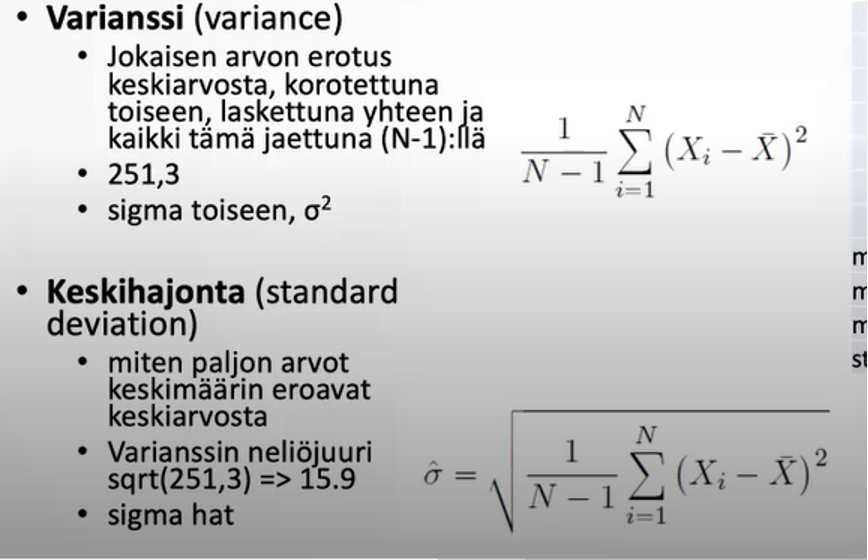
\includegraphics[keepaspectratio]{images/clipboard-209777777.png}}

Varianssi on siis keskihajonta korotettuna toiseen. Salmela (2026)

\part{R-komentoja}

Tänne kerään kurssin mittaan kootusti R-komentoja, funktioita,
koodinpätkiä eri aiheisiin liittyen.

\chapter{Kuvaajien piirtäminen}\label{kuvaajien-piirtuxe4minen}

\section{Histogrammi}\label{histogrammi}

Histogrammi piirretään \textbf{hist()} funktiolla

\begin{Shaded}
\begin{Highlighting}[]
\FunctionTok{hist}\NormalTok{(x , }\AttributeTok{breaks =} \DecValTok{30}\NormalTok{,  }\AttributeTok{xlim=}\FunctionTok{c}\NormalTok{(}\SpecialCharTok{{-}}\DecValTok{20}\NormalTok{,}\DecValTok{60}\NormalTok{))}
\end{Highlighting}
\end{Shaded}

\begin{itemize}
\item
  x ---\textgreater{} data, josta histogrammi piirretään
\item
  breaks = ---\textgreater{} voidaan määrittää millä välein palkkeja
  piirretään
\item
  xlim=c(alkupiste,loppupiste) ---\textgreater{} voidaan määritellä mikä
  osa x-akselista näkyy
\end{itemize}

Komennolla: \textbf{abline()} voidaan piirtää viivoja histogramiin

\begin{Shaded}
\begin{Highlighting}[]
\CommentTok{\#luodaan aineisto}
\NormalTok{x\_akseli }\OtherTok{\textless{}{-}} \FunctionTok{rnorm}\NormalTok{(}\DecValTok{100}\NormalTok{, }\DecValTok{10}\NormalTok{)}

\CommentTok{\# piirretään histogrammi ja kaksi viivaa }
\FunctionTok{hist}\NormalTok{(x\_akseli, }\AttributeTok{breaks =} \DecValTok{25}\NormalTok{, }\AttributeTok{xlim=}\FunctionTok{c}\NormalTok{(}\DecValTok{0}\NormalTok{,}\DecValTok{15}\NormalTok{)) }\CommentTok{\# }
\FunctionTok{abline}\NormalTok{(}\AttributeTok{v=} \DecValTok{10}\NormalTok{, }\AttributeTok{col=}\StringTok{"green"}\NormalTok{)}
\FunctionTok{abline}\NormalTok{(}\DecValTok{0}\NormalTok{,}\FloatTok{0.5}\NormalTok{, }\AttributeTok{col=}\StringTok{"red"}\NormalTok{)}
\end{Highlighting}
\end{Shaded}

\pandocbounded{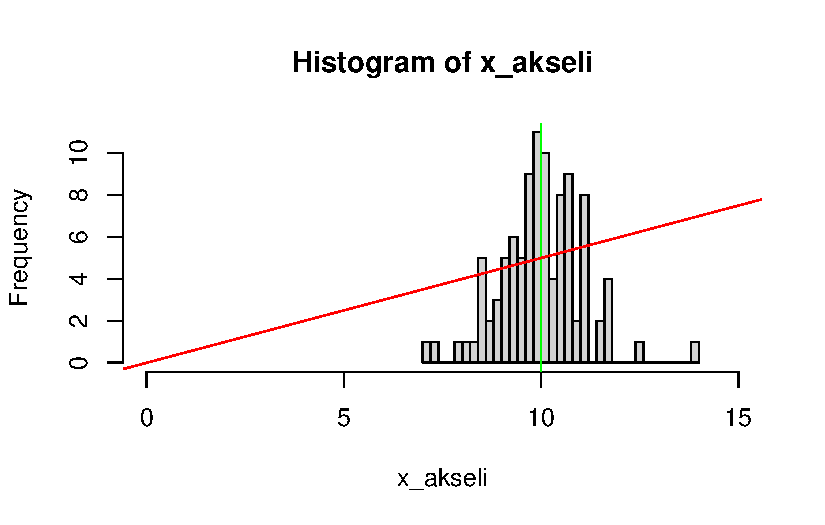
\includegraphics[keepaspectratio]{R_komentoja/KuvaajienPiirto_files/figure-pdf/unnamed-chunk-2-1.pdf}}

\begin{itemize}
\item
  \textbf{abline(a,b)} funktiossa

  \begin{itemize}
  \item
    a = vakio eli y-akselin leikkauskohta \# ( eli y:n arvo, kun x = 0),
  \item
    b = kulmakerroin
  \item
    pystysuoran viivan voi piirtää abline(v=a) komennolla, v = vertical
    tässä kontekstissa
  \item
    vaakasuoran puolestaan abline(h=a)
  \end{itemize}
\end{itemize}

\section{Pylväsdiagrammi}\label{pylvuxe4sdiagrammi}

\begin{Shaded}
\begin{Highlighting}[]
\NormalTok{heights\_var }\OtherTok{\textless{}{-}} \FunctionTok{c}\NormalTok{(}\AttributeTok{a=}\DecValTok{150}\NormalTok{,}\AttributeTok{b=} \DecValTok{160}\NormalTok{,}\AttributeTok{c=} \DecValTok{170}\NormalTok{,}\AttributeTok{d=} \DecValTok{180}\NormalTok{,}\AttributeTok{e=} \DecValTok{190}\NormalTok{)}
\FunctionTok{barplot}\NormalTok{(heights\_var)}
\end{Highlighting}
\end{Shaded}

\pandocbounded{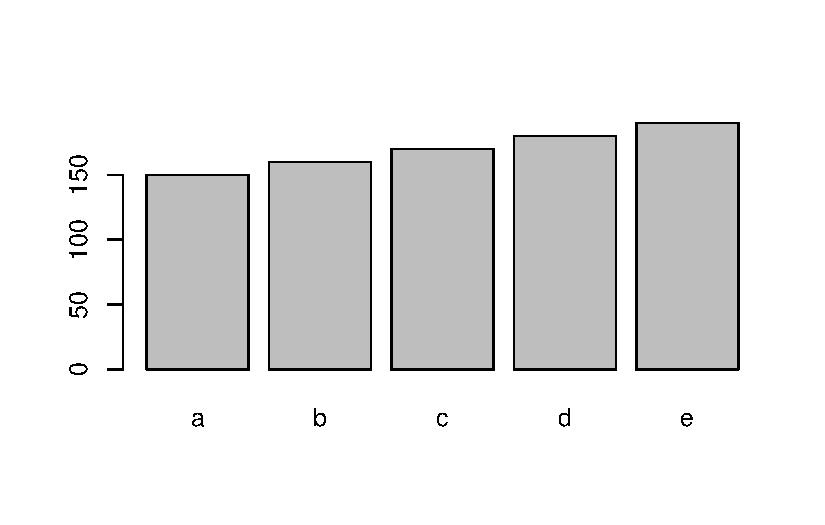
\includegraphics[keepaspectratio]{R_komentoja/KuvaajienPiirto_files/figure-pdf/unnamed-chunk-3-1.pdf}}

\section{Plot}\label{plot}

\begin{Shaded}
\begin{Highlighting}[]
\NormalTok{x }\OtherTok{\textless{}{-}} \FunctionTok{sample}\NormalTok{(}\DecValTok{100}\NormalTok{)}
\FunctionTok{plot}\NormalTok{(x)}
\end{Highlighting}
\end{Shaded}

\pandocbounded{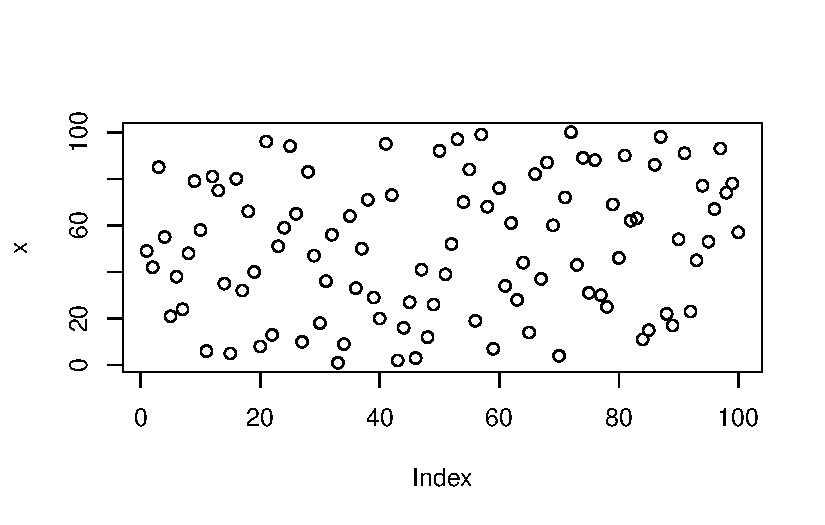
\includegraphics[keepaspectratio]{R_komentoja/KuvaajienPiirto_files/figure-pdf/unnamed-chunk-4-1.pdf}}

\chapter{ggplot paketti}\label{ggplot-paketti}

\section{Pylväsdiagrammi
ggplotilla}\label{pylvuxe4sdiagrammi-ggplotilla}

\begin{Shaded}
\begin{Highlighting}[]
\FunctionTok{library}\NormalTok{(ggplot2)}
\NormalTok{R1 }\OtherTok{\textless{}{-}} \FunctionTok{rnorm}\NormalTok{(}\DecValTok{1000}\NormalTok{,}\DecValTok{1}\NormalTok{)}
\NormalTok{R2 }\OtherTok{\textless{}{-}} \FunctionTok{rnorm}\NormalTok{(}\DecValTok{1000}\NormalTok{,}\DecValTok{3}\NormalTok{)}

\NormalTok{data }\OtherTok{\textless{}{-}} \FunctionTok{data.frame}\NormalTok{(}\AttributeTok{arvo =} \FunctionTok{c}\NormalTok{(R1,R2), ryhmä }\OtherTok{=} \FunctionTok{rep}\NormalTok{(}\FunctionTok{c}\NormalTok{(}\DecValTok{1}\NormalTok{,}\DecValTok{2}\NormalTok{), }\AttributeTok{each=}\DecValTok{1000}\NormalTok{))}

\FunctionTok{ggplot}\NormalTok{(data, }\FunctionTok{aes}\NormalTok{(}\AttributeTok{x =} \FunctionTok{as.factor}\NormalTok{(ryhmä), }\AttributeTok{y =}\NormalTok{ arvo, }\AttributeTok{fill =}\NormalTok{ ryhmä)) }\SpecialCharTok{+}
  \CommentTok{\# Piirretään keskiarvopylväät}
  \FunctionTok{stat\_summary}\NormalTok{(}\AttributeTok{fun =} \StringTok{"mean"}\NormalTok{, }\AttributeTok{geom =} \StringTok{"bar"}\NormalTok{, }\AttributeTok{color =} \StringTok{"black"}\NormalTok{, }\AttributeTok{width =} \FloatTok{0.5}\NormalTok{, }\AttributeTok{na.rm =} \ConstantTok{TRUE}\NormalTok{) }\SpecialCharTok{+}
  \CommentTok{\# Lisätään virhejanat (Standard Error)}
  \FunctionTok{stat\_summary}\NormalTok{(}\AttributeTok{fun.data =} \StringTok{"mean\_se"}\NormalTok{, }\AttributeTok{geom =} \StringTok{"errorbar"}\NormalTok{,}\AttributeTok{color =} \StringTok{"red"}\NormalTok{,  }\AttributeTok{width =} \FloatTok{0.3}\NormalTok{,}\AttributeTok{na.rm =} \ConstantTok{TRUE}\NormalTok{) }\SpecialCharTok{+}
  
  \FunctionTok{labs}\NormalTok{(}\AttributeTok{title =} \StringTok{"Mittaustulokset ryhmittäin"}\NormalTok{,}
       \AttributeTok{x =} \StringTok{"Ryhmä"}\NormalTok{,}
       \AttributeTok{y =} \StringTok{"Keskiarvotulos"}\NormalTok{) }\SpecialCharTok{+}
    \FunctionTok{theme\_minimal}\NormalTok{()}
\end{Highlighting}
\end{Shaded}

\pandocbounded{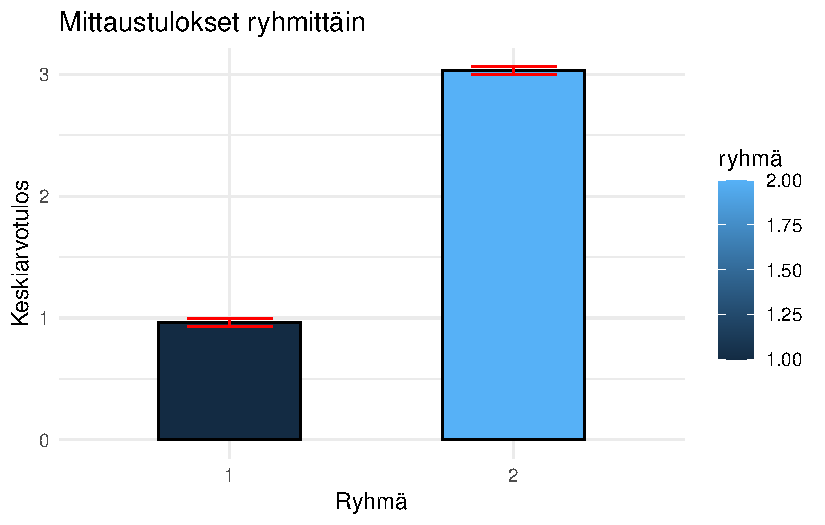
\includegraphics[keepaspectratio]{R_komentoja/ggplot_files/figure-pdf/unnamed-chunk-1-1.pdf}}

\begin{itemize}
\item
  ggplot(data, aes(x = ryhmä, y = arvo, fill = ryhmä))

  \begin{itemize}
  \item
    data --\textgreater{} datasetti
  \item
    aes(x = sarake, joka tulee x-akselille, y = sarake, joka tulee
    y-akselille, fill = muuttaa väriä arvoa sarakkeen alkiosta toiseen)

    \begin{itemize}
    \tightlist
    \item
      as.factor(ryhmä) --\textgreater{} kun merkataan as.factor saadaan
      tulostettua vain luvut 1 ja 2. Eli ei tule desimaaleja niiden
      väliin
    \end{itemize}
  \end{itemize}
\item
  stat\_summary(fun = ``mean'', geom = ``bar'', color = ``black'', width
  = 0.9, na.rm = TRUE)

  \begin{itemize}
  \item
    fun = käytettävä funktio
  \item
    geom = mikä muoto piirretään
  \item
    color = väri
  \item
    width = palkin leveys
  \item
    na.rm = poistetaan puuttuvat arvot
  \end{itemize}
\item
  stat\_summary(fun.data = ``mean\_se'', geom = ``errorbar'',color =
  ``red'', width = 0.3,na.rm = TRUE)

  \begin{itemize}
  \tightlist
  \item
    luottamusvälien / virhepalkkien piirto
  \end{itemize}
\item
  labs() --\textgreater{} otsikot
\item
  theme\_minimal() --\textgreater{} teema
\end{itemize}

\chapter{Datasetin luominen}\label{datasetin-luominen}

\section{Datan avaaminen}\label{datan-avaaminen}

\begin{Shaded}
\begin{Highlighting}[]
\FunctionTok{library}\NormalTok{(readr)}

\NormalTok{PerceptualLearnData }\OtherTok{\textless{}{-}} \FunctionTok{read\_csv}\NormalTok{(}\StringTok{"data/PerceptualLearn/PerceptualLearnData.csv"}\NormalTok{)}

\FunctionTok{View}\NormalTok{(PerceptualLearnData)}
\end{Highlighting}
\end{Shaded}

\begin{itemize}
\item
  readr paketista saa csv tiedostojen lukemisen komennot
\item
  read\_csv()

  \begin{itemize}
  \item
    hakee tiedoston
  \item
    tiedoston täytyy olla projektikansiossa ja mikäli se sijaitsee
    projektikansion alakansiossa täytyy kirjoittaa koko polku
    projektikansiosta eteenpäin

    \begin{itemize}
    \item
      Esim. Projektikansiossa alakansio data ja sen alakansio
      PerceptualLearn, jossa tiedosto sijaitsee
    \item
      kirjoitetaan ``data/PerceptualLearn/PerceptualLearnData.csv''
    \end{itemize}
  \end{itemize}
\item
  View()

  \begin{itemize}
  \tightlist
  \item
    näyttää haetun ja muuttujaan talletetun tiedoston
  \end{itemize}
\end{itemize}

\section{Datasetin kuvailu}\label{datasetin-kuvailu}

aggregate() funktiolla

\begin{Shaded}
\begin{Highlighting}[]
\FunctionTok{aggregate}\NormalTok{(Confidence }\SpecialCharTok{\textasciitilde{}}\NormalTok{ Session, }\AttributeTok{data =}\NormalTok{ PerceptualLearnData, }\AttributeTok{FUN =}\NormalTok{ mean)}
\end{Highlighting}
\end{Shaded}

\begin{itemize}
\item
  Voidaan laskea annettusta datasetistä asioita halutulla funktioilla
  ryhmitellen
\item
  data = \textless- datasetti, josta tiedot haetaan

  \begin{itemize}
  \tightlist
  \item
    datasetistä PerceptualLearnData löytyy sarakkeet Confidence ja
    Session
  \end{itemize}
\item
  ``Confidence'' paikalle sarake, jossa on haluttu tieto
\item
  ``Session'' paikalle ryhmittelevä muuttuja eli sarake, jonka mukaan
  tiedot jaetaan ryhmiin

  \begin{itemize}
  \item
    Esimerkissiä oli 3 eri sessiota, jossa mitattiin itseluottamusta
  \item
    Tuloksena tulee siis 3:n eri session itseluottamusten keskiarvot
    eriteltynä
  \end{itemize}
\item
  FUN = \textless- funktio, jotka käytetään. Esimerkissä mean() eli
  keskiarvo
\end{itemize}

Havainnollistava esimerkki

\begin{Shaded}
\begin{Highlighting}[]
\NormalTok{R1 }\OtherTok{\textless{}{-}} \FunctionTok{rnorm}\NormalTok{(}\DecValTok{1000}\NormalTok{,}\DecValTok{1}\NormalTok{)}
\NormalTok{R2 }\OtherTok{\textless{}{-}} \FunctionTok{rnorm}\NormalTok{(}\DecValTok{1000}\NormalTok{,}\DecValTok{3}\NormalTok{)}

\NormalTok{data }\OtherTok{\textless{}{-}} \FunctionTok{data.frame}\NormalTok{(}\AttributeTok{arvo =} \FunctionTok{c}\NormalTok{(R1,R2), ryhmä }\OtherTok{=} \FunctionTok{rep}\NormalTok{(}\FunctionTok{c}\NormalTok{(}\DecValTok{1}\NormalTok{,}\DecValTok{2}\NormalTok{), }\AttributeTok{each=}\DecValTok{1000}\NormalTok{))}

\FunctionTok{aggregate}\NormalTok{(arvo }\SpecialCharTok{\textasciitilde{}}\NormalTok{ ryhmä, }\AttributeTok{data =}\NormalTok{ data, }\AttributeTok{FUN =}\NormalTok{ mean)}
\end{Highlighting}
\end{Shaded}

\begin{verbatim}
  ryhmä     arvo
1     1 1.007348
2     2 3.025210
\end{verbatim}

\begin{itemize}
\item
  Tässä havainnollistuksen vuoksi laskettiin aggregate funktiolla
  keskiarvot ryhmille 1 ja 2.
\item
  R1 keskiarvoksi määritettiin rnorm() funktiolla 1 ja R2 funktiolle 3
\item
  aggregate() funktiolla saatiin laskettua ryhmitellyt keskiarvot
\end{itemize}

summary() funktiolla

\begin{Shaded}
\begin{Highlighting}[]
\FunctionTok{summary}\NormalTok{(PerceptualLearnData}\SpecialCharTok{$}\NormalTok{Confidence)}
\end{Highlighting}
\end{Shaded}

\begin{itemize}
\item
  antaa datasetin minimin, 1. kvartiilin mediaanin, keskiarvon, 3.
  kvartiilin ja maksimin sarakkeittain
\item
  voi valita myös vain yhden sarakkeen viittaamalla \$ merkillä
\end{itemize}

names() funktiolla

\begin{Shaded}
\begin{Highlighting}[]
\NormalTok{R1 }\OtherTok{\textless{}{-}} \FunctionTok{rnorm}\NormalTok{(}\DecValTok{5}\NormalTok{,}\DecValTok{0}\NormalTok{)}
\NormalTok{R2 }\OtherTok{\textless{}{-}} \FunctionTok{rnorm}\NormalTok{(}\DecValTok{5}\NormalTok{,}\DecValTok{1}\NormalTok{)}

\NormalTok{data }\OtherTok{\textless{}{-}} \FunctionTok{data.frame}\NormalTok{(}\AttributeTok{arvo =} \FunctionTok{c}\NormalTok{(R1,R2), ryhmä }\OtherTok{=} \FunctionTok{rep}\NormalTok{(}\FunctionTok{c}\NormalTok{(}\DecValTok{1}\NormalTok{,}\DecValTok{2}\NormalTok{), }\AttributeTok{each=}\DecValTok{5}\NormalTok{))}

\FunctionTok{names}\NormalTok{(data)}
\end{Highlighting}
\end{Shaded}

\begin{verbatim}
[1] "arvo"  "ryhmä"
\end{verbatim}

\begin{itemize}
\tightlist
\item
  palauttaa datasetin sarakkeiden nimet
\end{itemize}

\section{rnorm()}\label{rnorm}

\begin{Shaded}
\begin{Highlighting}[]
\FunctionTok{rnorm}\NormalTok{(n, mean, sd) }
\end{Highlighting}
\end{Shaded}

\begin{itemize}
\item
  luo normaalijakaumaa noudattavan vektorin, jossa

  \begin{itemize}
  \item
    n ---\textgreater{} lukumäärä
  \item
    mean ---\textgreater{} keskiarvo (oletuksena 0)
  \item
    sd ---\textgreater{} keskihajonta (oletuksena 1)
  \end{itemize}
\item
  Esim. alla luodaan normaalijakaumaa noudattava 10 alkion vektori,
  jonka keskiarvo on 6 ja keskihajonta 2.
\end{itemize}

\begin{Shaded}
\begin{Highlighting}[]
\FunctionTok{rnorm}\NormalTok{(}\DecValTok{10}\NormalTok{, }\DecValTok{6}\NormalTok{, }\DecValTok{2}\NormalTok{) }
\end{Highlighting}
\end{Shaded}

\begin{verbatim}
 [1]  4.014193  4.754470  8.909081  3.646791 12.851807 11.051411  3.664269
 [8]  4.762090  3.513346  7.818483
\end{verbatim}

Tarkistetaan, että keskiarvo ja keskihajonta pitävät paikkansa.

\begin{Shaded}
\begin{Highlighting}[]
\NormalTok{vekt10 }\OtherTok{\textless{}{-}} \FunctionTok{rnorm}\NormalTok{(}\DecValTok{10}\NormalTok{,}\DecValTok{6}\NormalTok{,}\DecValTok{2}\NormalTok{) }
\NormalTok{vekt100 }\OtherTok{\textless{}{-}} \FunctionTok{rnorm}\NormalTok{(}\DecValTok{100}\NormalTok{,}\DecValTok{6}\NormalTok{,}\DecValTok{2}\NormalTok{) }
\NormalTok{vekt1000 }\OtherTok{\textless{}{-}} \FunctionTok{rnorm}\NormalTok{(}\DecValTok{1000}\NormalTok{,}\DecValTok{6}\NormalTok{,}\DecValTok{2}\NormalTok{) }

\NormalTok{m1 }\OtherTok{\textless{}{-}} \FunctionTok{mean}\NormalTok{(vekt10) }
\NormalTok{sd1 }\OtherTok{\textless{}{-}} \FunctionTok{sd}\NormalTok{(vekt10) }
\NormalTok{m2 }\OtherTok{\textless{}{-}} \FunctionTok{mean}\NormalTok{(vekt100) }
\NormalTok{sd2 }\OtherTok{\textless{}{-}} \FunctionTok{sd}\NormalTok{(vekt100) }
\NormalTok{m3 }\OtherTok{\textless{}{-}} \FunctionTok{mean}\NormalTok{(vekt1000) }
\NormalTok{sd3 }\OtherTok{\textless{}{-}} \FunctionTok{sd}\NormalTok{(vekt1000) }
\NormalTok{RivNimet }\OtherTok{\textless{}{-}} \FunctionTok{c}\NormalTok{(}\StringTok{"Keskiarvo"}\NormalTok{, }\StringTok{"Keskihajonta"}\NormalTok{)}

\FunctionTok{data.frame}\NormalTok{(}\AttributeTok{N10 =} \FunctionTok{c}\NormalTok{(m1,sd1), }\AttributeTok{N100 =} \FunctionTok{c}\NormalTok{(m2,sd2), }\AttributeTok{N1000 =} \FunctionTok{c}\NormalTok{(m3, sd3), }\AttributeTok{row.names =}\NormalTok{ RivNimet)}
\end{Highlighting}
\end{Shaded}

\begin{verbatim}
                  N10     N100    N1000
Keskiarvo    6.098229 6.103335 5.986777
Keskihajonta 2.348996 1.946751 1.964323
\end{verbatim}

Isommalla n:llä näyttäisi osuvan vielä tarkemmin kohdalleen.

\section{set.seed() funktio}\label{set.seed-funktio}

\begin{Shaded}
\begin{Highlighting}[]
\FunctionTok{set.seed}\NormalTok{(}\DecValTok{123}\NormalTok{)}
\end{Highlighting}
\end{Shaded}

\begin{itemize}
\item
  Määrittää mitä satunnaislukuja käytetään
\item
  laitetaan (yleensä) vain kerran skriptin alkuun
\item
  Hyöty on se, että määrittää joka kerta samat satunnaisluvut eli jos
  ajaa saman skriptin kaksi kertaa molemmilla kerroilla laskelmiin tulee
  samat luvut ja kuvaajat näyttävät samanlaisilta
\end{itemize}

\subsection{Havainnollistava
esimerkki}\label{havainnollistava-esimerkki}

\begin{Shaded}
\begin{Highlighting}[]
\FunctionTok{set.seed}\NormalTok{(}\DecValTok{123}\NormalTok{) }

\NormalTok{Alkupiste }\OtherTok{\textless{}{-}} \FunctionTok{rnorm}\NormalTok{(}\DecValTok{1}\NormalTok{)}
\NormalTok{Jatkopiste }\OtherTok{\textless{}{-}} \FunctionTok{rnorm}\NormalTok{(}\DecValTok{1}\NormalTok{) }

\FunctionTok{data.frame}\NormalTok{(}\StringTok{"Alku"} \OtherTok{=}\NormalTok{ Alkupiste, }\StringTok{"Jatkopiste"} \OtherTok{=}\NormalTok{ Jatkopiste)}
\end{Highlighting}
\end{Shaded}

\begin{verbatim}
        Alku Jatkopiste
1 -0.5604756 -0.2301775
\end{verbatim}

\begin{itemize}
\item
  Ensimmäinen luotu satunnaisluku eli Alkupiste on set.seed(123) listan
  ensimmäinen luku
\item
  Toinen luotu satunnaisluku eli Jatkopiste on set.seed(123) listan
  toinen luku
\end{itemize}

\begin{Shaded}
\begin{Highlighting}[]
\FunctionTok{set.seed}\NormalTok{(}\DecValTok{123}\NormalTok{)}
\NormalTok{alkupiste }\OtherTok{\textless{}{-}} \FunctionTok{rnorm}\NormalTok{(}\DecValTok{1}\NormalTok{)}

\FunctionTok{set.seed}\NormalTok{(}\DecValTok{123}\NormalTok{)}
\NormalTok{uusialkupiste }\OtherTok{\textless{}{-}} \FunctionTok{rnorm}\NormalTok{(}\DecValTok{1}\NormalTok{)}

\FunctionTok{data.frame}\NormalTok{(}\StringTok{"Alku"} \OtherTok{=}\NormalTok{ alkupiste, }\StringTok{"UusiAlku"} \OtherTok{=}\NormalTok{ uusialkupiste)}
\end{Highlighting}
\end{Shaded}

\begin{verbatim}
        Alku   UusiAlku
1 -0.5604756 -0.5604756
\end{verbatim}

\begin{itemize}
\item
  Ensimmäinen satunnaisluku set.seed(123) listan ensimmäinen luku
\item
  Koska set.seed(123) laitettiin skriptiin uudelleen se nollaa listan ja
  sitä lähdetään käymään uudelleen läpi

  \begin{itemize}
  \tightlist
  \item
    Siksi toinen luotu satunnaisluku eli UusiAlku on sama
  \end{itemize}
\end{itemize}

\subsubsection{Ero rnorm() funktiossa set.seed() kanssa ja
ilman}\label{ero-rnorm-funktiossa-set.seed-kanssa-ja-ilman}

Set.seedin() kanssa rnorm() luo siis satunnaisluvut tietystä listasta ja
ne toistuvat jokaisella ajokerralla samalla tavalla. Ilman set.seed()
funktiota jokaisella ajokerralla rnorm() luo eri satunnaisluvut.

Set.seedin kanssa

\begin{Shaded}
\begin{Highlighting}[]
\NormalTok{set.seed(123)}
\NormalTok{AinaSamat \textless{}{-} numeric(10) }
\NormalTok{for( i in 1:10)\{}
\NormalTok{AinaSamat[i] \textless{}{-} rnorm(1)}
\NormalTok{\}}
\NormalTok{AinaSamat}
\end{Highlighting}
\end{Shaded}

Ilman set.seedia

\begin{Shaded}
\begin{Highlighting}[]

\NormalTok{AinaErit \textless{}{-} numeric(10)}
\NormalTok{for( i in 1:10)\{}
\NormalTok{  AinaErit[i] \textless{}{-} rnorm(1)}
\NormalTok{\}}
\NormalTok{AinaErit}
\end{Highlighting}
\end{Shaded}

Yllä voi kokeilla ajaa koodinpätkät niiin monta kertaa kuin haluaa.
Set.seedin kanssa jokaisella ajokerralla tulee samat luvut, kun ilman
sitä joka kerta tulee eri luvut.

\section{Data framen luominen}\label{data-framen-luominen}

\begin{Shaded}
\begin{Highlighting}[]
\NormalTok{R1 }\OtherTok{\textless{}{-}} \FunctionTok{rnorm}\NormalTok{(}\DecValTok{5}\NormalTok{,}\DecValTok{0}\NormalTok{)}
\NormalTok{R2 }\OtherTok{\textless{}{-}} \FunctionTok{rnorm}\NormalTok{(}\DecValTok{5}\NormalTok{,}\DecValTok{1}\NormalTok{)}

\NormalTok{data }\OtherTok{\textless{}{-}} \FunctionTok{data.frame}\NormalTok{(}\AttributeTok{arvo =} \FunctionTok{c}\NormalTok{(R1,R2), ryhmä }\OtherTok{=} \FunctionTok{rep}\NormalTok{(}\FunctionTok{c}\NormalTok{(}\DecValTok{1}\NormalTok{,}\DecValTok{2}\NormalTok{), }\AttributeTok{each=}\DecValTok{5}\NormalTok{))}
\NormalTok{data}
\end{Highlighting}
\end{Shaded}

\begin{verbatim}
          arvo ryhmä
1  -0.23017749     1
2   1.55870831     1
3   0.07050839     1
4   0.12928774     1
5   1.71506499     1
6   1.46091621     2
7  -0.26506123     2
8   0.31314715     2
9   0.55433803     2
10  2.22408180     2
\end{verbatim}

data.frame(sarake1, sarake2, sarake3, \ldots)

\begin{itemize}
\item
  Eli sulkuihin erotellaan pilkuilla eri sarakkeisiin menevä data
\item
  sarakkeet pystyy nimeämään laittamalla arvojen eteen nimen ja = (esim.
  arvo=R1)
\item
  esimerkissä käytetty c() eli combine funktiota, joka yhdistää kahdesta
  vektorista yhden

  \begin{itemize}
  \tightlist
  \item
    c() funktiolla saa siis yhdistettyä useamman vektorin yhden
    sarakkeen alle
  \end{itemize}
\item
  row.names= argumentilla saa rivit nimettyä

  \begin{itemize}
  \item
    täytyy viitata vektoriin esim. ylemmässä keskiarvo ja keskihajonta
    tehtävässä luotiin kirjainvektori RivNimet, johon sitten viitattiin

    \begin{itemize}
    \tightlist
    \item
      RivNimet \textless- c(``Keskiarvo'' , ``Keskihajonta'')
    \end{itemize}
  \end{itemize}
\end{itemize}

\section{Satunnaistaminen tai satunnaisnumero sample()
funktiolla}\label{satunnaistaminen-tai-satunnaisnumero-sample-funktiolla}

\begin{Shaded}
\begin{Highlighting}[]
\FunctionTok{sample}\NormalTok{(x, size, }\AttributeTok{replace =} \ConstantTok{FALSE}\NormalTok{, }\AttributeTok{prob =} \ConstantTok{NULL}\NormalTok{) }
\end{Highlighting}
\end{Shaded}

\begin{itemize}
\item
  x -\textgreater{} datajoukko, josta numerot vedetään

  \begin{itemize}
  \item
    esim. 1:10, generoi numeroita väliltä 1-10
  \item
    voi myös viitata muuttujaan
  \end{itemize}
\item
  size -\textgreater{} montako numeroa otetaan

  \begin{itemize}
  \tightlist
  \item
    esim 1 palauttaa yhden lukuarvon ja 2 2 lukuarvoa jne
  \end{itemize}
\item
  replace = FALSE -\textgreater{} palautetaanko jo nostetut arvot
  koriin, jolloin niitä voidaan käyttää uudelleen vai käytetäänko
  jokaista arvoa maksimissaan kerran

  \begin{itemize}
  \item
    oletuksena FALSE eli arvoja käytetään vain kerran

    \begin{itemize}
    \tightlist
    \item
      esim. permutaatiotestissä joka arvoa käyteetään vain kerran
    \end{itemize}
  \item
    jos vaihtaa TRUE niin arvoja voidaan käyttää useampaan otteeseen

    \begin{itemize}
    \tightlist
    \item
      bootstrap menetelmässä arvoja puolestaan käytetään useampaan
      otteeseseen
    \end{itemize}
  \end{itemize}
\end{itemize}

\section{Uuden kansion luominen
dir.create()}\label{uuden-kansion-luominen-dir.create}

\begin{Shaded}
\begin{Highlighting}[]
\FunctionTok{dir.create}\NormalTok{(}\StringTok{"uusi\_kansio"}\NormalTok{) }
\end{Highlighting}
\end{Shaded}

\begin{itemize}
\item
  Luo uuden kansion työskentelykansioon

  \begin{itemize}
  \tightlist
  \item
    työskentelykansion voi aina tarkistaa getwd() funktiolla
  \end{itemize}
\end{itemize}

\begin{Shaded}
\begin{Highlighting}[]
\FunctionTok{dir.create}\NormalTok{(}\StringTok{"kurssi/viikko1"}\NormalTok{, }\AttributeTok{recursive =} \ConstantTok{TRUE}\NormalTok{)}
\end{Highlighting}
\end{Shaded}

\begin{itemize}
\item
  recursive = TRUE -\textgreater{} mahdollistaa yhdellä kerralla kansion
  ja alikansion luomisen

  \begin{itemize}
  \tightlist
  \item
    esimerkissä luo kansion kurssi ja siihen alikansion viikko1 kansion
  \end{itemize}
\end{itemize}

Hyvä muistaa

\begin{itemize}
\item
  Ei ylikirjoita olemassaolevien kansioiden päälle, vaan antaa
  varoituksen
\item
  varmista, että nojaviivat ovat eteenpäin, jos ei toimi

  \begin{itemize}
  \tightlist
  \item
    vain yksi kenoviiva kansioiden välille
  \end{itemize}
\end{itemize}

\section{Kansion luominen if-lauseen
kanssa}\label{kansion-luominen-if-lauseen-kanssa}

\begin{Shaded}
\begin{Highlighting}[]
\CommentTok{\#| eval: false }
\NormalTok{uusi\_paakansio }\OtherTok{\textless{}{-}} \StringTok{"Koulutehtava"}

\ControlFlowTok{if}\NormalTok{ (}\SpecialCharTok{!}\FunctionTok{dir.exists}\NormalTok{(uusi\_paakansio)) \{}
  \FunctionTok{dir.create}\NormalTok{(uusi\_paakansio)}
\NormalTok{\}}
\end{Highlighting}
\end{Shaded}

\begin{itemize}
\item
  Kansio voi olla järkevää luoda if lausekkeen kanssa koska

  \begin{itemize}
  \item
    se yrittää luoda kansion, vain jos sen nimistä kansiota ei vielä ole
    olemassa
  \item
    Eli sen jälkeen, kun kansio on jo luotu, niin seuraavilla
    ajokerroilla ei yritetä turhaan luoda sitä uudestaan

    \begin{itemize}
    \tightlist
    \item
      olemassa olevalle kansiolle ei käy mitään uusilla ajokerroilla,
      vaikka sitä pyrittäisiin luomaan uudestaan, mutta se antaa
      virheilmoituksen/varoituksen konsoliin, joka tekee siitä
      sekavamman
    \end{itemize}
  \end{itemize}
\item
  ! \textless- merkki tarkoittaa loogista ei operaattoria

  \begin{itemize}
  \item
    eli if lauseen ehto menee: jos uusi\_paakansio nimistä kansiota ei
    ole olemassa niin tee seuraava asia

    \begin{itemize}
    \tightlist
    \item
      luo uusi kansio dir.create() funktiolla
    \end{itemize}
  \item
    ilman ! merkkiä ehto menisi siis: jos uusi\_paakansio on olemassa
    niin tee seuraava asia
  \end{itemize}
\end{itemize}

\section{Tiedosto ja kansiopolun muuttaminen
file.rename()}\label{tiedosto-ja-kansiopolun-muuttaminen-file.rename}

\begin{Shaded}
\begin{Highlighting}[]
\FunctionTok{file.rename}\NormalTok{(from, to) }
\end{Highlighting}
\end{Shaded}

\begin{itemize}
\item
  file.rename() funktiossa

  \begin{itemize}
  \item
    from kohtaan alkuperäinen siirrettävän kansion nimi
  \item
    to kohtaan uuden yläkansion nimi / siirrettävän kansion nimi
  \end{itemize}
\end{itemize}

\begin{Shaded}
\begin{Highlighting}[]
\FunctionTok{dir.create}\NormalTok{(}\StringTok{"kurssi/viikko1"}\NormalTok{, }\AttributeTok{recursive =} \ConstantTok{TRUE}\NormalTok{)}
\FunctionTok{dir.create}\NormalTok{(}\StringTok{"Salatut\_elamat"}\NormalTok{)}

\FunctionTok{file.rename}\NormalTok{(}\StringTok{"kurssi"}\NormalTok{,}\StringTok{"Salatut\_elamat/kurssi"}\NormalTok{)}
\end{Highlighting}
\end{Shaded}

Esim.

\begin{itemize}
\item
  Luotiin kansio kurssi ja sen alakansio viikko1
\item
  Lisäksi luotiin kansio Salatut\_elamat
\item
  file.rename() funktiolla saadaan siirrettyä kurssi kansio
  Salatut\_elamat kansion alle

  \begin{itemize}
  \tightlist
  \item
    koko ``kurssi'' kansio siirtyy eli sen alla oleva viikko1 siirtyy
    samalla
  \end{itemize}
\end{itemize}

\section{Tiedostopolun kirjoittaminen file.path()
funktiolla}\label{tiedostopolun-kirjoittaminen-file.path-funktiolla}

\begin{Shaded}
\begin{Highlighting}[]
\FunctionTok{file.path}\NormalTok{(}\StringTok{"tietokone"}\NormalTok{, }\StringTok{"käyttäjä"}\NormalTok{, }\StringTok{"omatkansiot"}\NormalTok{, }\StringTok{"data"}\NormalTok{, }\StringTok{"measures"}\NormalTok{)}
\end{Highlighting}
\end{Shaded}

Kun kirjoittaa file.path() funktioon esimerkin mukaisesti R rakentaa sen
näin:

\begin{enumerate}
\def\labelenumi{\arabic{enumi}.}
\item
  Ottaa sanan tietokone
\item
  Lisää erottimen /
\item
  Ottaa sanan käyttäjä
\item
  Lisää erottimen / jne.
\end{enumerate}

\begin{itemize}
\tightlist
\item
  Eli file.path() funktiolla saa tiedostopolun helposti talteen ilman
  virheitä ja kenoviivojen kanssa sähläämistä
\end{itemize}

\section{Tiedostojen hakeminen ylä- tai
alakansioista}\label{tiedostojen-hakeminen-yluxe4--tai-alakansioista}

..

\begin{itemize}
\tightlist
\item
  kaksi pistettä tiedostonimessä tarkoittaa, että siirrytään yksi
  kansiotaso ylöspäin
\end{itemize}

\begin{Shaded}
\begin{Highlighting}[]
\NormalTok{data }\OtherTok{\textless{}{-}} \FunctionTok{read\_csv}\NormalTok{(}\StringTok{"../data/PerceptualLearnData.csv"}\NormalTok{)}
\end{Highlighting}
\end{Shaded}

\begin{itemize}
\tightlist
\item
  esimerkissä skripti on pääkansion alakansiossa ja haluttiin siirtyä
  yläkansioon ja sieltä toiseen alakansioon nimeltä data, jossa
  PerceptualLearnData.csv sijaitsee.
\end{itemize}

\chapter{Tilastotestejä}\label{tilastotestejuxe4}

\section{T-testi}\label{t-testi}

Testaa onko kahden ryhmän keskiarvojen välinen ero tilastollisesti
merkitsevä.

\subsection{T-testi syöttämällä suoraan kaksi
ryhmää}\label{t-testi-syuxf6ttuxe4muxe4lluxe4-suoraan-kaksi-ryhmuxe4uxe4}

\begin{Shaded}
\begin{Highlighting}[]
\NormalTok{R1 }\OtherTok{\textless{}{-}} \FunctionTok{rnorm}\NormalTok{(}\DecValTok{50}\NormalTok{,}\DecValTok{0}\NormalTok{)}
\NormalTok{R2 }\OtherTok{\textless{}{-}} \FunctionTok{rnorm}\NormalTok{(}\DecValTok{50}\NormalTok{,}\DecValTok{1}\NormalTok{)}

\FunctionTok{t.test}\NormalTok{(R1, R2)}
\end{Highlighting}
\end{Shaded}

\begin{verbatim}

    Welch Two Sample t-test

data:  R1 and R2
t = -5.6416, df = 93.304, p-value = 1.795e-07
alternative hypothesis: true difference in means is not equal to 0
95 percent confidence interval:
 -1.4724214 -0.7057542
sample estimates:
 mean of x  mean of y 
-0.1095770  0.9795108 
\end{verbatim}

Mitä tietoja testi näyttää

\begin{itemize}
\item
  t-arvo: montako keskivirheen mittaa ryhmien keskiarvot eroavat
\item
  df = degrees of freedom = vapausasteet
\item
  p-value eli p-arvo
\item
  95 percent confidence interval = luottamusväli eli Väli, jolla ryhmien
  todellinen keskiarvojen erotus on 95 \% todennäköisyydellä.

  \begin{itemize}
  \tightlist
  \item
    eli 95 kertaa sadasta keskiarvojen erotus osuu välille ja 5 kertaa
    sadasta ulkopuolelle
  \end{itemize}
\item
  sample estimates: ryhmien omat keskiarvot
\end{itemize}

\subsection{T-testi kaavamuodossa (tällöin voidaan hakea tieto
dataframesta)}\label{t-testi-kaavamuodossa-tuxe4lluxf6in-voidaan-hakea-tieto-dataframesta}

\begin{Shaded}
\begin{Highlighting}[]
\NormalTok{R1 }\OtherTok{\textless{}{-}} \FunctionTok{rnorm}\NormalTok{(}\DecValTok{50}\NormalTok{,}\DecValTok{0}\NormalTok{)}
\NormalTok{R2 }\OtherTok{\textless{}{-}} \FunctionTok{rnorm}\NormalTok{(}\DecValTok{50}\NormalTok{,}\DecValTok{1}\NormalTok{)}

\NormalTok{data }\OtherTok{\textless{}{-}} \FunctionTok{data.frame}\NormalTok{(}\AttributeTok{arvo =} \FunctionTok{c}\NormalTok{(R1,R2), ryhmä }\OtherTok{=} \FunctionTok{rep}\NormalTok{(}\FunctionTok{c}\NormalTok{(}\DecValTok{1}\NormalTok{,}\DecValTok{2}\NormalTok{), }\AttributeTok{each=}\DecValTok{50}\NormalTok{)) }

\FunctionTok{t.test}\NormalTok{(arvo }\SpecialCharTok{\textasciitilde{}}\NormalTok{ ryhmä, }\AttributeTok{data =}\NormalTok{ data) }
\end{Highlighting}
\end{Shaded}

\begin{verbatim}

    Welch Two Sample t-test

data:  arvo by ryhmä
t = -5.0954, df = 96.369, p-value = 1.731e-06
alternative hypothesis: true difference in means between group 1 and group 2 is not equal to 0
95 percent confidence interval:
 -1.5095293 -0.6631704
sample estimates:
mean in group 1 mean in group 2 
     -0.2373269       0.8490229 
\end{verbatim}

\section{Korrelaatio}\label{korrelaatio}

\begin{Shaded}
\begin{Highlighting}[]
\NormalTok{x }\OtherTok{\textless{}{-}} \FunctionTok{c}\NormalTok{(}\DecValTok{1}\NormalTok{, }\DecValTok{2}\NormalTok{, }\DecValTok{3}\NormalTok{, }\DecValTok{4}\NormalTok{, }\DecValTok{5}\NormalTok{)}
\NormalTok{y }\OtherTok{\textless{}{-}} \FunctionTok{c}\NormalTok{(}\DecValTok{2}\NormalTok{, }\DecValTok{4}\NormalTok{, }\DecValTok{5}\NormalTok{, }\DecValTok{4}\NormalTok{, }\DecValTok{6}\NormalTok{)}

\FunctionTok{cor}\NormalTok{(x, y) }
\end{Highlighting}
\end{Shaded}

\begin{verbatim}
[1] 0.8528029
\end{verbatim}

cor(x,y)

\begin{itemize}
\item
  laskee x:n ja y:n korrelaation, jos ne ovat vektoreita

  \begin{itemize}
  \tightlist
  \item
    jos matriiseja niin laskee sarakkeiden x:n ja y:n sarakkeiden
    välisen korrelaation
  \end{itemize}
\item
  oletuksena pearsonin korrelaatio

  \begin{itemize}
  \item
    voi muuttaa spearmanin tai kendallin korrelaatioon argumentilla
    method =

    \begin{itemize}
    \tightlist
    \item
      method = ``spearman'', method = ``kendall'', method = ``pearson''
    \end{itemize}
  \end{itemize}
\item
  \texttt{use\ =\ "pairwise.complete"} NA arvot jätetään huomioimatta
  (Thulin (2024))
\end{itemize}

\chapter{Matemaattisia funktioita}\label{matemaattisia-funktioita}

\section{Kertoma: factorial()}\label{kertoma-factorial}

\begin{Shaded}
\begin{Highlighting}[]
\FunctionTok{factorial}\NormalTok{(}\DecValTok{3}\NormalTok{)}
\end{Highlighting}
\end{Shaded}

\begin{verbatim}
[1] 6
\end{verbatim}

\begin{Shaded}
\begin{Highlighting}[]
\FunctionTok{factorial}\NormalTok{(}\DecValTok{4}\NormalTok{)}
\end{Highlighting}
\end{Shaded}

\begin{verbatim}
[1] 24
\end{verbatim}

\begin{Shaded}
\begin{Highlighting}[]
\FunctionTok{factorial}\NormalTok{(}\DecValTok{10}\NormalTok{)}
\end{Highlighting}
\end{Shaded}

\begin{verbatim}
[1] 3628800
\end{verbatim}

Laskee kertoman (!) eli sen kuinka moneen eri järjestykseen tietty määrä
lukuja voidaan laittaa

\begin{itemize}
\item
  3 lukua --\textgreater{} 6 järjestystä
\item
  4 lukua -\textgreater{} 24 järjestystä
\item
  10 lukua -\textgreater{} 3 628 800 järjestystä
\end{itemize}

\section{Kombinaatiot: choose()}\label{kombinaatiot-choose}

\begin{Shaded}
\begin{Highlighting}[]
\CommentTok{\# choose(n, k) }
\FunctionTok{choose}\NormalTok{(}\DecValTok{4}\NormalTok{, }\DecValTok{2}\NormalTok{)}
\end{Highlighting}
\end{Shaded}

\begin{verbatim}
[1] 6
\end{verbatim}

Kuinka monella eri tavalla voimme valita k alkiot n alkion joukosta, kun
järjestyksellä ei ole väliä?

\pandocbounded{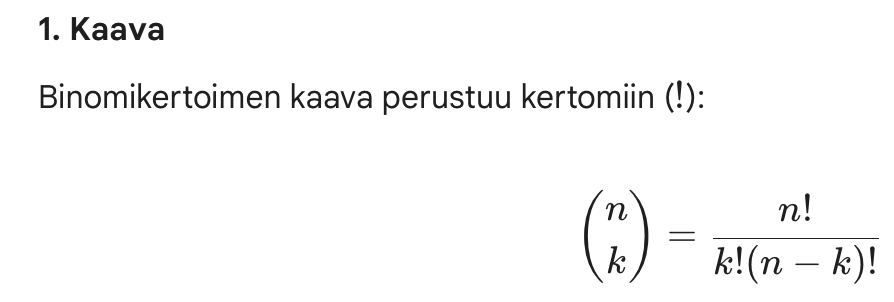
\includegraphics[keepaspectratio]{images/clipboard-3175951006.png}}

Eli montako eri tapaa on valita tietty joukko (k) isommasta joukosta
(n).

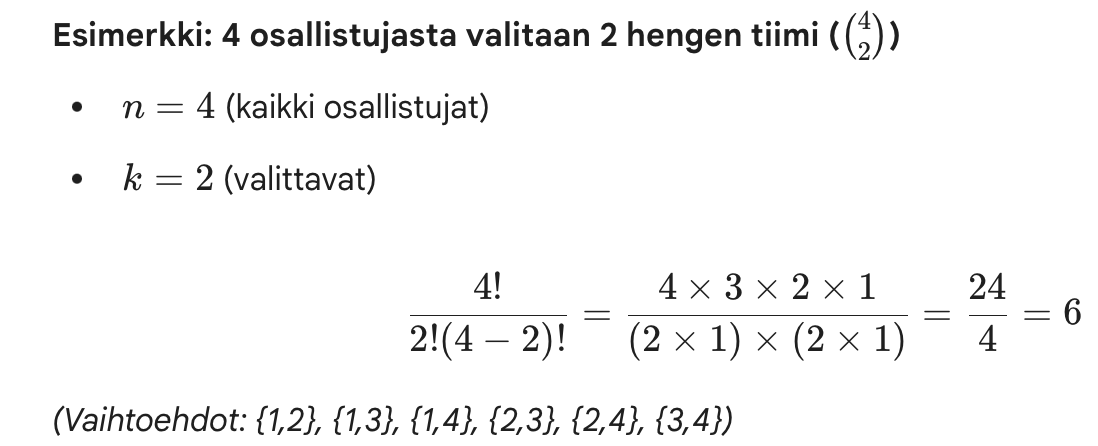
\includegraphics[width=4.55208in,height=\textheight,keepaspectratio]{images/clipboard-2676583055.png}

Permutaatiotestissä lasketaan nimenomaan kombinaatioita

\section{Vektorien laskutoimitukset}\label{vektorien-laskutoimitukset}

Vektori ja yksittäinen arvo

\begin{itemize}
\tightlist
\item
  jokainen vektorin arvo käydään läpi ja tehdään sille sama
  laskutoimitus. Esim. alla vektorin jokaisesta arvosta vähennetään 3 ja
  palautetaan indeksin joka kohdan tulos.
\end{itemize}

\begin{Shaded}
\begin{Highlighting}[]
\FunctionTok{c}\NormalTok{(}\DecValTok{2}\NormalTok{,}\DecValTok{4}\NormalTok{,}\DecValTok{6}\NormalTok{,}\DecValTok{8}\NormalTok{,}\DecValTok{10}\NormalTok{) }\SpecialCharTok{{-}} \DecValTok{3} 
\end{Highlighting}
\end{Shaded}

\begin{verbatim}
[1] -1  1  3  5  7
\end{verbatim}

Kaksi vektoria

\begin{itemize}
\item
  Kahdella yhtä pitkällä vektorilla voi tehdä laskutoimituksia keskenään
\item
  Keskenään lasketaan aina saman indeksinumeron arvo

  \begin{itemize}
  \item
    Jos lasketaan esimerkikis V1 + V2, jossa V1 = c(1,2,3) ja V2 =
    c(2,4,6)

    \begin{itemize}
    \item
      lasketaan 1. V1{[}1{]} + V2{[}1{]} = 1 + 2 = 3
    \item
      2. V1{[}2{]} + V2{[}2{]} = 2 + 4 = 6
    \item
      3. V1{[}3{]} + V2{[}3{]} = 3 + 6 = 9
    \end{itemize}

\begin{Shaded}
\begin{Highlighting}[]
\FunctionTok{c}\NormalTok{(}\DecValTok{1}\NormalTok{,}\DecValTok{2}\NormalTok{,}\DecValTok{3}\NormalTok{) }\SpecialCharTok{+} \FunctionTok{c}\NormalTok{(}\DecValTok{2}\NormalTok{,}\DecValTok{4}\NormalTok{,}\DecValTok{6}\NormalTok{)}
\end{Highlighting}
\end{Shaded}

\begin{verbatim}
[1] 3 6 9
\end{verbatim}
  \end{itemize}
\end{itemize}

\section{Summafunktiot: sum(), colSums() ja
rowSums()}\label{summafunktiot-sum-colsums-ja-rowsums}

sum()

\begin{itemize}
\item
  laskee annetun aineiston kaikkien arvojen summan
\item
  Esim dataframessa siis jokaisen solun summa eli kaikki rivit ja kaikki
  sarakkeet
\end{itemize}

colSums()

\begin{itemize}
\item
  laskee annetun aineiston kolumnien summat
\item
  eli, jos datafreimissä on 20 saraketta ja 10 riviä, niin antaa
  vastauksena 20 summaa

  \begin{itemize}
  \tightlist
  \item
    laskee siis sarakkeen 1. 10 arvoa yhteen, sarakkeen 2. 10 arvoa
    yhteen, sarakkeen 3. 10 arvoa yhteen jne.
  \end{itemize}
\end{itemize}

rowSums()

\begin{itemize}
\item
  laskee annetun aineiston rivien summat

  jos datafreimissä 20 saraketta ja 10 riviä, niin antaa vastauksena 10
  summaa

  \begin{itemize}
  \tightlist
  \item
    laskee rivin 1. 20 arvoa yhteen, rivin 2. 20 arvoa yhteen, rivin 3.
    20 arvoa yhteen jne.
  \end{itemize}
\end{itemize}

nrow()

\begin{itemize}
\tightlist
\item
  kertoo montako riviä on annetussa aineistossa
\end{itemize}

ncol()

\begin{itemize}
\tightlist
\item
  kertoo montako saraketta on annetussa aineistossa
\end{itemize}

\section{Matemaattisia
operaattoreita}\label{matemaattisia-operaattoreita}

\begin{itemize}
\item
  \texttt{abs(x)}: laskee itseisarvon\textbar x\textbar.
\item
  \texttt{sqrt(x)}: laskee neliöjuuren~√x.
\item
  \texttt{log(x)}: laskee logaritmin~x~jossa luonnollinen luku~e~on
  perustana.
\item
  \texttt{log(x,\ base\ =\ a)}: laskee logaritmin~x~jossa luku~a~on
  perustana.
\item
  \texttt{a\^{}x}: laskee a potenssiin x
\item
  \texttt{exp(x)}: laskee e potenssiin x
\item
  \texttt{sin(x)}:laskee sin(x).
\item
  \texttt{sum(x)}: kun~\texttt{x}~on vektori~x=(x1,x2,x3,\ldots,xn),
  laskee summan sen elementeistä~\texttt{x}:~∑ni=1xi.
\item
  \texttt{prod(x)}: kun~\texttt{x}~on vektori~x=(x1,x2,x3,\ldots,xn),
  computes the product of the elements of~\texttt{x}:~∏ni=1xi.
\item
  \texttt{pi}: a built-in variable with value~π, the ratio of the
  circumference of a circle to its diameter.
\item
  \texttt{x\ \%\%\ a}: computes~x~modulo~a.
\item
  \texttt{factorial(x)}: laskee kertoman~x!.
\item
  \texttt{choose(n,k)}: laskee kombinaatiot~(nk).

  Selitykset ovat suoraan Modern statistics with R kirjasta (Thulin
  (2024)).
\end{itemize}

\chapter{Tekstikomentoja}\label{tekstikomentoja}

\section{Tekstin kirjoittaminen ja .txt tekstitiedoston
luominen}\label{tekstin-kirjoittaminen-ja-.txt-tekstitiedoston-luominen}

\begin{Shaded}
\begin{Highlighting}[]
\NormalTok{teksti }\OtherTok{\textless{}{-}} \FunctionTok{c}\NormalTok{(}\StringTok{"Tehtävämoniste 1 {-} 4 luokkalaisille"}\NormalTok{, }
            \StringTok{"Ratkaise seuraavat 10 tehtävää:"}\NormalTok{, }
            \StringTok{""}\NormalTok{, }
            \StringTok{"Tehtävä 1:"}\NormalTok{, }
            \StringTok{""}\NormalTok{)}

\FunctionTok{writeLines}\NormalTok{(teksti, }\StringTok{"matikkatehtavat.txt"}\NormalTok{)}
\end{Highlighting}
\end{Shaded}

\begin{itemize}
\item
  Jokainen vektorin alkio menee \textbf{writeLines()} funktiolla
  tallennettuun tiedostoon omalle riville

  \begin{itemize}
  \item
    eli pilkulla erottamalla saa tehtyä rivinvaihdon
  \item
    teksti kohtaan vektori, josta teksti / sisältö haetaan ja pilkun
    jälkeen uuden tiedoston nimi
  \item
    tyhjän rivin saa tehtyä merkkaamalla vektoriin alkioksi pelkät
    hipsut ``\,'' , kuten riveillä 3 ja 5
  \end{itemize}
\end{itemize}

\section{Merkkijonojen yhdistäminen Paste()
funktiolla}\label{merkkijonojen-yhdistuxe4minen-paste-funktiolla}

\begin{Shaded}
\begin{Highlighting}[]
\NormalTok{tallennettu }\OtherTok{\textless{}{-}} \DecValTok{120}

\NormalTok{paste}\OtherTok{\textless{}{-}} \FunctionTok{paste}\NormalTok{(}\StringTok{"jotakin"}\NormalTok{, }\StringTok{"jotakin"}\NormalTok{, tallennettu)}
\NormalTok{paste0 }\OtherTok{\textless{}{-}} \FunctionTok{paste0}\NormalTok{(}\StringTok{"jotakin"}\NormalTok{, }\StringTok{"jotakin"}\NormalTok{, tallennettu) }

\FunctionTok{print}\NormalTok{(paste)}
\end{Highlighting}
\end{Shaded}

\begin{verbatim}
[1] "jotakin jotakin 120"
\end{verbatim}

\begin{Shaded}
\begin{Highlighting}[]
\FunctionTok{print}\NormalTok{(paste0)}
\end{Highlighting}
\end{Shaded}

\begin{verbatim}
[1] "jotakinjotakin120"
\end{verbatim}

\begin{itemize}
\item
  paste funktiolla saa siis yhdistettyä useita tekstijonoja yhdeksi
  tekstijonoksi

  \begin{itemize}
  \item
    \textbf{paste()} laittaa oletksena välilyönnin joukkojen väliin
  \item
    \textbf{paste0()} ei laita välilyöntiä väleihin
  \item
  \end{itemize}
\end{itemize}

Voi myös hyödyntää esimerkiksi jos for loopilla luo juoksevan nimeämisen
tiedostoille. Alla olevassa esimerkissä siirretään kansioita uuteen
kansioon. For loopin avulla saadaan haettua kaikki Koulu(1-7) nimiset
kansiot. Siinä siis paste0() funktiolla yhdistetään ``Koulu ja juokseva
numero yhdeksi kirjainjonoksi Koulu1, Koulu2, Koulu3 jne.

\begin{Shaded}
\begin{Highlighting}[]
\ControlFlowTok{for}\NormalTok{ (i }\ControlFlowTok{in} \DecValTok{1}\SpecialCharTok{:}\DecValTok{7}\NormalTok{) \{}
\NormalTok{  vanha\_nimi }\OtherTok{\textless{}{-}} \FunctionTok{paste0}\NormalTok{(}\StringTok{"Koulu"}\NormalTok{, i)}
\NormalTok{  uusi\_nimi }\OtherTok{\textless{}{-}} \FunctionTok{file.path}\NormalTok{(uusi\_paakansio, vanha\_nimi)}
  
  \CommentTok{\# file.rename siirtää koko kansion sisältöineen päivineen}
  \FunctionTok{file.rename}\NormalTok{(}\AttributeTok{from =}\NormalTok{ vanha\_nimi, }\AttributeTok{to =}\NormalTok{ uusi\_nimi)}
\NormalTok{\}}
\end{Highlighting}
\end{Shaded}

\section{PDF tiedoston luominen ja siihen asioiden
kirjoittaminen}\label{pdf-tiedoston-luominen-ja-siihen-asioiden-kirjoittaminen}

PDF luodaan komennolla \textbf{pdf()}

\begin{Shaded}
\begin{Highlighting}[]
\FunctionTok{pdf}\NormalTok{(}\StringTok{"VisualisointiDiagnoosiTeht.pdf"}\NormalTok{, }\AttributeTok{width =} \DecValTok{8}\NormalTok{, }\AttributeTok{height =} \DecValTok{6}\NormalTok{)}
\end{Highlighting}
\end{Shaded}

\begin{itemize}
\tightlist
\item
  tämän jälkeisille riveille laitetun koodin tulokset tulostuvat
  kyseiseen pdf tiedostoon
\end{itemize}

PDF:n kirjoitus täytyy sulkea komennolla \textbf{dev.off()}

\begin{Shaded}
\begin{Highlighting}[]
\CommentTok{\# Suljetaan PDF:n kirjoitus }
\FunctionTok{dev.off}\NormalTok{()}
\end{Highlighting}
\end{Shaded}

Ennen \textbf{pdf()} komentoa voi olla järkevää laittaa while looppi,
joka varmistaa, että kaikki aiemmat PDF yhteydet ovat sulkeutuneet.

\begin{Shaded}
\begin{Highlighting}[]
\CommentTok{\#  Suljetaan mahdolliset aiemmat jumiutuneet PDF{-}yhteydet}
\ControlFlowTok{while}\NormalTok{(}\SpecialCharTok{!}\FunctionTok{is.null}\NormalTok{(}\FunctionTok{dev.list}\NormalTok{())) }\FunctionTok{dev.off}\NormalTok{()}
\end{Highlighting}
\end{Shaded}

\textbf{gridExtra} ja \textbf{grid} pakettiin kuuluvilla komennoilla
saadaan kirjoitettua tekstiä PDF:n

\begin{Shaded}
\begin{Highlighting}[]
\FunctionTok{library}\NormalTok{(gridExtra)}
\FunctionTok{library}\NormalTok{(grid)}

\NormalTok{otsikko2 }\OtherTok{\textless{}{-}} \FunctionTok{textGrob}\NormalTok{(}\StringTok{"Oppimimisen erot klustereittain"}\NormalTok{, }
                    \AttributeTok{gp =} \FunctionTok{gpar}\NormalTok{(}\AttributeTok{fontsize =} \DecValTok{18}\NormalTok{, }\AttributeTok{fontface =} \StringTok{"bold"}\NormalTok{))}

\NormalTok{teksti\_sisalto2 }\OtherTok{\textless{}{-}} \StringTok{"Kuten edellisen sivun kuvaajista nähdään, vaikeimmissa diagnooseissa }
\StringTok{                    }\SpecialCharTok{\textbackslash{}n}\StringTok{ oppimisen kehitys oli suurinta ja helpommissa pienintä."}

\NormalTok{leipateksti2 }\OtherTok{\textless{}{-}} \FunctionTok{textGrob}\NormalTok{(teksti\_sisalto2, }
                        \AttributeTok{x =} \FloatTok{0.1}\NormalTok{, }\CommentTok{\# Aloituskohta vasemmalta (0{-}1)}
                        \AttributeTok{just =} \StringTok{"left"}\NormalTok{, }\CommentTok{\# Tasaus vasempaan reunaan}
                        \AttributeTok{gp =} \FunctionTok{gpar}\NormalTok{(}\AttributeTok{fontsize =} \DecValTok{12}\NormalTok{))}

\FunctionTok{grid.arrange}\NormalTok{(otsikko2, leipateksti2, }\AttributeTok{ncol =} \DecValTok{1}\NormalTok{, }\AttributeTok{heights =} \FunctionTok{c}\NormalTok{(}\FloatTok{0.1}\NormalTok{, }\FloatTok{0.9}\NormalTok{))}
\end{Highlighting}
\end{Shaded}

\begin{itemize}
\item
  \textbf{textGrob()}

  \begin{itemize}
  \item
    ekaan väliin sisällytettävä teksti
  \item
    gp = gpar(fontsize = , fontface = )

    \begin{itemize}
    \tightlist
    \item
      tekstin muotoilut
    \end{itemize}
  \item
    oletuksena piirtää tekstin keskelle (x = 0.5)

    \begin{itemize}
    \tightlist
    \item
      jos merkataan x = 0.1 niin aloittaa tekstin vasemmasta reunasta
    \end{itemize}
  \item
    just = ``left''

    \begin{itemize}
    \tightlist
    \item
      tasataan teksti vasempaan reunaan
    \end{itemize}
  \end{itemize}
\item
  \textbf{grid.arrange()}

  \begin{itemize}
  \item
    tällä piirretään textGrob() funktiolla muotoillut muuttujat PDF
    tiedostoon
  \item
    Syötetään kirjoitettavat muuttujat pilkuilla eroteltuina
  \item
    ncol = 1 -\textgreater{} kertoo sarakkeiden määrän, kun on yksi niin
    teksti tulee sivulle normaalisti yhteen sarakkeeseen
  \item
    heights() -\textgreater{} määrittää muuttujien viemän tilan
    y-akselin suunnassa. Eli toisin sanottuna korkeuden.

    \begin{itemize}
    \item
      Esim. jos heights( 0.1, 0.9)

      \begin{itemize}
      \tightlist
      \item
        Ensimmäinen muuttuja vie 10 \% y-akselista ja toinen 90\%
      \end{itemize}
    \end{itemize}
  \end{itemize}
\end{itemize}

\textbf{print()} komennolla voidaan tulostaa kuva PDF tiedostoon

\begin{Shaded}
\begin{Highlighting}[]
\FunctionTok{print}\NormalTok{(}\FunctionTok{ggplot}\NormalTok{(PerceptualLearnData, }\FunctionTok{aes}\NormalTok{(}\AttributeTok{x =} \FunctionTok{as.factor}\NormalTok{(SelectedDiag), }\AttributeTok{y =}\NormalTok{ Correct)) }\SpecialCharTok{+}
        \CommentTok{\# Piirretään keskiarvopylväät}
        \FunctionTok{stat\_summary}\NormalTok{(}\AttributeTok{fun =} \StringTok{"mean"}\NormalTok{, }\AttributeTok{geom =} \StringTok{"bar"}\NormalTok{, }\AttributeTok{color =} \StringTok{"blue"}\NormalTok{, }\AttributeTok{fill =} \StringTok{"blue"}\NormalTok{, }\AttributeTok{width =} \FloatTok{0.5}\NormalTok{, }\AttributeTok{na.rm =} \ConstantTok{TRUE}\NormalTok{) }\SpecialCharTok{+}
        \CommentTok{\# Lisätään virhejanat (Standard Error)}
        \FunctionTok{stat\_summary}\NormalTok{(}\AttributeTok{fun.data =} \StringTok{"mean\_se"}\NormalTok{, }\AttributeTok{geom =} \StringTok{"errorbar"}\NormalTok{,}\AttributeTok{color =} \StringTok{"red"}\NormalTok{,  }\AttributeTok{width =} \FloatTok{0.3}\NormalTok{,}\AttributeTok{na.rm =} \ConstantTok{TRUE}\NormalTok{) }\SpecialCharTok{+}
        
        \FunctionTok{labs}\NormalTok{(}\AttributeTok{title =} \StringTok{"Oikeiden vastausten osuus diagnooseittain"}\NormalTok{,}
             \AttributeTok{x =} \StringTok{"Diagnoosi"}\NormalTok{,}
             \AttributeTok{y =} \StringTok{"Osuus vastauksista oikein"}\NormalTok{) }\SpecialCharTok{+}
        \FunctionTok{theme\_minimal}\NormalTok{())}
\end{Highlighting}
\end{Shaded}

Jos halutaan tulostaa useampi samankaltainen kuva hiukan muuttuvilla
parametreillä voidaan käyttää for-looppia

\begin{Shaded}
\begin{Highlighting}[]
\FunctionTok{library}\NormalTok{(ggplot2)}
\FunctionTok{library}\NormalTok{(patchwork)}

\NormalTok{datasetti }\OtherTok{\textless{}{-}} \FunctionTok{list}\NormalTok{(vaikeat, helpot, keski)}
\NormalTok{kuvaaja\_lista2 }\OtherTok{\textless{}{-}} \FunctionTok{list}\NormalTok{()}
\NormalTok{nimet }\OtherTok{\textless{}{-}} \FunctionTok{list}\NormalTok{(}\StringTok{"Vaikeat"}\NormalTok{, }\StringTok{"Helpot"}\NormalTok{, }\StringTok{"Keskimääräiset"}\NormalTok{)}

\ControlFlowTok{for}\NormalTok{( i }\ControlFlowTok{in} \DecValTok{1}\SpecialCharTok{:}\FunctionTok{length}\NormalTok{(datasetti))\{}
\NormalTok{  p }\OtherTok{\textless{}{-}} \FunctionTok{ggplot}\NormalTok{(datasetti[[i]], }\FunctionTok{aes}\NormalTok{(}\AttributeTok{x =} \FunctionTok{as.factor}\NormalTok{(Session), }\AttributeTok{y =}\NormalTok{ Correct, }\AttributeTok{fill =}\NormalTok{ Session)) }\SpecialCharTok{+}
    \FunctionTok{stat\_summary}\NormalTok{(}\AttributeTok{fun =} \StringTok{"mean"}\NormalTok{, }\AttributeTok{geom =} \StringTok{"bar"}\NormalTok{, }\AttributeTok{color =} \StringTok{"black"}\NormalTok{, }\AttributeTok{width =} \FloatTok{0.8}\NormalTok{, }\AttributeTok{na.rm =} \ConstantTok{TRUE}\NormalTok{) }\SpecialCharTok{+}
    \FunctionTok{stat\_summary}\NormalTok{(}\AttributeTok{fun.data =} \StringTok{"mean\_se"}\NormalTok{, }\AttributeTok{geom =} \StringTok{"errorbar"}\NormalTok{, }\AttributeTok{color =} \StringTok{"red"}\NormalTok{, }\AttributeTok{width =} \FloatTok{0.3}\NormalTok{, }\AttributeTok{na.rm =} \ConstantTok{TRUE}\NormalTok{) }\SpecialCharTok{+}
    \FunctionTok{labs}\NormalTok{(}\AttributeTok{title =}\NormalTok{ nimet[i], }
         \AttributeTok{x =} \StringTok{"Sessio"}\NormalTok{,}
         \AttributeTok{y =} \StringTok{"Oikeiden diagnoosien osuus"}\NormalTok{) }\SpecialCharTok{+}
    \FunctionTok{theme\_minimal}\NormalTok{() }\SpecialCharTok{+}
    \FunctionTok{theme}\NormalTok{(}\AttributeTok{legend.position =} \StringTok{"none"}\NormalTok{)}
  
\NormalTok{  kuvaaja\_lista2[[i]] }\OtherTok{\textless{}{-}}\NormalTok{ p }
\NormalTok{\}}

\FunctionTok{wrap\_plots}\NormalTok{(kuvaaja\_lista2, }\AttributeTok{ncol =} \DecValTok{3}\NormalTok{)}
\end{Highlighting}
\end{Shaded}

\begin{itemize}
\item
  kuvaaja\_lista2 \textless- list()

  \begin{itemize}
  \tightlist
  \item
    \textbf{list()} komennolla alustetaan kuvaaja\_lista2 muuttuja
    listamuotoiseksi, jolloin sinne voidaan tallettaa asioita listana
  \end{itemize}
\item
  datasetti muuttujaan talletetaan kolme hiukan erilaista data.framea
  listana \textbf{list()} komennolla
\item
  nimet muuttujaan puolestaan datasettien nimet
\item
  for-looppi suorittaa 1 -\textgreater{} datasetin pituus kertoja (tässä
  tapauksessa 3, eli 1:3) sen sisältämän koodin siten, että i tilalle
  asetetaan in jälkeen annetut arvot

  \begin{itemize}
  \item
    eli ensimmäisellä kierroksella i = 1
  \item
    toisella i = 2
  \item
    kolmannella i = 3
  \end{itemize}
\item
  datasetti{[}{[}i{]}{]}

  \begin{itemize}
  \tightlist
  \item
    kaksilla hakasulkeilla viitattuna saadaan listasta datasetti haettua
    indeksinumerolla muuttuja
  \end{itemize}
\item
  p muuttujaan talletetaan aina luotu kuva ja se puolestaan talletetaan
  kuvaaja\_lista2:n

  \begin{itemize}
  \tightlist
  \item
    kuvaaja\_lista2{[}{[}i{]}{]} \textless- p
  \end{itemize}
\item
  wrap\_plots(kuvaaja\_lista2, ncol = 3)

  \begin{itemize}
  \item
    wrap\_plots() funktiolla piirretään kuvaajat

    \begin{itemize}
    \tightlist
    \item
      kuuluu patchwork pakettiin
    \end{itemize}
  \item
    ncol= määrittää sarakkeiden määrän. Jos se on kolme niin yhdelle
    riville tulee kolme kuvaa vierekkäin
  \item
  \end{itemize}
\end{itemize}

\chapter{Varmuuskopiointi}\label{varmuuskopiointi}

\section{Git ja github}\label{git-ja-github}

\begin{Shaded}
\begin{Highlighting}[]
\NormalTok{usethis}\SpecialCharTok{::}\FunctionTok{use\_git}\NormalTok{()}
\end{Highlighting}
\end{Shaded}

Luo olemassa olevalle R-projektille git repositorion

\begin{itemize}
\item
  uutta projektia luodessa voi rastittaa saman heti alkuun
\item
  git repositorioon voi tallentaa varmuuskopion aina kun haluaa

  \begin{itemize}
  \tightlist
  \item
    se tehdään yläoikealta git välilehdeltä valitsemalla tehdyt
    muutokset ja painamalla commit
  \end{itemize}
\end{itemize}

Kun on luonut tunnukset GitHubiin voi projektin tallettaa tililleen
pilveen. Paikallinen git täytyy ensin yhdistää githubiin luomalla github
token ja lisäämällä se Rstudioon. Github token toimii salasanana. Github
suosittelee, että token on voimassa vain määräajan esim. 30 tai 90
päivää, mutta laitoin sen jatkuvasti voimassa olevaksi, koska en halua
säätää sen kanssa koko ajan. Alla skripti, jolla pääsee githubin
sivuille luomaan tokenin ja sen jälkeen lisäämään sen rstudioon. Token
tarvitsee lisätä vain yhteen projektiin rstudiossa ja se toimii sen
jälkeen kaikissa. Lisätäkseen projektin gitiin ja githubiin täytyy ajaa
komennot \textbf{usethis::use\_git()} ja \textbf{usethis::use\_github()}

\begin{Shaded}
\begin{Highlighting}[]
\ControlFlowTok{if}\NormalTok{(}\SpecialCharTok{!}\FunctionTok{require}\NormalTok{(usethis)) }\FunctionTok{install.packages}\NormalTok{(}\StringTok{"usethis"}\NormalTok{)}
\FunctionTok{library}\NormalTok{(usethis)}

\CommentTok{\# Tämä avaa selaimesi suoraan GitHubin oikealle sivulle}
\FunctionTok{create\_github\_token}\NormalTok{()}

\ControlFlowTok{if}\NormalTok{(}\SpecialCharTok{!}\FunctionTok{require}\NormalTok{(gitcreds)) }\FunctionTok{install.packages}\NormalTok{(}\StringTok{"gitcreds"}\NormalTok{)}
\FunctionTok{library}\NormalTok{(gitcreds)}

\CommentTok{\# Aja tämä ja liitä kopioimasi token (koodi) pyydettäessä konsoliin}
\FunctionTok{gitcreds\_set}\NormalTok{()}

\CommentTok{\# Tämä komento hoitaa kaiken: luo GitHubiin uuden kansion (repository) }
\CommentTok{\# ja lähettää tiedostosi sinne.}
\NormalTok{usethis}\SpecialCharTok{::}\FunctionTok{use\_github}\NormalTok{()}


\CommentTok{\# Kun luo uuden projektin niin alla olevat komennot täytyy ajaa, jotta git ja github toimivat. Tokenia ei tarvitse ajaa uudestaan. }
\CommentTok{\# usethis::use\_git() ja usethis::use\_github().}
\end{Highlighting}
\end{Shaded}

\section{.gitignore}\label{gitignore}

\begin{itemize}
\item
  Gemini suositteli lisäämään alla olevat asiat gitignore tiedostoon

  \begin{itemize}
  \item
    sieltä määritetään, mitä ei varmuuskopioida
  \item
    Turhia asioita ei kannata varmuuskopioida, jotta git pysyy selkeänä
    ja sulavana
  \end{itemize}
\end{itemize}

\begin{Shaded}
\begin{Highlighting}[]
\NormalTok{.Rproj.user}
\NormalTok{.Rhistory}
\NormalTok{.RData}
\NormalTok{.httr}\SpecialCharTok{{-}}\NormalTok{oauth}
\NormalTok{.DS\_Store}
\NormalTok{.quarto}
\SpecialCharTok{/}\NormalTok{.quarto}\SpecialCharTok{/}
\ErrorTok{**/*}\NormalTok{.quarto\_ipynb}
\NormalTok{\_book}\SpecialCharTok{/}
\NormalTok{\_site}\SpecialCharTok{/}
\NormalTok{site\_libs}\SpecialCharTok{/}
\end{Highlighting}
\end{Shaded}

\section{Quarto-kirja nettisivuksi githubin
avulla}\label{quarto-kirja-nettisivuksi-githubin-avulla}

Quarto kirjan saa githubin kautta nettisivuksi muutamalla simppelillä
työvaiheella. Aivan ensiksi quarto-kirjan projektikansion täytyy löytyä
githubista eli suorita \textbf{usethis::use\_git()} ja
\textbf{usethis::use\_github()} mikäli et ole niitä jo tehnyt. Ensiksi
täytyy lisätä quarto.yml tiedostoon: ``\textbf{output-dir: docs}''. Se
lisää projektiin kansion docs, jota käytetään nettisivun lähdekansiona.

\begin{Shaded}
\begin{Highlighting}[]
\NormalTok{project}\SpecialCharTok{:}
\NormalTok{  type}\SpecialCharTok{:}\NormalTok{ book}
\NormalTok{  output}\SpecialCharTok{{-}}\NormalTok{dir}\SpecialCharTok{:}\NormalTok{ docs }
\end{Highlighting}
\end{Shaded}

Sen lisäksi .gitignore tiedostosta täytyy poistaa tai kommentoida
muutama asia, jotta docs kansioon, gitiin ja githubiin tallentuu mukaan
tarvittavat tiedostot. .gitignoresta täytyy poistaa tai kommentoida
\textbf{book/}, \textbf{site/} ja \textbf{site\_libs/}. Ne ovat
kirjastotiedostoja ja lisättiin gitignoreen alunperin, koska niitä
tallentuu aina renderöidessä paljon ja voivat hidastaa gitin toimintaa.
Nettisivuja tehdessä niidenkin tiedostojen täytyy siirtyä gitiin ja
githubiin, joten siksi ne poistetaan .gitignore tiedostosta.

Kirjani .gitignore tiedosto näyttää tältä:

\begin{Shaded}
\begin{Highlighting}[]
\NormalTok{.Rproj.user}
\NormalTok{.Rhistory}
\NormalTok{.RData}
\NormalTok{.httr}\SpecialCharTok{{-}}\NormalTok{oauth}
\NormalTok{.DS\_Store}
\NormalTok{.quarto}

\SpecialCharTok{/}\NormalTok{.quarto}\SpecialCharTok{/}
\ErrorTok{**/*}\NormalTok{.quarto\_ipynb}
\CommentTok{\# \_book/}
\CommentTok{\# \_site/}
\CommentTok{\# site\_libs/}
\NormalTok{.positai}
\end{Highlighting}
\end{Shaded}

Noiden valmistelujen lisäksi projektikansioon täytyy lisätä tiedosto
``\textbf{.nojekyll}''. Se lisätään, koska github pyrkii muotoilemaan
nettisivut jekyll tyylillä, joka puolestaan estää quarton muotoilujen
käyttämisen. .nojekyll tiedosto kertoo githubille, että käytetään
quarton muotoiluja ja silloin nettisivut saa näyttämään samalta, kuin
html preview tilassa. Tässä on tärkeää muistaa renderöidä projekti
tiedoston luomisen jälkeen, koska muuten tiedosto ei generoidu myös docs
kansioon, jossa sitä tarvitaan.

\begin{Shaded}
\begin{Highlighting}[]
\SpecialCharTok{\textgreater{}} \FunctionTok{file.create}\NormalTok{(}\StringTok{".nojekyll"}\NormalTok{)}
\end{Highlighting}
\end{Shaded}

.nojekyll on piilotiedosto eli sitä ei tarvitse ihmetellä, jos se ei näy
files näkymässä. Voit tarkistaa onnistuitko luomaan sen komennolla
\textbf{list.files()}

\begin{Shaded}
\begin{Highlighting}[]
\SpecialCharTok{\textgreater{}} \FunctionTok{list.files}\NormalTok{(}\AttributeTok{all.files =} \ConstantTok{TRUE}\NormalTok{, }\AttributeTok{pattern =} \StringTok{"jekyll"}\NormalTok{)}
\end{Highlighting}
\end{Shaded}

Mikäli muotoilut eivät mene oikein voidaan ajaa terminaalissa komennot
``git add docs/'' ja ``git add -f docs/site\_libs/'', jotka pakottava
lisäämään gitiin site\_libs/ ja docs/ tiedostot. \textbf{Tee nämä vain
jos kohtaat ongelmia eli muotoilut nettisivuilla eivät näytä oikealta.}

\begin{Shaded}
\begin{Highlighting}[]
\CommentTok{\# ajetaan terminaalissa }
\NormalTok{git add docs}\SpecialCharTok{/}
\NormalTok{git add }\SpecialCharTok{{-}}\NormalTok{f docs}\SpecialCharTok{/}\NormalTok{site\_libs}\SpecialCharTok{/}
\end{Highlighting}
\end{Shaded}

Kun on tehnyt määritykset quarto.yml ja .gitignore tiedostoihin on
tärkeää muistaa renderöidä koko projekti html muodossa. Sen jälkeen
täytyy commitata muutokset gitiin ja sitten vielä pushata ne githubiin.
Tämän jälkeen voidaan siirtyä githubiin viimeistelemään nettisivu.

Työvaiheet ovat siis: Määritykset yml ja gitignore tiedostoihin
--\textgreater{} luo .nojekyll tiedosto --\textgreater{} renderöi
projekti --\textgreater{} commit -\textgreater{} push

Mene githubiin ja avaa sieltä kyseisen projektin repositorio. Actions
välilehdeltä voi tarkistaa onko viimeisin push komento jo suoritettuna
ja ajan tasalla. Sen kohdalla on punainen pallo, jos on ongelmaa,
keltainen jos suorittaminen on kesken ja vihreä jos kaikki on valmiina.
Mene repositorion settings välilehdelle ja valitse vasemmalla reunalla
olevasta listasta Pages.

\begin{figure}[H]

{\centering \pandocbounded{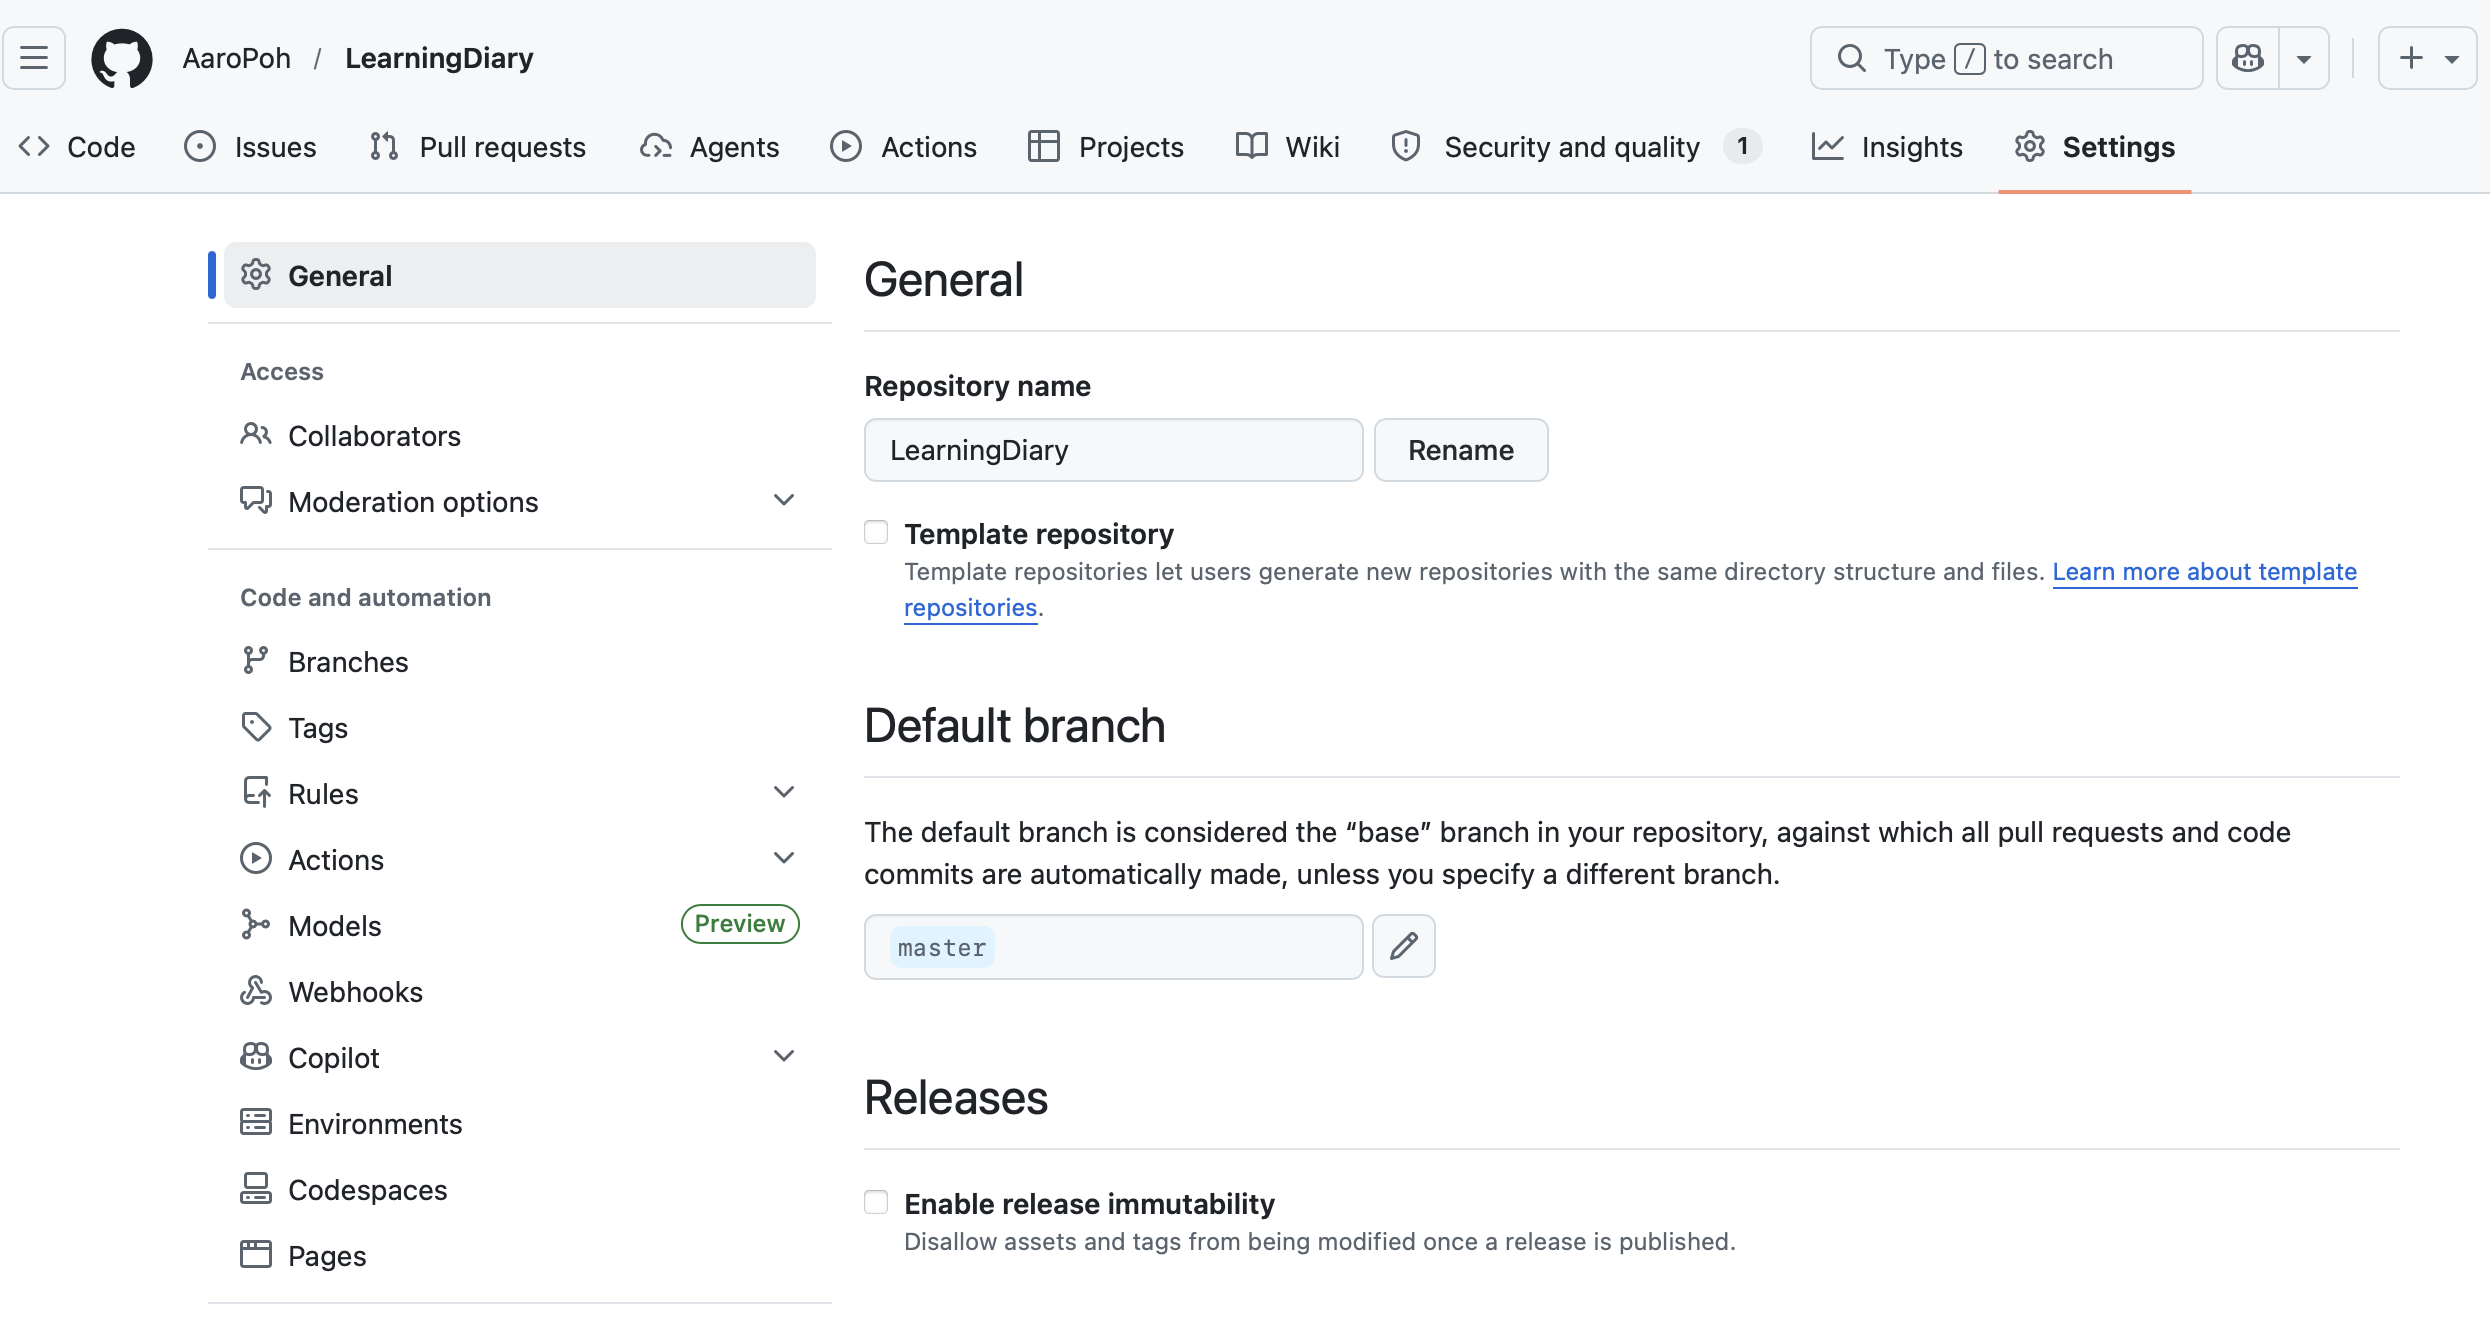
\includegraphics[keepaspectratio]{R_komentoja/images/clipboard-915949178.png}}

}

\caption{}

\end{figure}%

Pages sivulla build and deployement kohdalla säilytä tai valitse source
kohtaan deploy from a branch (Minulla se oli jo valmiiksi siinä). Sitten
valitse branch kohtaan master ja folder kohtaan docs ja paina save. Sen
myötä sinulle täytyisi syntyä nettisivut muodossa
``https://käyttäjänimi.github.io/ProjektiRepositorio/''

\pandocbounded{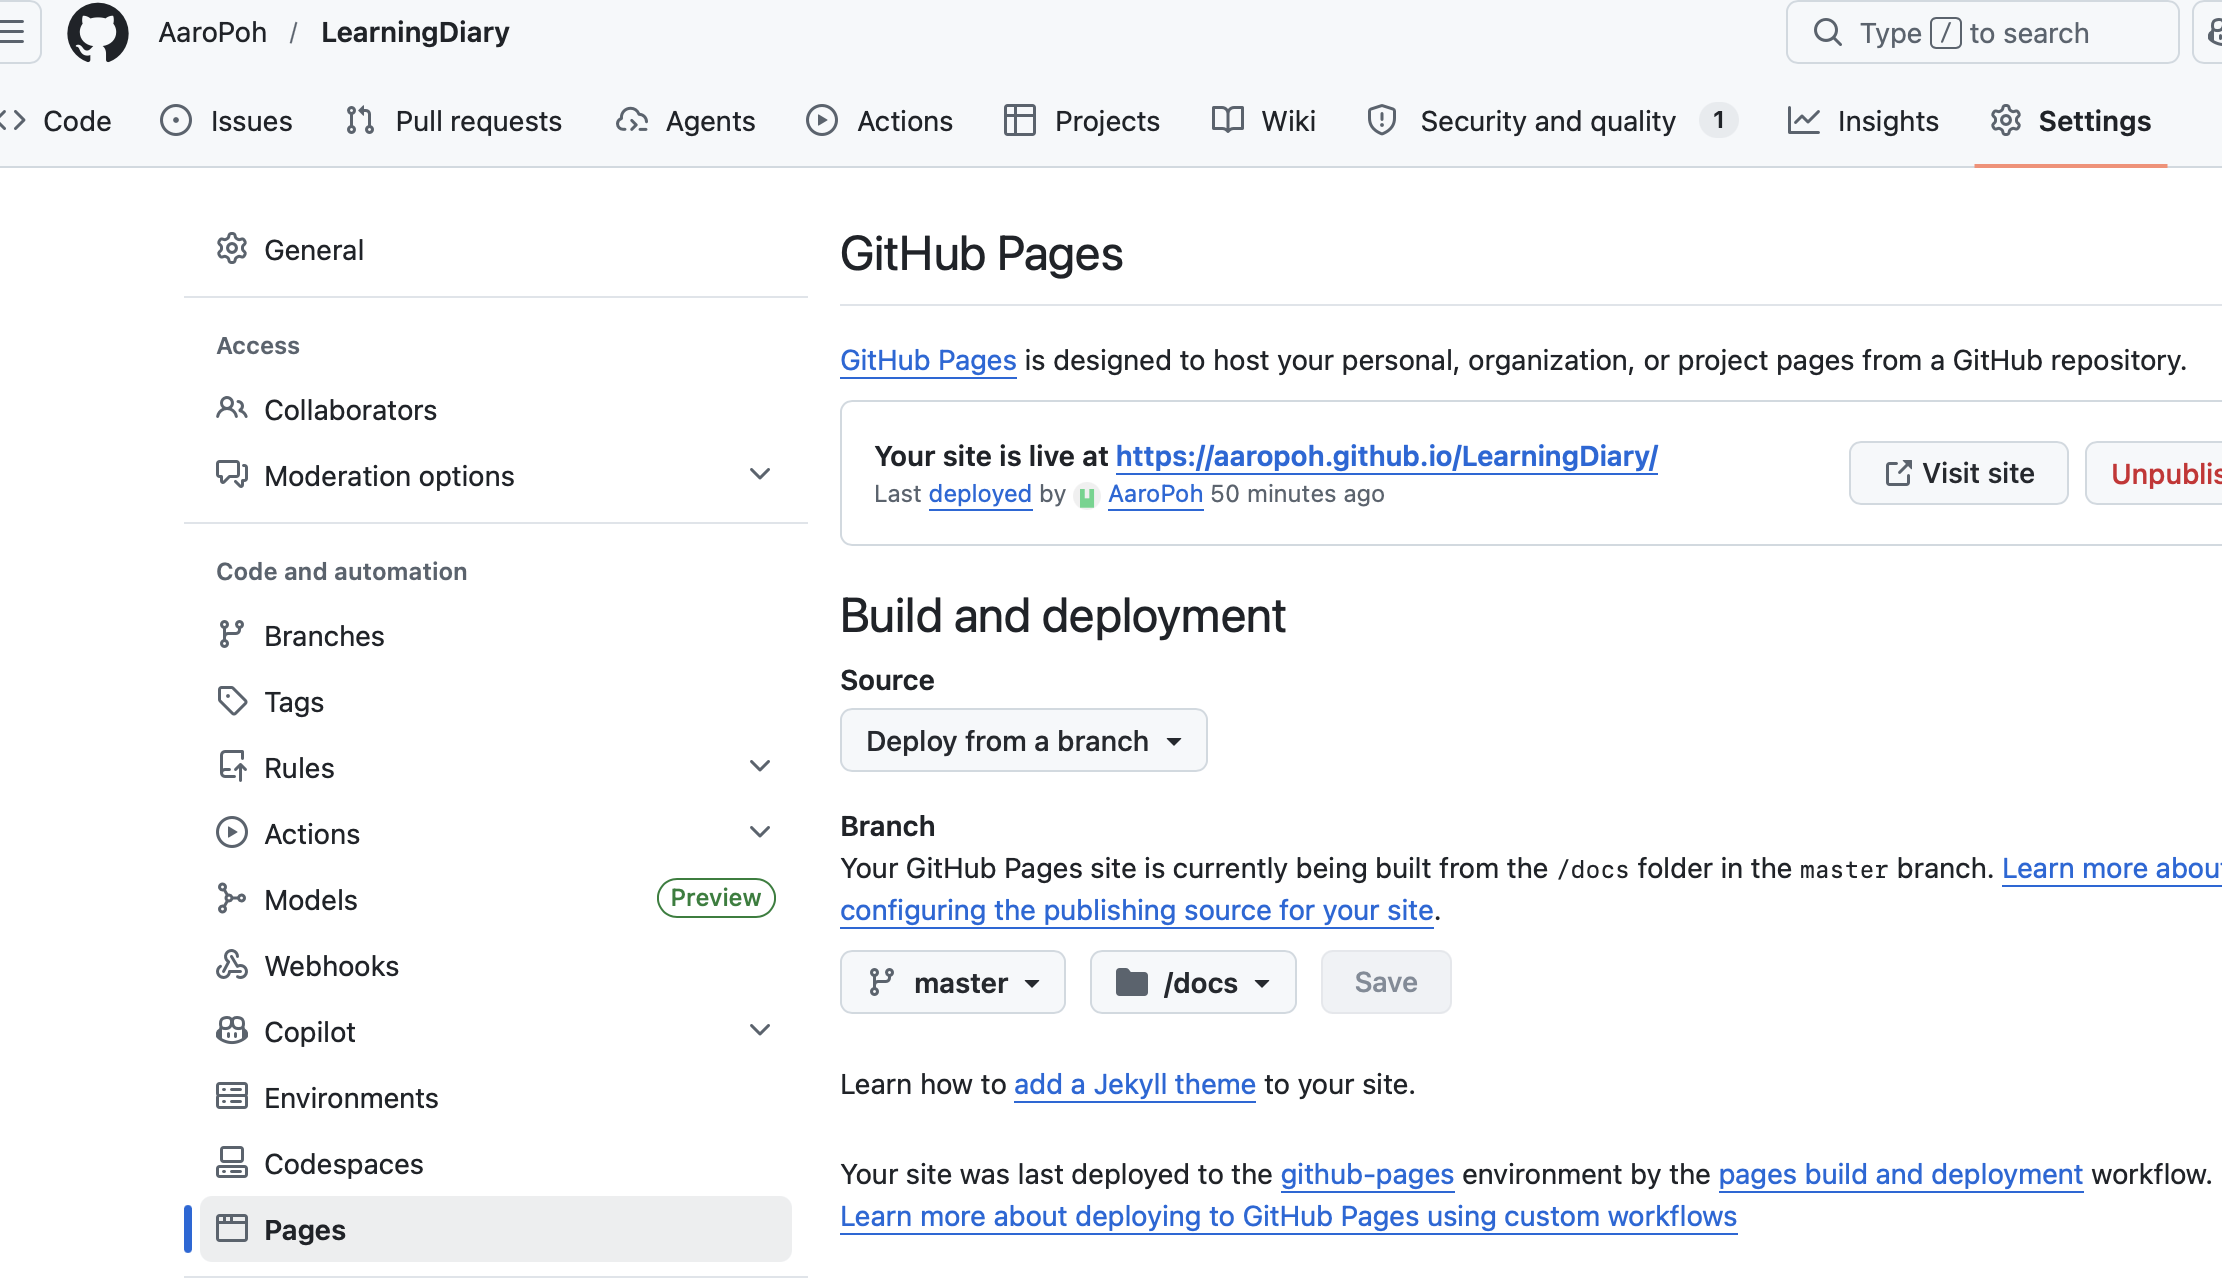
\includegraphics[keepaspectratio]{R_komentoja/images/clipboard-2812852038.png}}

\chapter{Indeksointi / subsetting}\label{indeksointi-subsetting}

Kun käyttää hakasulkeita {[}{]}, antaa R-kielelle ohjeen poimia tietyn
osan datasta. Toisin sanottuna indeksoinnilla saa poimittua mistä vain
datasta osajoukon. Indeksointia on kahta päätyyppiä:

\section{Numeerinen indeksointi}\label{numeerinen-indeksointi}

Kerrotaan suoraan havainnon järjestysnumero.

\textbf{data{[}1{]}} Poimii indeksin ensimmäisen arvon

\begin{Shaded}
\begin{Highlighting}[]
\NormalTok{data }\OtherTok{\textless{}{-}} \FunctionTok{c}\NormalTok{(}\DecValTok{2}\NormalTok{,}\DecValTok{4}\NormalTok{,}\DecValTok{6}\NormalTok{,}\DecValTok{8}\NormalTok{,}\DecValTok{10}\NormalTok{)}

\NormalTok{data[}\DecValTok{1}\NormalTok{]}
\end{Highlighting}
\end{Shaded}

\begin{verbatim}
[1] 2
\end{verbatim}

\textbf{data{[}1:10{]}} poimii indeksin arvot 1-10

\begin{Shaded}
\begin{Highlighting}[]
\NormalTok{data }\OtherTok{\textless{}{-}} \FunctionTok{c}\NormalTok{(}\FunctionTok{seq}\NormalTok{(}\DecValTok{0}\NormalTok{,}\DecValTok{100}\NormalTok{, }\AttributeTok{by =} \DecValTok{5}\NormalTok{))}
\NormalTok{data[}\DecValTok{1}\SpecialCharTok{:}\DecValTok{10}\NormalTok{]}
\end{Highlighting}
\end{Shaded}

\begin{verbatim}
 [1]  0  5 10 15 20 25 30 35 40 45
\end{verbatim}

\textbf{data{[}15:length(data){]}}

\begin{itemize}
\item
  poimii indeksin arvot 15 alkaen loppuun asti
\item
  length(data) palauttaa siis indeksin päätepisteen
\end{itemize}

\begin{Shaded}
\begin{Highlighting}[]
\NormalTok{data }\OtherTok{\textless{}{-}} \FunctionTok{c}\NormalTok{(}\FunctionTok{seq}\NormalTok{(}\DecValTok{0}\NormalTok{,}\DecValTok{100}\NormalTok{, }\AttributeTok{by =} \DecValTok{5}\NormalTok{))}
\NormalTok{data[}\DecValTok{15}\SpecialCharTok{:}\FunctionTok{length}\NormalTok{(data)]}
\end{Highlighting}
\end{Shaded}

\begin{verbatim}
[1]  70  75  80  85  90  95 100
\end{verbatim}

\textbf{data{[}length(data){]}}

\begin{itemize}
\tightlist
\item
  poimii vain indeksin viimeisen arvon eli 10
\end{itemize}

\begin{Shaded}
\begin{Highlighting}[]
\NormalTok{data }\OtherTok{\textless{}{-}} \FunctionTok{c}\NormalTok{(}\DecValTok{2}\NormalTok{,}\DecValTok{4}\NormalTok{,}\DecValTok{6}\NormalTok{,}\DecValTok{8}\NormalTok{,}\DecValTok{10}\NormalTok{)}
\NormalTok{data[}\FunctionTok{length}\NormalTok{(data)]}
\end{Highlighting}
\end{Shaded}

\begin{verbatim}
[1] 10
\end{verbatim}

\begin{itemize}
\tightlist
\item
\end{itemize}

Itsekseen \textbf{length()} näyttää montako montako arvoa vektoriin
kuuluu

\begin{Shaded}
\begin{Highlighting}[]
\NormalTok{data }\OtherTok{\textless{}{-}} \FunctionTok{c}\NormalTok{(}\DecValTok{2}\NormalTok{,}\DecValTok{4}\NormalTok{,}\DecValTok{6}\NormalTok{,}\DecValTok{8}\NormalTok{,}\DecValTok{10}\NormalTok{)}

\FunctionTok{length}\NormalTok{(data)}
\end{Highlighting}
\end{Shaded}

\begin{verbatim}
[1] 5
\end{verbatim}

\textbf{Negatiiviset indeksit} palauttavat koko vektorin lukuunottamatta
näitä indeksejä

\begin{itemize}
\tightlist
\item
  alla 1. ja 2. indeksi jäävät pois
\end{itemize}

\begin{Shaded}
\begin{Highlighting}[]
\NormalTok{data }\OtherTok{\textless{}{-}} \FunctionTok{c}\NormalTok{(}\DecValTok{2}\NormalTok{,}\DecValTok{4}\NormalTok{,}\DecValTok{6}\NormalTok{,}\DecValTok{8}\NormalTok{,}\DecValTok{10}\NormalTok{)}

\NormalTok{data[}\FunctionTok{c}\NormalTok{(}\SpecialCharTok{{-}}\DecValTok{1}\NormalTok{,}\SpecialCharTok{{-}}\DecValTok{2}\NormalTok{)]}
\end{Highlighting}
\end{Shaded}

\begin{verbatim}
[1]  6  8 10
\end{verbatim}

Hyvönen et al. (2018)

\section{Looginen indeksointi}\label{looginen-indeksointi}

Ei anneta tarkkaa järjestysnumeroa, vaan ehto, jonka on täytyttävä.

\begin{itemize}
\tightlist
\item
  \textbf{data{[}data \textgreater{} 5{]}} poimii kaikki arvot, jotka
  ovat suurempia kuin 5
\end{itemize}

\begin{Shaded}
\begin{Highlighting}[]
\NormalTok{data }\OtherTok{\textless{}{-}} \FunctionTok{c}\NormalTok{(}\DecValTok{2}\NormalTok{,}\DecValTok{4}\NormalTok{,}\DecValTok{6}\NormalTok{,}\DecValTok{8}\NormalTok{,}\DecValTok{10}\NormalTok{)}
\NormalTok{data[data }\SpecialCharTok{\textgreater{}} \DecValTok{5}\NormalTok{]}
\end{Highlighting}
\end{Shaded}

\begin{verbatim}
[1]  6  8 10
\end{verbatim}

Kun laittaa hakasulkeiden sisään ehdon, kuten data \textgreater{} 5, R
tekee taustalla näkymättömän listan, joka koostuu vain sanoista TRUE ja
FALSE

\begin{itemize}
\item
  Toimii käytännössä näin:

  \begin{itemize}
  \item
    R käy jokaisen luvun läpi ja antaa sille leiman:

    \begin{itemize}
    \item
      Luku on ehdon sisällä --\textgreater{} TRUE
    \item
      luku on ehdon ulkopuolella -\textgreater{} FALSE
    \end{itemize}
  \item
    komento palauttaa kaikki TRUE arvot
  \end{itemize}
\end{itemize}

Loogisen indeksoinnin voi tehdä myös \textbf{subset()} funktiolla

\begin{Shaded}
\begin{Highlighting}[]
\NormalTok{data }\OtherTok{\textless{}{-}} \FunctionTok{c}\NormalTok{(}\DecValTok{2}\NormalTok{,}\DecValTok{4}\NormalTok{,}\DecValTok{6}\NormalTok{,}\DecValTok{8}\NormalTok{,}\DecValTok{10}\NormalTok{)}

\FunctionTok{subset}\NormalTok{(data, data }\SpecialCharTok{\textgreater{}} \DecValTok{5}\NormalTok{)   }
\end{Highlighting}
\end{Shaded}

\begin{verbatim}
[1]  6  8 10
\end{verbatim}

subset(data, ehto)

\begin{itemize}
\item
  data kohtaan muuttuja, josta halutaan osajoukko
\item
  ehto kohtaan ehto, jonka mukaan osajoukko määritellään.
\end{itemize}

\textbf{\%in\%} operaattori

\begin{itemize}
\item
  ``kuuluu joukkoon'' operaattori
\item
  tarkistaa löytyykö annetusta aineistosta arvot ja palauttaa ne TRUE ja
  FALSE arvoina
\end{itemize}

\begin{Shaded}
\begin{Highlighting}[]
\NormalTok{vaikeimmat }\OtherTok{\textless{}{-}}\NormalTok{ oikeinbydiagnoosi}\SpecialCharTok{$}\NormalTok{SelectedDiag[oikeinbydiagnoosi}\SpecialCharTok{$}\NormalTok{Correct }\SpecialCharTok{\textless{}} \FloatTok{0.6884807}\NormalTok{]}

\NormalTok{vaikeat }\OtherTok{\textless{}{-}} \FunctionTok{subset}\NormalTok{(PerceptualLearnData, SelectedDiag }\SpecialCharTok{\%in\%}\NormalTok{ vaikeimmat)}

\FunctionTok{aggregate}\NormalTok{(Correct }\SpecialCharTok{\textasciitilde{}}\NormalTok{ Session, }\AttributeTok{data =}\NormalTok{ vaikeat, }\AttributeTok{FUN =}\NormalTok{ mean)}
\end{Highlighting}
\end{Shaded}

\begin{itemize}
\tightlist
\item
  koodi tarkistaa PerceptualLearnData datasetin sarakkeen SelectedDiag
  sisältä mitkä kaikki ovat vastaavia kuin vaikeimmat muuttujaan
  määritellyt arvot. Sitten subset funktio tallettaa uuden datasetin,
  jossa SelectedDiag sarakkeessa on vain vaikeimmat ehdon täyttäneet
  arvot.
\end{itemize}

Ei kuulu joukkoon eli !\%in\%

\begin{itemize}
\tightlist
\item
  huutomerkillä (!) eli looogisella ei operaattorilla voi muuntaa kuuluu
  joukkoon operaattorista \%in\% ei kuulu joukkoon operaattorin !\%in\%
\end{itemize}

\section{Kaksiulotteinen indeksi}\label{kaksiulotteinen-indeksi}

Indeksointi sana tulee siitä, että jokaisella tiedonpalasella on oma
``osoitteensa'' eli indeksi.

\begin{itemize}
\item
  Yksiulotteisessa datassa vain yksi indeksi:~data{[}rivi{]}.
\item
  Kaksiulotteisessa datassa~(kuten taulukko tai data.frame) on kaksi
  indeksiä:~data{[}rivi, sarake{]}
\end{itemize}

\section{Yhdet vs.~kahdet
hakasulkeet}\label{yhdet-vs.-kahdet-hakasulkeet}

Yksinkertaiset hakasulkeet {[}{]}

\begin{itemize}
\item
  Yksittäiset sulkeet palauttavat aina saman tyyppisen olion kuin
  alkuperäinen on, mutta pienempänä. Jos leikkaat palan listasta, saat
  \textbf{pienemmän listan}.

  \begin{itemize}
  \tightlist
  \item
    Tulos: Alilista (sub-list).
  \end{itemize}
\end{itemize}

Tuplahakasulkeet {[}{[}{]}{]} (Sisältö)

\begin{itemize}
\tightlist
\item
  Tuplahakasulkeet ``murtavat'' rakenteen ja hakevat sieltä pelkän
  sisällön.
\end{itemize}

\chapter{Funktion luominen ja
kutsuminen}\label{funktion-luominen-ja-kutsuminen}

\section{Funktion luominen:
function()}\label{funktion-luominen-function}

\subsection{Perusrakenne}\label{perusrakenne}

Funktion luominen koostuu neljästä pääosasta:

\begin{Shaded}
\begin{Highlighting}[]
\NormalTok{nimi}\SpecialCharTok{\textless{}}\NormalTok{−}\FunctionTok{function}\NormalTok{(argumentti1, argumentti2)\{ suoritettava koodi\}}
\end{Highlighting}
\end{Shaded}

\begin{itemize}
\item
  Nimi -\textgreater{} Millä nimellä kutsut funktiota (esim.
  laske\_keskiarvo)
\item
  Argumentit -\textgreater{} Mitä tietoa funktio tarvitsee toimiakseen

  \begin{itemize}
  \tightlist
  \item
    argumentit toimivat ``paikan pitäjinä'' eli funktiota käytettäessä
    niihin syötetään mitä tahansa (sopivaa) tietoa ja esim. argumentti1
    kohtaan kirjoitettu tieto menee koodissa joka kohtaan, jossa lukee
    argumentti1
  \end{itemize}
\item
  Runko aaltosulkeiden sisään \{ \} --\textgreater{} Mitä koodia
  suoritetaan.
\item
  Tulostettava arvo --\textgreater{} viimeinen rivi, jonka
  aaltosulkeiden sisällä oleva koodi tuottaa
\end{itemize}

Esimerkkinä tehdään funktio, joka laskee keskiarvon

\begin{Shaded}
\begin{Highlighting}[]
\NormalTok{laske\_keskiarvo }\OtherTok{\textless{}{-}} \ControlFlowTok{function}\NormalTok{(argumentti1)\{}
  
  \FunctionTok{sum}\NormalTok{(argumentti1)}\SpecialCharTok{/}\FunctionTok{length}\NormalTok{(argumentti1)}
\NormalTok{  \}}

\FunctionTok{laske\_keskiarvo}\NormalTok{(}\FunctionTok{c}\NormalTok{(}\DecValTok{2}\NormalTok{,}\DecValTok{4}\NormalTok{,}\DecValTok{6}\NormalTok{,}\DecValTok{8}\NormalTok{,}\DecValTok{10}\NormalTok{))}
\end{Highlighting}
\end{Shaded}

\begin{verbatim}
[1] 6
\end{verbatim}

\begin{itemize}
\item
  aaltosulkeiden sisällä olevassa koodissa argumentti1 esiintyy kahdessa
  paikassa. Kun funktiota käytetään niin se sijoittaa argumentti1
  paikalle syötetyn tiedon koodin joka paikkaan, jossa lukee argumentti1

  \begin{itemize}
  \item
    esim jos syöttäisi näin: laske\_keskiarvo(c(2,2))
  \item
    koodi funktion sisällä näyttäisi tältä:

    \begin{itemize}
    \tightlist
    \item
      \{sum(c(2,2))/length(c(2,2)) \}
    \end{itemize}
  \end{itemize}

\begin{Shaded}
\begin{Highlighting}[]
\NormalTok{laske\_keskiarvo }\OtherTok{\textless{}{-}} \ControlFlowTok{function}\NormalTok{(argumentti1)\{}

  \FunctionTok{sum}\NormalTok{(argumentti1)}\SpecialCharTok{/}\FunctionTok{length}\NormalTok{(argumentti1)}
\NormalTok{  \}}

\FunctionTok{laske\_keskiarvo}\NormalTok{(}\FunctionTok{c}\NormalTok{(}\DecValTok{2}\NormalTok{,}\DecValTok{2}\NormalTok{))}
\end{Highlighting}
\end{Shaded}

\begin{verbatim}
[1] 2
\end{verbatim}
\end{itemize}

\subsection{Argumentit}\label{argumentit}

Argumenttejä voi lisätä niin monta kuin haluaa ja kaikki ne samalla
tavalla toimivat ``paikan pitäjinä''

\begin{itemize}
\item
  Niiden järjestyksellä on merkitystä sillä funktiota käytettäessä luvut
  / muuttujat syötetään järjestyksen mukaan. Esim. jos on tehty useita()
  niminen funktio, jossa on kolme argumenttia

  \begin{itemize}
  \item
    useita \textless- function(argumetti1, argumentti2, argumentti3)\{
    koodi \}
  \item
    niin käytettäessä funktiota sulkeisiin ensimmäiseen väliin tuleva
    arvo korvaa ottaa argumentti1:n paikan, toiseen väliin argumentti2:n
    ja kolmanteen väliin argumentti3:n paikan.

    \begin{itemize}
    \item
      useita(10, 15, 20)

      \begin{itemize}
      \tightlist
      \item
        tällöin funktio sijoittaa aaltosulkeissa olevaan koodiin
        jokaiseen kohtaan, jossa lukee argumentti1 arvon 10, argumentti2
        arvon 15 ja argumentti3 arvon 20.
      \end{itemize}
    \end{itemize}
  \end{itemize}
\item
  Argumentteihin voi viitata myös niiden nimellä ja = merkillä. Sillon
  syöttämisen järjestyksellä ei ole merkitystä.

  \begin{itemize}
  \item
    Esim useita( argumentti1 = 20, argumentti3 = 50)
  \item
    tällöin funktio sijoittaa arvon 20 argumentti1:n paikalle ja arvon
    50 argumentti3:n paikalle.
  \end{itemize}
\end{itemize}

\chapter{Sekalaista}\label{sekalaista}

\section{Run-napin luominen
quarto-kirjaan}\label{run-napin-luominen-quarto-kirjaan}

Quarto-kirjaan saa luotua koodinpätkiä, joita käyttäjä pystyy html
muodossa tulostuvassa kirjassa ajamaan run napilla sekä muokkaamaan. PDF
muodossa näkyy vain koodi ilman sen tuottamia tuloksia. Jos palautus
pitää tehdä pdf muodossa kannattaa muuttaa koodinpätkien muoto takaisin
oletukseksi, jotta myös tulokset tulostuvat kirjaan.

Run napin ja interaktiivisten koodinpätkien luomiseen täytyy tehdä
seuraavat asiat:

\begin{itemize}
\item
  Ajetaan terminaalissa komento: quarto add coatless/quarto-webr

\begin{Shaded}
\begin{Highlighting}[]
\NormalTok{quarto add coatless}\SpecialCharTok{/}\NormalTok{quarto}\SpecialCharTok{{-}}\NormalTok{webr}
\end{Highlighting}
\end{Shaded}

  \begin{itemize}
  \item
    asentaa projektiin webr lisäyksen, joka mahdollistaa interakiivisten
    chunkkien luomisen
  \item
    tämä täytyy tehdä vain kerran kyseisessä projektissa
  \end{itemize}
\item
  Sen sivun ylälaitaan, johon haluaa lisätä interaktiivisia chunkkeja
  merkataan YAML osiin:

  \begin{itemize}
  \item
    otsikon alle filters:
  \item
    seuraavalle riville sisennettynä - webr

\begin{Shaded}
\begin{Highlighting}[]
\SpecialCharTok{{-}{-}{-}}
\NormalTok{title}\SpecialCharTok{:} \StringTok{"Oma harjoitussivu"}
\NormalTok{filters}\SpecialCharTok{:}
  \SpecialCharTok{{-}}\NormalTok{ webr}
\SpecialCharTok{{-}{-}{-}}
\end{Highlighting}
\end{Shaded}
  \end{itemize}
\item
  Siihen koodinpätkään, johon haluaa interaktiivisen run-napin
  yläkulmaan merkataan oletuksen eli \{r\} sijaan \{webr-r\}

\begin{Shaded}
\begin{Highlighting}[]
\NormalTok{\{webr}\SpecialCharTok{{-}}\NormalTok{r\}}
\end{Highlighting}
\end{Shaded}
\end{itemize}

Näiden vaiheiden jälkeen kyseisestä chunkista ei suoraan tulostu
tuloksia sivulle, vaan ne täytyy ajaa nappia painamalla ja napilla voi
ajaa ne niin moneen kertaan kuin haluaa. Lisäksi käyttäjä voi muokata
chunkin koodia.

\begin{Shaded}
\begin{Highlighting}[]
\NormalTok{2+2}
\NormalTok{4/4}
\NormalTok{5+5}
\end{Highlighting}
\end{Shaded}

\section{Piilotettava / foldattava koodilohko
quarto-kirjaan}\label{piilotettava-foldattava-koodilohko-quarto-kirjaan}

Koodilohkoista eli code chunkeista saa tehtyä avattavia ja suljettavia
kirjoittamalla koodilohkon alkuun seuraavat asiat.

\begin{Shaded}
\begin{Highlighting}[]
\CommentTok{\#| code{-}fold: true}
\CommentTok{\#| code{-}summary: "Näytä koodi"}
\end{Highlighting}
\end{Shaded}

\begin{itemize}
\item
  Yläkulmassa saa ja täytyy olla normaalisti \{r\}, nämä komennot sen
  alle
\item
  code-summary: ---\textgreater{} kohtaan voi kirjoittaa haluamansa
  tekstin, joka näkyy napissa, josta koodinpätkän voi avata.
\end{itemize}

\begin{Shaded}
\begin{Highlighting}[]
\NormalTok{aineisto }\OtherTok{\textless{}{-}} \FunctionTok{seq}\NormalTok{(}\DecValTok{1}\NormalTok{,}\DecValTok{1000}\NormalTok{,}\AttributeTok{by=}\DecValTok{5}\NormalTok{)}

\FunctionTok{mean}\NormalTok{(aineisto)}
\end{Highlighting}
\end{Shaded}

\begin{verbatim}
[1] 498.5
\end{verbatim}

\section{\textbar{} ja \& merkit}\label{ja-merkit}

\textbar{} merkki tarkoittaa tai

\begin{itemize}
\item
  esim. x\textless1 \textbar{} x\textgreater5

  \begin{itemize}
  \item
    tarkoittaa, että ehdon toteutuakseen x:n täytyy olla pienempi kuin 1
    tai suurempi kuin 5

    \begin{itemize}
    \tightlist
    \item
      riittää siis, että toinen toteutuu ehdon täyttämiseksi
    \end{itemize}
  \end{itemize}
\end{itemize}

\& merkki tarkoittaa ja

\begin{itemize}
\item
  esim. x\textgreater1 \& x\textless5

  \begin{itemize}
  \item
    tarkoittaa, että x:n tulee olla suurempi kuin 1 ja pienempi kuin 5

    \begin{itemize}
    \tightlist
    \item
      molempien täytyy toteutua, jotta ehto toteutuu
    \end{itemize}
  \end{itemize}
\end{itemize}

\part{Tilastotiede}

Tähän osioon tulee tilastotieteen teorioita, laskukaavoja yms.

\chapter{Poikkeavat havainnot}\label{poikkeavat-havainnot}

Aineistosta voidaan poistaa outliereita eli poikkeavia havaintoja
tietyillä kriteereillä. Yksi niistä on MAD-arvo eli Median Absolute
Deviation eli mediaanin absoluuttinen poikkeama.

\section{MAD-arvo}\label{mad-arvo}

MAD arvon laskukaava

\begin{itemize}
\item
  1. Määritetään aineiston mediaani
\item
  2. Lasketaan jokaisen havaintoarvon poikkeama mediaanista itseisarvona
\item
  3. Määritetään poikkeamien mediaani

  \begin{itemize}
  \tightlist
  \item
    Poikkeamien mediaani on MAD-arvo
  \end{itemize}
\end{itemize}

Esim. Aineiston (2, 5, 7, 9, 14, 24, 250) MAD arvo lasketaan näin
-\textgreater{}

\begin{itemize}
\item
  Mediaani on 9
\item
  lasketaan jokaisen arvon poikkeama mediaanista

\begin{Shaded}
\begin{Highlighting}[]
\FunctionTok{abs}\NormalTok{(}\FunctionTok{c}\NormalTok{(}\DecValTok{2}\NormalTok{, }\DecValTok{5}\NormalTok{, }\DecValTok{7}\NormalTok{, }\DecValTok{9}\NormalTok{, }\DecValTok{14}\NormalTok{, }\DecValTok{24}\NormalTok{, }\DecValTok{250}\NormalTok{) }\SpecialCharTok{{-}} \DecValTok{9}\NormalTok{) }
\end{Highlighting}
\end{Shaded}

\begin{verbatim}
[1]   7   4   2   0   5  15 241
\end{verbatim}
\item
  Määritetään poikkeamien mediaani
\end{itemize}

\begin{Shaded}
\begin{Highlighting}[]
\FunctionTok{sort}\NormalTok{(}\FunctionTok{c}\NormalTok{(}\DecValTok{7}\NormalTok{   ,}\DecValTok{4}\NormalTok{   ,}\DecValTok{2}\NormalTok{   ,}\DecValTok{0}\NormalTok{   ,}\DecValTok{5}\NormalTok{  ,}\DecValTok{15}\NormalTok{ ,}\DecValTok{241}\NormalTok{)) }
\end{Highlighting}
\end{Shaded}

\begin{verbatim}
[1]   0   2   4   5   7  15 241
\end{verbatim}

\begin{itemize}
\item
  Poikkeamien mediaani eli MAD arvo on 5
\item
  Tyypillisesti mad-arvo kerrotaan vielä vakiolla 1,4826

  \begin{itemize}
  \item
    Eli lopullinen MAD-arvo on MAD * 1,4826
  \end{itemize}
\end{itemize}

\subsection{MAD-arvon laskeminen
R:ssä}\label{mad-arvon-laskeminen-rssuxe4}

\begin{itemize}
\item
  R-kielessä komento~mad(x) antaa oletuksena tulokseksi:

  \begin{itemize}
  \tightlist
  \item
    MAD×1.4826
  \end{itemize}
\item
  Tämä johtuu siitä, että normaalijakaumassa tämä kerroin saa MAD-arvon
  vastaamaan täsmälleen perinteistä keskihajontaa. Se tekee tuloksista
  vertailukelpoisia. Jos haluat ``puhtaan'' MAD-arvon ilman tätä
  kerrointa, R-koodi on:mad(x, constant = 1)
\end{itemize}

\begin{itemize}
\tightlist
\item
  Lasketaan mad() funktiolla
\end{itemize}

\begin{Shaded}
\begin{Highlighting}[]
\FunctionTok{mad}\NormalTok{()}
\end{Highlighting}
\end{Shaded}

\emph{Www.rdocumentation.org {[}Verkkosivu{]}} (haettu 2026)

\section{Poikkeavien havaintojen
poistaminen}\label{poikkeavien-havaintojen-poistaminen}

Alla on skripti, joka poistaa havainnosta outlierit ja piirtää
histogrammin siivotusta aineistosta. Lisäksi skriptistä luodaan funktio,
jolla voi tehdä saman siivouksen mille vain aineistolle.

\begin{itemize}
\item
  Poistokriteerinä käytetään MAD-arvoa, oletuksena 3 * MAD

  \begin{itemize}
  \item
    käytetty R:n mad() funktiota eli vakiokerroin 1,4826 sisältyy
    suoraan laskuun
  \item
    Funktiossa plot\_histogram\_without\_outliers() neljä argumenttia

    \begin{itemize}
    \item
      data ---\textgreater{} aineisto, jota outlierit poistetaan ja
      histogrammi piirretään
    \item
      kynnyskerroin ---\textgreater{} kerroin, jolla MAD-arvo kerrotaan,
      oletuksena 3
    \item
      leveys ---\textgreater{} määrittää histogrammin palkkien leveyden,
      oletuksena, 1
    \item
      palkinvari ---\textgreater{} määrittää histogrammin palkkien
      värin, oletuksena sininen
    \end{itemize}
  \end{itemize}
\end{itemize}

\begin{Shaded}
\begin{Highlighting}[]
\CommentTok{\# outliereiden poistaminen ja funktion luominen }
  \CommentTok{\# skripti laskee mediaanin ja MAD arvon }
    \CommentTok{\# sitten se asettaa kynnyasrvoksi 3 * MAD arvon }
     \CommentTok{\# sitten luodaan muuttuja, johon tulee vain arvot, jotka ovat yhtäsuuria tai }
      \CommentTok{\# pienempiä kuin kynnysarvo }
        \CommentTok{\# sen jälkeen se piirtää histogrammin arvoista }
          \CommentTok{\# luodaan skriptistä funktio lisäämällä alkuun function() funktio }
\FunctionTok{library}\NormalTok{(ggplot2)}

\CommentTok{\# luodaan esimerkkidata }
\FunctionTok{set.seed}\NormalTok{(}\DecValTok{123}\NormalTok{)}
\NormalTok{data }\OtherTok{\textless{}{-}} \FunctionTok{rnorm}\NormalTok{(}\DecValTok{100}\NormalTok{)}



\CommentTok{\#määritellään funktio}

\NormalTok{plot\_histogram\_without\_outliers }\OtherTok{\textless{}{-}} \ControlFlowTok{function}\NormalTok{(data, }\AttributeTok{kynnyskerroin =} \DecValTok{3}\NormalTok{, }\AttributeTok{leveys =} \DecValTok{1}\NormalTok{, }\AttributeTok{palkinvari =} \StringTok{"blue"}\NormalTok{)\{}
 
\CommentTok{\# lasketaan MAD ja mediaani }
  
\NormalTok{mad\_value }\OtherTok{\textless{}{-}} \FunctionTok{mad}\NormalTok{(data) }
\NormalTok{median\_value }\OtherTok{\textless{}{-}} \FunctionTok{median}\NormalTok{(data)}

\CommentTok{\#Poistetaan poikkeavat havainnot }
\NormalTok{threshold }\OtherTok{\textless{}{-}}\NormalTok{ kynnyskerroin }\SpecialCharTok{*}\NormalTok{ mad\_value}
\NormalTok{filtered\_data }\OtherTok{\textless{}{-}}\NormalTok{ data[}\FunctionTok{abs}\NormalTok{(data }\SpecialCharTok{{-}}\NormalTok{ median\_value) }\SpecialCharTok{\textless{}=}\NormalTok{ threshold]}
    \CommentTok{\#       abs {-}{-}\textgreater{} muuttaa itseisarvoksi }
    \CommentTok{\#       (data {-} median\_value) {-}{-}\textgreater{} jokaisesta datan arvosta vähennetään mediaani }
      \CommentTok{\#                             eli nähdään kuinka paljon arvo eroaa mediaanista }
        \CommentTok{\#     verrataan jokaisen arvon poikkemia thresholdiin eli 3 * mad arvoon }
          \CommentTok{\# eli indeksoinnilla valitaan mukaan arvot, joiden poikkeama mediaanista on }
            \CommentTok{\# pienempi tai yhtä suuri kuin }

\CommentTok{\# piirretään histogrammi }
\FunctionTok{ggplot}\NormalTok{(}\FunctionTok{data.frame}\NormalTok{(}\AttributeTok{x =}\NormalTok{ filtered\_data), }\FunctionTok{aes}\NormalTok{(x)) }\SpecialCharTok{+} 
  \FunctionTok{geom\_histogram}\NormalTok{(}\AttributeTok{binwidth =}\NormalTok{ leveys , }\AttributeTok{fill =}\NormalTok{ palkinvari, }\AttributeTok{color =} \StringTok{"black"}\NormalTok{) }\SpecialCharTok{+} 
  \FunctionTok{labs}\NormalTok{(}\AttributeTok{title =} \StringTok{"Histogrammi ilman poikkeavia havaintoja"}\NormalTok{, }
       \AttributeTok{x =} \StringTok{"Arvo"}\NormalTok{, }
       \AttributeTok{y =} \StringTok{"Frekvenssi"}\NormalTok{)}
\NormalTok{\}}


\FunctionTok{plot\_histogram\_without\_outliers}\NormalTok{(data, }\DecValTok{3}\NormalTok{ , }\FloatTok{0.5}\NormalTok{, }\StringTok{"orange"}\NormalTok{)}
\end{Highlighting}
\end{Shaded}

\pandocbounded{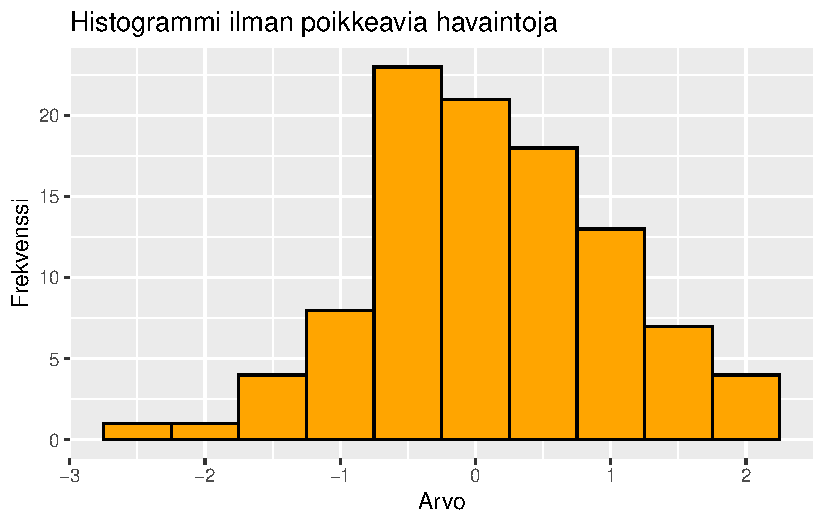
\includegraphics[keepaspectratio]{Tilastotiede/PoikkeavatHavainnot_files/figure-pdf/unnamed-chunk-4-1.pdf}}

\chapter{Normaalisuuden testaaminen}\label{normaalisuuden-testaaminen}

\section{Kolmogorov-smirnov normaalisuustesti
ks.test()}\label{kolmogorov-smirnov-normaalisuustesti-ks.test}

\begin{itemize}
\item
  Toimii paremmin suurella n:llä kuin shapiro-wilk
\item
  R:llä toimii funktiolla \textbf{ks.test()}
\end{itemize}

\section{Shapiro-wilk normaalisuustesti
shapiro.test()}\label{shapiro-wilk-normaalisuustesti-shapiro.test}

\begin{itemize}
\item
  Toimii pienellä n:llä paremmin kuin kolmogorov-smirnov
\item
  R:ssä funktiolla \textbf{shapiro.test()}
\item
  Samat arvot (Ties): Jos datassasi on paljon samoja arvoja (kuten
  Likert-asteikolla 1-5 usein on), R antaa varoituksen: ``cannot compute
  exact p-value with ties''. K-S-testi on tarkoitettu jatkuville
  muuttujille. Jos data on kovin epäjatkuvaa,
  Shapiro-Wilk~(shapiro.test) on usein parempi vaihtoehto normaalisuuden
  testaukseen. Gemini (2026)
\end{itemize}

\section{Normaalijakauma}\label{normaalijakauma}

\pandocbounded{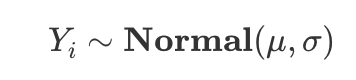
\includegraphics[keepaspectratio]{Tilastotiede/images/clipboard-1108779602.png}}

\begin{quote}
You can read this as ``Yi~is sampled from a Normal distribution with
mean~μ~and standard deviation~σ''. So the tilde (∼) stands for ``sampled
from''.~(Speekenbrink 2023)
\end{quote}

\begin{itemize}
\item
  Kaavassa Yi on siis yksi normaalijakauman havainto
\item
  \textasciitilde{} merkki tarkoittaa, että Y on annetusta jakaumasta
  satunnaisesti otettu alkio
\item
  μ tarkoittaa keskiarvoa
\item
  σ tarkoittaa keskihajontaa
\end{itemize}

\chapter{Matematiikan
laskusääntöjä}\label{matematiikan-laskusuxe4uxe4ntuxf6juxe4}

\section{Kymmenpotenssi (e)}\label{kymmenpotenssi-e}

\begin{itemize}
\item
  R merkkaa kymmenpotensseja tähän tyyliin

  \begin{itemize}
  \item
    p-value \textless{} 2.2e-16
  \item
    e = kymmenpotenssi

    \begin{itemize}
    \item
      2.2e-16 = 2.2 * 10\^{}-16

\begin{Shaded}
\begin{Highlighting}[]
\FunctionTok{format}\NormalTok{(}\FloatTok{2.2} \SpecialCharTok{*} \DecValTok{10}\SpecialCharTok{\^{}{-}}\DecValTok{16}\NormalTok{, }\AttributeTok{scientific =} \ConstantTok{FALSE}\NormalTok{)}
\end{Highlighting}
\end{Shaded}

\begin{verbatim}
[1] "0.00000000000000022"
\end{verbatim}
    \item
      format( ,scientific = FALSE) funktiolla saa esitettyä luvun
      desimaalimuodossa
    \end{itemize}
  \end{itemize}
\item
  Kymmenpotenssissa siirretään aina pilkkua

  \begin{itemize}
  \item
    300 * 10\^{}-2 = 3
  \item
    300 * 10\^{}2 = 30 000
  \end{itemize}
\end{itemize}

\bookmarksetup{startatroot}

\chapter{Summary}\label{summary}

In summary, this book has no content whatsoever.

\begin{Shaded}
\begin{Highlighting}[]
\DecValTok{1} \SpecialCharTok{+} \DecValTok{1}
\end{Highlighting}
\end{Shaded}

\begin{verbatim}
[1] 2
\end{verbatim}

\bookmarksetup{startatroot}

\chapter*{References}\label{references}
\addcontentsline{toc}{chapter}{References}

\markboth{References}{References}

\protect\phantomsection\label{refs}
\begin{CSLReferences}{1}{1}
\bibitem[\citeproctext]{ref-gemini}
Gemini, Google. 2026. \emph{Google Gemini {[}Laaja Kielimalli{]}}.
\url{https://gemini.google.com/}.

\bibitem[\citeproctext]{ref-Rmoniste}
Hyvönen, Ville, Henri Karttunen, Toni Lehtonen, Aku Leivonen, and Savi
Virolainen. 2018. \emph{R-Tutuksi {[}Oppimateriaali{]}}. Helsingin
yliopisto, Matematiikan ja tilastotieteen laitos.
\url{https://www.mv.helsinki.fi/home/mjxpirin/medstat_course/material/Rmoniste_tiltu1.pdf}.

\bibitem[\citeproctext]{ref-navarro2025learning}
Navarro, Danielle, and David Foxcroft. 2025. \emph{Learning Statistics
with JAMOVI: A Tutorial for Beginners in Statistical Analysis}.

\bibitem[\citeproctext]{ref-Salmela}
Salmela, Viljami. 2026. \emph{SPK-3003 {R}-Ohjelmointi 2026
{[}Luentosarja{]}}.

\bibitem[\citeproctext]{ref-analysisandmodelling}
Speekenbrink, M. 2023. \emph{Statistics: Data Analysis and Modelling.}
Open Book Publishers. \url{https://mspeekenbrink.github.io/sdam-book/}.

\bibitem[\citeproctext]{ref-thulin2024modern}
Thulin, Måns. 2024. \emph{Modern Statistics with r: From Wrangling and
Exploring Data to Inference and Predictive Modelling}. Chapman;
Hall/CRC. \url{https://www.modernstatisticswithr.com}.

\bibitem[\citeproctext]{ref-Rdocumentation}
\emph{Www.rdocumentation.org {[}Verkkosivu{]}}. haettu 2026.
\url{https://www.rdocumentation.org}.

\end{CSLReferences}




\end{document}
